
\documentclass[a4paper,10pt,twoside]{ThesisStyle}

\usepackage{amsmath,amssymb}             % AMS Math
\usepackage{lipsum}

%%

\usepackage{ifpdf}
\newcommand\BackgroundPic{
\ifpdf
	\includegraphics[height=\paperheight,width=\paperwidth]{BackgroundTPT_Premiere.eps}
\else
	\includegraphics[height=\paperheight,width=\paperwidth]{BackgroundTPT_Premiere.eps}
\fi
}


%%
\usepackage{latexsym}
\usepackage{graphicx}
\usepackage{ucs}
\usepackage[utf8]{inputenc}
\usepackage{eurosym}
\usepackage[french,english]{babel}
%%
%\usepackage[francais]{babel}
%\usepackage[latin1]{inputenc}
\usepackage[T1]{fontenc}
% \usepackage{times}
\usepackage[left=1.5in,right=1.3in,top=1.1in,bottom=1.1in,includefoot,includehead,headheight=13.6pt]{geometry}
\renewcommand{\baselinestretch}{1.05}

% Table of contents for each chapter

\usepackage[nottoc, notlof, notlot]{tocbibind}
\usepackage{minitoc}
\setcounter{minitocdepth}{3}
\mtcindent=15pt
% Use \minitoc where tos put a table of contents

\usepackage{aecompl}

% Glossary / list of abbreviations

\usepackage[intoc]{nomencl}
\renewcommand{\nomname}{List of Abbreviations}
\makenomenclature

% My pdf code

\usepackage{ifpdf}
\usepackage{graphicx}
%\ifpdf
%  \usepackage[pdftex]{graphicx}
%  %\DeclareGraphicsExtensions{.jpg}
%  %\usepackage[a4paper,pagebackref=false,hyperindex=true]{hyperref}
%\else
%  \usepackage{graphicx}
%  %\DeclareGraphicsExtensions{.ps,.eps}
%  %\usepackage[a4paper,dvipdfm,pagebackref=false,hyperindex=true]{hyperref}
%\fi

\graphicspath{{.}{images/}}

% Links in pdf
\usepackage{color}
\definecolor{linkcol}{rgb}{0,0,0.4} 
\definecolor{citecol}{rgb}{0.5,0,0} 

% Change this to change the informations included in the pdf file

% See hyperref documentation for information on those parameters
\usepackage{hyperref}
\hypersetup
{
bookmarksopen=true,
pdftitle="First class futures",
pdfauthor="Muhammad Uzair KHAN", 
pdfsubject="update strategies for first class futures", %subject of the document
%pdftoolbar=false, % toolbar hidden
pdfmenubar=true, %menubar shown
pdfhighlight=/O, %effect of clicking on a link
colorlinks=true, %couleurs sur les liens hypertextes
pdfpagemode=None, %aucun mode de page
pdfpagelayout=SinglePage, %ouverture en simple page
pdffitwindow=true, %pages ouvertes entierement dans toute la fenetre
linkcolor=linkcol, %couleur des liens hypertextes internes
citecolor=citecol, %couleur des liens pour les citations
urlcolor=linkcol %couleur des liens pour les url
}

% definitions.
% -------------------

\setcounter{secnumdepth}{3}
\setcounter{tocdepth}{2}

% Some useful commands and shortcut for maths:  partial derivative and stuff

\usepackage [table]{xcolor}


\newcommand{\pd}[2]{\frac{\partial #1}{\partial #2}}
\def\abs{\operatorname{abs}}
\def\argmax{\operatornamewithlimits{arg\,max}}
\def\argmin{\operatornamewithlimits{arg\,min}}
\def\diag{\operatorname{Diag}}
\newcommand{\eqRef}[1]{(\ref{#1})}

\usepackage{rotating}                    % Sideways of figures & tables
%\usepackage{bibunits}
%\usepackage[sectionbib]{chapterbib}          % Cross-reference package (Natural BiB)
%\usepackage{natbib}                  % Put References at the end of each chapter
                                         % Do not put 'sectionbib' option here.
                                         % Sectionbib option in 'natbib' will do.
\usepackage{fancyhdr}                    % Fancy Header and Footer

% \usepackage{txfonts}                     % Public Times New Roman text & math font
  
%%% Fancy Header %%%%%%%%%%%%%%%%%%%%%%%%%%%%%%%%%%%%%%%%%%%%%%%%%%%%%%%%%%%%%%%%%%
% Fancy Header Style Options

\pagestyle{fancy}                       % Sets fancy header and footer
\fancyfoot{}                            % Delete current footer settings

%\renewcommand{\chaptermark}[1]{         % Lower Case Chapter marker style
%  \markboth{\chaptername\ \thechapter.\ #1}}{}} %

%\renewcommand{\sectionmark}[1]{         % Lower case Section marker style
%  \markright{\thesection.\ #1}}         %

\fancyhead[LE,RO]{\bfseries\thepage}    % Page number (boldface) in left on even
% pages and right on odd pages
\fancyhead[RE]{\bfseries\nouppercase{\leftmark}}      % Chapter in the right on even pages
\fancyhead[LO]{\bfseries\nouppercase{\rightmark}}     % Section in the left on odd pages

\let\headruleORIG\headrule
\renewcommand{\headrule}{\color{black} \headruleORIG}
\renewcommand{\headrulewidth}{1.0pt}
\usepackage{colortbl}
\arrayrulecolor{black}

\fancypagestyle{plain}{
  \fancyhead{}
  \fancyfoot{}
  \renewcommand{\headrulewidth}{0pt}
}

% \usepackage{algorithm}
% \usepackage{algpseudocode}
% \usepackage{algorithmic}
% \usepackage[ruled,vlined]{algorithm2e}
%%% Clear Header %%%%%%%%%%%%%%%%%%%%%%%%%%%%%%%%%%%%%%%%%%%%%%%%%%%%%%%%%%%%%%%%%%
% Clear Header Style on the Last Empty Odd pages
\makeatletter

\def\cleardoublepage{\clearpage\if@twoside \ifodd\c@page\else%
  \hbox{}%
  \thispagestyle{empty}%              % Empty header styles
  \newpage%
  \if@twocolumn\hbox{}\newpage\fi\fi\fi}

\makeatother
 
%%%%%%%%%%%%%%%%%%%%%%%%%%%%%%%%%%%%%%%%%%%%%%%%%%%%%%%%%%%%%%%%%%%%%%%%%%%%%%% 
% Prints your review date and 'Draft Version' (From Josullvn, CS, CMU)
\newcommand{\reviewtimetoday}[2]{\special{!userdict begin
    /bop-hook{gsave 20 710 translate 45 rotate 0.8 setgray
      /Times-Roman findfont 12 scalefont setfont 0 0   moveto (#1) show
      0 -12 moveto (#2) show grestore}def end}}
% You can turn on or off this option.
% \reviewtimetoday{\today}{Draft Version}
%%%%%%%%%%%%%%%%%%%%%%%%%%%%%%%%%%%%%%%%%%%%%%%%%%%%%%%%%%%%%%%%%%%%%%%%%%%%%%% 

\newenvironment{maxime}[1]
{
\vspace*{0cm}
\hfill
\begin{minipage}{0.5\textwidth}%
%\rule[0.5ex]{\textwidth}{0.1mm}\\%
\hrulefill $\:$ {\bf #1}\\
%\vspace*{-0.25cm}
\it 
}%
{%

\hrulefill
\vspace*{0.5cm}%
\end{minipage}
}

\let\minitocORIG\minitoc
\renewcommand{\minitoc}{\minitocORIG \vspace{1.5em}}

\usepackage{multirow}
\usepackage{slashbox}

\newenvironment{bulletList}%
{ \begin{list}%
	{$\bullet$}%
	{\setlength{\labelwidth}{25pt}%
	 \setlength{\leftmargin}{30pt}%
	 \setlength{\itemsep}{\parsep}}}%
{ \end{list} }

\newtheorem{definition}{D?finition}
\renewcommand{\epsilon}{\varepsilon}

% centered page environment

\newenvironment{vcenterpage}
{\newpage\vspace*{\fill}\thispagestyle{empty}\renewcommand{\headrulewidth}{0pt}}
{\vspace*{\fill}}
\usepackage{verbatim}
%\usepackage{minitoc}
%\usepackage{wrapfig}
\usepackage{listings}
\usepackage{hyperref}
\hypersetup{
    bookmarks=true,         % show bookmarks bar?
    unicode=false,          % non-Latin characters in Acrobat?s bookmarks
    pdftoolbar=true,        % show Acrobat?s toolbar?
    pdfmenubar=true,        % show Acrobat?s menu?
    pdffitwindow=false,     % window fit to page when opened
    pdfstartview={FitH},    % fits the width of the page to the window
    pdftitle={My title},    % title
    pdfauthor={Author},     % author
    pdfsubject={Subject},   % subject of the document
    pdfcreator={Creator},   % creator of the document
    pdfproducer={Producer}, % producer of the document
    pdfkeywords={keyword1} {key2} {key3}, % list of keywords
    pdfnewwindow=true,      % links in new window
    colorlinks=false,       % false: boxed links; true: colored links
    linkcolor=red,          % color of internal links
    citecolor=green,        % color of links to bibliography
    filecolor=magenta,      % color of file links
    urlcolor=cyan           % color of external links
}

\newcommand{\todo}[1]{\textcolor{red}{%
\raisebox{-0.2em}[0pt][0pt]{\makebox[0pt]{\rule{1pt}{1.1em}}\makebox[0pt][l]{\raisebox{1em}{\rule{5ex}{1pt}}}}
\textbf{TODO:} \textit{#1}
\raisebox{-0.2em}[0pt][0pt]{\makebox[0pt][r]{\rule{5ex}{1pt}}\makebox[0pt]{\rule{1pt}{1em}}}%
}}

\newcommand{\comments}[1]{\textcolor{blue}{%
\raisebox{-0.2em}[0pt][0pt]{\makebox[0pt]{\rule{1pt}{1.1em}}\makebox[0pt][l]{\raisebox{1em}{\rule{5ex}{1pt}}}}
\textbf{COMMENTS:} \textit{#1}
\raisebox{-0.2em}[0pt][0pt]{\makebox[0pt][r]{\rule{5ex}{1pt}}\makebox[0pt]{\rule{1pt}{1em}}}%
}}

%\usepackage[dvips]{graphicx, color}
%\usepackage[bookmarks=true, bookmarksnumbered=true,hypertexnames=false, breaklinks=true]{hyperref}
%\DeclareGraphicsExtensions{.eps,.ps}

\newlength{\plarg}
\setlength{\plarg}{16cm}
\newlength{\glarg}
\setlength{\glarg}{17cm}
\lstset{
         basicstyle=\scriptsize\ttfamily, % Standardschrift
         numbers=left,               % Ort der Zeilennummern
         numberstyle=\tiny,          % Stil der Zeilennummern
         frame=single,
         %stepnumber=2,               % Abstand zwischen den Zeilennummern
         numbersep=5pt,              % Abstand der Nummern zum Text
         tabsize=2,                  % Groesse von Tabs
         extendedchars=true,         %
         breaklines=true,            % Zeilen werden Umgebrochen
         keywordstyle=\color{red},
                frame=b,         
  %       keywordstyle=[1]\textbf,    ]{\index{keywords, BEGIN}}% Stil der Keywords
  %       keywordstyle=[2]\textbf,    %
  %      keywordstyle=[3]\textbf,    %
 %        keywordstyle=[4]\textbf,   \sqrt{\sqrt{}} %
         stringstyle=\color{blue}\ttfamily, % Farbe der String
         showspaces=false,           % Leerzeichen anzeigen ?
         showtabs=false,             % Tabs anzeigen ?
         xleftmargin=17pt,
         framexleftmargin=17pt,
         framexrightmargin=5pt,
         framexbottommargin=4pt,
       	% backgroundcolor=\color{gray},
         showstringspaces=false,   
         language= C++, 
         captionpos=b, 
         caption=Platform Integrity Aspect, % Leerzeichen in Strings anzeigen ?        
 }


\listfiles
  
\setlength{\parindent}{0pt}

\newcommand\CyrGuillemot{%
  \def\selectguillfont{\fontencoding{OT2}\fontfamily{wncyr}\selectfont}
  \def\guillemotleft{\selectguillfont\symbol{60}}
  \def\guillemotright{\selectguillfont\symbol{62}}
}

\newcommand\PlGuillemot{%
  \def\selectguillfont{\fontencoding{OT4}\fontfamily{cmr}\selectfont}
  \def\guillemotleft{\selectguillfont\symbol{174}}
  \def\guillemotright{\selectguillfont\symbol{175}}
}

\newcommand\LaGuillemot{%
  \def\selectguillfont{\fontencoding{U}\fontfamily{lasy}%
    \fontseries{m}\fontshape{n}\selectfont}
  \def\guillemotleft{\selectguillfont\hbox{\symbol{40}%
    \kern-0.20em\symbol{40}}}
  \def\guillemotright{\selectguillfont\hbox{\symbol{41}%
    \kern-0.20em\symbol{41}}}
}

\newcommand\ECGuillemot{%
  \def\selectguillfont{\fontencoding{T1}\fontfamily{cmr}\selectfont}
  \def\guillemotleft{\selectguillfont\symbol{19}}
  \def\guillemotright{\selectguillfont\symbol{20}}
}

\newcommand\LMGuillemot{%
  \def\selectguillfont{\fontencoding{T1}\fontfamily{lmr}\selectfont}
  \def\guillemotleft{\selectguillfont\symbol{19}}
  \def\guillemotright{\selectguillfont\symbol{20}}
}

\newcommand\CyrGLeft{\CyrGuillemot\guillemotleft}
\newcommand\CyrGRight{\CyrGuillemot\guillemotright}
\newcommand\PlGLeft{\PlGuillemot\guillemotleft}
\newcommand\PlGRight{\PlGuillemot\guillemotright}
\newcommand\LaGLeft{\LaGuillemot\guillemotleft}
\newcommand\LaGRight{\LaGuillemot\guillemotright}
\newcommand\ECGLeft{\ECGuillemot\guillemotleft}
\newcommand\ECGRight{\ECGuillemot\guillemotright}
\newcommand\LMGLeft{\LMGuillemot\guillemotleft}
\newcommand\LMGRight{\LMGuillemot\guillemotright}



\newcommand{\algorithmicrequire}{\textbf{Require:}}
\newcommand{\algorithmicensure}{\textbf{Ensure:}}


% \usepackage{graphicx}
\usepackage{url}
\usepackage{listings}
\usepackage{psfrag}
\usepackage{array,xspace}
\usepackage{epsfig,color,subfig,graphics}
%\usepackage{epsfig,graphics,subfigure,graphicx,latexsym,longtable,amsmath,amscd,amsthm,latexsym,amssymb,mathrsfs,syntonly,eucal}

\usepackage[belowskip=-12pt,aboveskip=7pt]{caption}

\usepackage {mathpartir,amssymb,stmaryrd,mathtools}
\usepackage{alltt}
\usepackage{amsmath}
\usepackage{multirow}
\usepackage{color}

\usepackage{booktabs}
% \usepackage{epstopdf}
%\usepackage{todonotes}
\usepackage{longtable}
\usepackage{pdflscape}
\usepackage{algorithm}
\usepackage{algorithmic}
% \usepackage[ruled,vlined]{algorithm2e}
\usepackage{cases}
% \usepackage[retainorgcmds]{IEEEtrantools}
\usepackage{wrapfig}
%\usepackage[table]{xcolor}
%\usepackage{subfigure}
% \documentclass{llncs}
% \usepackage{graphicx,url}
% \usepackage{llncsdoc}
%\usepackage{listings}
%\usepackage{array,xspace}
%\usepackage{epsfig,color,subfigure}
%\usepackage {mathpartir,amssymb,stmaryrd,mathtools}
%
%\usepackage{apacite}
%\usepackage{bibunits}
% my list of commands and defs%
\def\ttbraces{\let\.=\nobreak\chardef\{=`\{\chardef\}=`\}\chardef\|=`\\}

\newcommand{\TODO}[1]{\textcolor{red}{\textbf{[TODO:#1]}}}

\newenvironment{ttbox}{
 \begin{center}\vspace{-.5ex}
     \begin{tabular}{@{}|@{\,}c@{\,}|@{}}
\hline\\[-2ex]
\begin{minipage}[b]{.98\linewidth}
\begin{alltt}\ttbraces\small} 
                     {\end{alltt}
     \end {minipage}\\[.3ex]
  \hline
\end{tabular}
\end{center}}

\newcommand{\symb}[1]{\makebox{\it #1}}
% shorthand for various frameworks

%\def \abclf {ABCL/f\;}
\def \proactive {ProActive} 
\newcommand{\aspfun}{ASP${}_\text{fun}$\xspace}
\newcommand{\ttt}[1] {\texttt{#1}} 


\newenvironment{myitemize}
{\begin{itemize}%\addtolength{\itemsep}{-0.5\baselineskip}
\addtolength{\leftskip}{-1.5ex}
\vspace{-.1ex}} 
{\end{itemize}\addtolength{\leftskip}{1.5ex}}
%%%%%%%%%%%%%%%%%%%%%%%%%%%%%%%%%%%%%%%%%%%%%%%%%%%%%%%
\newcommand\rbeta{\to_{\beta}}
\newcommand\rbetastar{{\to_{\beta}^*}}
\newcommand\parbeta{\Rightarrow_{\beta}}
\newcommand\gle{\sqsubseteq}
\newcommand\ttgle{\mbox{\( \gle \)}}
\newcommand\eps{\varepsilon}
\newcommand\eg{e.g.\ }
\newcommand\ie{i.e.\ }
\newcommand\cf{c.f.\ }
\newcommand\etal{{\it et al.} \ }
\newcommand\ttcl{pre\_cl}
\newcommand\ttsp{\mbox{\( sp \)}}
\newcommand\ttwp{\mbox{\( wp \)}}
\newcommand\ttRinv{R\mbox{\( ^{-1} \)}}
\newcommand\oim{\mbox{\(\llparenthesis\)}}
\newcommand\cim{\mbox{\(\rrparenthesis\)}}
\newcommand\imp\Rightarrow
\newcommand\ttrapp{"}
%generally used
\newcommand\tthash{\mbox{\tt \#}}
\newcommand\ttcirc{\mbox{\( \circ\)}}
\newcommand\ttforall{\mbox{\( \forall \)}}
\newcommand\ttexists{\mbox{\( \exists \)}}
\newcommand\ttequiv{\mbox{\( \equiv \)}}
\newcommand\ttexistsun{\mbox{\( \exists^1 \)}}
\newcommand\ttin{\mbox{\(\in\)}}
\newcommand\ttnin{\mbox{\(\notin\)}}
\newcommand\ttTimes{\mbox{\(\times\)}}
\newcommand\ttalpha{\mbox{\( \alpha \)}}
\newcommand\ttbeta{\mbox{\( \beta \)}}
\newcommand\ttlam{\mbox{\( \lambda \)}}
\newcommand\ttsig{\mbox{\( \sigma \)}}
\newcommand\tteps{\mbox{\( \varepsilon \)}}
\newcommand\ttOmega{\mbox{\( \Omega \)}}
\newcommand\ttpi{\mbox{\( \pi \)}}
\newcommand\ttgam{\mbox{\( \gamma \)}}
\newcommand\ttneg{\mbox{\( \lnot \)}}
\newcommand\ttor{\mbox{\( \lor \)}}
\newcommand\ttwedge{\mbox{\( \land \)}}
\newcommand\ttimp{\mbox{\( \longrightarrow\)}}
\newcommand\ttImp{\mbox{\( \Longrightarrow\)}}
\newcommand\ttfun{\mbox{\( \Rightarrow\)}}
\newcommand\ttssubseteq{\mbox{\( \subseteq\)}}
\newcommand\ttrbeta{\mbox{\( \rbeta\)}}
\newcommand\ttred{\mbox{\( \to_R\)}}
\newcommand\ttuparrow{\mbox{\( \uparrow\)}}
\newcommand\ttfred{\mbox{\( \to_F\)}}
\newcommand\ttored{\mbox{\( \to_O\)}}

\newcommand\ttrbetastar{\mbox{\( \rbetastar\)}}
\newcommand\ttparbeta{\mbox{\( \parbeta\)}}
\newcommand\ttneq{\mbox{\( \neq \)}}
\newcommand\ttbigcup{\mbox{\( \bigcup \)}}
\newcommand\ttcap{\mbox{\( \cap \)}}
\newcommand\ttcup{\mbox{\( \cup \)}}
\newcommand\ttdef{\mbox{\( \equiv_{df} \)}}
\newcommand\ttsubset{\mbox{\( \subseteq \)}}
\newcommand\tttimes{\mbox{\( \times \)}}
\newcommand\ttvdash{\mbox{\( \vDash \)}}
\newcommand\ttvdashs{\mbox{\( \vdash \)}}
\newcommand\ttleq{\mbox{\( \leq \)}}
\newcommand\ttmapsto{\mbox{\( \mapsto \)}}
\newcommand\ttleftarrow{\mbox{\( \gets \)}}
\newcommand\ttleadsto{\mbox{\( \leadsto \)}}
\newcommand\ttrefone{\mbox{\( (1)\)}}
\newcommand\ttreftwo{\mbox{\( (2)\)}}
\newcommand\ttlbrack{\mbox{\(\llbracket\)}}
\newcommand\ttrbrack{\mbox{\( \rrbracket \)}}
\newcommand\ttstar{\mbox{\({}^*\)}}
\newcommand\ttmetaall{\mbox{\( \bigwedge \)}}
\newcommand\ttminusone{\mbox{\({}^{-1}\)}}
\newcommand{\oarrow}[3]{\,\relbar\Mapsfromchar\!#1,#2,#3\!\Mapstochar\to} 


\newcommand\ttoarrow[3]{\mbox{\(\relbar\Mapsfromchar\)}#1,#2,#3\mbox{\(\Mapstochar\to_O\)}}

\newcommand\ttfarrow[3]{\mbox{\(\relbar\Mapsfromchar\)}#1,#2,#3\mbox{\(\Mapstochar\to_F\)}}
\newcommand\ttsubi{\mbox{\({}_{i}\)}}
\newcommand \keyword[1]{\textcolor{red}{\bf{#1}}}


%\def\ttbraces{\let\.=\nobreak\chardef\{=`\{\chardef\}=`\}\chardef\|=`\\}

\DeclareMathOperator{\futs}{futs}
\DeclareMathOperator{\Prim}{Prim}
\DeclareMathOperator{\Comp}{Comp}
\DeclareMathOperator{\Enqueue}{Enqueue}
\DeclareMathOperator{\findResult}{findRes}
\DeclareMathOperator{\dom}{dom}




%%%%%%%%%%%%%%%%%%%%%%%%%%%%%%%%%%%%%%%%%%%%%%%%%%%%%%%%%




%%% Local Variables: 
%%% mode: latex
%%% TeX-master: "Thesis"
%%% End: 


\usepackage{pdfpages}
\usepackage{imakeidx}


\makeatletter
\renewcommand{\@chapapp}{}% Not necessary...
\newenvironment{chapquote}[2][2em]
  {\setlength{\@tempdima}{#1}%
   \def\chapquote@author{#2}%
   \parshape 1 \@tempdima \dimexpr\textwidth-2\@tempdima\relax%
   \itshape}
  {\par\normalfont\hfill--\ \chapquote@author\hspace*{\@tempdima}\par\bigskip}
\makeatother
\makeindex
%\usepackage[left=1.3cm,top=0cm,right=1.3cm,bottom=1.2cm]{geometry}
%\usepackage{graphicx}
%\usepackage{eso-pic}
%\usepackage{array}
%\usepackage[french]{babel}
%\usepackage[utf8x]{inputenc}
%\usepackage[T1]{fontenc}
%\usepackage{textcomp}
%\usepackage{helvet}	% or \usepackage{lmodern}
%\renewcommand\textnumero{n$^{\textsf{{\tiny O}}}$}
%\renewcommand{\familydefault}{\sfdefault}

\begin{document}
{

\begin{titlepage}
%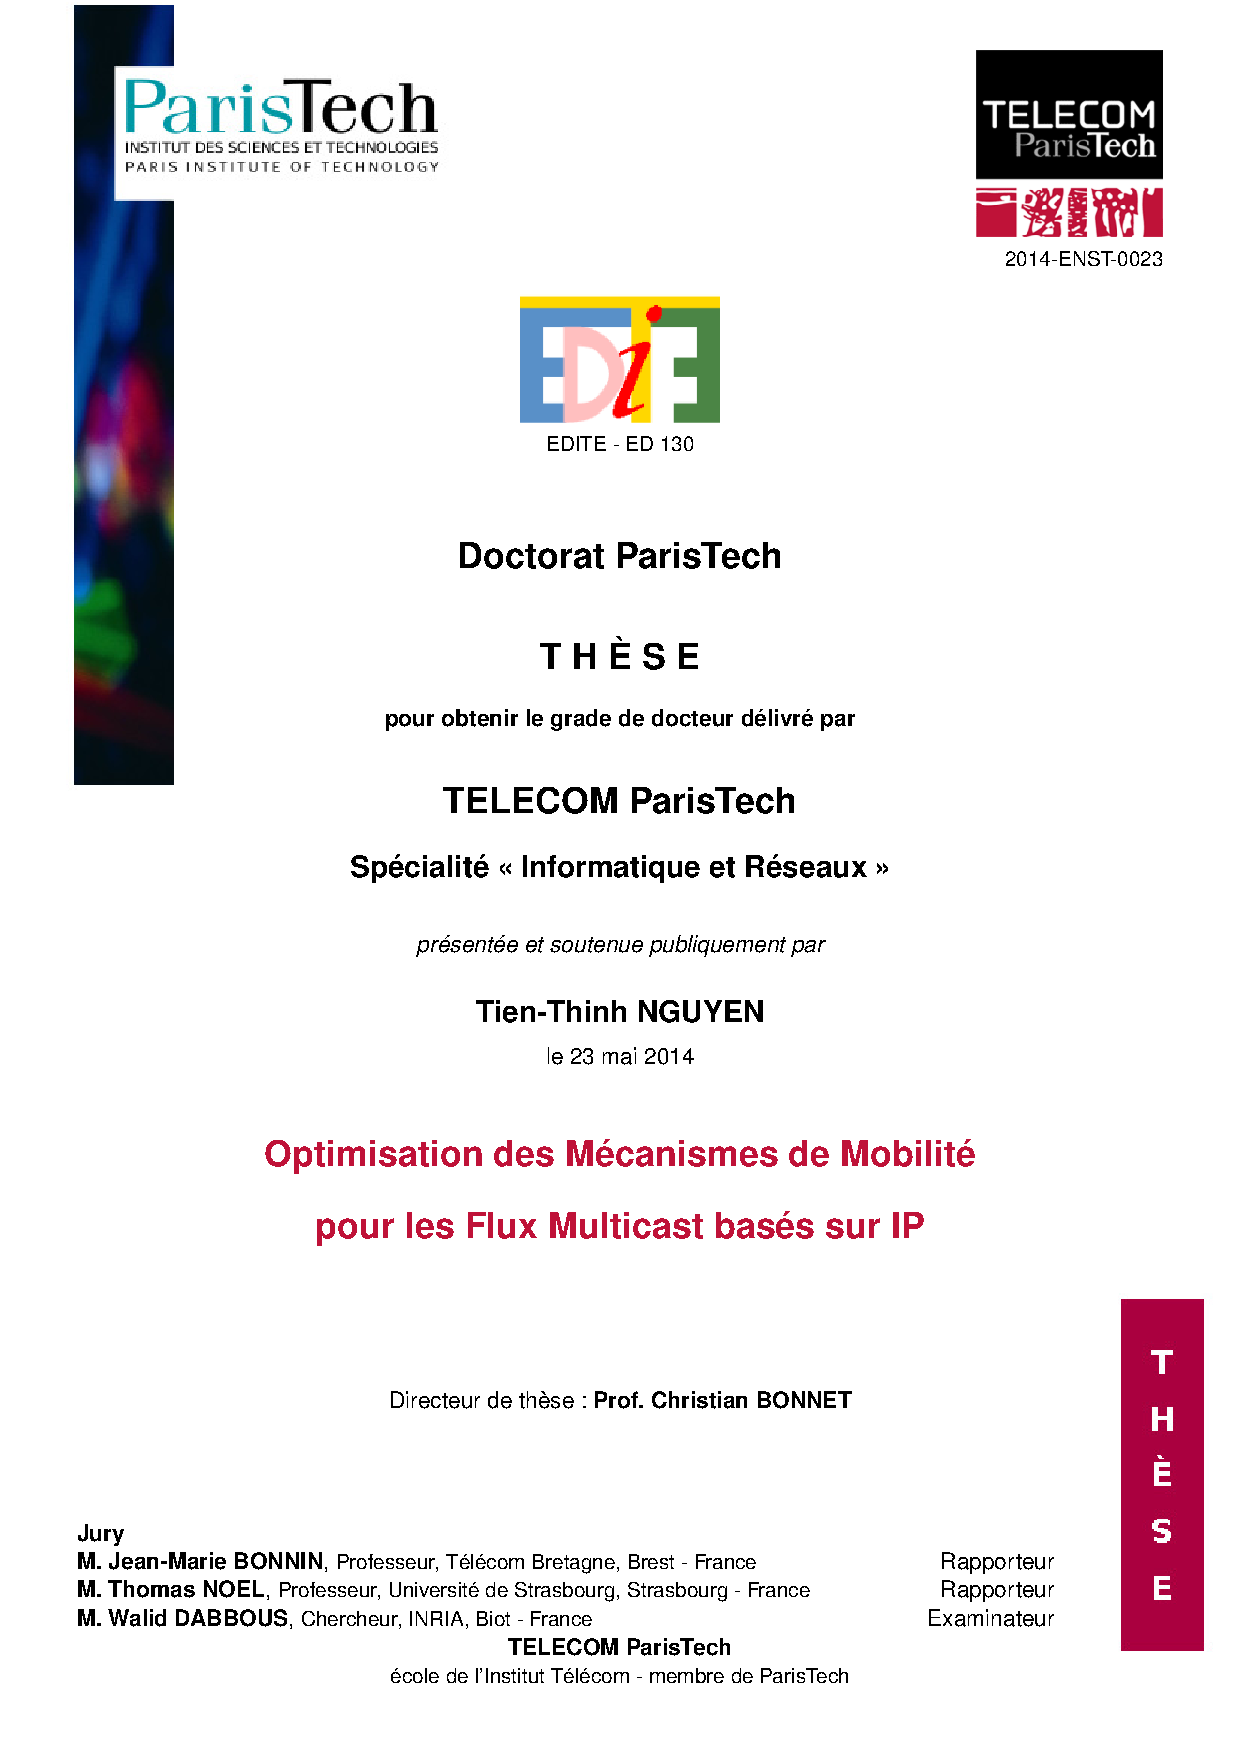
\includepdf[pages={1}]{TPT_Premiere.pdf}

  \vspace{10mm}
  \noindent




	\begin{center}
	
\includegraphics[width=48mm]{logo_ParisTech}
	\end{center}

  \vspace{5mm}


\center

\begin{bfseries}
  \noindent{\LARGE INTEROPERATION MECHANISM FOR INDUSTRIAL INTERNET OF THINGS 
\vspace{4mm}
  \\ APPLICATION AND SMART CITY.}
  \vspace{15mm}

  \noindent{\Large Kim-Hung Le}
  \vspace{10mm}
\end{bfseries}


\noindent{A doctoral dissertation submitted to:}

\vspace{2mm}

\noindent{TELECOM ParisTech}

\vspace{2mm}

\noindent{In Partial Fulfillment of the Requirements for the Degree of:}

\vspace{2mm}

\noindent{\textbf{Doctor of Philosophy}}

\vspace{2mm}

\noindent{Specialty : \textsc{Computer Science and Networking}}

\vspace{2mm}




% \vspace{6mm}

% \noindent{ \large \textit{Thesis Supervisor:} ~~\textbf{Prof.\ Christian \textsc{Bonnet}}\\	\hspace{2mm}\textbf{Prof.\ Paolo \textsc{Papotti}}}

% \vspace{2mm}
 
 
% \begin{center}
% \noindent \large 
% \begin{tabular}{llcl}
%       \textit{Jury:}	& 		& & \\\\
%      \textit{Reviewers:} & & & \\
%  \multicolumn{2}{l}{~~\textbf{Prof.\ Thomas \textsc{Noel} }} 		& - & Universit\'{e} de Strasbourg, Strasbourg - France\\
%  \multicolumn{2}{l}{~~\textbf{Prof.\ Jean-Marie \textsc{Bonnin}}} 		& - &  T\'{e}l\'{e}com Bretagne, Brest - France\\
% \\
%       \textit{Examiner:}& 		& & \\
      
% \multicolumn{2}{l}{~~\textbf{Dr. \ Walid \textsc{Dabbous}}}           & - & INRIA, Biot - France\\
% \\


  
% \end{tabular}
% \end{center}

\end{titlepage}

}


\cleardoublepage

\pagenumbering{gobble}
\vspace{10mm}

\hfill
  \noindent{
\vspace{4mm}}


\begin{center}
\noindent \large 
\vspace{32mm}
\noindent{\textbf{To my wife and my little son - Bi}}
 \end{center}

\vspace{3cm}
\dominitoc
\pagenumbering{roman}
\cleardoublepage


%\section*{}
% \vspace{118ex}
% \begin{center}
% \copyright \hspace{1ex}2012\\Tien-Thinh NGUYEN\\ALL RIGHTS RESERVED
% \end{center}
% \cleardoublepage


\addcontentsline{toc}{section}{Acknowledgements}
\markboth{Acknowledgements}{Acknowledgements}
\chapter*{Acknowledgements}

% First of all, I would like to extend my sincere thanks to my advisor Prof. Christian Bonnet for his valuable support and brilliant ideas. Throughout this thesis, he has always found the time for me to guide and encourage my research activities. I also very much appreciate his dynamism and his competences that made this thesis work a success. It has been my real pleasure to work with Christian. \\

% I would also like to thank Prof. Jérôme Härri who helped me so much with his stimulating technical discussions and constructive publication reviewing. A special warm thank to my master advisor Michelle Wetterwald for her kindness and words of wisdom which facilitate not only my research but also my life.\\

% I am grateful to the committee members of my jury, Prof. Jean-Marie Bonnin, Prof. Thomas Noël and M. Walid Dabbous for their valuable inputs and time spent reading this thesis. \\

% I would like to express my appreciation to my colleagues and friends at Eurecom, for all the unforgettable enjoyable moments and their helps. I also wish to extend my warmest thanks to all my friends in France and Vietnam for all the wonderful time we spend together.\\

% Finally, last but not least, I want to express my special gratitude to my parents, my wife and my son for their unconditional support, love and trust. They, together with another members in my big family, make my life full of kindness and happiness with their encouragement.\\

\addcontentsline{toc}{section}{Abstract}
\markboth{Abstract}{Abstract}
\chapter*{Abstract}
% With the development of wireless access technology as well as the explosion of mobile devices (such as smartphones, tablets, and vehicles), the next generation mobile network is not only restricted to provide the traditional voice services but also the data services. Also, the increasing penetration of the mobile devices is generating a huge number of data traffic over mobile networks. In all-IP mobile networks, IP mobility management is a crucial concept to meet the demand of ubiquitous Internet connectivity as well as new service requirements such as seamless handover across heterogeneous networks, consistent quality of experience and stringent delay constraints. In this context, the scalability and bandwidth efficiency from the multicast routing make the IP multicast a valuable solution from the application point of view to deal with a huge number of traffic, particularly, in mobile environments where users usually share frequency bands and limited capacity. But one of the major challenges for the multicast support is when considering mobility. It comes from the fact that the multicast protocols were designed to support the stationary multicast parties. As such, it raises some issues as a result of the interaction of IP multicast and IP mobility protocols such as service interruption, packet loss, routing non-optimal, and packet duplication, etc. In fact, the conventional IP mobility management (e.g., Mobile IPv6 (MIPv6) and Proxy Mobile IPv6 (PMIPv6)) which leverages on the centralized mobility management approach, brings several issues for the network operator like inefficient use of network resources, poor performance, and scalability issues. The concept of Distributed Mobility Management (DMM) aims to tackle these issues and helps the mobile operators address the challenges created by rising mobile usage while enhancing the overall customer experience.\\

% In this thesis, our main objective is to deal with the multicast mobility-related issues. The solutions are proposed in the context of the evolution of the current IP mobility management: from the host-based to the network-based, and also from the centralized to the distributed mobility management. In more details, for a single PMIPv6 domain, we introduce a method to reduce the service disruption and leave latency. We then present a solution from the load balancing point of view to address the service disruption and packet duplication issue. As DMM has not been standardized, we propose an inter-domain mobility solution, which can be considered as a step in the evolution from PMIP towards DMM. Finally, we converge to a final architecture in a DMM environment that can offer various benefits and address most of the multicast listener mobility-related issues. Throughout this thesis, a near-to-real testbed is used to achieve the realistic results.

aa \index{aa}

\clearpage


\addcontentsline{toc}{section}{Contents}
\markboth{Contents}{Contents}

\tableofcontents
\clearpage

\addcontentsline{toc}{section}{List of Figures}
\listoffigures
\clearpage
\addcontentsline{toc}{section}{List of Tables}
\listoftables
\clearpage

%\printnomenclature
\addcontentsline{toc}{section}{Glossary}
\markboth{Glossary}{Glossary}
\chapter*{Glossary}
List of Abbreviations and Acronyms\\
\\
% \begin{center}
% \begin{longtable}{p{5cm}p{8.8cm}}
% % % \hline
% \textbf{3GPP} & 3rd Generation Partnership Project\\
% \textbf{4G} & Fourth Generation\\
% \textbf{AAA} & Authentication, Authorization and Accounting\\
% \textbf{ALM} & Application-Layer Multicast\\
% \textbf{ASM} & Any-Source Multicast\\
% \textbf{aHMAR} & Anchor HMAR \\
% \textbf{aNMAR} & Anchor NMAR\\
% \textbf{AP} & Access Point\\
% \textbf{AR} & Access Router\\
% \textbf{A-LMA} & Anchor LMA\\
% \textbf{A-AAA} & Anchor AAA\\
% \textbf{A-MAG} & Anchor MAG\\
% \textbf{BA} & Binding Acknowledgment\\
% \textbf{BCE} & Binding Cache Entry\\
% \textbf{BU} & Binding Update\\
% \textbf{CBT} & Core Based Tree \\
% \textbf{CDN} & Content Delivery Network\\
% \textbf{cHMAR} & Current HMAR \\
% \textbf{C-LBC} & Central Load Balancing Controller\\
% \textbf{cMAR} & Current MAR\\
% \textbf{CMD} & Centralized Mobility Database\\
% \textbf{CMF} & Context Management Function\\
% \textbf{cNMAR} & Current NMAR\\
% \textbf{CN} & Corresponding Node\\
% \textbf{CoA} & Care-of-Address\\
% \textbf{COMMA} & Common MMA\\
% \textbf{DHCP} & Dynamic Host Configuration Protocol\\
% \textbf{DMM} & Distributed Mobility Management\\
% \textbf{DMMA} & Dynamic Multicast Mobility Anchor\\
% \textbf{DSMIPv6} & Dual Stack Mobile IPv6\\
% \textbf{DR} & Designated Router\\
% \textbf{DVMRP} & Distance Vector Multicast Routing Protocol \\
% \textbf{D-GW} & Distributed Gateway\\
% \textbf{eNB} & Evolved NodeB\\
% \textbf{EPC} & Evolved Packet Core\\
% \textbf{ETF} & Explicit Tracking Function\\
% \textbf{EV} & Electric Vehicle\\
% \textbf{EVCS} & Electric Vehicle Charging Service\\
% \textbf{FA} & Foreign Agent\\
% \textbf{FI} & Fairness Index\\
% \textbf{FMIPv6} & Fast Mobile IPv6\\
% \textbf{FPMIPv6} & Fast Handovers for PMIPv6\\
% \textbf{GGSN} & Gateway GPRS Support Node\\
% \textbf{GPRS} & General packet radio service\\
% \textbf{G2V} & Grid-to-Vehicle\\
% \textbf{HA} & Home Agent\\
% \textbf{HMAR} & Host-based Mobile Access Router \\
% \textbf{HMIPv6} & Hierarchical Mobile IPv6\\
% \textbf{HeNB} & Home eNodeB\\
% \textbf{HIP} & Host Identity Protocol \\
% \textbf{HNP} & Home Network Prefix\\
% \textbf{HoA} & Home Address\\
% \textbf{HSPA} & High Speed Packet Access\\

% \textbf{IANA} & Internet Assigned Number Authority \\
% \textbf{ICMD} & Inter-Domain Centralized Mobility Database\\
% \textbf{IETF} & Internet Engineering Task Force\\
% \textbf{IGMP} & Internet Group Management Protocol\\
% \textbf{IFOM} & IP Flow Mobility\\
% \textbf{IMR} & Intersection Multicast Router\\
% \textbf{IP} & Internet Protocol\\
% \textbf{IPTV} & Internet Protocol Television\\

% \textbf{L2} & Layer 2\\
% \textbf{L3} & Layer 3\\
% \textbf{LB} & Load Balancing\\
% \textbf{LBC} & Load Balancing Controller\\
% \textbf{LIPA} & Local IP Access \\
% \textbf{LLQC} & Last Listener Query Count \\
% \textbf{LLQT} & Last Listener Query Timer \\
% \textbf{LMA} & Local Mobility Anchor\\
% \textbf{LMD} & Localized Mobility Domain\\
% \textbf{LTE} & Long Term Evolution\\
% \textbf{L-GW} & Local Gateway\\
% \textbf{MAC} & Media Access Control\\
% \textbf{MAG} & Mobile Access Gateway\\
% \textbf{MALI} & Multicast Address Listening Interval\\
% \textbf{MANET} & Mobile Ad hoc Network \\
% \textbf{MAP} & Mobility Anchor Point \\
% \textbf{MAR} & Mobile Access Router \\
% \textbf{MBMS} & Multicast/Broadcast Multimedia Service\\
% \textbf{MBone} & Multicast Backbone\\
% \textbf{MBSFN} & Multicast/Broadcast over a Single Frequency Network\\
% \textbf{MCTF} & Multicast Context Transfer Function\\
% \textbf{MC-Req} & Mobility Context Request \\
% \textbf{MC-Res} & Mobility Context Response \\
% \textbf{MFC} & Multicast Forwarding Cache \\
% \textbf{MGMF} & Multicast Group Management Function \\
% \textbf{MIH} & Media Independent Handover \\
% \textbf{MIPv6} & Mobile IPv6\\
% \textbf{MLD} & Multicast Listener Discovery\\
% \textbf{MMA} & Multicast Mobility Anchor\\
% \textbf{MMAP} & Multicast by Multicast Agent Protocol\\
% \textbf{MMF} & Mobility Management Function \\
% \textbf{MN} & Mobile Node\\
% \textbf{MN-ID} & Mobile Node's Identifier\\
% \textbf{MNP} & Mobile Network Prefix \\
% \textbf{MoM} & Mobile Multicast Protocol \\
% \textbf{MOR} & Mobile Router \\
% \textbf{MOSPF} & Multicast Open Shortest Path First \\
% \textbf{MPDSR} & Multicast Protocol With Dynamic Service Range  \\
% \textbf{MR} & Multicast Router \\
% \textbf{MRIB} & Multicast Routing Information Base \\
% \textbf{MSDP} & Multicast Source Discovery Protocol \\
% \textbf{MTMA} & Multicast Tree Mobility Anchor \\
% \textbf{MUMO} & Multicast Mobility Management Module \\
% \textbf{NAI} & Network Access Identifier\\
% \textbf{ND} & Neighbor Discovery\\
% \textbf{NetLMM} & Network-based Localized Mobility Management  \\
% \textbf{NEMO} & Network Mobility\\
% \textbf{NI} & Node Information\\
% \textbf{NMAR} & Network-based DMM Access Router \\
% \textbf{NS-3} & Network Simulator NS-3 \\

% \textbf{PBA} & Proxy Binding Acknowledgment \\
% \textbf{PBS} & Personal Broadcast Service \\
% \textbf{PBU} & Proxy Binding Update\\
% \textbf{P-GW} & Packet Data Network (PDN) Gateway\\
% \textbf{PIM} & Protocol Independent Multicast\\
% \textbf{PIM-DM} & Protocol Independent Multicast - Dense Mode\\
% \textbf{PIM-SM} & Protocol Independent Multicast - Spare Mode\\
% \textbf{PIM-SSM} & Protocol Independent Multicast - Source Specific Multicast\\
% \textbf{pHMAR} & Previous HMAR \\
% \textbf{PLC} & Power Line Communication \\
% \textbf{pMAR} & Previous MAR\\
% \textbf{PMIPv6} & Proxy Mobile IPv6\\
% \textbf{pNMAR} & Previous NMAR\\
% \textbf{Proxy-CoA} & Proxy Care-of-Address\\

% \textbf{QI} & Query Interval\\
% \textbf{QRI} & Query Response Interval\\

% \textbf{RIB} & Routing Information Base\\
% \textbf{RPF} & Reverse Path Forwarding\\
% \textbf{RV} & Robustness Variable\\

% \textbf{SDN} & Software Defined Networking\\
% \textbf{SGSN} & Serving GPRS Support Node\\
% \textbf{SIP} & Session Initiation Protocol\\
% \textbf{SIPTO} & Selected IP Traffic Offload\\
% \textbf{SMR} & Session-to-mobility Ratio \\
% \textbf{SPT} & Shortest Path Tree \\
% \textbf{SSM} & Source-Specific Multicast\\
% \textbf{S-GW} & Serving Gateway\\
% \textbf{S-AAA} & Serving AAA\\
% \textbf{S-LMA} & Serving LMA\\
% \textbf{S-MAG} & Serving MAG\\

% \textbf{tLMA} & Target LMA\\
% \textbf{TLV} & Type-length- vector\\
% \textbf{tMAR} & Typical location MAR\\

% \textbf{RA} & Router Advertisement \\
% \textbf{RADIUS} & Remote Authentication Dial In User Service\\
% \textbf{RAN} & Radio Access Network \\
% \textbf{RBMoM} & Range-Based Mobile Multicast  \\
% \textbf{RP} & Rendezvous-Point\\
% \textbf{RPT} & Rendezvous-Point Tree\\
% \textbf{RO} & Route Optimization\\
% \textbf{RS} & Router Solicitation\\
% \textbf{RTT} & Round-Trip Time\\

% \textbf{UDP} & User Datagram Protocol \\
% \textbf{UE} & User Equipment \\
% \textbf{UGC} & User Generated Content \\
% \textbf{UML} & User-Mode Linux\\
% \textbf{UNP} & Update Notification Message\\
% \textbf{V2G} & Vehicle-to-Grid\\
% \textbf{VoIP} & Voice over IP\\
% \textbf{WiMAX} & Worldwide Interoperability for Microwave Access\\

% \end{longtable}
% \end{center}

\clearpage

\mainmatter
\chapter{Introduction}
\label{intro}
\section{Motivation and Problem Statement}

Internet of Things (IoT), also known as Internet of Everything (IoE), is a novel paradigm that rapidly gains vast attention in the internet era. The basic idea of IoT is the inter-networking of variety of things through unique addressing scheme, based on standard communication protocol, while ``Things'' is ``an object not precisely identifiable'' - such sensors, actuators, connected tags, mobile phones, etc~\cite{atzori2010internet}\cite{bassi2008internet}. 
The internet of things aims to create a smart environment by bringing the Things in physical world into digital world. In other work, IoT is not only connecting to the Things using the Internet but also enabling data exchange.
Ideally, everything could be connected anytime from anywhere by anyone. Based on such context, 
the massive number of innovative applications will emerge to exploit the benefit of connectivity and accessibility of everything~\cite{vermesan2013internet}. For example: there will be intelligent cities, transform business process from production line to retail delivery by providing real-time monitoring flow of products~\cite{lee2015internet}.
It is no surprising that IoT is considered as a new revolution of the internet that highly affects several real-life aspects. From individual user view, the internet of things enhances the life quality by offering smart transportation, e-health or smart home. Similarly, from business view, the IoT opens ideal opportunities in industrial fields such as, automation and manufacturing, logistic \cite{2010}. US National Intelligence Council listed IoT as one of the six “Disruptive Civil technology” potentially impacted US national power \cite{intelligence2008six}. The number of Internet-connected devices exceeds the number of human beings on the planet in 2011, by the end of 2020, 212 billion IoT smart objects are deployed worldwide and by 2025, everyday things will be connected to internet such as food containers, furniture, paper documents and more \cite{floyer2013defining}\cite{TheInter38:online}.
Despite producing infinite opportunities in every-day life aspects, IoT is still facing many critical challenges for data interoperation, interpretation and the formation of knowledge. This is powered by the fact that the raw data collected from IoT Things is massive, heterogeneous and contains vast amount of redundant information. Faced with these challenges, the IoT service providers are seeking innovative solutions to effectively collect, process, analyze and present meaningfully IoT data. One of the major focuses is CloudIoT platform that leverages the cloud advantages such as scalability, flexibility, reliability and efficiency into IoT~\cite{fox2012architecture}\cite{dash2010survey}\cite{suciu2013smart}. Indeed, Cloud facilitates the procedure from integrating a new Things to collecting and processing the IoT data~\cite{botta2016integration}. Xively ~\cite{}, OpendIOT~\cite{}, IoTCloud~\cite{}, ThingWorx~\cite{} are some of common CloudIoT platform solutions to be used in similar context. These systems share a common objective of achieving seamless integration of heterogeneous things into the Internet with different approaches. However, the complex CloudIoT scenarios pose several challenges that have received considerable attention in recent times. Two of those challenges targeted in our works are heterogeneity and reliability.   \\
\par \textbf{Interoperability: } A most critical challenge in CloudIoT is lack of unique standard in several elements from devices, platform, services to user applications~\cite{bandyopadhyay2011internet}. In addition, CloudIoT platforms have been typically designed as isolated vertical solutions for specific purpose~\cite{dinh2013survey}. IoT providers must detailed analyze requirements about hardware, software, subsystems that tightly specialized in application context. On the other hand, the new device types along with their own data format are emerging every day. This leads to a big challenge of heterogeneity while deploying IoT solutions in large-scale. Even though the scientific community (.......) has provided multiple contributions relating standardization of CloudIoT paradigms, it is clear necessary of unified architecture, mechanisms, standard Things descriptions to facilitate the connection to heterogeneous Things, transform and present collected data under usable knowledge.~\cite{Botta2016}\\

\par\textbf{Reliability: } In our context, reliability concerns include two aspects: data reliability and Things reliability.
\begin{itemize}
    \item \textbf{Data reliability: }As consequences of rapid growth, there is a vast amount of raw data being continuously collected from billions of interconnected devices. The flow of such data will widen human awareness about the natural phenomenons, living environment or entity through intelligent services.  However, IoT data are generally unreliable due to strongly affect by many adverse factors including deployment scale; sensor constrained resources \cite{branch2013network} and intermittent loss of connection \cite{zeng2011web}. In some cases, data reliability is uncritical such as weather prediction, sentiment analysis that rely on overall data characters. In contrast, industrial applications, such as industrial plant monitoring or fault detection, strictly require data integrity and reliability. The absence or outlier data may trigger the wrong alerts, or initiate a remedial process. Even with daily applications, the failure to properly indicate occupied parking, or a full trash, probably disrupt user experience and lead to trust issues with the IoT system. Therefore, maintaining data reliability is crucial for a successful of IoT service deployment. 
    \item \textbf{Device reliability: } Recently, CloudIoT paradigm requires frequent data transmission from connected devices \cite{lee2010extending}. Such operations quickly drain the device battery capability which could suddenly shutdown all running operations such as collecting data, network connection. Therefore, energy conservation techniques are crucial in Internet of Things services to achieve high reliability, especially in LPWAN scenario which stringently requires cost-effective and low-energy consumption~\cite{mikhaylov2016analysis}. Currently, most Energy conservation techniques generally assume that data acquisition and processing have energy consumption that is significantly lower than that of communication~\cite{alippi2010adaptive}. Unfortunately, this assumption is incorrect for IoT scenario in which sensors may consume even more energy than the transmission. This triggers the complex energy consumption issues that need to be solved to maintain device reliability for a long term.
\end{itemize}
\par  In this thesis, our objective is to deal with interoperability and reliability issues of CloudIoT paradigm raised in large-scale deployment. In other words, the aim of this research is to produce IoT solutions that ensure:
\begin{itemize}
\item Maximizing IoT interoperability in difference level from connectivity, data format to IoT application.
\item Minimizing the abnormality in collected data. 
\item Maximizing the usable knowledge from collected data. 
\item Minimizing the collected and processed data while maintaining high service quality. 
\end{itemize}

\\
Add a picture to illustrate the contributions in the IoT cloud research space. 
\\

The common IoT architecture provided by International Telecommunication Union (ITU) is illustrated in Fig. 1. For the connection layer, we introduce a method to minimize the effort to establish and configure the connectivity to heterogeneous IoT Things by automatically generating connectors. These connectors also speed up the data acquisition from open data sharing web services. To minimize the error in collecting data from IoT devices, we propose an error and change point detection algorithm powered by active learning in data processing layer. After cleaning data, we try to maximize acquired information from this data by proposing a virtual sensor framework that simplifies creating and configuring VSs with the programmable operators (rule, formula or function). To increase the interoperability for IoT applications, we provide a descriptive language, which semantically describes not only single Things but also group of Things. In summary, our contribution spreads on most of layer of IoT architecture. 


% As consequences of rapid growth, there is a vast amount of raw data being continuously collected from billions of interconnected devices. It is necessary to develop techniques that could maximize usable knowledge from raw data. These techniques could not only transform raw data to high-level information but also identify and eliminate data errors. On the other hands, the Things in IoT are heterogeneous from hardware platforms to communication technologies. In addition, the new device types along with their own data format are emerging every day. This triggers the complex interoperability issues that need to be solve to achieve ``everything could be connected anytime from anywhere by anyone'' \cite{serrano2015internet}\\

 

\section{Thesis Contributions and Outline}
The key contributions to the study of IoT Cloud proposed in this thesis can be summarized as follows.
\paragraph{IoT Interoperability Solutions}
\begin{itemize}
\item \textit{A method to inter-operate IoT device connection using connector}: This solution is a novel industrial IOT framework, which supports automatic establishment and configuration process for heterogeneous connectivity by using connectors. In our framework, the connector is a specific code segment that performs the data acquisition process from a specific type of connectivity using protocols like HTTP, MQTT. An APIs supporting CRUD operations (create, read, update, delete) for the connector is also provided. Furthermore, automating connectivity mechanism assists end-user quickly retrieving data from various data sources via particular connectors.

\item \textit{An IoT Framework to maximize usable knowledge using virtual sensor}: This framework simplifies creating and configuring virtual sensors (VSs) with the programmable operators such as rule, formula or function. These VSs are linked together to be a logical data-flow (LDF) that enables producing the high-level information from collected data. On the top of the framework, a Virtual Sensor Editor (VSE) is also implemented to facilitate building and configuring the LDF by offering the drag-drop actions on HTML5 web interface. In order to achieve scalability and performance, we implement our propose based on clustering architecture along with various strategies such as executing LDF following asynchronous model, using No-SQL database to store and query data

\item \textit{A semantically Descriptive Language for Group of Things in Massive IoT}: It allows to semantically present compound objects namely Asset in Massive IoT scenario. Our method is based on a novel semantic description named Web of Things – Asset Description and a light-weight Web of Things framework, which are fully integrated together for maximizing the interoperability. Such combination is not only capable of presenting, accessing and managing the Asset but also speed up the development of applications for Massive IoT.

\end{itemize}

\paragraph{Enhance Data Quality}
\begin{itemize}
\item \textit{An Active Learning method for errors and events detection in time series.}:  This method effectively detects both errors and events in a single algorithm powered by active learning. For the detection, we introduce a non-parametric algorithm, which accurately detects and labels anomalies with a novel concept of neighborhood, and unsupervised probabilistic classification. The detection quality is controlled by the confidence of the classification, which is then used as termination condition for the active learning algorithm. 

\item \textit{An Energy Efficient Sampling Algorithm}: This algorithm minimizes energy consumption by real-time estimating the optimal data collection frequency based on historical data. This frequency is significantly lower than fixed one while maintaining similar data quality. We also demonstrate that our proposal is light-weight enough to be deployed on constraint IoT devices that are limited in computation power and storage.   
\end{itemize}

The work presented in this thesis is structured as follows. A part from the introduction and final conclusion, we divide the main content into three parts. We present the background knowledge and related works in the first part. Then, in part \ref{pa:part2} and \ref{pa:part3}, we discuss the solution for the interoperability and reliability issues in IoT.

\begin{enumerate}
\item In the first part, we provide the fundamental knowledge of IoT, especially CloudIoT paradigm. This part also highlights the current issues and challenges relating interoperability and reliability in IoT. Then, the main approaches to deal with these challenges are analyzed in detail to show their advantages and limitation. Base on this analysis, we introduce our solution for the existing issues in the next parts. 

\item The second part discusses several issues regarding Interoperability in IoT. Chapter \ref{ch:connector} presents a solution to facilitate the connectivity to heterogeneous IoT Things. Chapter \ref{ch:Wot-AD} discusses the interoperability for IoT Things and propose a  descriptive language to semantically describes not only single Things but also group of Things.

Results have been presented and / or published
\begin{enumerate}
\item at 3rd IEEE International Forum on Research and Technologies for Society and Industry 2017 (RTSI)~\cite{kim2017industrial}
\item  at 2017 IEEE 13th International Conference on Wireless and Mobile Computing, Networking and Communications (WiMob)~\cite{kim2017scalable}
\end{enumerate}

\item In the last part, we focus on the solutions to increase the reliability in IoT. In chapter \ref{ch:CABD}, we present an errors and change point detection algorithm using active learning. Then, in chapter \ref{ch:smart_freq}, we propose an adaptive sampling algorithm to minimizing the energy consumption in IoT devices.

Results have been presented and / or published
\begin{enumerate}
\item at patent 1
\item  at patent 2
\end{enumerate}

\end{enumerate}

\part{Background Analysis\label{pa:part1}}

\chapter*{Overview of Part \ref{pa:part1}}

In this part, we will introduce the fundamental notions, elements of Internet of Things as well as identity the common issues and challenges when deploying IoT solutions in large scale. We then analyze in detail Interoperability and Reliability issues in CloudIoT paradigm. The  most relevant work related such problems are also discussed.



\chapter{Reference Technologies and Challenges}
\label{ch:reference_technologies}
In this chapter, we will at first introduce the basic notions of IP multicast and IP mobility management protocol. We then present some background on multicast support in mobile environments, as well as its associated problems. In the scope of this thesis, we focus on the network-based mobility management protocol i.e., PMIPv6. Thus, we will sketch the existing proposals for multicast mobility support in PMIPv6 mainly from the IETF point of view regarding their advantages and limitations. Also, the multicast mobility in DMM will be discussed. 

\section{IP Multicast}
As Internet is widely deployed and spread across a large area, it carries a variety of common information resources and services. In a sharing world, group communication service, which refers to the ability to send data to several receivers at the same time, is naturally becoming more and more important especially in some areas such as multimedia distribution, gaming, and financial services, etc. In this context, IP multicast offers an effective and scalable mechanism to support group communication applications. 

Unlike the traditional communication model where data is sent from a source to a destination (called unicast or one-to-one model) or to all the nodes in a specific scope (broadcast), multicast allows transmitting data to a set of users that are interested in receiving data destined to a specific group, referred to as a multicast group. Internet Protocol (IP) multicast (or IP multicast) was first proposed by Steve Deering in the late 1980s \cite{Deering_88}, and was then standardized by IETF in RFC 1112 \cite{RFC1112}. IP multicast describes how nodes can send and receive multicast packets across IP networks. The first multicast session was executed to transfer the audio multicast over the Internet via the Multicast Backbone (MBone) in 1992 \cite{developing_ip_multicast,Mbone}.   

In multicast, the sender only needs to send a single copy of data to reach all the group members, rather than sending a separate copy to each receiver. The intermediate routers then duplicate data packets until they reach the receivers. As a result, the multicast brings some advantages compared to the unicast and the broadcast mode such as efficient delivery to multiple destinations (e.g., reducing server load and eliminating traffic redundancy), thus improving overall resource utilization \cite{developing_ip_multicast}. 

A multicast source can send the multicast data to the group at any time, without the need for prior registration/scheduling and joining the group. If a source desires to send data packets to the multicast group, it uses the group address as the destination address in its data packets. Moreover, the source is usually unaware of any group membership details. Similarly, from receiver point of view, a host may join or leave a multicast group at any time without any restrictions on the location and the number of hosts in a group. Each multicast group is represented by an IP multicast address. The multicast address assignment is responsible by the Internet Assigned Number Authority (IANA)\footnote{http://www.iana.org}, as specified in \cite{iana_multicast_address}. 

After more than a decade of important researches and development efforts, IP multicast, in general, has been slowly deployed on the global Internet. The barrier of widespread deployment of multicast applications mainly comes from technical, administrative and business related issues as stated in \cite{alternative_multicast}. Therefore, several alternative techniques for multicasting have been proposed \cite{alternative_multicast}, in which each alternative can be suitable for a specific environment. For example, application-layer multicast (ALM) \cite{application_multicast} in which the multicasting functionality is implemented at the application layer instead of at the network layer as IP multicast does not require the change in the network infrastructure. Data packets are replicated at the end hosts, instead of the network routers as in IP multicast. ALM is suitable, for example, for the mobile ad hoc network (MANET) applications. Although ALM is much easier to deploy compared to IP multicast, IP multicast outperforms ALM (as well as other alternatives) in terms of robustness, security, performance, and scalability \cite{alternative_multicast}. The new business models \cite{ericsson_LTE}, a huge traffic demand (especially multimedia traffic), the revenue per data reducing phenomenon in the mobile operator networks, as well as the advantages of new multicast model (SSM) bring again the strong interest of IP multicast from both academy and industry. IP multicast is expected to play more important role in the future networks. As a result, this thesis focuses only on the case where multicast functionality is located at the network layer or IP multicast.  

Since IP multicast is based on the User Datagram Protocol (UDP) as a transport protocol, which only provides best-effort delivery guarantees, multicast packets are delivered without reliability or congestion control (at the transport layer). For applications that require a reliable data transfer, additional mechanisms must be provided by the application layer e.g., reliable multicast transport protocols.
\begin{figure}[h!] 
 \begin{center} 
 \includegraphics[width=0.60\textwidth]{./Part1/Chapter2/figures/c2_multicast_architecture.eps} 
    \caption[An example of multicast deployment architecture]{An example of multicast deployment architecture.}
     \label{fig:c2_multicast_architecture}
  \end{center} 
\end{figure}

\begin{figure}[h!] 
 \begin{center} 
 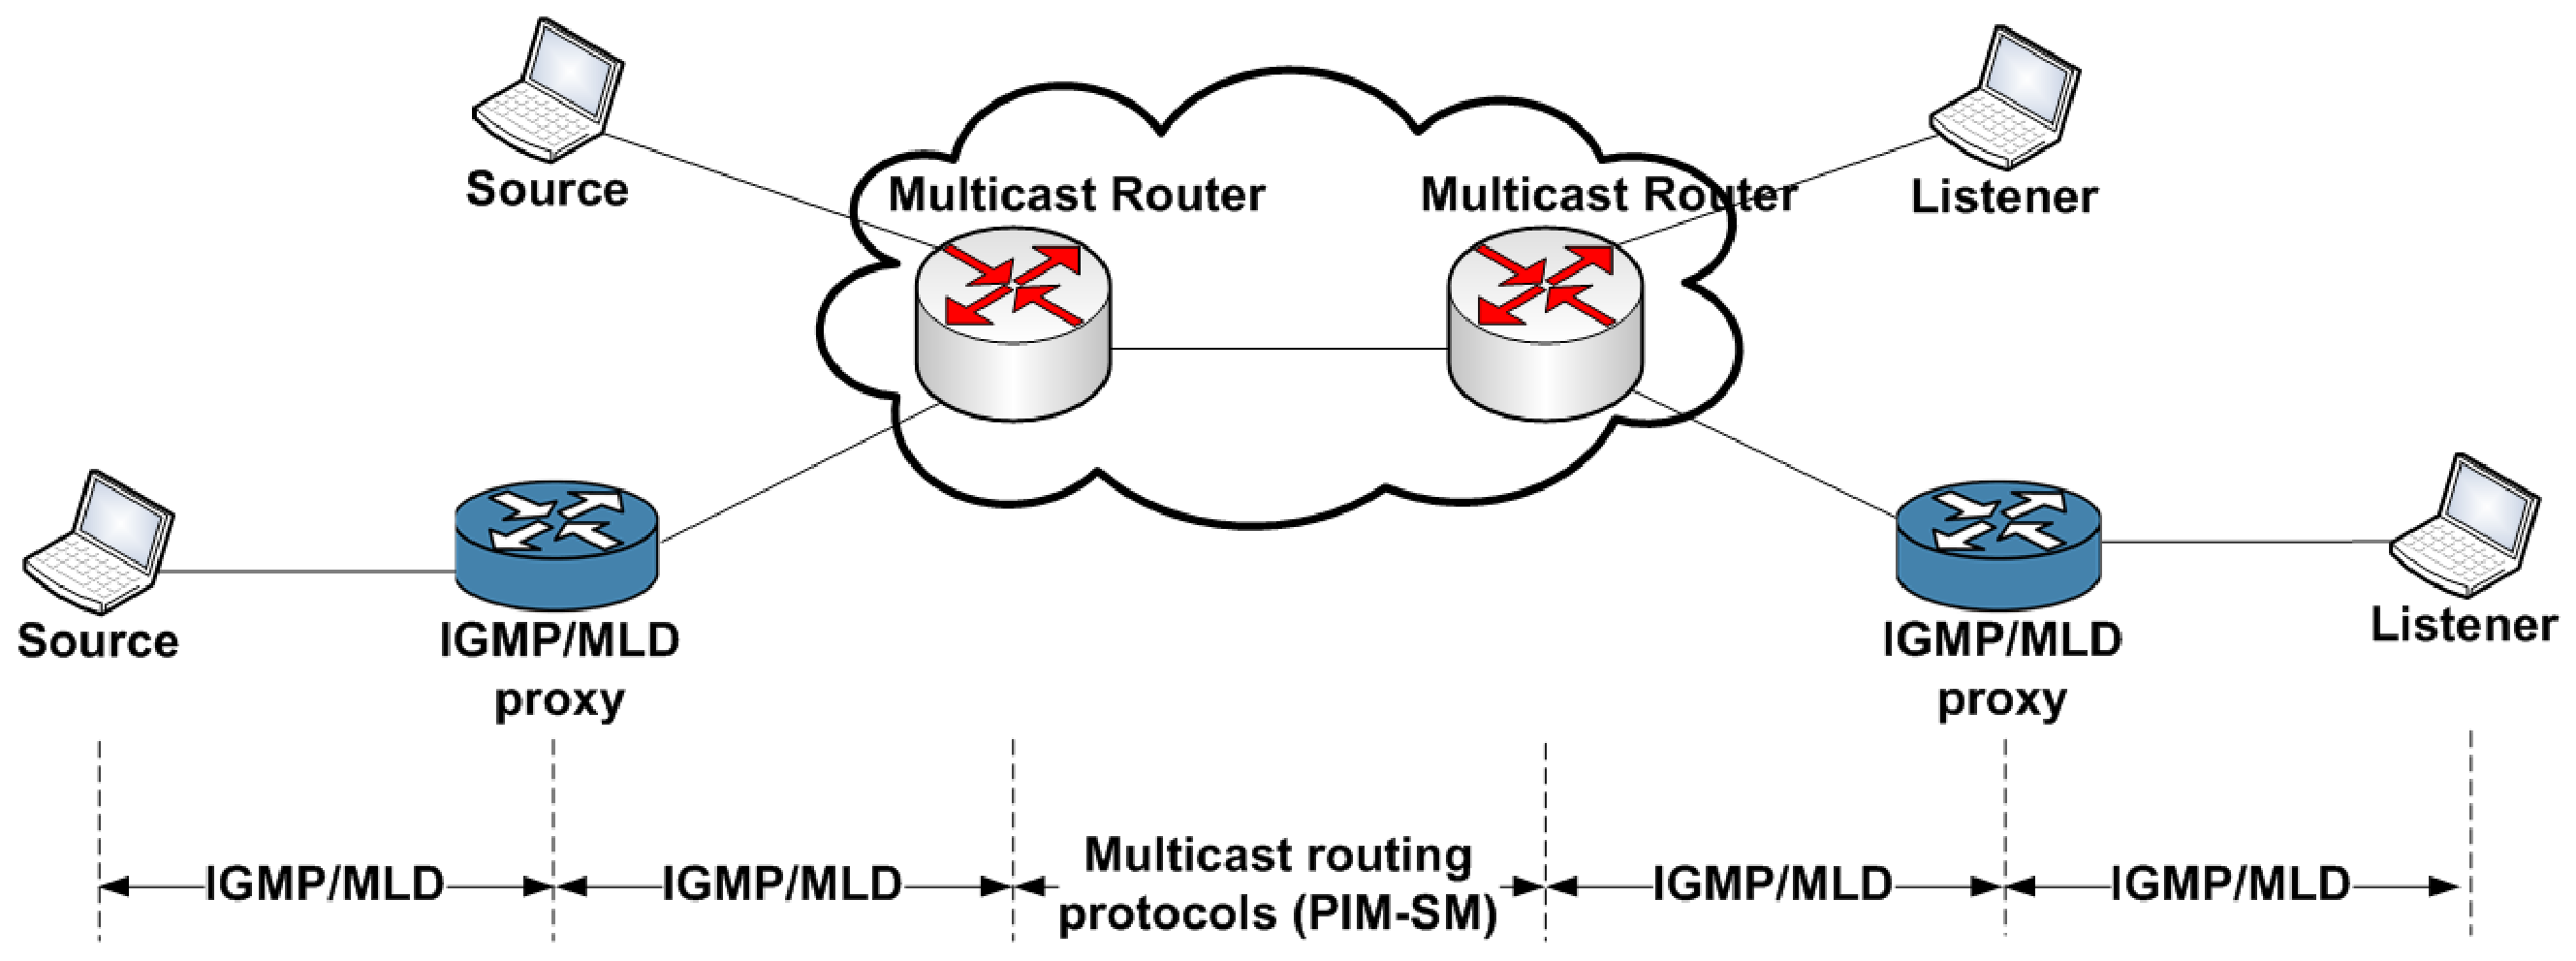
\includegraphics[width=0.85\textwidth]{./Part1/Chapter2/figures/c2_multicast_deployment.eps} 
    \caption[A multicast deployment scenario: from protocols point of view]{A multicast deployment scenario: from protocols point of view.}
     \label{fig:c2_multicast_deployment}
  \end{center} 
\end{figure}

In order to provide multicast service, two groups of protocol need to be deployed: multicast group membership protocols and multicast routing protocols. The multicast group membership protocols enable hosts to dynamically join/leave the group as well as make multicast routers (MR) aware of the interested receivers and manage their subscriptions. The multicast routing protocols enable a collection of MRs to build distribution trees to deliver the multicast traffic from sources to all the members of a multicast group.
The multicast group membership protocols, depending on IP version, are Internet Group Management Protocol (IGMP) \cite{IGMPv3} for IPv4 and Multicast Listener Discovery (MLD) \cite{MLDv2} for IPv6. 

Regarding the multicast routing protocols, each protocol uses its multicast routing algorithm to build the multicast delivery tree. There are many multicast routing protocols such as Distance Vector Multicast Routing Protocol (DVMRP) \cite{DVMRP}, Multicast Open Shortest Path First (MOSPF) \cite{MOSPF}, Core Based Tree (CBT) \cite{CBT,CBTv2}, Protocol Independent Multicast – Dense Mode (PIM-DM) \cite{PIM_DM}, and Protocol Independent Multicast – Sparse Mode (PIM-SM) \cite{PIM_SM}. 
In this thesis, the considered multicast routing protocols are PIM-SM and the enhanced version of PIM-SM for source specific (PIM-SSM \cite{PIM_SM}). To avoid deploying a full-stack MR inside a given network due to its implementation and operational costs, IGMP/MLD proxy \cite{MLD_proxy} which performs membership management, acts as a multicast Querier for its subnet and as a host for an upstream proxy/MR, is introduced. 

Fig.~\ref{fig:c2_multicast_architecture} and Fig.~\ref{fig:c2_multicast_deployment} show an example of a multicast deployment scenario from architecture and protocol point of view, respectively. As seen in Fig.~\ref{fig:c2_multicast_architecture}, multicast sources/listeners can be a mobile node or a fixed node. The multicast traffic is routed from the sources to the listeners via the intermediate MRs and/or MLD proxies. 

\subsection{IP Multicast Applications}
Taking advantages of multicast, various applications which can be classified into different groups following different criteria can be deployed. In terms of multicast model, the multicast applications can be placed into three main categories, as stated in \cite{multicast_applications,multimedia_multicast}:
\begin{itemize}
\item One-to-many (a single source sending to a set of receivers):  A typical example is scheduled audio/video distribution (including Internet Protocol Television (IPTV), mobile TV, lectures, presentations, etc.). Also, the multicast application can be used to push media like news headlines, weather updates, sport scores and financial services. Software update also falls into this category. 
\item Many-to-many (multiple sources sending to a set of receivers): Applications such as audio/video conferencing, distributed online games, and collaborative environments, in which some or all the participants become sources, are examples of the many-to-many model. 
\item Many-to-one (multiple sources sending to a receiver): Many-to-one applications include resource discovery (e.g., service location and device discovery), data collection (monitoring applications, video surveillance), and so on.  
\end{itemize}

Following the service function, these applications fall into such groups as Mobile TV (live and interactive TV), Personal Broadcasting Service (PBS), Live Video Distribution (conferences, seminars, etc.), Multimedia Content Distribution (Video On-Demand), General Content Distribution (Data on Demand, Online Gaming), and Machine-to-Machine Distribution (e.g., Software distribution and navigation system updates) \cite{multicast_3g_networks}. 
 
 \subsection{Multicast Model}
At the time IP multicast was introduced, a \textit{host group} model supported both one-to-many and many-to-many group communication (referred as Any-Source Multicast, or ASM). However, this model is also one of the main barriers for the widely multicast deployment. It is due to the fact that there are several deployment issues of the ASM model such as multicast address allocation and management, lack of access control (leading to the denial of service attacks), scalability and service provisioning \cite{overview_SSM,SSM}.   

To promote the deployment of multicast, a new service model, the so-called Source-Specific Multicast (SSM), is introduced. The great advantage of SSM is the simplicity. SSM model also overcomes the limitation of ASM and is suitable for one-to-many applications. 
A range of multicast addresses (FF3x::/32 for IPv6) is reserved for SSM. In more details, SSM simplifies the multicast related mechanism by eliminating the need of the Rendezvous-Point Tree (RPT), RP, and Multicast Source Discovery Protocol (MSDP)\footnote{ The control plane for source discovery is now under the responsibility of receivers}. To cope with SSM model, the group management protocol is required to support source filtering as described in \cite{MLD_SSM}. Also, PIM-SSM \cite{PIM_SM}, as an extension of PIM-SM, is specified to handle a source-specific model.

\subsection{Group Management Protocols}
Multicast group membership protocols consist of two parts. The first part, namely multicast listener one, is used by hosts/routers to announce their interest in receiving traffic destined to a specified group with their neighboring MRs. 
The second part, multicast router one, is performed by the MRs to discover the presence of the interested hosts of a given group and to manage their subscriptions for each of their directly attached link. IETF defines two multicast group membership protocols, i.e., IGMP \cite{RFC1112, IGMPv2, IGMPv3} for IPv4 and MLD \cite{MLDv1,MLDv2} for IPv6. The current version of IGMP (IGMPv3 \cite{IGMPv3}) and MLD (MLDv2 \cite{MLDv2}) share the same functionality. In this thesis, only MLDv2 is considered since we focus on the IPv6 network. The interaction between the two parts is done by using MLD messages. 

From a multicast listener point of view, when the upper-layer protocols or application programs ask the IP layer to enable the reception of multicast traffic from a specific multicast address, a node will send an MLD Report message to its MR to join this group. The MR then joins the multicast group (if necessary) and forwards the multicast packets to the subscribed nodes. The MLD Report is also used to reply to the general queries which are periodically sent by the MR to learn about the multicast subscription information from an attached link. In addition, if the listening state of a node changes, the node will immediately report this change via a State Change Report message.

From an MR point of view, the MR uses MLD to learn, for each of its directly attached links, which multicast addresses and which sources have listeners interested on that link (to support SSM). Thus, the router only needs to know whether there is at least one group member per network interface which is interested in receiving the multicast traffic of a multicast group, or not. However, the router can maintain the detailed subscription information regarding the multicast addresses, their corresponding subscribed hosts, and the associated network interface by means of the explicit tracking function \cite{explicit_tracking}. Enabling the explicit tracking function can help reduce the multicast-related issues in a wireless environment such as signaling overhead and leave latency. 

The basic operations of MLD are briefly described as follows:
\begin{itemize}
\item One MR in a subnet, the so-called Querier \cite{MLDv2}, periodically sends MLD General Query messages onto the link to build and update the multicast membership state of all multicast routes on this link. 
\item Nodes respond to these queries by sending a Current State Report message indicating their group memberships to all MLDv2 routers on the link. Whenever their listening state changes, they report these changes to the routers via a State Change Report message. 
\item All routers, upon the reception of the Report messages, update the memberships state on the link. If the Querier receives an MLD State Change Report indicating that the node desires to stop listening to a particular group, the Querier will make a query for the presence of other listeners subscribed to this group using a Multicast Address Specific Query, before deciding to stop forwarding multicast traffic for this group. Similarly, the Multicast Address and Source Specific Query is used to learn the membership state of a specified multicast address with specified source address. 
\item If a router does not receive a Report message for a particular group for a period of time, it will assume that there are no more members of the group on the link and can stop forwarding the multicast packets for this group. 
\end{itemize}

\subsection{Multicast Routing Protocols}
IP multicast does not require a source sending to a given group to know about the receivers of the group, instead it is based on the multicast delivery trees to deliver the multicast packets. Multicast routing protocols are responsible for building the multicast delivery trees and forwarding the multicast packets along the trees to the appropriate receivers. Various multicast routing protocols, according to the type of the multicast tree they build, can be grouped into two categories: a source-based tree and a share tree. 

The source-based tree (or shortest-path tree) protocols are based on the shortest path towards the source to build a tree to minimize the path cost from the source to each receiver. Thus, such a separate delivery tree is built for each multicast source of a given group. In this case, the multicast packets will be delivered along a shortest-path tree from the source to the members of multicast group in order to meet the objective of a low-delay multicasting \cite{Deering_88}. Protocols such as DVMRP, MOSPF, PIM-SSM and PIM-DM use this kind of multicast delivery tree. 

For example, DVMRP is the first multicast routing protocol proposed by S. Deering \cite{Deering_88}. DVMRP is a flood-and-prune protocol in a sense that the source floods the multicast packets to the entire domain and the routers which do not have multicast listener for this group send a prune message to stop forwarding packet to them. In more details, the packets that do not arrive at a router on the appropriate interface (the interface from which the router could forward a unicast packet to the source following the shortest path) are ignored. Otherwise, they will be forwarded to all, except the incoming interface. Based on IGMP protocol, the leaf routers which do not have multicast listener for this group prune back to the spanning tree. However, the multicast packets need to be re-flooded to detect the new listeners. As a result, the prune messages need to be sent periodically to remove the unnecessary links along the shortest path tree towards the source. All together, it leads to the scalability issue.  

There is another type of algorithm, the so-called Shared Tree (or Core-based Tree) where a single tree is shared by all the sources of the same multicast group. In other words, the multicast traffic for each group is sent and received over the same delivery tree, regardless of the source. It is achieved by introducing a core router, the so-called Rendezvous Point (RP) which is a pre-defined router. The MR may statically store the address of RP or discover the address during the bootstrap phase \cite{PIM_SM}. When a source transmits a packet to a multicast group, the packet is first sent to the RP which then forwards the packet along the reverse shortest path tree (towards the RP) to reach all the listeners. Moreover, each edge router which desires to receive the multicast traffic has to join the tree by sending an explicit \textit{Join} message towards the RP. Based on that, the multicast delivery tree is built. Comparing to the previous algorithm, CBT is better regarding network bandwidth since it does not require the multicast packets to be periodically forwarded to all MRs in the internetwork. Protocols such as CBT and PIM-SM use the core-based tree. 

Additionally, the flooding mechanism is suitable for the case where the members of the multicast group are densely distributed across the network. These protocols using it as a distribution mechanism are called dense-mode protocols. On the contrary, in the widely distributed multicast environments where the group members are spread sparsely across the network, the flooding mechanism may cause a waste of bandwidth and performance issues. As a result, CBT with the explicit join mechanism is more suitable. The corresponding routing protocols are called the spare-mode ones. 

\subsubsection{Protocol Independent Multicast-Spare Mode/Source-Specific Mode}

The name of Protocol Independent Multicast (PIM) derives from the fact that PIM does not have its own unicast routing protocol, instead it relies on the existing unicast routing protocols to build a separate multicast forwarding table. PIM-Spare Mode (PIM-SM), a spare-mode protocol, is the most widely used multicast routing protocol. PIM-SM is a dual-stack protocol for both IPv4 and IPv6. However, in the scope of this thesis, we focus on IPv6 part of this protocol which uses both the source-based and the shared-tree to deliver the multicast traffic. 

In PIM-SM, a RP plays the role of a core of the multicast delivery tree in a sense that the source sends the multicast packet to the RP. When a listener wishes to receive multicast traffic from a group, it sends an MLD Report to its default MR (designated router or DR) which then joins the multicast delivery tree on behalf of the listener. As a result, the existence of the sources and the listeners are independent of each other. The detailed operation of PIM-SM is described as follows.

The PIM-SM operations consist of three phases as described in Fig.~\ref{c2_pim_operation}. In the phase one (see Fig.~\ref{fig:c2_pim_p1}), a multicast listener expresses its interest in receiving multicast traffic  destined for a given group by sending an MLD Report to its DR. The DR then sends a PIM Join message towards the RP for that group. Since the multicast traffic can arrive from any sources, the Join message is denoted as (*, G) Join. The MRs on the path towards the RP of the (*, G) Join establish the multicast tree state for group G. Therefore, a multicast delivery tree with the root at the RP is constructed for group G, called RP Tree (RPT). Since the RPT is shared by all the sources, it is considered as a shared tree. From a multicast source point of view, the source can start sending data packets destined for a group at anytime. The source's DR, upon receiving the multicast packets, unicast-encapsulates them and sends them directly to the RP (as known as the registering process). The RP, on the reception of the encapsulated packets, decapsulates them and forwards them natively following the multicast forwarding state onto the shared tree. The multicast packets are then replicated by the intermediate routers and reach the listeners. The encapsulation packets are called the PIM Register packets. 
\begin{figure}[h!]
\centering
\subfloat[]{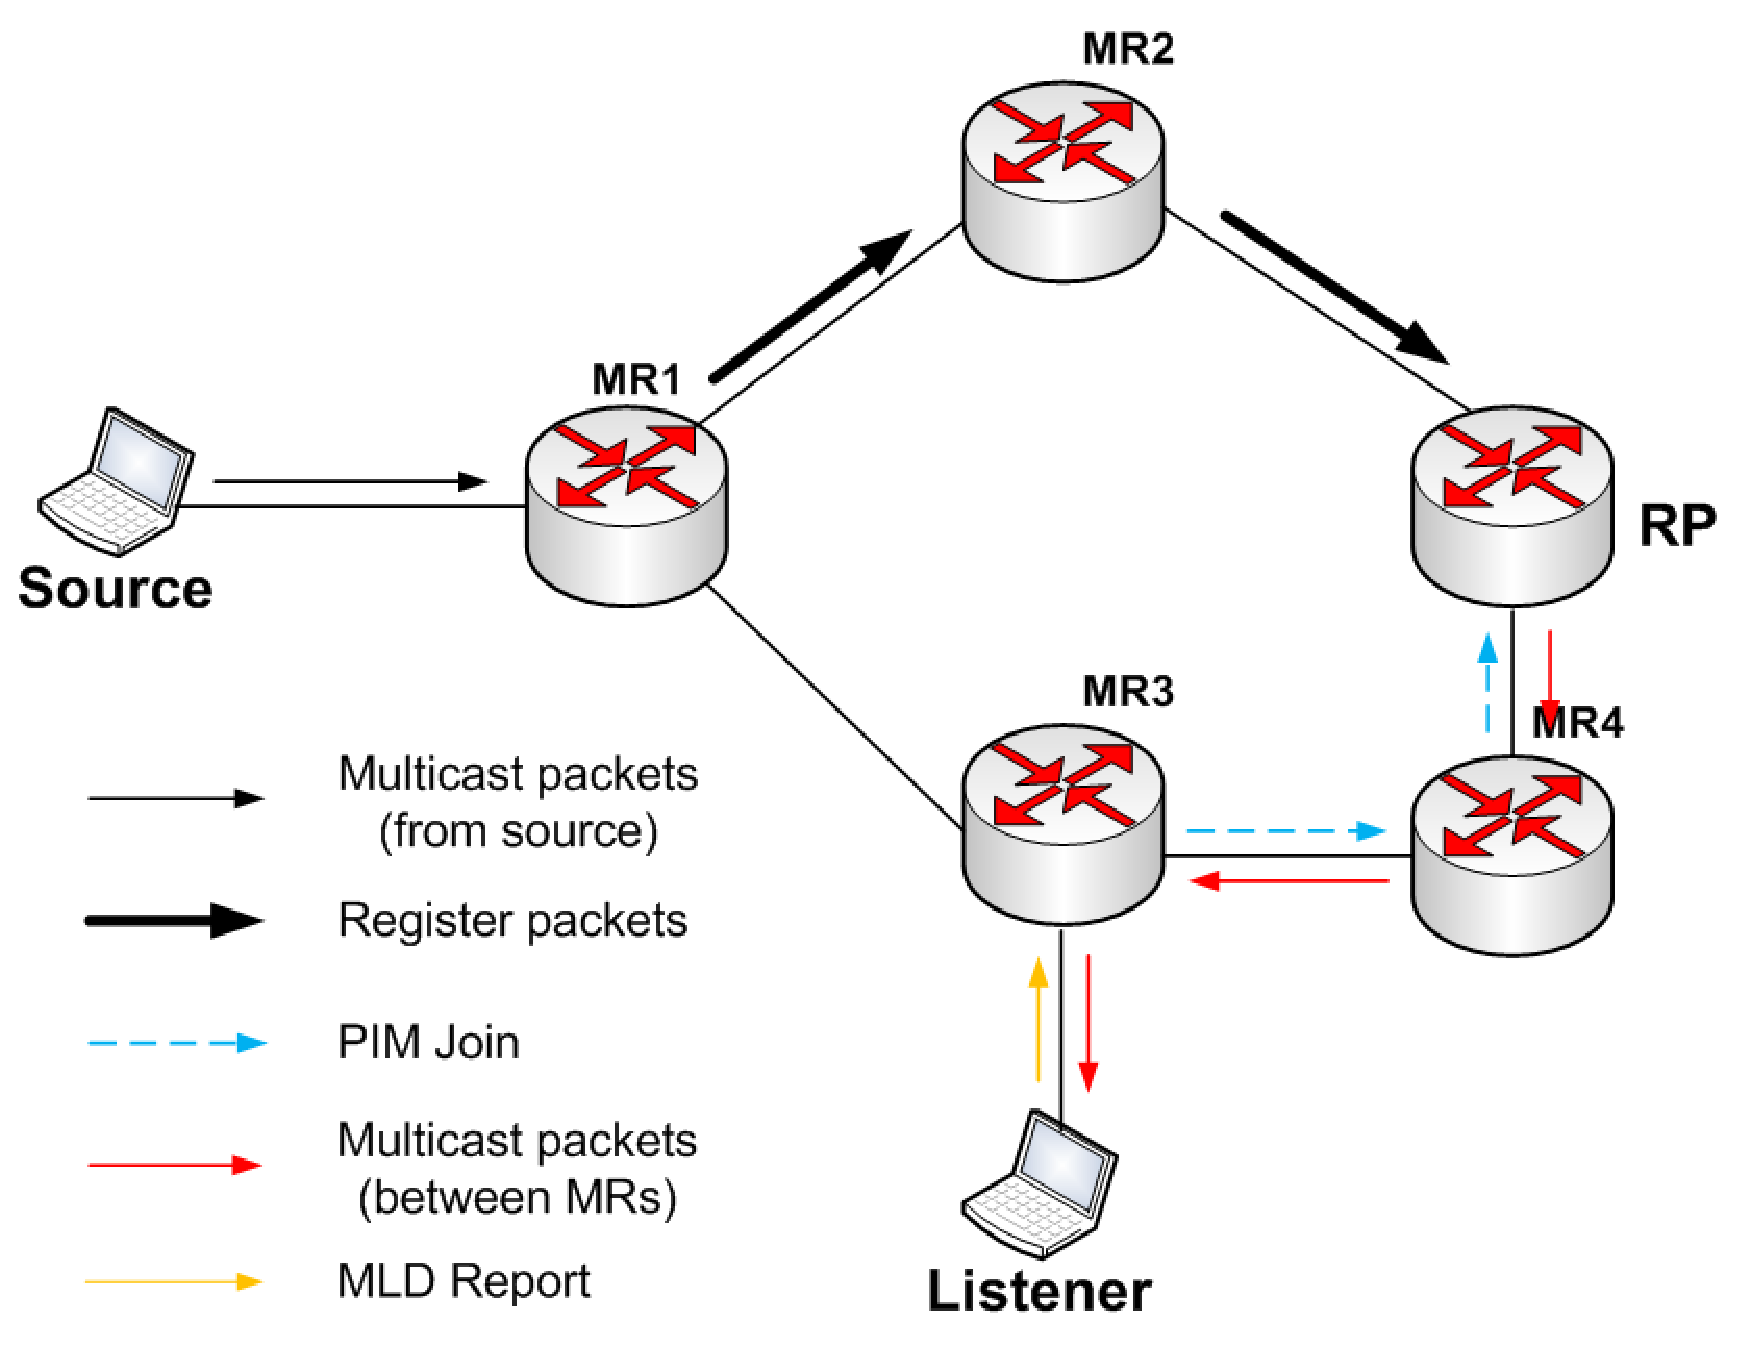
\includegraphics[width=0.47\textwidth]{./Part1/Chapter2/figures/pim_p1.eps} \label{fig:c2_pim_p1}}\,
\subfloat[]{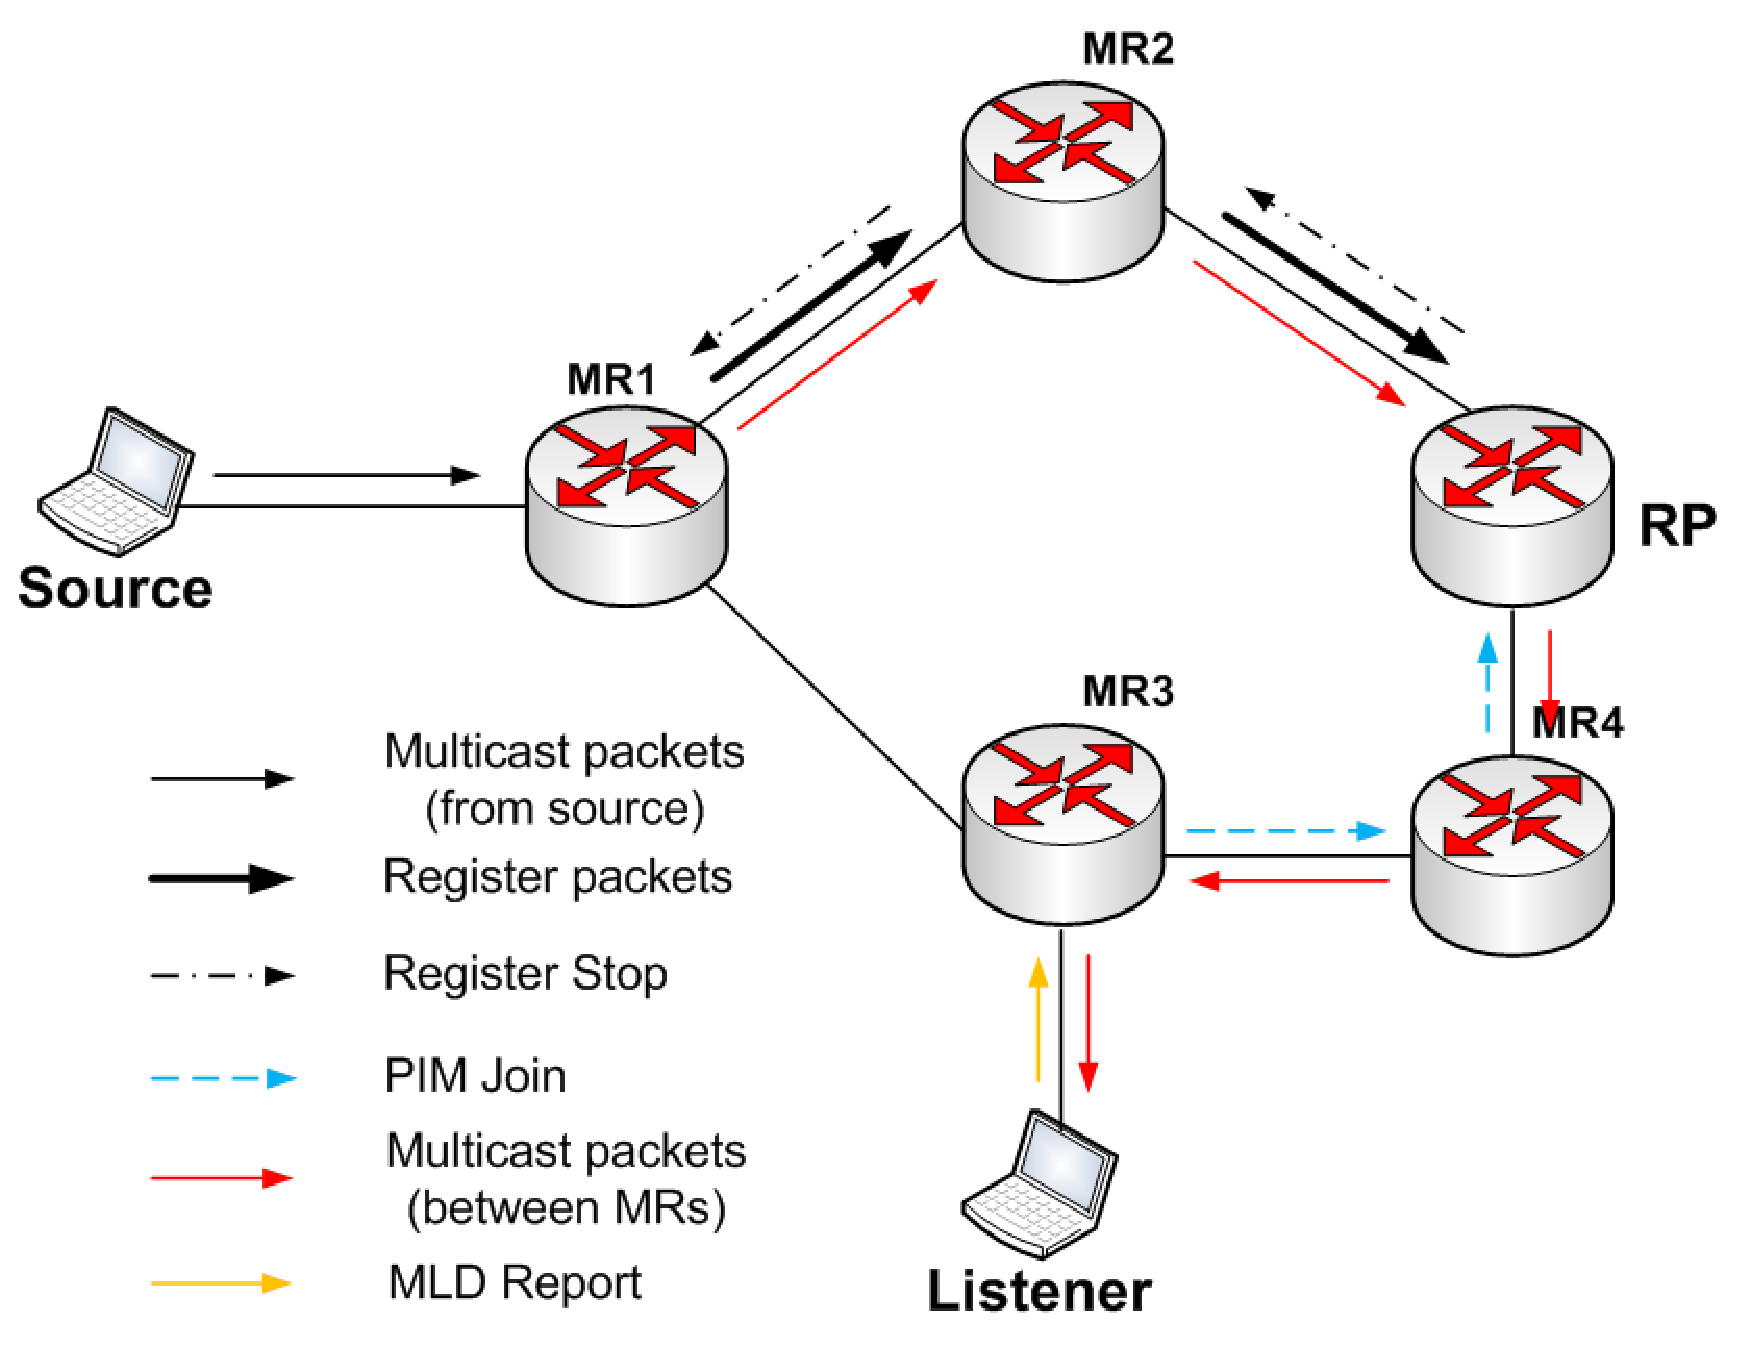
\includegraphics[width=0.47\textwidth]{./Part1/Chapter2/figures/pim_p2.eps}\label{fig:c2_pim_p2}}\,
\subfloat[]{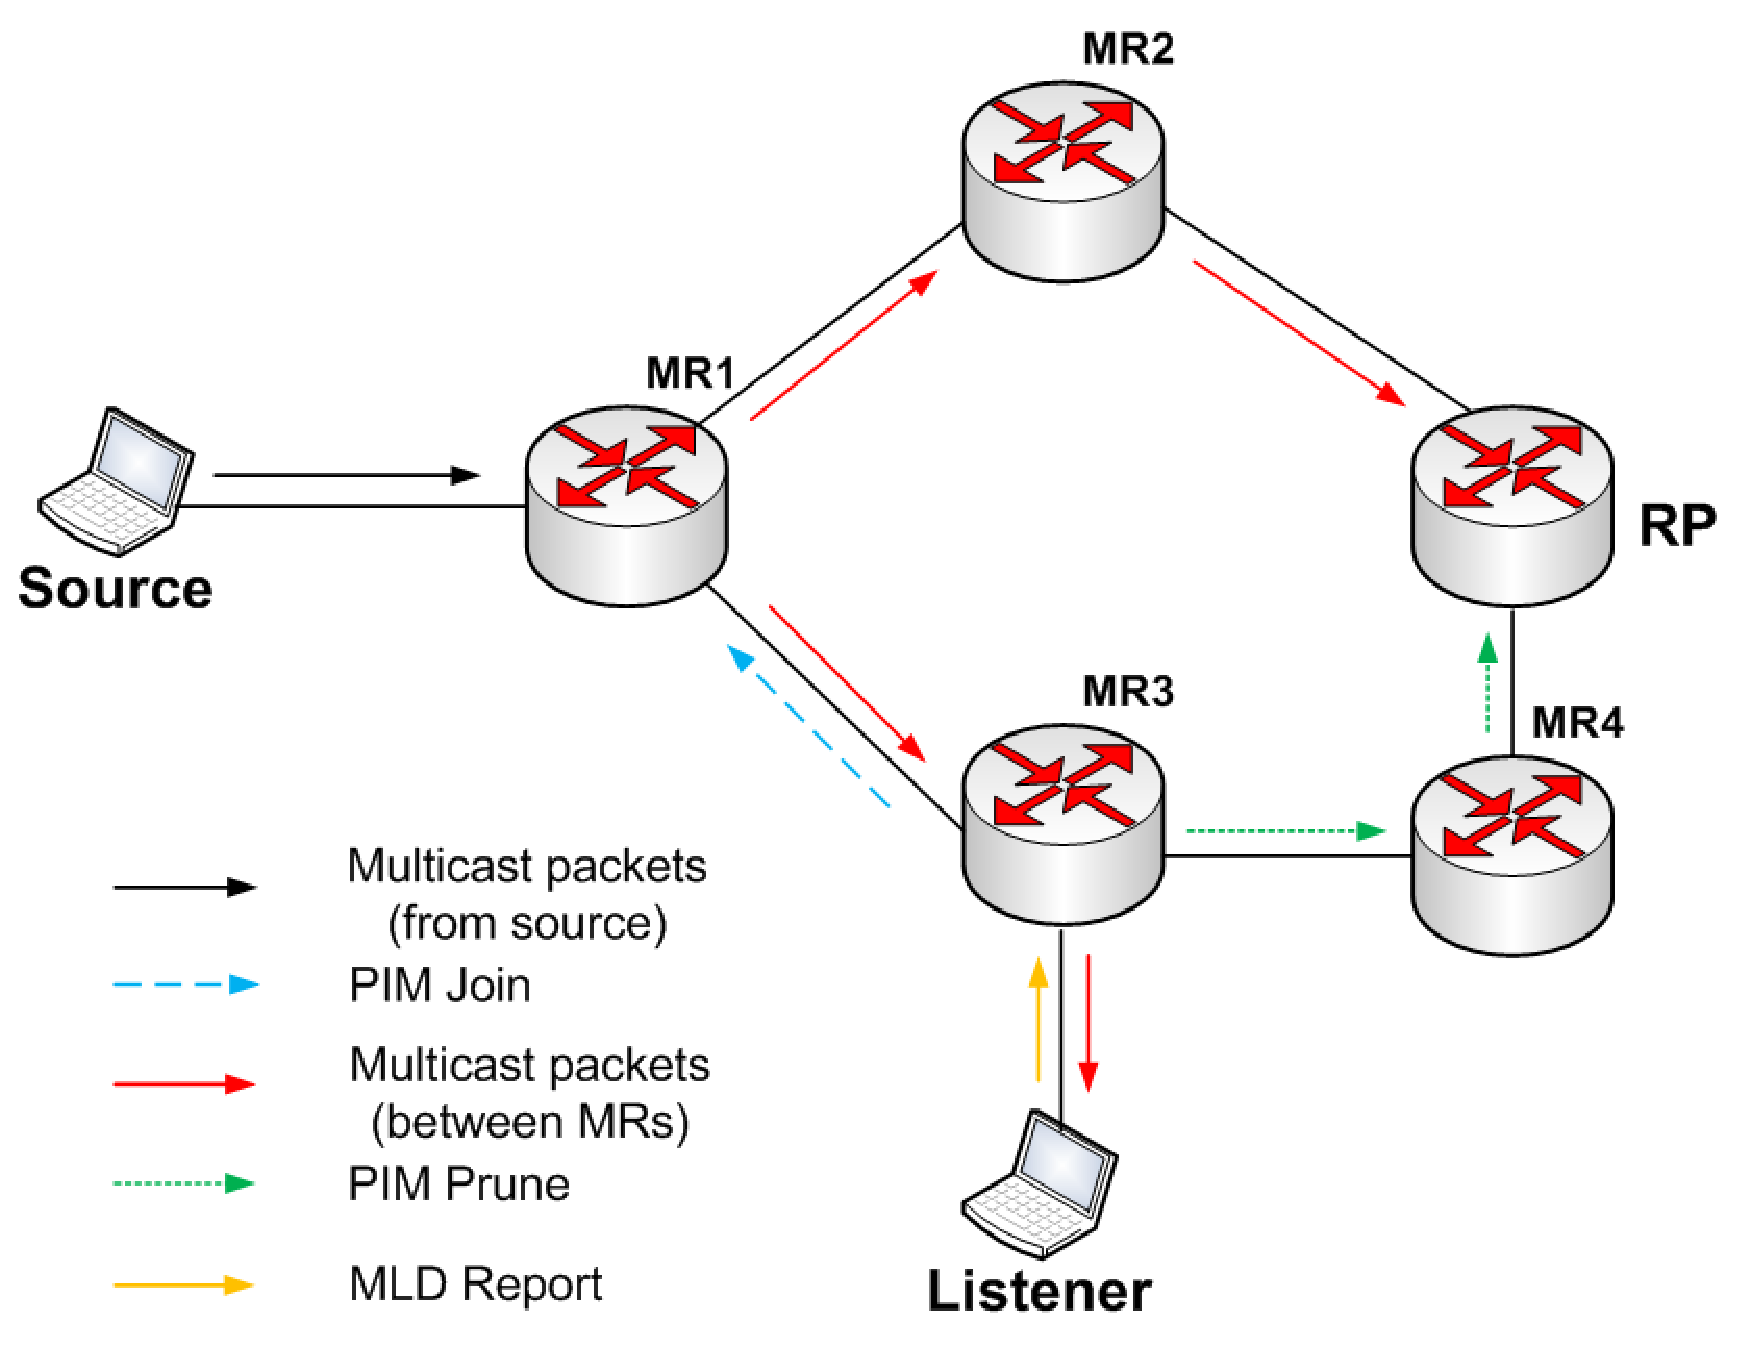
\includegraphics[width=0.47\textwidth]{./Part1/Chapter2/figures/pim_p3.eps}\label{fig:c2_pim_p3}}
\caption[The operations of PIM-SM]{PIM-SM operations: (a) phase 1, (b) phase 2, (c) phase 3.}
\label{c2_pim_operation}
\end{figure}

In the phase two (see Fig.~\ref{fig:c2_pim_p2}), after receiving the PIM Register packets from a source S, the RP may decide to switch to a native multicast forwarding by sending a (S, G) Join towards the source S. Similarly, the (S, G) multicast tree, which is the shortest-path tree towards the source S, will be established. In the meantime, the data packet will continue being encapsulated to the RP. As soon as the multicast packets arrive natively at the RP, the RP sends a Register-Stop message to inform the source's DR to stop encapsulating the packets. At the end of this phase, the traffic will be routed natively from source S to the RP, and then along the shared tree to the listeners.      

Fig.~\ref{fig:c2_pim_p3} illustrates the PIM operations in the phase three. As the traffic passes through the RP, it is usually not an optimal path from the source to the listener. Thus, the listener's DR may send a (S, G) Join towards the source to switch to the shortest path tree. Similarly, after receiving the multicast packets from the source, the listener's DR sends a Prune message to the RP (known as  (S, G, rpt) Prune) to prune the unnecessary routes. At the end of this phase, the multicast traffic is routed following a shortest-path tree from the source S to the listener. 

The SSM model can be enabled at a PIM-SM router by using a subset of the PIM-SM protocol mechanisms. In more details, from an MR point of view, only (S, G) Join/Prune messages are generated by the router, and no (*, G) and (*, G, rpt) Join/Prune messages are generated. The packets related to (*, G) or (S, G, rpt) state should be ignored. PIM-SSM is backward compatible with PIM-SM, that means the router can only implement a subset of PIM-SM for SSM support. 
 
\subsection{IGMP/MLD Proxy}
The operators, in some cases, may not desire to deploy the multicast routing function on the routers inside a given network due to the hardware, the implementation and operational cost of an MR. In this case, IGMP/MLD proxy (is referred as MLD proxy, from now on) \cite{MLD_proxy}, as a lightweight protocol compared to the complicated multicast routing protocols such as PIM and DVMRP, can be used to simplify the design and implementation of the router. It should be noted that MLD proxy only works in a single tree topology as can be seen in Fig.~\ref{fig:c2_multicast_architecture}. This proxy performs the router part of MLD protocol on its subnet and the host part on its upstream interface. In other words, the MLD proxy function allows an intermediate node to appear as an MR to the downstream hosts and as a host to the upstream MRs. The MLD proxy device maintains a database as a multicast membership. The MLD proxy will forward the multicast packets arriving from an upstream interface to all the downstream interfaces that have the subscription information of this group. Also, if a packet arrives at the proxy from a downstream interface, it will be forwarded to the upstream interface and to all the downstream interfaces that have the subscription information of this group except the incoming one. 

\section{IP Mobility Management}\label{c1:IP_Mobility}

Nowadays, the mobile data services have become an essential part of many consumers' lives \cite{cisco_forecast,data_services}. 
So far, the users have been using their mobile devices (e.g., smartphones and tablets) not only for personal life (e.g., making voice/video calls, sending email, watching video/TV, playing online games, and so on) but also for work (general and job-specific work applications such as multimedia conferencing, and distance learning, etc.) on a regular basic \cite{cisco_service,morgan_stanley, mobile_2010}. As a result, the mobile data traffic has been almost doubled each year during the last few years \cite{ericsson}. This trend is expected to continue in the upcoming years, especially with the deployment of 4G networks. The widely usage of mobile data services has been driven by the variety of different reasons such as: the increasing number of mobile devices which become more and more powerful and intelligent, the enhancement of wireless access technology in terms of coverage, speed and quality, as well as the explosion of mobile applications \cite{ericsson}. The mobility of the devices puts a new requirement on the mobile operators to provide connectivity anywhere and at anytime. Moreover, providing consistent and seamless services is required for satisfying user's expectations and fulfilling even highly application requirements in terms of service disruption on the move \cite{seamless}. 

In all-IP mobile networks, IP mobility is a crucial concept to meet the demand of ubiquitous Internet connectivity as well as new service requirements such as seamless handover across heterogeneous networks, consistent quality of experience and stringent delay constraints. IP mobility can be handled at different layers of protocol stack ranging from the link layer to the application layer \cite{RFC6301, survey_mobility_management, mobility_handoff_management}. The link layer mobility management protocols use the underlink information for mobility-related procedures when the MN roams among different physical points of attachment while keeping its layer 3 attachment (preservation of the IP address). The transport layer mobility management protocols  \cite{transport_layer_snoeren, transport_layer_Atiquzzaman} provide an end-to-end mobility support without requiring to change the network layer infrastructure. Regarding the mobility protocols at the application layer, the most well-known protocol, Session Initiation Protocol (SIP) \cite{SIP_mobility,SIP_application_layer}, provides an end-to-end mobility management framework, which does not depend upon the network entities (e.g., HA) and can be deployed by any third-party application service providers. Due to the fact that most of the existing mobility management protocols are located at the network layer (since a network layer IP mobility is transparent to the upper layers as well as the applications \cite{L3_mobility_management, mobility_handoff_management}), we focus on these protocols in our thesis. 

Again, the mobility management protocols at the network layer can be classified according to different criteria such as the mobility range (micro- and macro-mobility) and the mobile host signaling (host- and network-based mobility) \cite{RFC6301,  survey_mobility_management, mobility_survey,mobility_handoff_management}. Regarding the mobility range, the mobility management can be categorized into two types: the macro-mobility and the micro-mobility. The macro-mobility (global mobility or inter-domain mobility) refers to the mobility between different domains (with different architectures and access technologies) over a large area. MIPv6 and Host Identify Protocol (HIP) \cite{HIP} fall in to this category. On the other hand, the micro-mobility (or intra-domain mobility) is referred as a mobility between different cells/subnets inside a single administrative domain. Some examples of micro-mobility protocol are HMIPv6, FMIPv6, and PMIPv6. Considering the mobile host signaling, the host-based mobility protocols such as MIPv6 and Dual Stack Mobile IPv6 (DSMIPv6) \cite{DSMIPv6}, require the host to participate in mobility-related signaling process. On the contrary, in the network-based mobility, the network entities handle the mobility process on behalf of the host. 

As stated above, the increasing penetration of the mobile devices, such as tablets and smart phones is generating a huge number of data traffic over the mobile networks. The mobile data traffic is expected to grow to 11.2 exabytes per month by 2017, a 13-fold increase over 2012 \cite{cisco_forecast}. Despite the increasing volume of traffic, the mobile data revenue per user is falling fast. Thus, the mobile network is evolving towards the flat network architecture in order to be able to cope with the huge amount of traffic and reduce data transmission costs. Examples of this trend are traffic offloading (e.g., LIPA/SIPTO) and content delivery network (CDN) \cite{DMM_issues}.
Considering the conventional IP mobility management (e.g., MIPv6, PMIPv6) which leverages on the centralized mobility management approach in a flat architecture, it raises several issues for the network operator like the inefficient use of network resources, poor performance, and scalability issues \cite{DMM_requirements, DMM_issues,DMM_problem_statement}. To overcome these problems, a novel concept, the so-called distributed (and dynamic) mobility management (DMM) has been introduced. A lot of research publications \cite{DMM_Bertin, PMIP_based_DMM_Giust, DMM_IETF_Lee, MIP_based_DMM_Condeixa, MIP_based_DMM_Hassan, DMM_analysis_Hassan} carried out the analysis on different DMM approaches and compared them with the conventional mobility managements in terms of signaling cost, packet delivery cost, handover delay, packet loss and end-to-end delay. The results from these analysis showed that DMM is a promising mobility management scheme. \\

In this section, we will briefly introduce a various IP mobility protocols ranging from the host-based to the network-based, from the centralized to  the distributed approach. We focus on MIPv6 as a typical example of the macro-mobility and host-based mobility; and PMIPv6 as an example of the micro-mobility and network-based mobility. Finally, DMM will be presented, mainly focusing on the network-based approach. 
 
 \subsection{Centralized Mobility Management}
\subsubsection{Mobile IPv6}
Mobile IPv6 (MIPv6) \cite{MIPv6} is the first mobility protocol standardized by the IETF for IPv6 networks. As a global mobility protocol, MIPv6 maintains the mobile node's reachability when it is away from home. It is done by introducing a central mobility, namely Home Agent (HA) located at the MN's home network, which is a topological anchor point of the permanent MN's IP address (Home Address or HoA). Using its home address, the MN can communicate regardless of its actual location in the Internet. When the MN is away from home, it may obtain a temporal IP address (namely care-of-address (CoA)) which can be used in the foreign network for routing purposes. This address identifies the current location of the MN. The MN then registers its current topological location (CoA) with its HA by means of Binding Update (BU)/Binding Acknowledgment (BA) messages. The HA keeps track of the MN's current location by maintaining a binding association between the MN's HoA and MN's CoA (namely Binding Cache Entry - BCE). A bi-directional tunnel is then established between the HA and the MN for redirecting packets from/to the current location of the MN. In more details, the HA, acting as a topological anchor point of HoA, intercepts the packets addressed to the MN and tunneled them to the MN's CoA. On the other direction, the packets from MN are tunneled to the HA, before forwarding to the CN. However, a relevant drawback of MIPv6 is a triangular routing in which the packets have to pass through the HA, which is a typically longer route. To tackle this issue, the Router Optimization (RO) mode in which the MN communicates directly with the CN without passing through the HA is introduced. However, MIPv6 introduces several security vulnerabilities e.g., authentication and authorization of BUs during the RO process \cite{MIP_RO}. 

Additionally, MIPv6, as a global IP mobility solution, may cause a  high handover latency (and packet loss) that could significantly affect the performance of the on-going sessions \cite{HO_comparison_Makaya, HO_comparison_Lee}. The high signaling load is also required \cite{HO_comparison_Makaya, HO_comparison_Lee}. Thus, it is not optimized to handle the micro-mobility management, where low-latency handover and low mobility-related signaling are essential. Various solutions have been proposed to improve the performance of MIPv6 such as Hierarchical Mobile IPv6 (HMIPv6) \cite{HMIPv6} and Fast Mobile IPv6 (FMIPv6) \cite{FMIPv6}. In HMIPv6, the Mobility Anchor Point (MAP) which is located at a local domain is introduced. Each MAP can be served as a local mobility anchor for a local domain. In this case, the mobile node sends BU messages to the local MAP rather than the HA when it moves inside a local domain. The MN sends BU message to the HA only when it moves between MAPs. As a result, the handover latency as well as signaling cost are reduced. On the other hand, FMIPv6 aims at reducing the handover latency and the number of lost packets. In this case, the handover is prepared in advance by using the lower-layer information, thus allowing the MN to configure a new CoA before it actually moves to the new subnet. As a result, the MN can use the CoA address immediately when it connects to the new subnet. The packets are also forwarded from the previous router to the new one, thus, reducing the number of lost packets. 

As a host-based mobility protocol, in MIPv6, the MN needs to perform the mobility-related signaling by means of location update procedure. Consequently, the MIPv6 protocol stack is required at the MN. It is the major obstacle for the deployment of MIP in the reality. For this reason, the network-based localized mobility management (NetLMM\footnote{NetLMM WG: http://datatracker.ietf.org/wg/netlmm/charter/}) is proposed to avoid the additional deployment in the MN so that the MN can be kept simple. Moreover, the complex security mechanism to authenticate the location update signaling can be avoided. In other words, the mobility can be transparently provided to all the legacy MNs. 

\subsubsection{Proxy Mobile IPv6} \label{section:PMIPv6}
Unlike MIP6 and its host-based extensions in which the mobility functions need to be deployed at both network and terminal, a new approach, namely network-based localized mobility management (NetLMM), enables the mobility support without the MN's evolving in the signaling process. In this case, the mobility procedures are handled by the network entities. Proxy Mobile IPv6 (PMIPv6) \cite{PMIPv6}, as an extension of MIPv6,  was standardized by the IETF as a network-based mobility management protocol. PMIPv6 provides the mobility support within a localized area, namely a Localized Mobility Domain (LMD) or a PMIPv6 domain. While moving inside a LMD, the MN remains its IPv6 address. Thus, from IP layer point of view, the MN is unaware of mobility. This is achieved by introducing the network entity called the Mobile Access Gateway (MAG), which performs the mobility-related signaling on behalf of the MNs attached to its access links. In PMIPv6, the LMA, similar to HA in MIPv6, is responsible for maintaining the MN's reachability state and forwarding traffic from/to the current location of the MN. MN's traffic is always encapsulated and tunneled between the MN's LMA and the corresponding MAG. Each LMD consists of several LMAs and multiple MAGs, as illustrated in Fig.~\ref{fig:c3_pmip_domain}.
\begin{figure}[h!] 
 \begin{center} 
 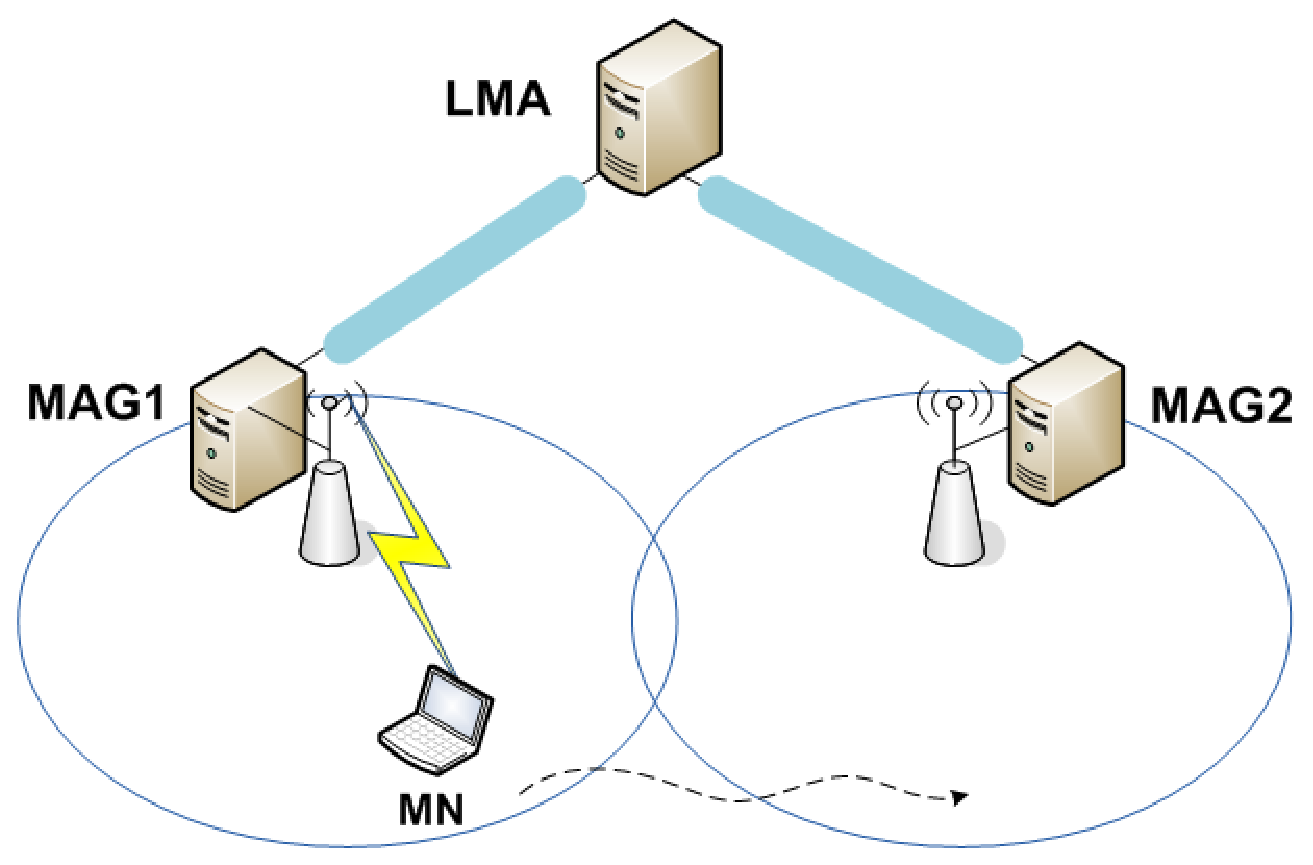
\includegraphics[width=0.50\textwidth]{./Part1/Chapter2/figures/c3_pmip_domain.eps} 
    \caption[The architecture of a PMIPv6 domain]{The architecture of a PMIPv6 domain.}
     \label{fig:c3_pmip_domain}
  \end{center} 
\end{figure}

Compared to MIPv6, PMIPv6 brings some benefits such as: (i) avoiding the complexity of the protocol stack at the MN; (ii) supporting mobility without the MN's involvement; and (iii) reducing tunneling overhead (over the air) and decreasing handover latency \cite{HO_comparison_Lee}.
\begin{figure}[h!] 
 \begin{center} 
 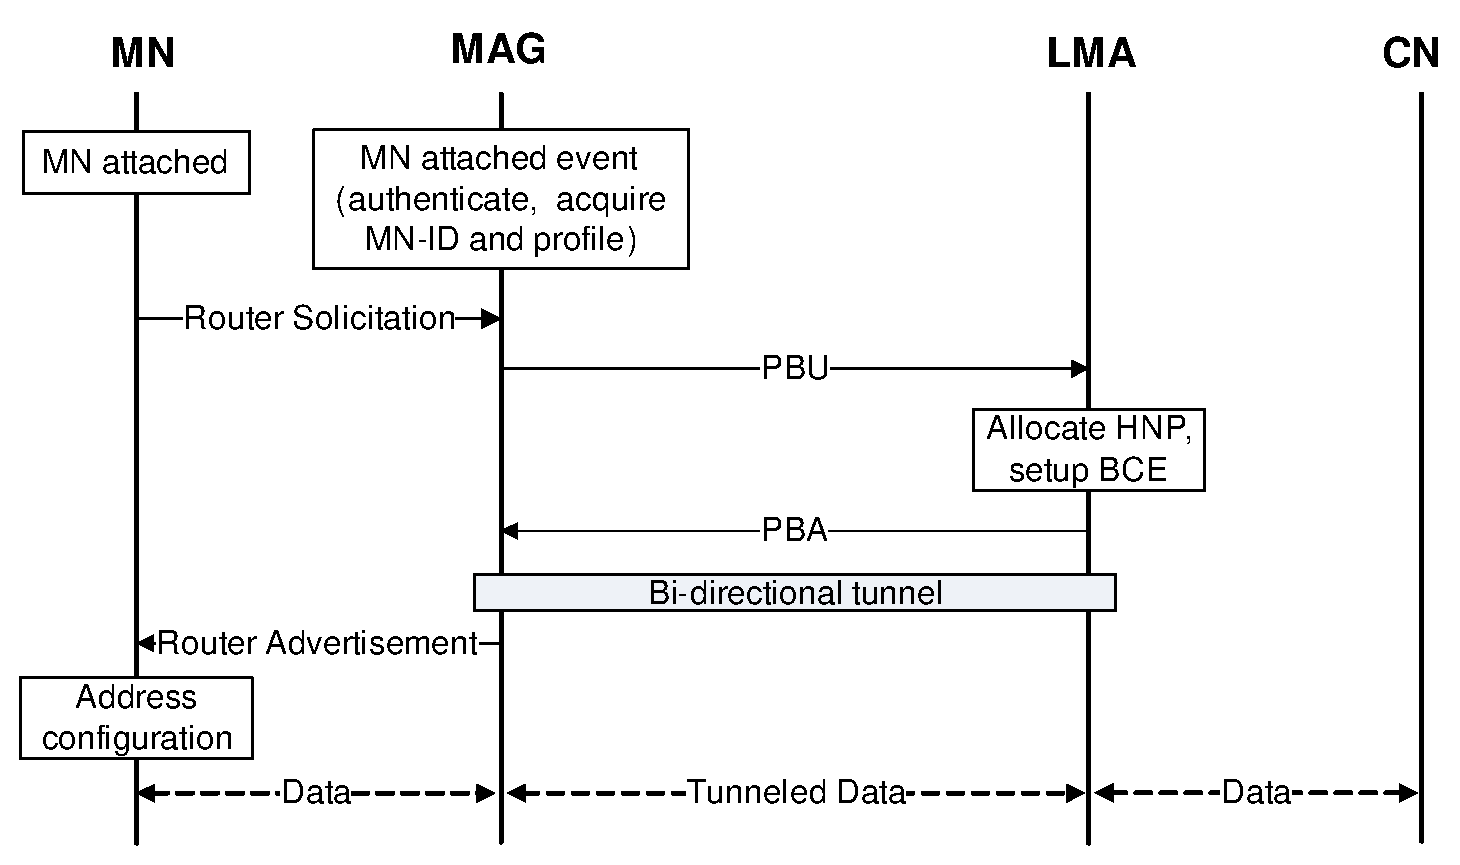
\includegraphics[width=0.60\textwidth]{./Part1/Chapter2/figures/c3_pmip_registration.eps} 
    \caption[Signaling when a mobile node attaches to the PMIPv6 domain]{Signaling when a mobile node attaches to the PMIPv6 domain.}
     \label{fig:c3_pmip_registration}
  \end{center} 
\end{figure}

The operation of PMIPv6 is briefly described as follows. Fig.~\ref{fig:c3_pmip_registration} shows signaling for the MN's initial attachment to a PMIPv6 domain. When an MN enters a PMIPv6 domain (attaches to a MAG), upon the detection of a new MN, the MAG fetches the MN profile, for example from an Authentication, Authorization and Accounting (AAA) server, and verifies if the MN is authorized for the network-based mobility service. Upon a successful authorization, the MAG sends a Proxy Binding Update (PBU) message to LMA to register a new MN. After receiving the PBU message, the LMA allocates a Home Network Prefix (HNP) to the MN, creates a BCE for this MN (including the MN's identifier (MN-ID, for example using the Network Access Identifier (NAI) \cite{NAI}, or its Media Access Control (MAC) address), HNP and the MN's MAG address (Proxy Care-of-Address or Proxy-CoA)). The LMA then replies by a Proxy Binding Acknowledgment (PBA) message including the allocated HNP. The MAG, on receiving the PBA, sets up the forwarding policy for the MN. A bi-directional tunnel is then established between the MAG and the LMA for redirecting the traffic from/to the MN. It is noted that the PBU/PBA messages are based on BU/BA messages with some specific extensions, respectively \cite{PMIPv6}. The MAG then sends a Router Advertisement (RA) message including the allocated HNP to the MN. The MN, based on the HNP, configures its address and can use it to communicate with a corresponding node (CN).
\begin{figure}[h!] 
 \begin{center} 
 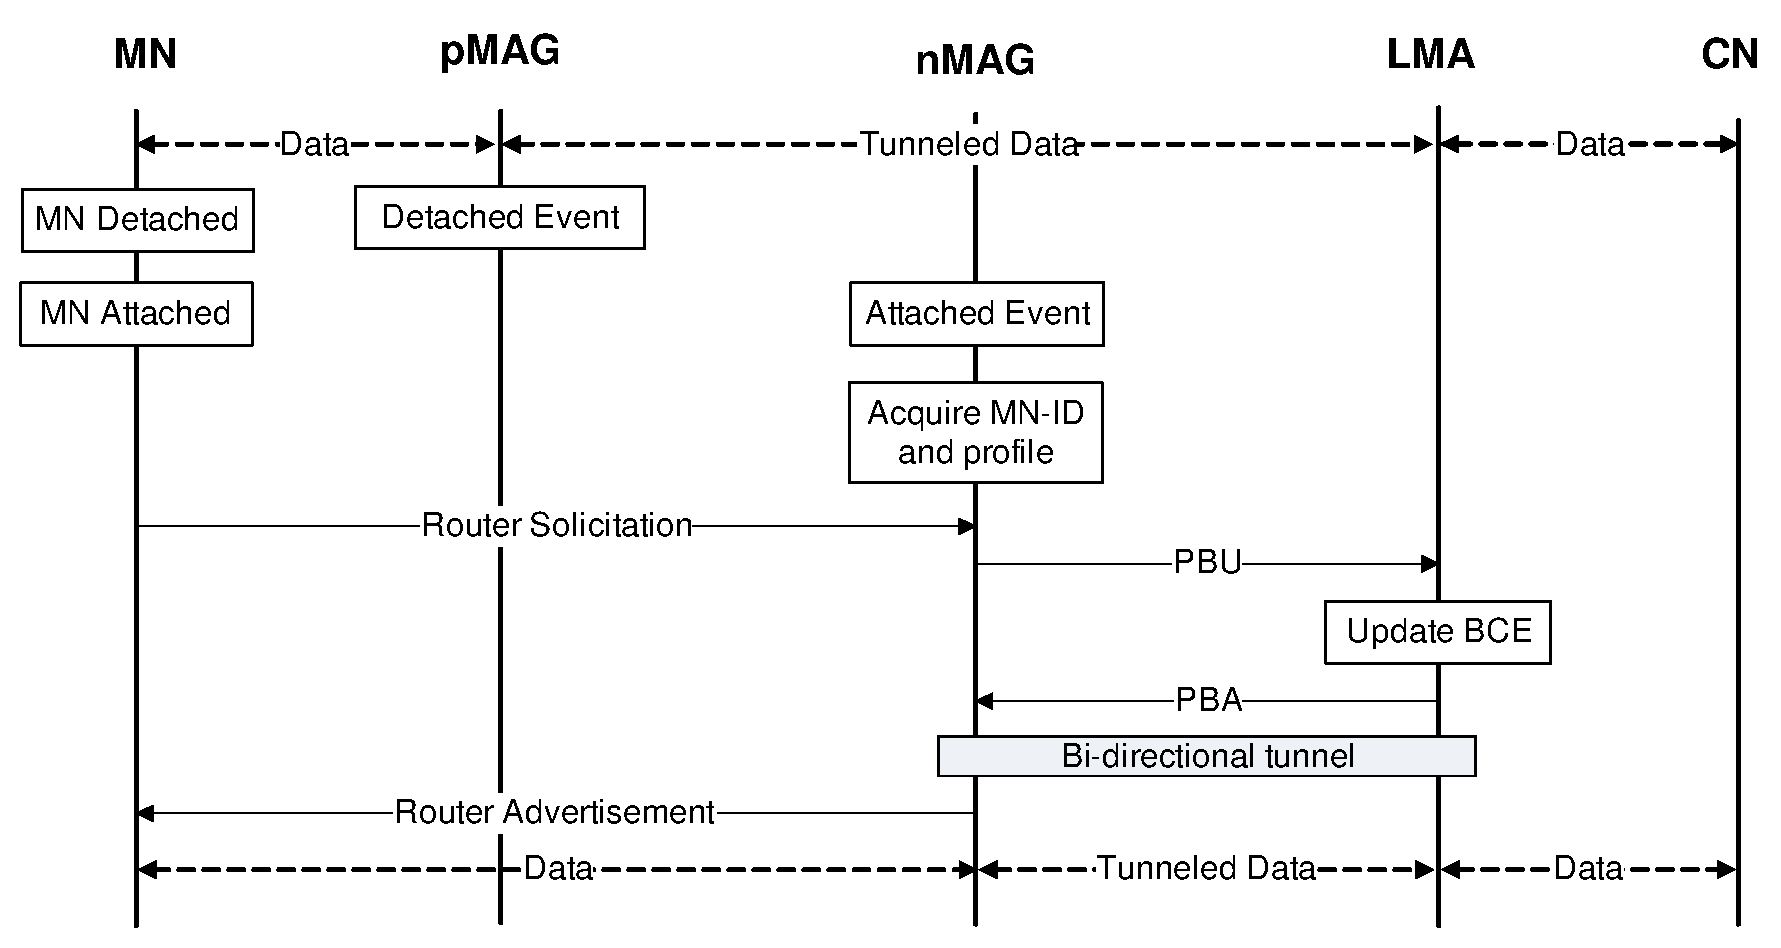
\includegraphics[width=0.68\textwidth]{./Part1/Chapter2/figures/c3_pmip_handover.eps} 
    \caption[Signaling when a mobile node performs a handover in the PMIPv6 domain]{Signaling when a mobile node performs a handover.}
     \label{fig:c3_pmip_handover}
  \end{center} 
\end{figure}

When the MN performs a handover from the previous MAG (pMAG) to a new one (nMAG), the similar process as in the registration step will be executed to update the MN’s current location at the LMA (see Fig.~\ref{fig:c3_pmip_handover}). In this case, the nMAG obtains the same HNP prefix for this MN and can emulate the MN’s home network (through sending RA messages with the same HNP). As a result, the MN is not aware of the mobility and continues to use the same IP address as before. Moreover, the link shared with a given MN of all the MAGs in the domain should be configured with the same link local address to make sure that the MN does not detect link changes as well as avoid the potential address collision issue \cite{PMIPv6} during the handover process.

Similar to FMIPv6, Fast Handovers for PMIPv6 (FPMIPv6) \cite{FPMIPv6} provides a fast handover mechanism for PMIPv6 in order to minimize the handover latency and the packet loss. Again, a bi-directional tunnel is established between the previous MAG and the current one to forward the packets to/from the MN. Also, the MN should provide information about the target network to the pMAG through L2 signaling. However, it inherits potential risks of erroneous movement and out-of-order packets delivery problem from FMIPv6

\paragraph{Extensions to PMIPv6}
Typically, the performance of a mobility management protocol is measured using such well-known metrics as signaling cost, handover latency, and packet loss. The signaling cost consists of the location update cost and the packet delivery cost. Handover latency is defined as the total time needed to complete the handover procedures. During this time, the MN cannot send or receive any packets. The handover latency typically consists of layer 2 handover duration and layer 3 one. The packet loss is the amount of lost packets originated from or sent to an MN during its handover. 

Various papers have been proposed which aim at improving PMIPv6 in terms of handover latency and signaling cost. In \cite{pmip_paging_Hong, pmip_paging_Lee}, the authors applied the paging technologies to PMIPv6 to reduce the location update signaling cost for the mobile host in the idle mode. In \cite{pmip_handover_latency_Kang}, the authors used the Neighbor Discovery (ND) message of IPv6 to reduce the handover latency and packet buffering at the MAG. In this case, the pMAG sent the MN's profile to the neighbor MAGs through ND message. Similarly, in \cite{pmip_handover_latency_Kim}, the pMAG sent the MN’s HNP to the adjacent MAGs in advance in order to perform the address configuration quickly after MN’s handover. In \cite{pmip_handover_latency_Magagula}, the improvement on handover latency was achieved by using the IEEE 802.21 Media Independent Handover services. 

Similar to in MIPv6, in \cite{RO_pmip_Krishnan, RO_pmip_Rasem}, different route optimization schemes for PMIPv6 were also considered. Thus, the traffic could be routed in a better route bypassing the LMA. Unlike MIPv6, one of the main drawbacks of PMIPv6 is that the inter-domain handover is not supported. Thus, inter-domain mobility support in PMIPv6 has been proposed in \cite{inter_pmip_Giaratta,inter_pmip_Neumann, inter_pmip_Ma,Thinh_WCNC_DMM}. 

\subsubsection{Mobility Management in the Current Cellular Networks}
\begin{figure}[h!] 
 \begin{center} 
 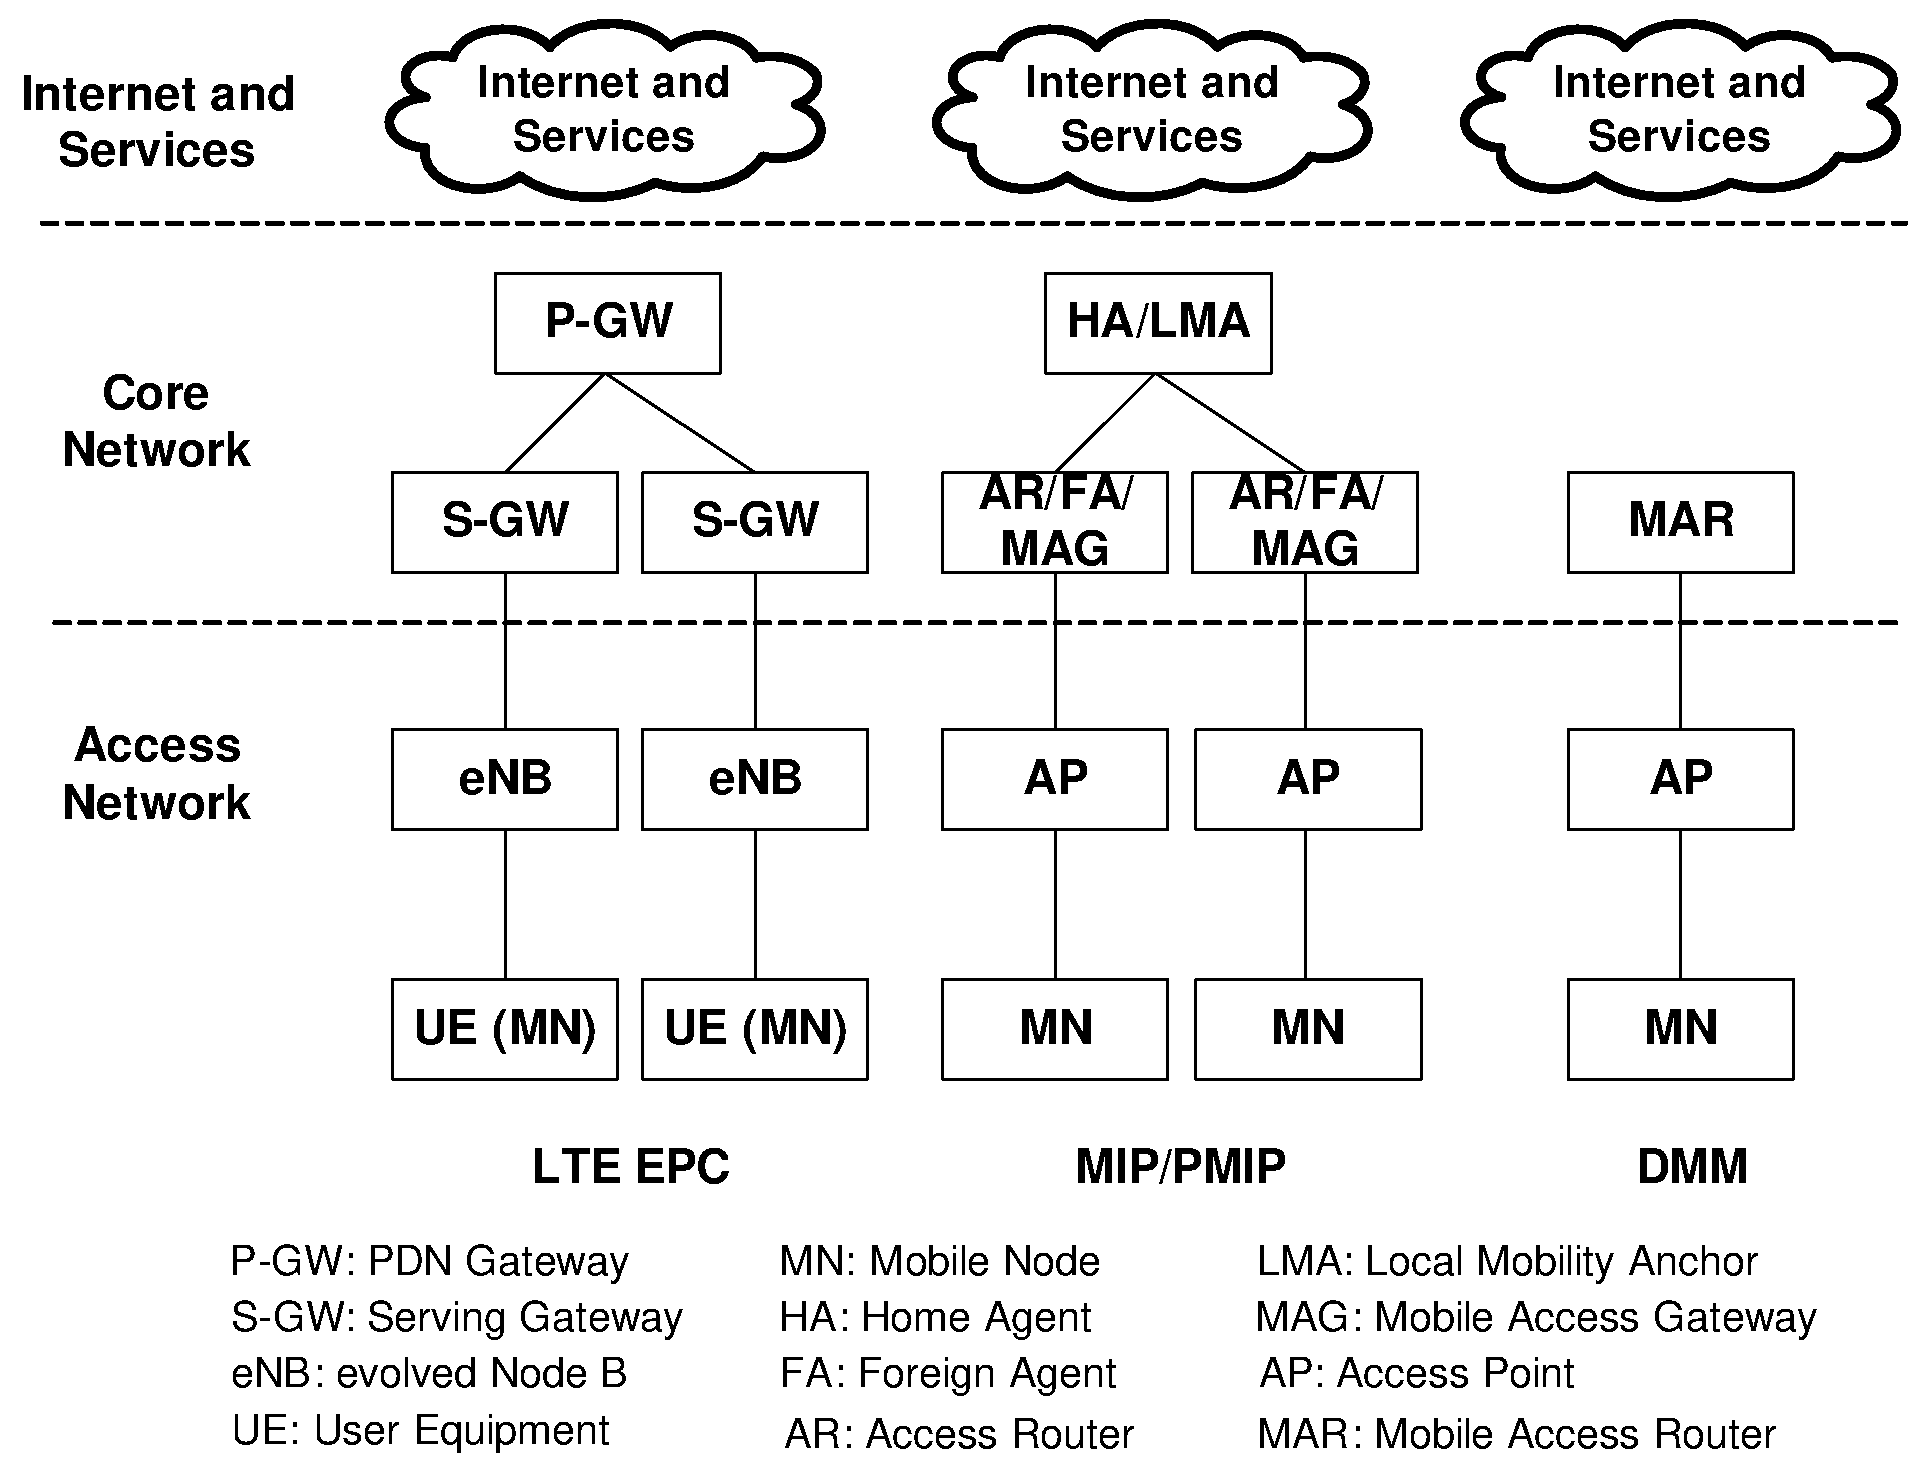
\includegraphics[width=0.70\textwidth]{./Part1/Chapter2/figures/c3_network_level.eps} 
    \caption{Mobile network architecture.}
     \label{fig:c3_network_level}
  \end{center} 
\end{figure}

The current mobile network architecture is highly centralized and hierarchical \cite{DMM_Bertin}. Following the hierarchical architecture, the network elements can be placed into three levels: Internet and services, core network, and access network. For example, the 3GPP cellular network consists of SGSN (Serving GPRS Support Node) and GGSN (Gateway GPRS Support Node). The evolved packet core (EPC) network \cite{3gpp.23.002} includes a packet data network gateway (P-GW), serving gateway (S-GW), and evolved Node B (eNB) as shown in the leftmost of Fig.~\ref{fig:c3_network_level}. Thus IP mobility protocols, such as PMIPv6 and DSMIPv6, which have been adopted as IP mobility protocols for the 3GPP EPC architecture, are inline with the centralized and hierarchical of the network architecture. 

Following the hierarchical architecture, the centralized mobility management protocols rely on the mobility anchor (HA in MIPv6 and LMA in PMIPv6) to enable the mobility support. Therefore, both the mobile context and traffic encapsulation need to be maintained at the mobility anchor. The number of mobile devices and their traffic demand increases exponentially make the centralized mobility management solutions encounter several problems and limitations as stated in \cite{DMM_issues,DMM_problem_statement}. Among them, we just highlight the following issues:

\begin{itemize}
\item \textit{Sub-optimal routing and end-to-end delay}: Since the data traffic always traverses the central mobility anchor, it often results in a longer route, especially when the CN and the MN are close to each other but far from the anchor. The same thing happens in case of Content Delivery Networks (CDN), in which the content providers place their data to the edge of the network. As a result, the end-to-end delay will be increased. 
\item \textit{Scalability problem}: Maintaining MN's context and processing the packets from/to the MN usually require resources of the mobility anchor as well as the networks (require more bandwidth of the links close to the mobility anchor), thus reducing the scalability of the system.  
\item \textit{Resource waste}: The mobility service is always provided even for the sessions that do not require the mobility management support e.g., the sessions which launch and complete while the node is connected to the same layer 3 point of attachment, or the sessions which can handle mobility at the application layer e.g.,  SIP-based sessions. Thus, by providing mobility support for the MN/service when it is really needed, the network resource (e.g., reducing signaling load) can be saved.   
\item \textit{Reliability}: The central mobility anchor in general poses a bottleneck and single point of failure.  
\end{itemize}

\subsection{Distributed Mobility Management}
As stated in the previous section, the mobile network is currently evolving towards the flat architecture. To cope with this evolution, distributed mobility management (DMM) solutions have been proposed. DMM concept aims at addressing the limitations of the centralized mobility approach (e.g., bottleneck and single point of failure, etc.) raised when a large number of mobile devices and data traffic are considered in a flat architecture \cite{DMM_issues,DMM_problem_statement}. DMM is currently a hot topic which gains much interest from both the academia and the industry. The IETF has recently chartered the Distributed Mobility Management (DMM) working group\footnote{IETF DMM WG: https://ietf.org/wg/dmm/charter/} which specifies the solutions allowing for setting up IP networks supporting a distributed anchoring model. The key concepts of DMM are: i) the mobility is distributed among network entities and placed as close as possible to the MN e.g., at the router edge of the access network; and ii) the mobility management is dynamically provided for the sessions that really require service continuity. 

Following the DMM requirement (REQ4) in terms of reusing/extending the existing IETF IP mobility protocols (i.e., MIPv6 and PMIPv6, and so on), the existing proposals (e.g., \cite{DMA, PMIP_based_DMM_Bernardos}) aim at making these solutions work in a distributed manner by deploying multiple mobility anchors (HA in MIPv6 and LMA in PMIPv6) at the edge of the access network, serving as the default gateway of the mobile node. From the IETF point of view, there are two main groups of solutions: the host-based and the network-based. The host-based approach provides a global (as well as a local) mobility support for the MNs while the network-based provides a local mobility support for the MNs moving in a single domain. 
\subsubsection{DMM from IETF Point of View}
\paragraph{Host-based DMM Approach}

The terminology used by this subsection names an access router that provides the host-based DMM mobility support is a Host-based Mobile Access Router (HMAR). The HMAR, similar to HA, is a mobility anchor which allocates a network prefix to the MN and maintains the binding cache for its registered MNs. The current HMAR (cHMAR) is the one to which the MN is currently attached, while the anchor HMAR (aHMAR) of an address/session is the one where the prefix in use is allocated (and the session is initiated using this address as the source address).  

In the host-based approach, the MN is required to participate to the signaling process. There are two main schemes for the host-based approach. In the first scheme, the tunneling for the handover session is established between the anchor HMAR and the MN as similar to the MIPv6 protocol. In the second scheme, the tunnel is established between the current HMAR and the anchor one. 

Regarding the first host-based DMM scheme as proposed in \cite{MIP_based_DMM_Bernardos,MIP_based_DMM_Hassan}, whenever an MN attaches to a HMAR it gets an IPv6 address. The cHMAR plays the role of HA for the address allocated at its network. While attaching to the cHMAR, the MN can start new communications (flows) with the CNs using the current address as the source address of the flows. These new flows are then routed in a standard way without the tunneling mechanism. When the MN performs a handover, if these ongoing flows are still alive, these flows are routed via the routers where the flows were originally initiated (aHMAR) using the tunneling mechanism. Thus, the MN needs to register its current topological location to each aHMAR (corresponding to each active HoA in use) by means of BU/BA messages. In this case, the current HoA actually plays the role of CoA. A bi-directional tunnel is then established between each aHMAR and the MN. Thus, the traffic passes through the mobility anchor via the bi-directional tunnel. Fig.~\ref{fig:c3_mip_dmm} and Fig.~\ref{fig:c3_mip_dmm_signaling} represent an example scenario of host-based DMM support.

It is noted that the MN should perform a location update process for each active IP address. As a result, it requires the MN to manage the list of active HoAs and the associated aHMARs, as well as the list of active sessions using the corresponding HoA. Moreover, the MN needs an additional mechanism which allows to select the right IP address to use for each session. The binding cache of the HMARs and the list of active sessions of the MN are illustrated in Fig.\ref{fig:c3_mip_dmm_b}.
\begin{figure}[h!]
\centering
\subfloat[]{\includegraphics[width=0.47\textwidth]{./Part1/Chapter2/figures/c3_mip_dmm.eps} \label{fig:c3_mip_dmm_a}}\,\,\,\,\,\,
\subfloat[]{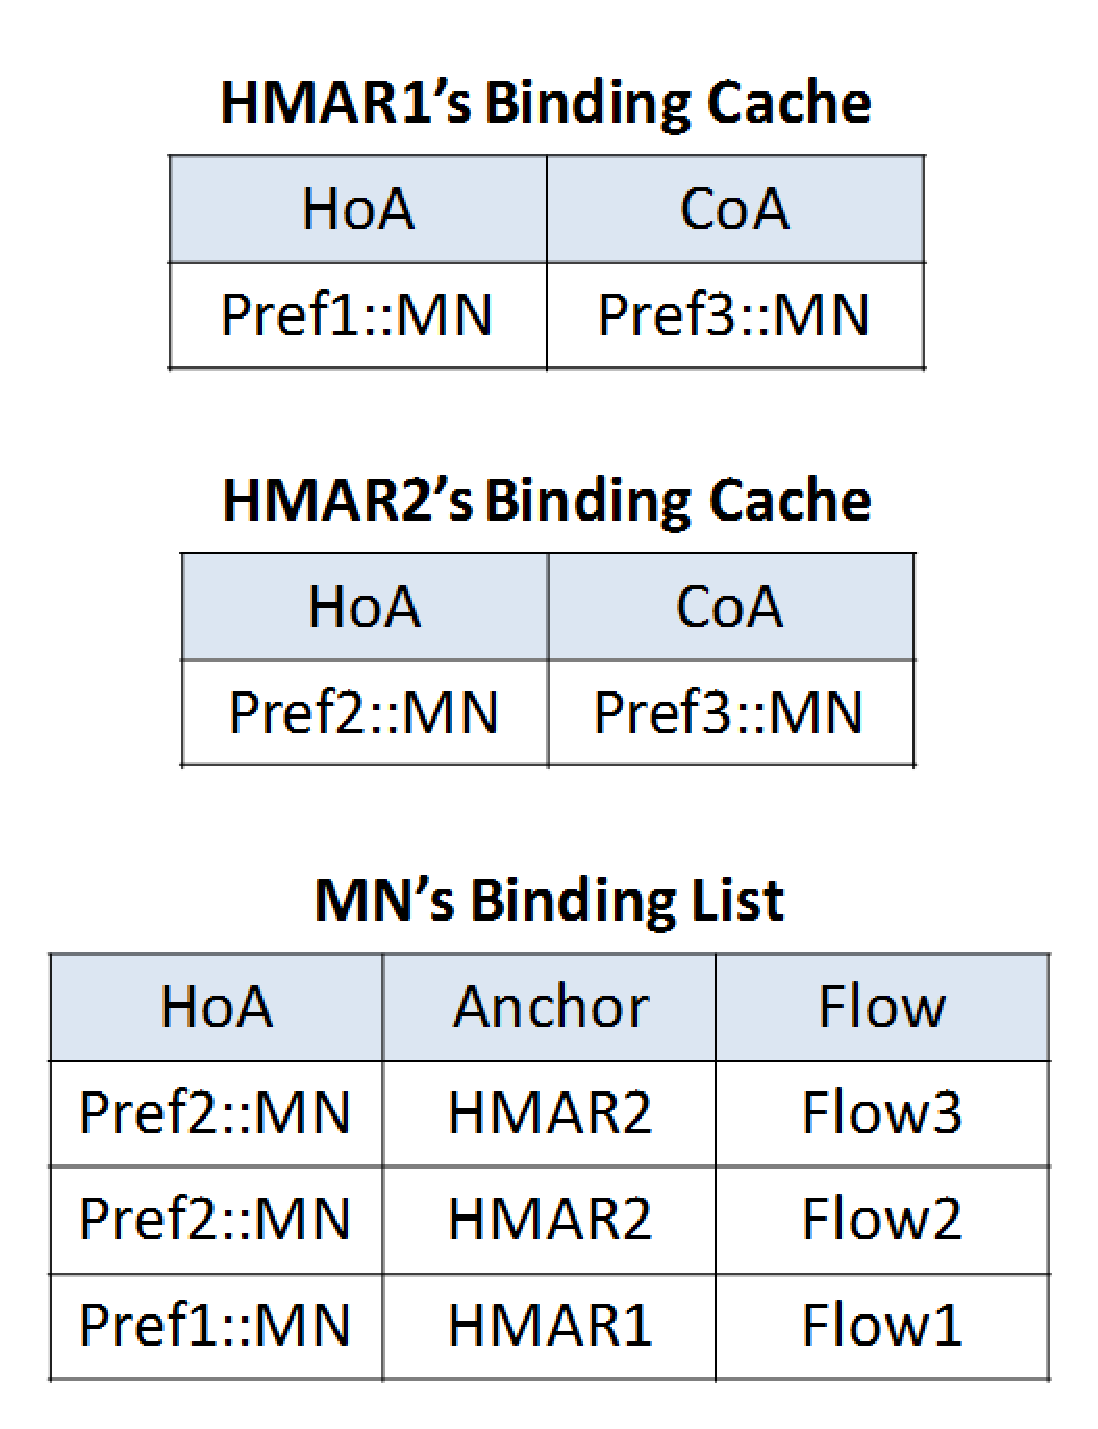
\includegraphics[width=0.33\textwidth]{./Part1/Chapter2/figures/c3_mip_dmm_b.eps}\label{fig:c3_mip_dmm_b}}
\caption[Mobility management in the host-based approach (scheme 1).]{Mobility management in the host-based approach (scheme 1): (a) Operation description. (b) Binding cache.}
\label{fig:c3_mip_dmm}
\end{figure}
\begin{figure}[h!] 
 \begin{center} 
 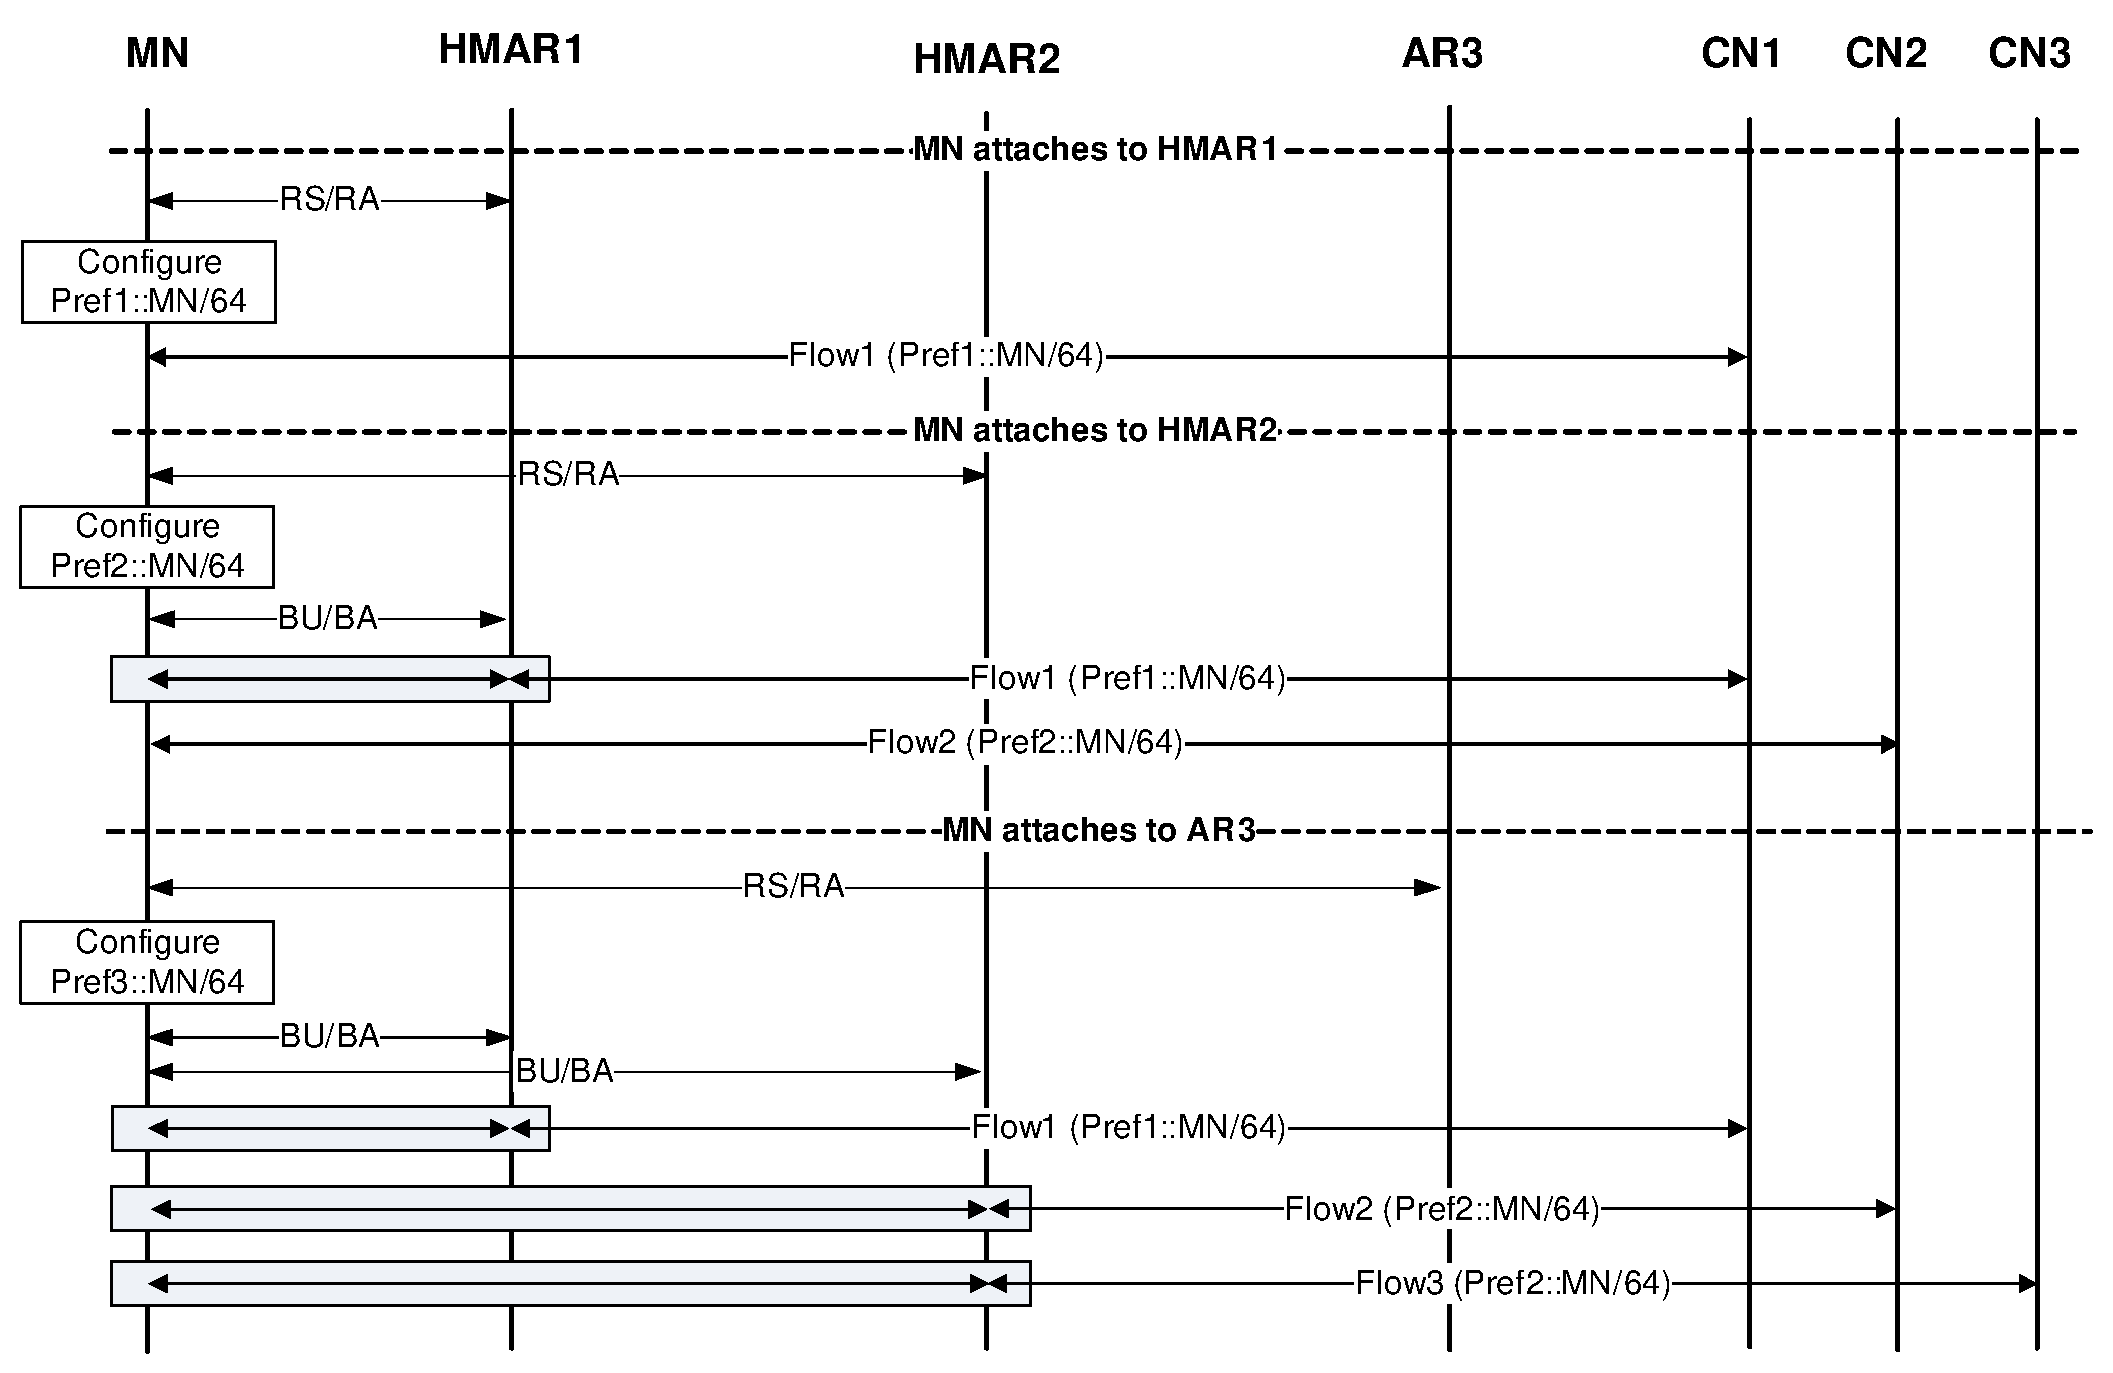
\includegraphics[width=0.9\textwidth]{./Part1/Chapter2/figures/c3_mip_dmm_signaling.eps} 
    \caption{Signaling for the mobility management in the host-based approach (scheme 1).}
     \label{fig:c3_mip_dmm_signaling}
  \end{center} 
\end{figure}

Additionally, as a global mobility, another scenario should be taken into account in which the MN moves to a typical access router's area (without supporting the host-based DMM) as discussed in \cite{DMM_analysis_Hassan, MIP_based_DMM_Condeixa}. In this circumstance, the MN should select one among the active IP addresses to be served as the source address, and the associated aHMAR as the HA. The MN then performs the normal MIPv6 operation. For example, as shown in Fig.\ref{fig:c3_mip_dmm}, the MN attaches to a typical access router (AR3). After getting a prefix (Prefix3::/64), the MN configures its IP address (Pref3::MN/64). When the MN starts a new session (Flow3), it selects HoA2 and HMAR2 as the source address and the corresponding HA, respectively. As a result, the Flow3 is routed via the tunnel HMAR2-MN. Regarding the ongoing flows, the Flow1 and Flow2 are then routed via HMAR1 and HMAR2 using the tunnel HMAR1-MN and HMAR2-MN, respectively.

As stated earlier, the MN needs to inform all active aHMARs about its current location by means of BU/BA messages. Thus, the mobility signaling cost (over the air) is relatively high. As a result, the second host-based DMM scheme is proposed in order to reduce the mobility signaling cost of the MN (see Fig.\ref{fig:c3_mip_dmm_2}). In this case, the MN only needs to exchange the BU/BA messages with the current mobility anchor \cite{DMM_IETF_Lee}. The BU includes the MN's prefixes in use and the corresponding aHMAR. Based on this information, the BU/BA messages are exchanged between the cHMAR and each aHMAR which allows establishing the tunnel between them. The active sessions are then routed via the corresponding aHMAR utilizing the tunneling mechanism. Again, if the MN moves to a typical AR's area, the tunnel is established between the MN and the aHMAR as similar to the previous host-based scheme.  
\begin{figure}[h!]
\centering
\subfloat[]{\includegraphics[width=0.47\textwidth]{./Part1/Chapter2/figures/c3_mip_dmm_2.eps} \label{fig:c3_mip_dmm_2_a}}\,\,\,\,\,\,
\subfloat[]{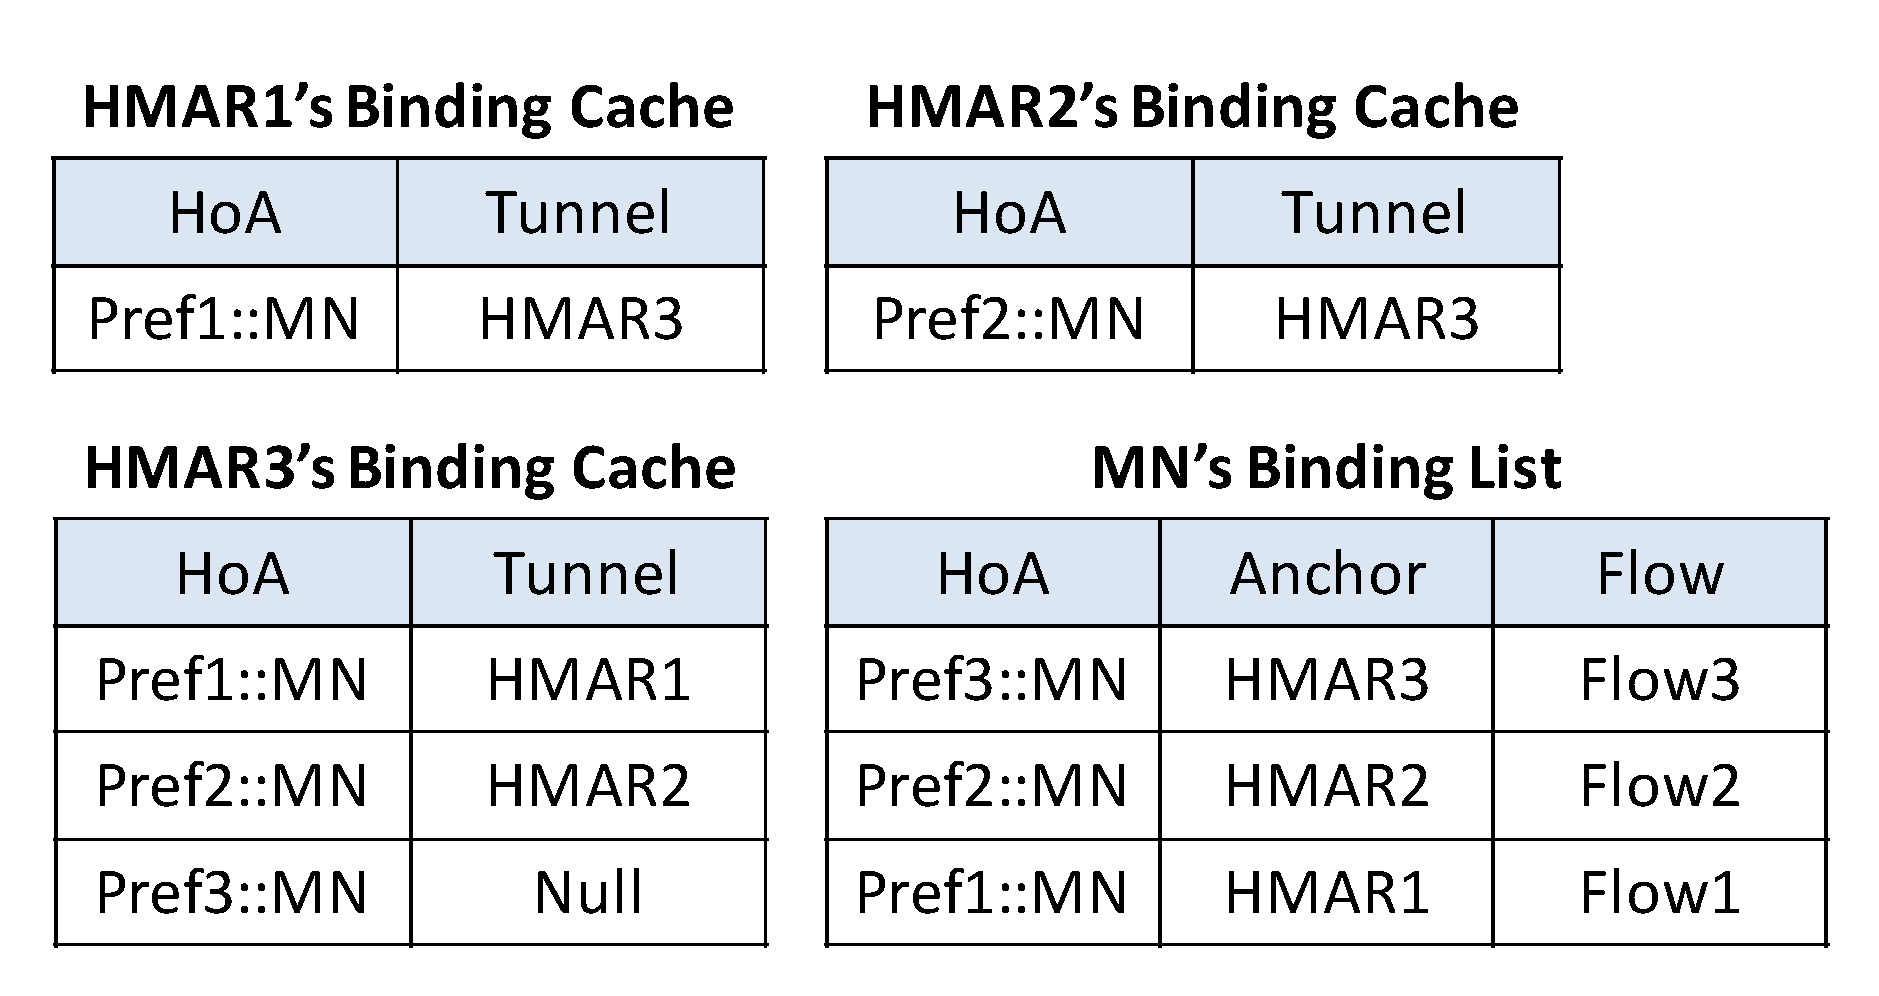
\includegraphics[width=0.47\textwidth]{./Part1/Chapter2/figures/c3_mip_dmm_2_b.eps}\label{fig:c3_mip_dmm_2_b}}
\caption[Mobility management in the host-based approach (scheme 2).]{Mobility management in the host-based approach (scheme 2): (a) Operation description. (b) Binding cache.}
\label{fig:c3_mip_dmm_2}
\end{figure}

It is important to note that the MN keeps the information of the active HoAs and their associated aHMAR when having at least one active session using this HoA. Otherwise, the information will be deleted. Thus, in this thesis, we suggest that at least one HoA should be considered as a global address and should be kept throughout its lifetime e.g., an address allocated at the MN's typical location. 

\paragraph{Network-based DMM approach}
Unlike the host-based DMM, the network-based approach does not require the MN to participate in the mobility signaling process. To do so, a new network entity, namely Network-based DMM Access Router (NMAR) is introduced. The NMAR is an access router supporting the network-based DMM mobility. The NMAR thus performs both LMA's and MAG's functionality. Acting as a MAG, the NMAR detects the attachment of the MN, while as an LMA it allocates a HNP to the MN. Again, we introduce two logical NMARs: i) a current NMAR (cNMAR) is the NMAR to which the MN is currently attached; and ii) an anchor NMAR (aNMAR) is the NMAR to which the MN's HNP is allocated (the session is initiated). 

Similar to the host-based DMM, when an MN attaches to a NMAR, it obtains an IPv6 address. Typically, it uses the current IP address to start new sessions. The data traffic is routed using the normal IP routing without any tunneling mechanism. If the MN performs a handover and some sessions are still alive (namely handover sessions), the mobility management procedure is activated as follows. The cNMAR, acting as the MAG, exchanges PBU/PBA messages with the aNMAR which acts as the LMA of the flows initiated at the aNMAR. Once the PBU/PBA signaling is completed, a tunnel is established between the cNMAR and the aNMAR for the sessions initiated at the aNMAR. However, an important question raised is that how the nNMAR learn about the addresses of the aNMARs. 
\begin{figure}[h!]
\centering
\subfloat[]{\includegraphics[width=0.50\textwidth]{./Part1/Chapter2/figures/c3_pmip_dmm.eps} \label{fig:c3_pmip_dmm_a}}\,\,\,\,\,\,
\subfloat[]{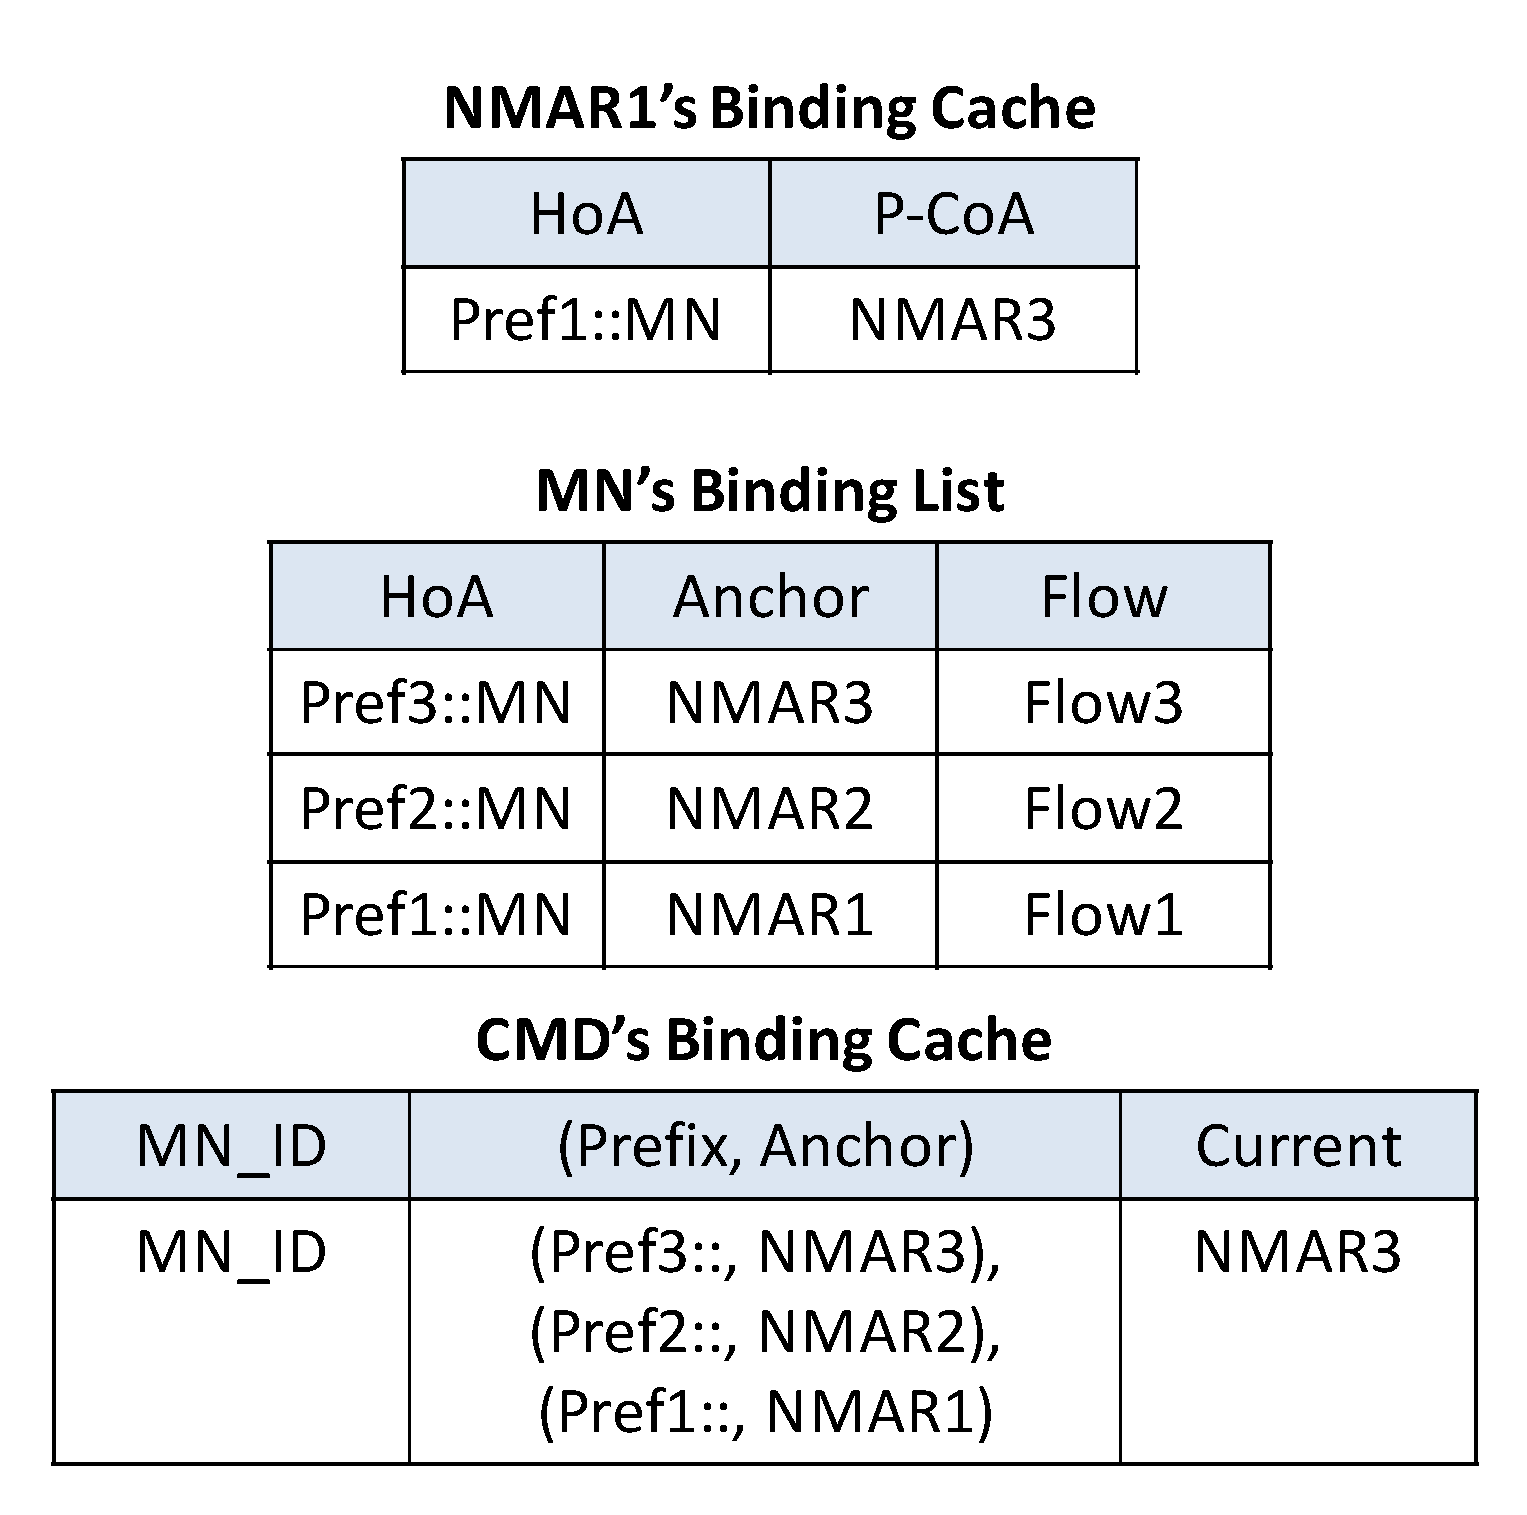
\includegraphics[width=0.39\textwidth]{./Part1/Chapter2/figures/c3_pmip_dmm_b.eps}\label{fig:c3_pmip_dmm_b}}
\caption[Mobility management in the network-based approach.]{Mobility management in the PMIP-based approach: (a) Operation description. (b) Binding cache.}
\label{fig:c3_pmip_dmm}
\end{figure}

There is several mechanisms allowing the nNMAR to know the address of the aNMARs. The first method \cite{DMA} relies on a centralized database (namely centralized mobility database, or CMD) which stores the mobility-related information of each MN in the domain such as the list of MN's HoAs, the associated aNMARs' address as similar to in \cite{inter_domain_DMM}. Although it ensures that the mobility process is totally transparent to the MN, this mechanism introduces again a centralized anchor, however, for control plane only. The data plane is still fully distributed among the network entities. That is the reason why this scheme is considered as a partially distributed scheme. The second method relies on the information provided by the MN as specified in \cite{PMIP_based_DMM_Giust}. In other words, the NMAR retrieves the address of the anchor NMARs from the MN. As a result, the MN is no longer transparent to the mobility process. Therefore, in some papers \cite{DMM_analysis_Hassan, DMM_IETF_Lee} this method is considered as a host-based scheme as stated above. 
\begin{figure}[h!] 
 \begin{center} 
 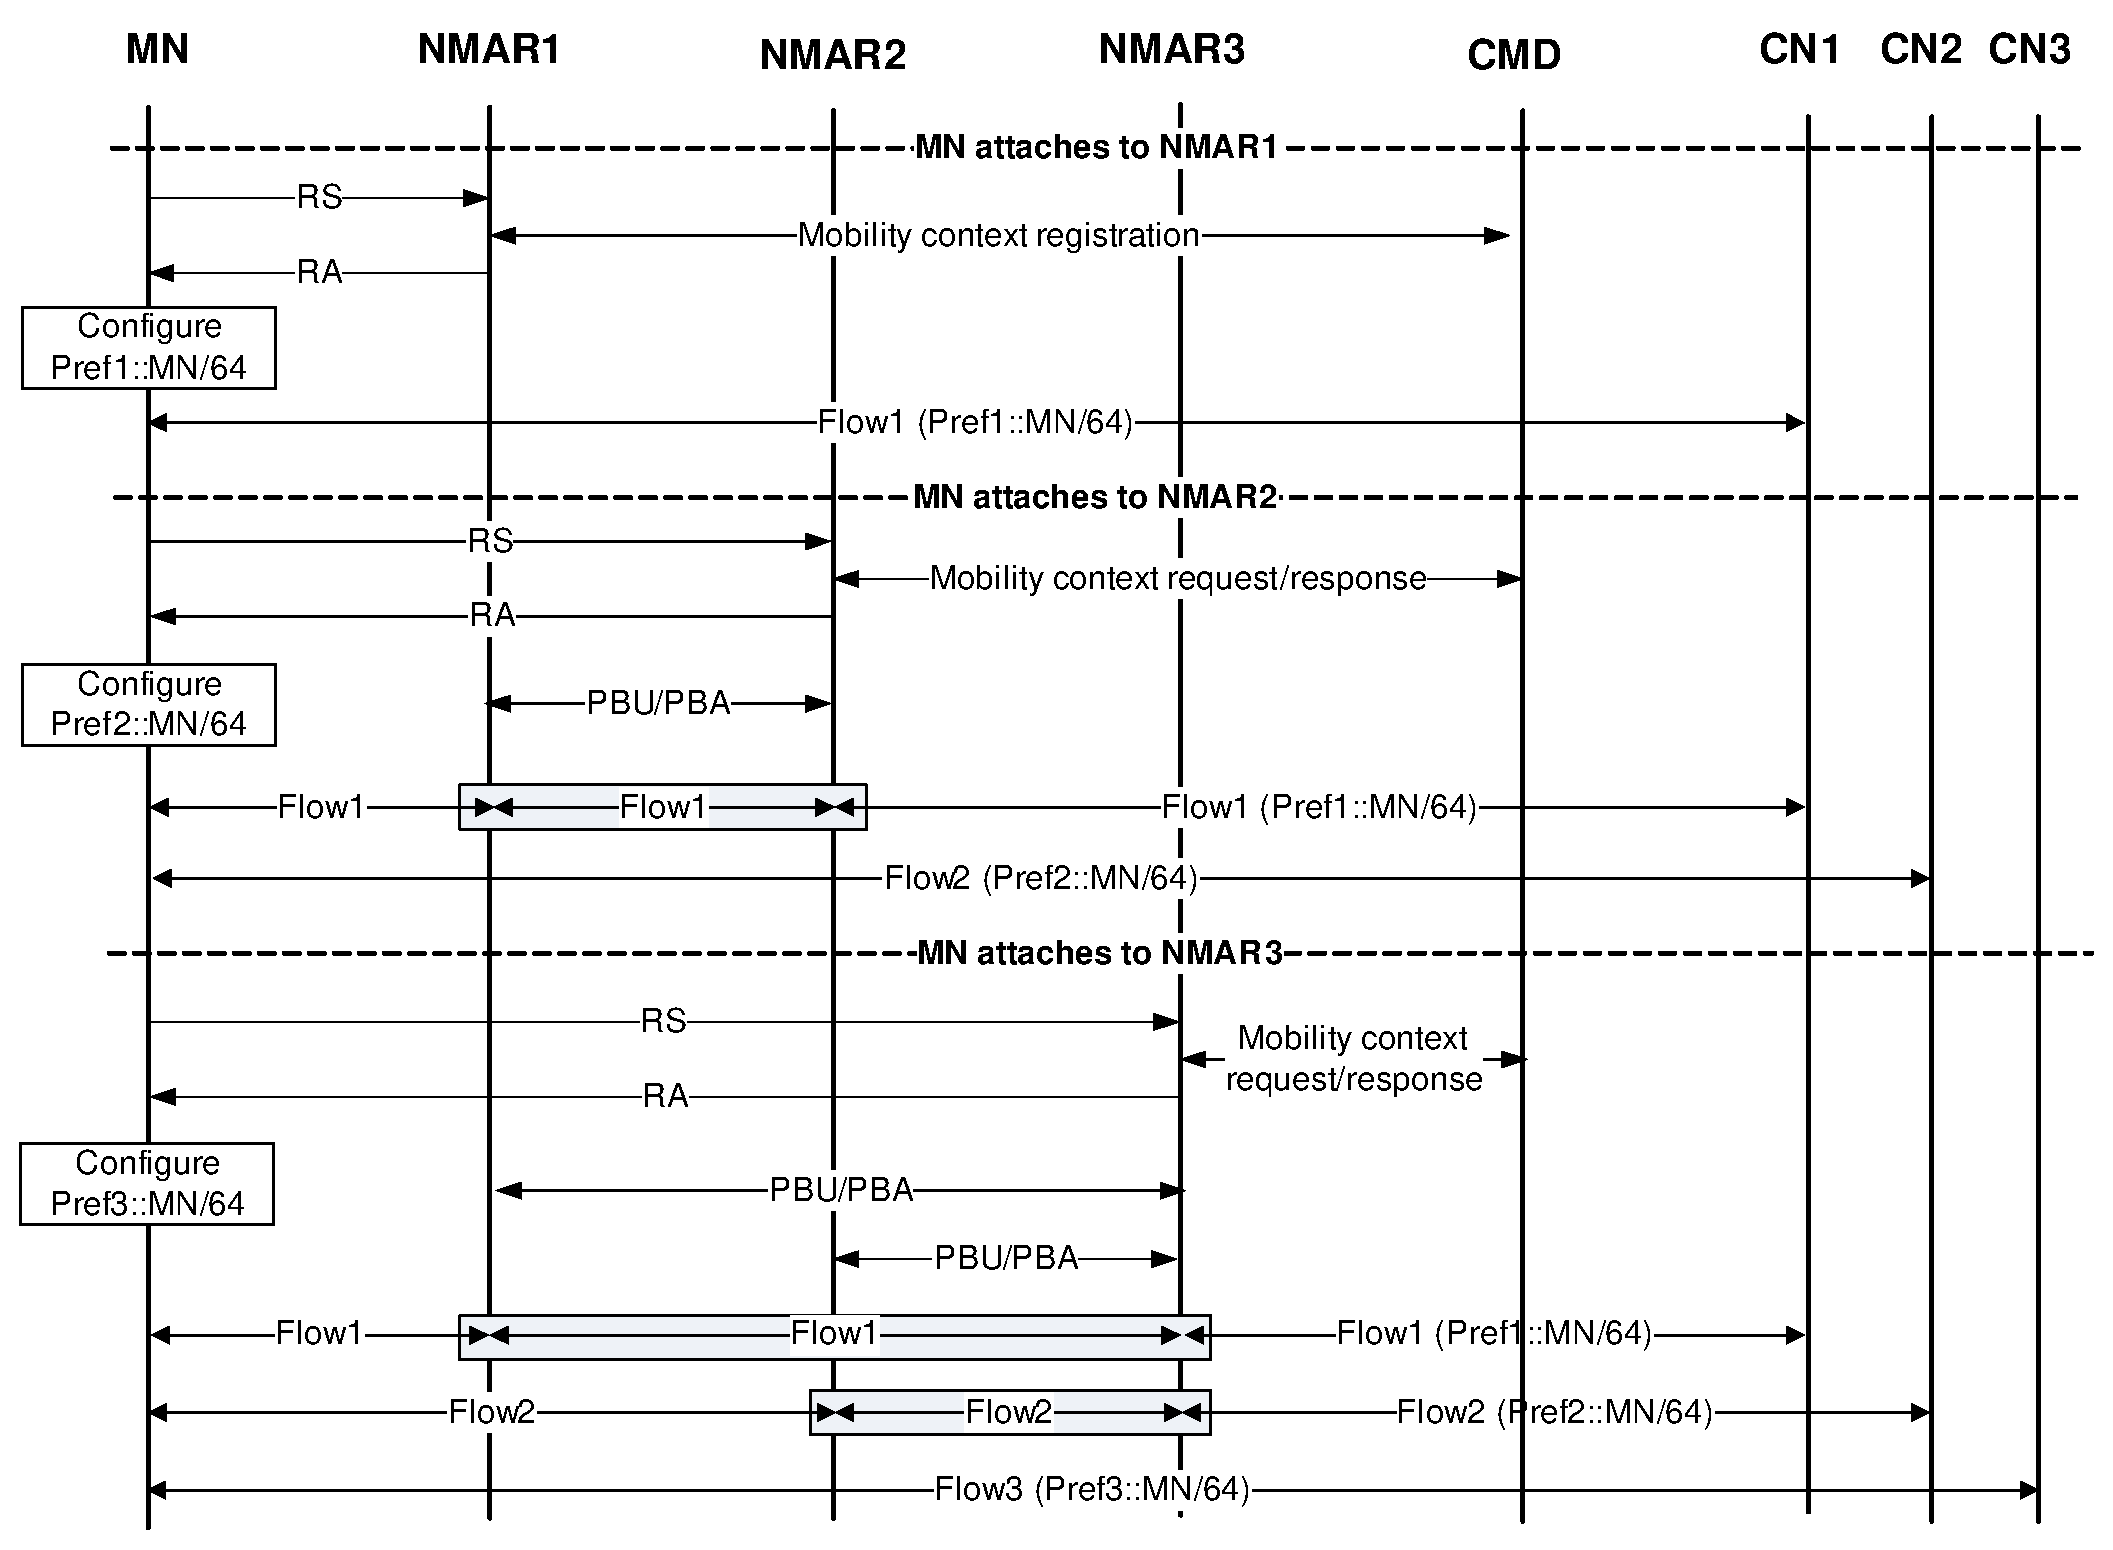
\includegraphics[width=0.9\textwidth]{./Part1/Chapter2/figures/c3_pmip_dmm_signaling.eps} 
    \caption{Signaling for the mobility management in the network-based approach.}
     \label{fig:c3_pmip_dmm_signaling}
  \end{center} 
\end{figure}

 The diagram in Fig.~\ref{fig:c3_pmip_dmm_signaling} depicts the operations of the partially distributed DMM. When an MN attaches to the network-based DMM domain (for example at NMAR1), after detecting the presence of a new MN by means of receiving a RS message (including the MN's ID), the NMAR1 allocates a HNP (Pref1::/64) for the MN. It then sends a mobility context request (MC-Req) message including the MN\_ID and the Pref1::/64 to the CMD to register the new prefix and retrieve the existing mobility context of the MN (if exist). The CMD then checks its mobility database for this MN. Since it is the first time the MN is attached to this domain, there is no entry for it. Therefore, the CMD creates an entry (for the MN) including the MN\_ID, Pref1::/64 and the associated NMAR (NMAR1). The CMD sends a mobility context response (MC-Res) message indicating that the information of the MN is successfully registered. Afterwards, the NMAR1 sends a RA including the allocated prefix (Pref1::/64) to the MN. Based on this information, the MN configures its IPv6 address (Pref1::MN/64) and starts a new communication with the CN1 (Flow1), following the normal way. As the MN moves to the access network of NMAR2,  the NMAR2 allocates a new HNP (let say Pref2::/64) for the MN. It then sends a MC-Req message to the CMD for the new prefix registration and for retrieving the existing mobility context of the MN. Upon receiving the MC-Req message and searching its mobility context table, the CMD updates the MN's mobility entry corresponding to the new prefix (as in Fig.~\ref{fig:c3_pmip_dmm}). The CMD then replies by a MC-Res message including the MN\_ID and the list of its active prefixes, and the associated NMARs (in this case is Pref1::/64 and NMAR1). Upon the reception of the MC-Res message, the NMAR2 updates its BCE and routing for Pref2 and sends a RA to the MN which includes the Pref2::/64. The PBU/PBA messages are then exchanged between the NMAR2 and the NMAR1 to sets up the bi-directional tunnel between them for the Flow1. Regarding the MN, after receiving a RA, it configures its IP address (Pref2::MN) and uses it to start a new communication with the CN2 (Flow2) in a normal way. The similar thing happens when the MN moves to NMAR3. In this case, the Flow1 and Flow2 are routed through the NMAR1 and NMAR2, respectively. In the mean time, the Flow3 which is initiated when the MN attaches to NMAR3, is routed in a normal way without the tunneling mechanism. 

Besides, there are proposals which apply the DMM concepts into the PMIPv6 domain. For example, in \cite{PMIP_based_DMM_Korhonen}, the locally assigned prefixes mechanism within a PMIPv6 domain is proposed. In this case, the MAG can attribute its own prefix (the so-called local prefix) to the MN which can be used for the communication by passing the LMA when the MN is currently attached to the MAG. The MN can still use the IP address allocated by the LMA in a typical PMIPv6 way.  
\subsubsection{DMM Consideration in 3GPP}
\begin{figure}[h!]
\centering
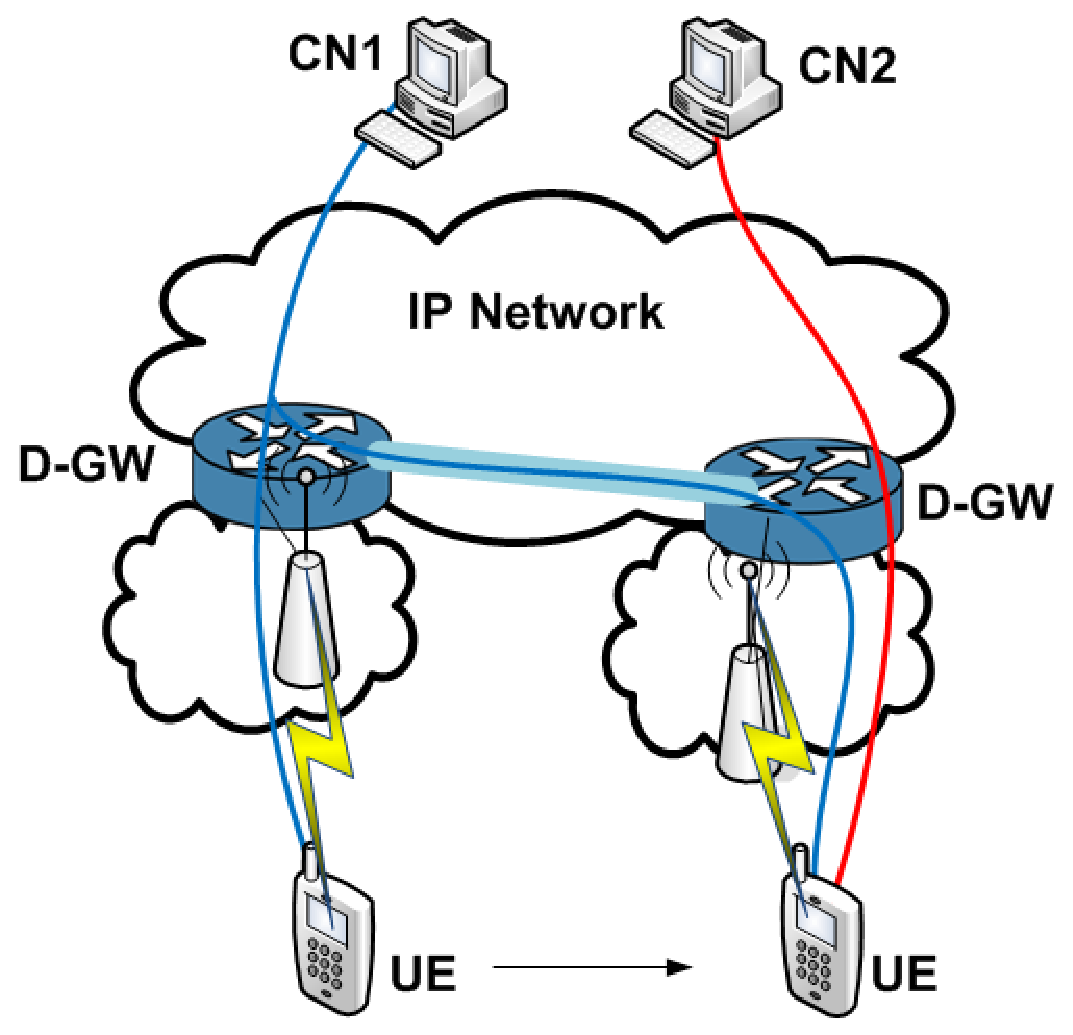
\includegraphics[width=0.38\textwidth]{./Part1/Chapter2/figures/c3_dmm_3gpp.eps}
\caption[Mobility management for 3GPP.]{Mobility management for 3GPP}
\label{fig:c3_dmm_3gpp}
\end{figure}

In order to deal with a huge number of traffic demands as well as the revenue per data decreasing phenomenon, 3GPP proposes such traffic offload mechanisms as SIPTO, LIPA and IP Flow Mobility (IFOM). The main idea is that the user data can be routed bypassing the core network based on certain conditions. In more details, SIPTO supports offload of certain types of traffic directly to the Internet and away from the mobile core network. It is done by selecting a set of S-GWs and P-GWs that are geographically/topologically close to the User Equipment's point of attachment (UE is an MN following the 3GPP terminology). However, the offloaded traffic cannot access the operator services. On the other hand, LIPA enables a UE connected via a Home eNB (HeNB) to access the IP capable entities in the same residential/enterprise IP network without the data traversing the mobile operator’s core. Although, SIPTO/LIPA is similar to DMM in terms of traffic offloading (mitigating the traffic aggregation at the core network), there is a limited mobility support. For example, LIPA supports only the mobility between HeNBs managed by the same Local-GW (L-GW) while SIPTO enables mobility support for the case S-GW/P-GW is at/above Radio Access Network (RAN). In other words, 3GPP has not yet considered the mobility of UE, which may result in service disruption when a UE is on the move. In fact, SIPTO/LIPA can be considered as a step towards DMM from conventional centralized/hierarchical approaches. It comes from the fact that based on SIPTO/LIPA the functionality of P-GW is distributed by deploying multiple L-GWs. In the next step, by re-using the existing S5 interface (PMIPv6 tunneling), the mobility between the L-GWs can be enabled. From that point, it is feasible to support DMM in LTE/SAE by simply installing the DMM functionality at the distributed L-GWs (called Distributed Gateway or D-GW) as illustrated in Fig.~\ref{fig:c3_dmm_3gpp}. 

\subsection{Other Considerations}
\subsubsection{Mobility across Heterogeneous Networks}
With the evolution of mobile communication systems (wireless technology and network architecture), heterogeneous networks provide the possibility to greatly increasing capacity at a low cost. In this context, the seamless mobility across different types of wireless access technology e.g., WLAN, WiMAX and LTE needs to be taken into account. Regarding the network infrastructure, IEEE 802.21 Media Independent Handover (MIH) services allow optimizing the handovers between heterogeneous IEEE 802 and cellular networks. The handover performance can be enhanced using the layer-2 information available from IEEE 802.21 services. From the mobile node point of view, to maintain the session continuity, additional techniques (as specified in \cite{PMIP_EV}) should be considered which allow the MN to obtain the same IPv6 address after handover across different access technologies. Among them, the logical interface technique \cite{logical_interface} can help to hide the different access technologies, thus, the changing of interface is transparent to the IP stack. Moreover, the interfaces of the MN can be active at the same time, which helps reducing the handover latency. 

\subsubsection{Network Mobility}
Network Mobility (NEMO)\footnote{NEMO IETF WG: http://datatracker.ietf.org/wg/nemo/} refers to the mobility of an entire network which changes its point of attachment to the Internet. Thus, the main purpose of NEMO support is that it allows every node in the mobile network to be reachable while moving around. Moreover, the mobility should be transparent to the nodes insides the mobile network. The basic network mobility support is based on MIPv6 to enable the network mobility in an IPv6 network. 

In order to provide the mobility support for a Mobile Network, a specific gateway called Mobile Router (MOR) is introduced. The MOR will be connected to the fixed infrastructure and provides connectivity to the nodes inside the Mobile Network. Like the mobility support of a mobile node (host-based approach), the NEMO basic support (as specified in \cite{NEMO}) is also based on the bi-directional tunnel between the MOR and its HA to enable mobility support when the MOR is away from home. Thus, as a topological anchor point of MOR's address, the data packets addressed to the mobile network are delivered to the HA, which then tunnel them towards the MOR. The MOR, after removing the tunnel headers, forwards the data packets to the destination inside the mobile network. Note that similar to normal MIPv6 operation where the binding association between the HoA and the CoA is maintained in the Binding Cache, in NEMO, the HA might also keep the Mobile Network Prefixes (MNP) in the corresponding BCE. As a result, in a large-scale development, the MNP allocation should be considered as in \cite{NEMO_DHCP}. 
 
\subsubsection{Comparison between the Mobility Management Approaches}
As stated earlier, the performance of a mobility management protocol is typically measured using such metrics as signaling cost, handover latency, and packet loss. Based on these metrics, various papers have been presented to evaluate the performance of the mobility management protocols. 

Comparative performance analysis for the host-based mobility management protocols e.g., MIPv6, FMIPv6, HMIPv6 and F-HMIPv6 in terms of signaling cost, handover latency, and packet loss has been carried out in \cite{HO_comparison_Montavont, HO_comparison_Makaya,HO_comparison_Costa}. In \cite{HO_comparison_Lee,HO_comparison_Lee_2,HO_comparison_Lee_3}, the authors also took into account the network-based mobility management protocols e.g., PMIPv6 and FPMIPv6 in the comparative performance analysis. From these analysis, some conclusions are: i) Using layer 2 information generally helps to reduce the handover latency and packet loss at a cost of signaling overhead. However, it depends on each link-layer technology; ii) The network-based mobility management protocols reduce the signaling overhead over the air of the MN compared to the host-based mobility protocols; and iii) Typically, the handover latency and the signaling cost depend on the network topology in use. In other words, the hop distance between the network entities is an important factor influencing the performance of these protocols.  

Regarding DMM, a lot of research publications \cite{DMM_Bertin, PMIP_based_DMM_Giust, DMM_IETF_Lee, MIP_based_DMM_Condeixa, MIP_based_DMM_Hassan, DMM_analysis_Hassan} have carried out the analysis on different DMM approaches, compared them with the conventional mobility managements in terms of signaling cost, packet delivery cost, handover delay, packet loss and end-to-end delay. The results from these analysis showed that DMM is a promising mobility management scheme. In details, in \cite{DMM_Bertin} the authors conducted a simulation to compare DMM and MIPv6 (with handover optimizations). The simulation results showed that DMM outperforms MIPv6 in terms of handover delay and TCP delay. In \cite{DMM_IETF_Lee}, both qualitative and quantitative comparison for centralized mobility management protocols and DMM protocols are provided. Also, the comparison in terms of handover latency, signaling cost and data delivery cost has been conducted in \cite{MIP_based_DMM_Condeixa}. 

\section{IP Mobile Multicast}
The increasing penetration of the mobile devices, such as tablets and smart phones is generating a huge number of data traffic over mobile networks. The majority of this traffic is video data: estimates say that mobile video traffic will account for 66.5\% of total mobile data traffic by 2017 \cite{cisco_forecast}. In this context, the scalability and the bandwidth efficiency from the multicast routing make the IP multicast a remarkable solution from application point of view to allow mobile networks to deal with a huge number of traffic, particularly in mobile environments where users usually share frequency bands and limited capacity \cite{Multicast_MIPv6}. In other words, when a large group of users is simultaneously interested in the same content, the multicast can provide significant advantages compared to the unicast in terms of resources efficiency both from the perspectives of the network and of the servers \cite{developing_ip_multicast}. However, one of the major challenges for multicast support is when mobility is considered.

About the IP mobile multicast, after more than a decade of research and development efforts, many approaches have been proposed, but most of them are based on such host-based mobility management protocols as MIPv6, FMIPv6 and HMIPv6. However, the main drawback of these host-based mobility management protocols is that they require the MN to modify its IP stack to participate into the mobility signaling process. As a result, the previous IP multicast approaches introduced in \cite{Multicast_MIPv6, multicast_challenges_solutions} cannot be directly applied in a network-based mobility management in which the MN is unaware of the mobility process.

Recently, a base development of multicast listener support in PMIPv6 has been adopted by the IETF. However, it does not provide any specific optimization and performance enhancements such as service disruption and packet loss, sub-optimal routing, and packet duplication. Several solutions have been proposed in order to address couple of issues. In this section, we give a brief overview to the multicast mobility-related problems and enlist some possible solutions in MIPv6 to highlight the main idea of these proposals. Based on that, we then take a deep analysis on the multicast mobility in a PMIPv6 and a DMM environment. 

\subsection{Overview of Multicast Mobility in Mobile IP}
In order to enable multicast in Mobile IP (both Mobile IPv4 and Mobile IPv6), two basic approaches have been proposed i.e., bidirectional tunneling and remote subscription. Both approaches have their own advantages and drawbacks. The bidirectional tunneling hides the movement of the multicast nodes by tunneling the multicast traffic via the mobility tunnel between the node and its HA at the cost of triangular routing (leading to a long delay) and tunnel convergence problem. On the other hand, in the remote subscription approach, the multicast node has to rejoin the on-going multicast sessions after each handover, leading to the potential significant service disruption. In addition, more serious problems can be raised in case of source mobility such as address transparency and routing state maintenance \cite{Multicast_MIPv6, multicast_challenges_solutions}. Further enhancement should also be considered in order to meet the additional requirements in terms of service disruption and packet loss for the real-time services. Therefore, various methods have been proposed to improve the two essential solutions. In \cite{multicast_challenges_solutions,Multicast_MIPv6}, the authors provides a survey of numerous proposals for the multicast listener as well as the source mobility. 

From listener point of view, several solutions \cite{MoM, RBMoM,MPDSR, MMA} have been proposed to construct an efficient multicast delivery tree. In more details, the Mobile Multicast Protocol (MoM) \cite{MoM} aims at solving the tunnel convergence problem by selecting one HA which serves as a common HA (per group) for all listeners subscribed to a multicast group at the same visited network. In other words, a single tunnel between the selected HA and the FA is used for multicast delivery between the home network and the foreign network. The Range-Based Mobile Multicast (RBMoM) \cite{RBMoM} trades off the shortest delivery path and the frequency of multicast delivery reconstruction, however, it introduces much of complexity. The Multicast Protocol With Dynamic Service Range (MPDSR) \cite{MPDSR} enhances RBMoM to reduce the number of multicast tree reconstructions and multicast service disruption time. In general, MoM, RBMoM and MPDSR can be considered as an enhancement of the bidirectional tunneling approach. The Multicast By Multicast Agent Protocol (MMAP) \cite{MMA}, as an enhancement of the remote subscription approach, uses the tunnel between the previous foreign network and the current one for delivering the multicast traffic to reduce the tunnel convergence problem and the service disruption. In \cite{multicast_ip_Jelger}, the authors proposes combining the bidirectional tunneling and the remote subscription. They also discusses the practical aspects of the bidirectional tunneling approach. Besides, \cite{seamless_multicast_MIPv6, FPMIPv6_multicast,fast_multicast_Kwon} mainly aim at addressing the problem of packet loss and multicast service disruption by extending the fast handover protocols for multicast support.  

From multicast source point of view, the bidirectional tunneling approach preserves the transparency of the movement of the source. However, it suffers the triangular routing, long service latency, and inefficient in packet delivery which impact the overall listeners. The remote subscription approach helps to address these issues, yet, the movement of the source causes the address transparency and tree reconstruction. Thus, the multicast routes should be updated to reflect the current location of the source in an appropriate manner to effectively avoid the packet loss. There are two main types of solution in which the traffic will be injected to the old tree or the overall delivery tree will be reconstructed \cite{Multicast_MIPv6}. The additional complexity is raised in case of SSM. For example, in \cite{tree_morphing_Schmidt, tree_morphing_Christ}, the authors propose a tree morphing protocol to address the address transparent issue allowing a continuous adaptation of multicast shortest path trees to the source mobility. However, the complexity and high signaling cost could be added, as all the MRs need to be extended. Similarly, in \cite{PMIP_multicast_source_Lee}, the authors propose a state update mechanism by reusing the legacy multicast tree for a minimization of packet delay. In \cite{host_identity_multicast}, the authors, based on the Host Identity Protocol, introduce multicast routing states which is independent of IP addresses. Further approaches can be found in \cite{multicast_challenges_solutions,Multicast_MIPv6,multicast_source_Wang}. 

Since all these mobile multicast protocols are designed for MIPv4 and MIPv6 which require the mobile nodes to participate in the signaling process, they cannot be directly applied to PMIPv6. Yet, the idea of these solutions can be re-used. 

\subsection{Multicast Mobility in PMIPv6}
As the multicast protocols (group management and routing protocols) are originally designed for a fixed network, considering multicast in a mobile environment brings several challenges to the multicast service. The mobility of the node  (e.g., the change of point of attachment and of globally reachable IP address) has different impacts on the multicast service, depending on such factors as the role of the node in the multicast session (source or listener), the considered multicast model (ASM or SSM), the multicast routing protocol, the multicast group management protocol and the mobility protocol in use as well as the wireless access technology. Therefore, the IP mobile multicast issues can be divided into four main groups: the general multicast problems (due to multicast protocols), the specific mobile listener problems, the specific mobile source problems and the deployment issues \cite{Multicast_MIPv6, multicast_challenges_solutions,tuning_MLD}.

\subsubsection{Multicast Mobility Issues}
Prior to taking more details on the multicast mobility issues, we will look at some requirements of the multicast support in PMIPv6. First, the session continuity should be provided when a listener/source moves from one IPv6 subnet to another. In addition, the noticeable service disruption and the significant packet loss should be avoided during handovers. Especially, in the context of a network-based mobility management protocol, the mobile node should remain unaware of mobility from the network layer and the application point of view. Then, it is desirable to preserve the characteristics of multicast such as effectiveness of delivery (to avoid traffic duplication and tunneling overhead) and approximate optimal routing. 

\paragraph{General Issues}
At the beginning, the multicast protocols are designed for a fixed environment using wired connection. Thus, considering these protocols in a mobile and wireless environment can raise several challenges. Particularly, considering the multicast group management protocols (IGMPv3 and MLDv2), which typically work in the wireless access network (MN and first hop AR), may lead to such issues as the multicast-related signaling overhead, the multicast service disruption and the long leaving latency \cite{tuning_MLD}. Additionally, wireless is typically an unreliable media, that means variable bandwidth or packet losses, and overall wireless communications are more costly (both in power and processing overhead). As such, the tuning of MLDv2 parameters (timers and values) \cite{tuning_MLD} must be considered for obtaining an improved multicast service stability and for a better behavior during handovers. Regarding multicast routing protocols, the movement of source and listener results in several issues such as tree reconstruction, routing state maintenance and tunneling, etc \cite{multicast_challenges_solutions}. Specifically, the tree reconstruction may lead to a long service disruption time and a significant packet loss. Adding to that, it is not easy to modify the multicast routing protocols according to mobility requirements. 

\paragraph{Specific Multicast Listener Mobility Issues}
The mobility of a listener causes several issues for the multicast service. The issues and the possible solutions are described as follows:
\begin{itemize}
\item  Service disruption and packet loss: Since the mobile node in the network-based mobility management is not aware of the mobility process, it cannot make multicast-related decisions, preventing a smooth multicast session resume. As a result, when a listener moves to a new MAG, it has to wait to express its interest in subscribing to the on-going multicast channels until it receives an MLD Query (from a Querier). Thus, it experiences a certain delay in receiving multicast content due to the extra time related to the multicast service activation, the MLD Query/Report transmission (especially the multicast service activation which is typical in seconds). In other words, beside the layer 2 and layer 3 handover latency, the extra delay related to multicast service is added to the total latency. Also, if no buffer mechanism is used, the multicast traffic is discarded during handover, causing packet loss. This issue becomes more serious when the real-time services are considered, but can be reduced by using the context transfer function \cite{d4.2,d4.3,SIAL}.
\item Packet duplication: In some cases, the MAG can receive the same multicast packet from different LMAs or MRs. This happens when different tunnels MAG-LMA are used to deliver the multicast traffic. One possible solution is implementing MLD proxy with multiple upstream interfaces at MAG. Other possibility is taking advantage of the native multicast infrastructure to deliver multicast traffic, thus bypassing the tunnel \cite{direct_routing_mtma}.  
\item Sub-optimal routing and end-to-end delay: When the multicast traffic has to pass through the central mobility anchor (LMA), it often results in a longer route. Consequently, the end-to-end delay will be increased. This issue should be taken into account especially when the real-time and delay sensitive services are considered. 
\item Leave latency or network resource waste: Since the listener is unaware of mobility, it will not send an MLD report for explicitly leaving the group in the previous MAG (pMAG). As a result, if the last member of a multicast group moves to another MAG, the pMAG will continue to deliver the multicast traffic until it updates its membership information. Thus, it causes waste of network resource. Using the explicit tracking function \cite{explicit_tracking} and the context transfer, in this case, could help. 
\end{itemize}

In addition, the listener can receive the packet out of order due to handovers. In many wireless regimes, multicast-related signaling should be minimized to reduce the power consumption (of a limited capacity mobile devices) and network resource (with a limited capacity) in use. Again, tuning the MLD parameters \cite{tuning_MLD} should be carefully investigated as a trade-off of signaling overhead and service disruption as well as waste of resources issue. 
  
\paragraph{Specific Multicast Source Mobility Issues}
From a source point of view, it inherits some problems of the multicast listener mobility such as service disruption, packet loss and sub-optimal routing. Particularly, since the movement of a multicast source between different networks could impact overall multicast delivery tree, it may cause more severe problem in terms of service disruption and packet loss if multicast tree needs to be reconstructed. As in PMIPv6, the source keeps its IPv6 address when moving across a PMIPv6 domain, the address transparency issue is avoided. However, if the multicast traffic is routed directly from the MAG bypassing the LMA, it may lead to several issues such as packet overhead, encapsulation/decapsulation cost, source register tunnel management and sub-optimal routing \cite{PIM_SM, multicast_source}. Additional issue may be raised from the multicast scoping and source active when considering inter-domain mobility. The impact of source mobility, in general, strongly depends on the multicast deployment scenario as well as the multicast model considered (ASM or SSM). In SSM, the traffic follows the shortest path tree rooted at the source to the listeners. As in PMIPv6, LMA always acts as a topological anchor of the source's address, the traffic has to pass the LMA after forwarding to the listeners. It leads to the non-optimal route. As a result, additional mechanisms are required to enable the optimal route in case of SSM. However, the simplicity feature, as a main advantage of SSM, should be taken into account. In ASM, the presence of the RP can help to hide the mobility of the source since the source address is preserved when it attaches to the PMIPv6 domain. However, when the listener's DR decides to switch to the shortest-path tree, the similar issues as in SSM should be considered. 
\paragraph{Deployment Issues}
After more than a decade of important research and development efforts, IP multicast, in general, has been slowly deployed on the global Internet (lagging but still growing). The barrier of widespread deployment of multicast applications mainly comes from technical, administrative and business related issues as stated in \cite{alternative_multicast}. Therefore, several alternative techniques for multicasting have been proposed \cite{alternative_multicast}, in which each alternative can be suitable for a specific environment. For example, the application-layer multicast (ALM) \cite{application_multicast} in which the multicasting functionality is implemented at the application layer instead of at the network layer as IP multicast, does not require the change in the network infrastructure. Data packets are replicated at the end hosts, instead of the network routers as in IP multicast. ALM is suitable, for example, for the MANET applications. Although ALM is much easier to deploy compared to IP multicast, IP multicast over performance the ALM (as well as other alternatives) in terms of robustness, security, performance, and scalability \cite{alternative_multicast}. The recent business models, a huge traffic demand (especially multimedia traffic), the revenue per data reducing phenomenon in the mobile operator networks, as well as the advantages of new multicast model (SSM) bring again the strong interest of IP multicast from both academic and industry communities. IP multicast is expected to play more important role in the future networks. 

\subsubsection{Solutions from the IETF Point of View}
Following a typical multicast deployment architecture, multicast support can be enabled by deployed an MLD proxy and an MR function in the domain. In general, different proposals for multicast mobility in PMIPv6 are derived from the mapping the location of MAG and LMA into the typical multicast deployment architecture, as shown in Fig.~\ref{fig:c4_mapping_pmip}. As a result, there are three approaches corresponding to the different roles of MAG and LMA as: i) MAG and LMA act as an MLD proxy and an MR, respectively; ii) MAG acts as an MLD proxy while LMA as an additional MLD proxy; and iii) MAG and LMA play the role of an MR. 

The first approach, which is considered as a base solution by the IETF, enables the multicast support by deploying MLD proxy and the multicast routing function at MAG and LMA, respectively. This solution can also be considered as a tunnel-based solution due to the fact that the multicast traffic is routed via the mobility tunnel between LMA and MAG. In addition, LMA can also act as an additional MLD proxy (in the second approach). In the third approach, by deploying multicast routing at MAG, several issues can be avoided (e.g., sub-optimal routing, tunnel convergence problem) at a cost of operation and deployment from the multicast routing.
\begin{figure}[h!]
\centering
\includegraphics[width=0.80\textwidth]{./Part1/Chapter2/figures/c4_multicast_mapping.eps}
\caption[Mapping PMIP entities into the multicast deployment architecture]{Mapping PMIP entities into the multicast architecture}
\label{fig:c4_mapping_pmip}
\end{figure}

At the time PMIPv6 protocol was developed, it does not explicitly address the multicast communication. Consequently, a new IETF group, namely MultiMob\footnote{MultiMob WG: http://datatracker.ietf.org/wg/multimob/charter/}, has been chartered for supporting multicast in a mobile environment. At this stage, the PMIPv6 multicast listener support was standardized while the multicast sender support is still under discussion. 

\paragraph{Solutions for Multicast Listener Mobility\\ \\ }
This subsection presents different possible solutions for multicast listener mobility in PMIPv6 mainly from the IETF point of view. Starting with a base solution which does not take any performance and optimization issues into account, we then consider the solutions for some specific issues as stated in the previous subsection. 

\subparagraph{Base Solution for Multicast Listener Mobility in PMIPv6}
Recently, a base solution \cite{RFC_6224} has been standardized by the IETF for supporting multicast listener mobility in PMIPv6 without modifying the mobility and multicast protocol standards. It provides multicast listener support in PMIPv6 by placing MLD proxy function at MAG while LMA acting as an MR or an additional MLD proxy (see Fig.~\ref{fig:c4_mapping_pmip}). The MLD proxy function is implemented at MAGs with the upstream interface being configured to the corresponding mobile node’s LMA (ingress interface). As a typical MLD proxy operation, the multicast data arriving from an upstream interface will be forwarded to the downstream interfaces which have appropriate forwarding states for this group. Thus, all multicast traffic will pass through the MAG-LMA tunnel, just like the unicast traffic. This solution can be considered as a tunnel-based one. After each handover, the multicast traffic continues to deliver to the listener at the new MAG, and the service continuity is guaranteed accordingly. In addition, from the multicast service point of view, the listener remains unaware of the mobility. It is achieved since the new MAG, after obtaining the listener's subscription information by using the normal MLD operations, joins the on-going multicast flows on behalf of the listener. The base solution can be also applied for the multicast source \cite{multicast_source}. Note that the LMA can also work as an additional MLD proxy, serving multicast traffic for the PMIPv6 domain. However, from the listener and the MAG perspective, there is no difference. Therefore, without loss of generality, we only consider the case where the LMA acts as an MR.
\begin{figure}[h!] 
 \begin{center} 
 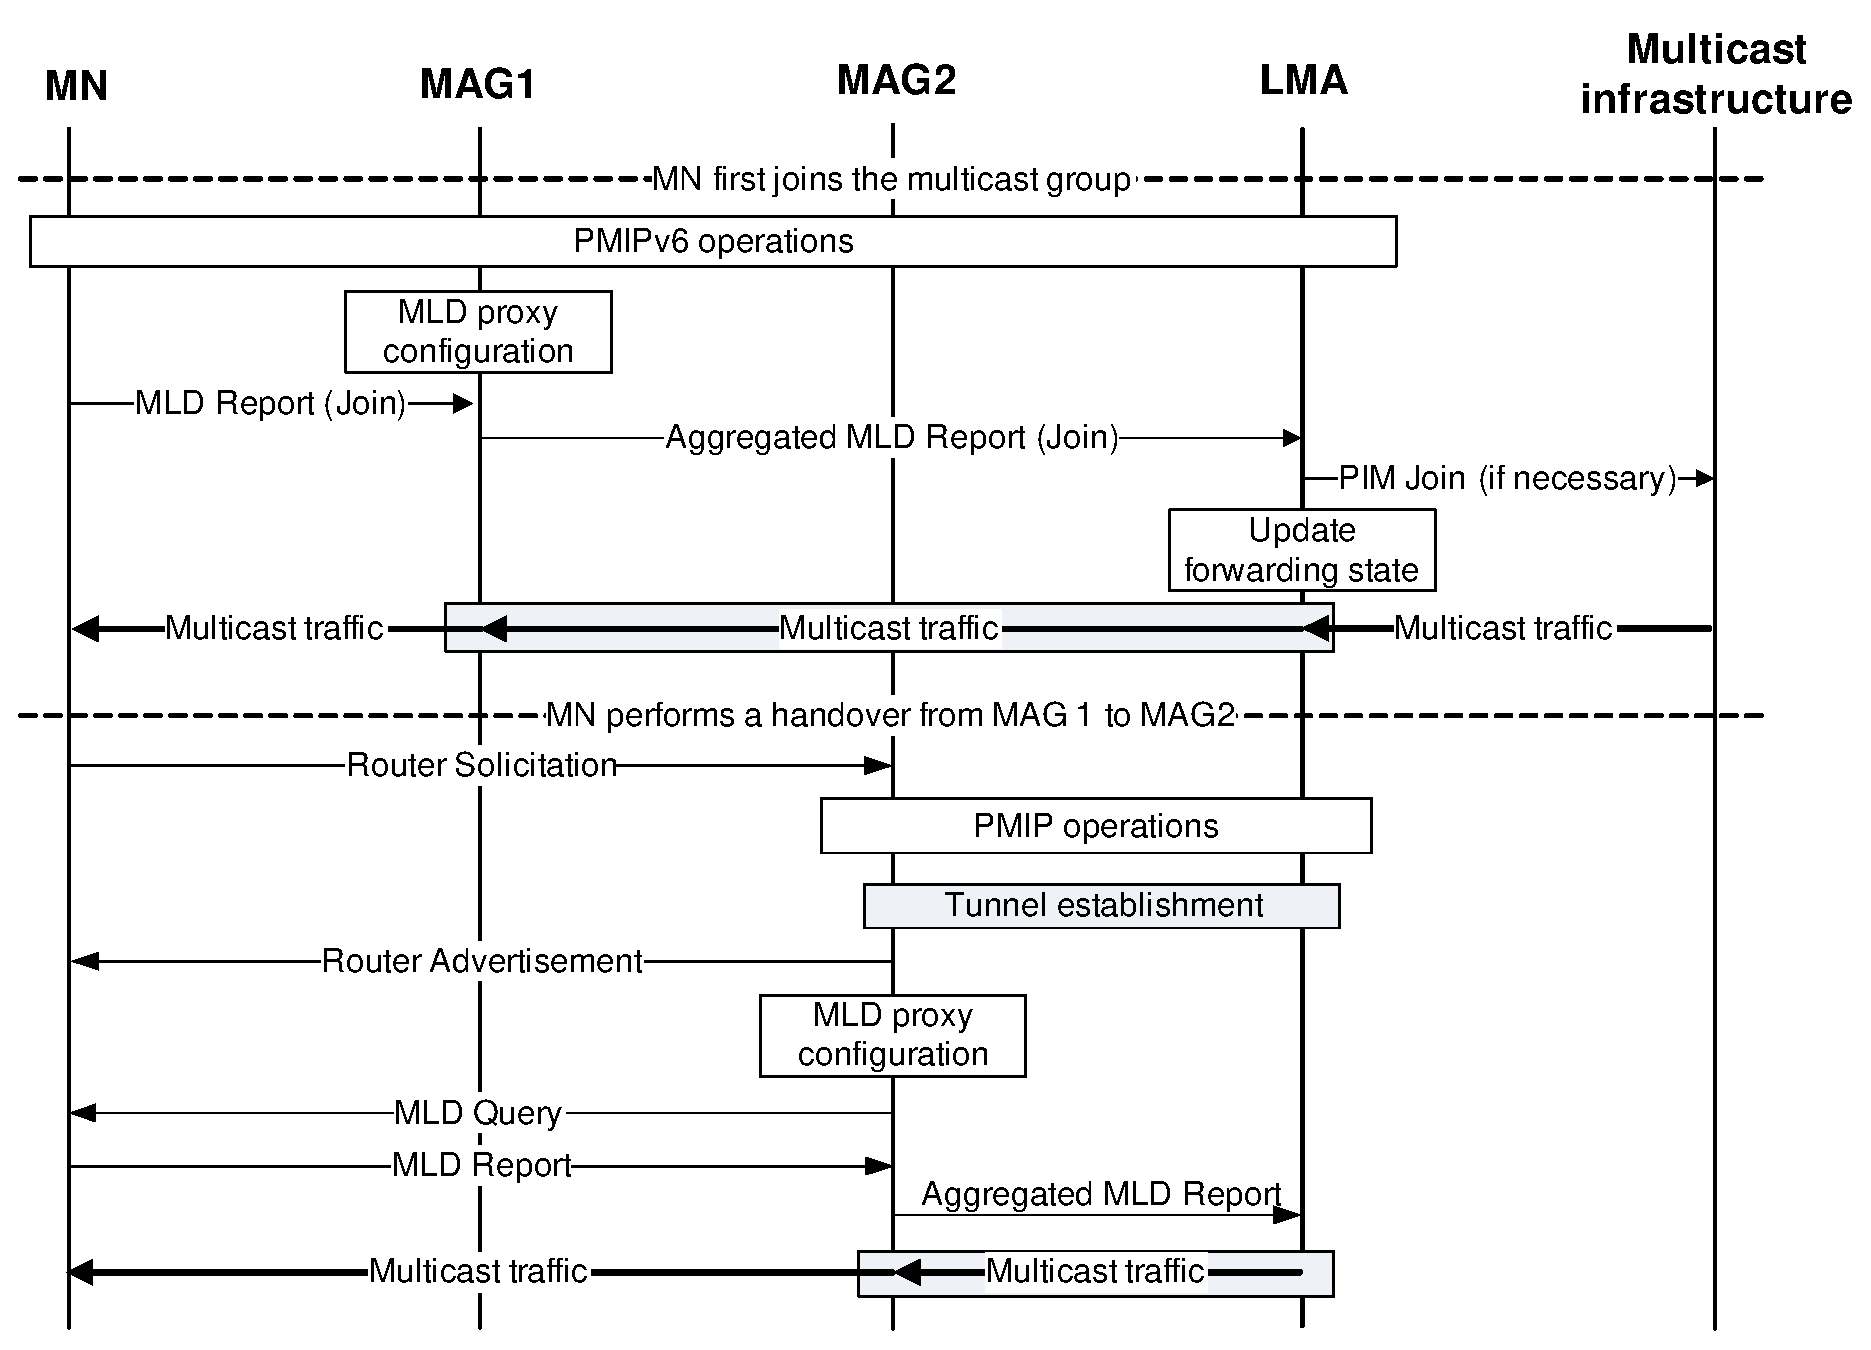
\includegraphics[width=0.85\textwidth]{./Part1/Chapter2/figures/c4_base_solution.eps} 
    \caption{Base solution for multicast listener mobility in PMIPv6.}
     \label{fig:c4_base_solution}
  \end{center} 
\end{figure} 

Fig.~\ref{fig:c4_base_solution} describes the multicast-related signaling for the base solution. When an MN is initially attached to a PMIPv6 domain (for example, attaches to MAG1), first, the standard PIMPv6 operation will be executed (e.g., MN's address configuration, MN's location update, tunnel establishment, for more details see Section \ref{c1:IP_Mobility}). MAG1 then creates an MLD proxy instance (if necessary) which serves as an upstream router for all the nodes associated with the MN's LMA. Note that every MAG-LMA tunnel is a part of a separate MLD proxy domain. The proxy instance adds the MN to its downstream interface and configures its upstream interface towards the MN's LMA. When the MN expresses its willingness in receiving the multicast traffic from a group, it sends an MLD Report to MAG1. MAG1 then sends an aggregated MLD Report message to the LMA to join the group on behalf of the MN. The LMA, acting as an MR, joins the group from the multicast infrastructure, and updates its multicast forwarding state. After receiving the multicast packets, the LMA forwards them to the appropriate MAGs according to its forwarding state (via the LMA-MAG tunnel). MAG1 forwards the packets to the appropriate downstream interfaces and they finally reach the MN. \\

In case of handover (from MAG1 to MAG2), the basic PIMPv6 operation will be executed. Since the mobility is transparent to the MN, the MN will not send the unsolicited MLD Reports. Instead, MAG2, upon the detection of a new MN on its access link, adds the MN to a downstream interface, and sends MLD General Query messages on its attached link. The MN then replies by an MLD Current State Report message indicating its current active multicast groups. Based on that, MAG2 can send an aggregated MLD Report message to the corresponding LMA to join the groups on behalf of the MN (in case MAG2 is not receiving such those multicast groups). After updating the multicast forwarding state, the LMA forwards the multicast packets to the appropriate MAGs (including MAG2). The multicast packets finally reach the MN. 

Although the base solution is a simple way to enable the multicast support in PMIPv6, it does not address any issues as specified in the previous section. In more details, the utilization of tunnel for multicast flow results in the traffic redundancy (or the tunnel convergence problem) at the MAG. It is because different nodes, which attach to the MAG and associate to different LMAs, can subscribe to the same multicast group. There are several solutions for this issue such as extending MLD proxy to support multiple upstream interfaces \cite{multi_upstream_interface}, or using the direct-routing approach \cite{direct_routing_mtma}. Also, since a lot of operations need to be executed to allow the MN to continue receiving the multicast traffic at the new MAG, it may cause a long service disruption and high number of lost packets. This issue can be mitigated by either using the context transfer from previous MAG/LMA to the new MAG \cite{d4.2,SIAL} or tuning the behavior of MLD for routers \cite{tuning_MLD}. In addition, as the multicast traffic always passes through the MN's LMA, it may cause the sub-optimal routing problem. Possible solutions for this problem can be a localized multicast traffic and using a direct routing. 

\subparagraph{Direct-routing Solution} 
In order to provide an optimal connectivity to a local content, the direct routing approach which uses native multicast infrastructure locally in a PMIPv6 domain is proposed \cite{direct_routing_mtma}. In this case, the MLD proxy is implemented at MAG in which the upstream interface is configured towards an MR in the multicast infrastructure. Therefore, the direct routing approach helps avoid the tunnel convergence problem. One of the most important advantages of this approach is that multicasting functions are totally separated from the mobility anchor by using the native multicast infrastructure. As the result, the complexity of LMA is reduced since it does not have to deal with the multicast traffic processing. In addition, this approach may not make any packet overhead (tunneling overhead) as the multicast traffic is not transferred via the mobility tunnel. However, if the tunneling mechanism is used to set up the upstream interface of the MLD proxy towards an MR, the tunneling overhead can be re-introduced \cite{direct_routing_mtma}. 

The multicast-related operation in the direct-routing approach is briefly expressed as follows. Once an MN is attached to MAG1, similar to the tunnel-based approach, a proxy instance at MAG1 adds the MN to a downstream interface and configures its upstream interface towards an MR in the multicast infrastructure. Again, when the MN expresses its interest in receiving the traffic destined to a multicast group, MAG1 sends an aggregated MLD Report message to its upstream MR to join the group on behalf of the MN. Afterwards, the multicast traffic traverses the multicast infrastructure and reaches the MN. The MN then performs a handover to the new MAG, namely MAG2. Since the MN is unaware of the mobility process, it has to wait until receiving an MLD Query to inform its multicast information state to MAG2 by means of the MLD Current State Report message. MAG2 then joins the multicast delivery tree on behalf of the MN. MAG2 has to get the multicast traffic from an MR in the multicast infrastructure which already has a multicast forwarding state for this group. In other words, the multicast delivery tree needs to be reconstructed. Thus, it may result in a noticeable service disruption and packet loss. Some mechanisms are required to make sure that the multicast session continues right after the MN is attached to the new MAG and minimize the overhead in reconstructing the multicast trees. To tackle these issues, in \cite{direct_routing_mtma}, the authors propose to use a common upstream MR for all MAGs in the domain. Additionally, MAG can implement the MR functionality, in this case, MAG belongs to the multicast-enabled domain. 

In the same document \cite{direct_routing_mtma}, the authors propose separating the multicast from PMIPv6 unicast to solve the tunnel convergence problem. In more details, the multicast tree mobility anchor (MTMA), acting as an MLD proxy or an MR, is introduced to serve as a topological anchor point for the multicast traffic. In other words, while the multicast traffic is served by the MTMA, the unicast traffic is served by the typical LMAs. Typically, the MTMA would be used to get access to the remote multicast content, while direct routing to the local multicast content. In this case, PBA message should be extended to convey dynamic policies on subscription via MTMA/direct routing. 

\paragraph{Additional Considerations \\}
In case of handover, several operations should be executed so that the MN can continue receiving the multicast traffic from the nMAG: i) Typical PMIPv6 operations (e.g., exchanging PBU/PBA, tunnel establishment and address configuration); ii) Acquisition of the MN's multicast subscription information at the nMAG: Since the mobility is transparent to the MN, the service continuity is responsible by the nMAG through joining the ongoing multicast channels on behalf of the MN. To do so, the nMAG first needs to get the active multicast subscription information of the MN. It is done by relying on the normal MLD operations or the multicast context transfer mechanism; iii) Joining and getting the first multicast packet: The nMAG then decides joining the on-going multicast channels from its upstream MR/or an additional MLD proxy. Afterwards, the MAG forwards the multicast packets to the MN. 
From the multicast service point of view, while the information acquisition operation may lead to the service disruption and signaling overhead, the joining process depending on the position and the role of the upstream MR can cause the service disruption, signaling overhead, tunnel convergence problem and tunneling overhead. Regarding the service disruption time, it depends on all the operations. However, from the multicast service perspective, only the subscription acquisition time and joining time can be reduced for accelerating the multicast delivery. As a result, there are two possible solutions for these issues. The first one \cite{SIAL, FPMIPv6_multicast, tuning_MLD, Thinh_WCNC_Multicast} aims at reducing the time for information acquisition operation. The detailed discussions on this solution will be provided in Chapter \ref{ch:multicast_PMIP}. The second one mainly focuses on reducing the time needed for the joining process. Moreover, in both solutions, the operations during handover can be executed in parallel.   

\paragraph{Solutions for Multicast Source Mobility \\}
Limited work on the multicast source mobility in PMIPv6 has been developed compared to the multicast listener mobility. From the IETF point of view, the base solution for the multicast source mobility in PMIPv6 is still under discussion. In \cite{multicast_source}, the authors suggest using the base solution for listener for source mobility. In this case, MLD proxy and MR function need to be deployed at MAG and LMA, respectively. As a proxy, the packets arriving from a downstream interface will be forwarded to all the downstream interfaces which have the subscription information of this group except the incoming one and to the upstream interface. As a result, the multicast traffic from a local source will reach all the listeners attaching to the same MAG and sharing the same LMA (serving by the same MLD proxy instance). Serving as an upstream MR, the multicast traffic will be transmitted to the LMA, which then will be forwarded along the multicast delivery trees according to the forwarding state to reach all the listeners.

After a handover, the source can continue to send the multicast packets as soon as the MLD proxy at the nMAG maps the source to the corresponding proxy instance and the standard PMIPv6 operations are completed. The detailed operation is illustrated in Fig.~\ref{fig:c4_source_base}. It is worthy to note that when the source and listeners are attached to the same MAG but associated to different LMAs, the traffic will be routed in a definitely non-optimal route from the source's MAG to the source’s LMA, passing the listener’s LMA and finally returning to the same MAG. This is called a detour routing issue. 
\begin{figure}[h!] 
 \begin{center} 
 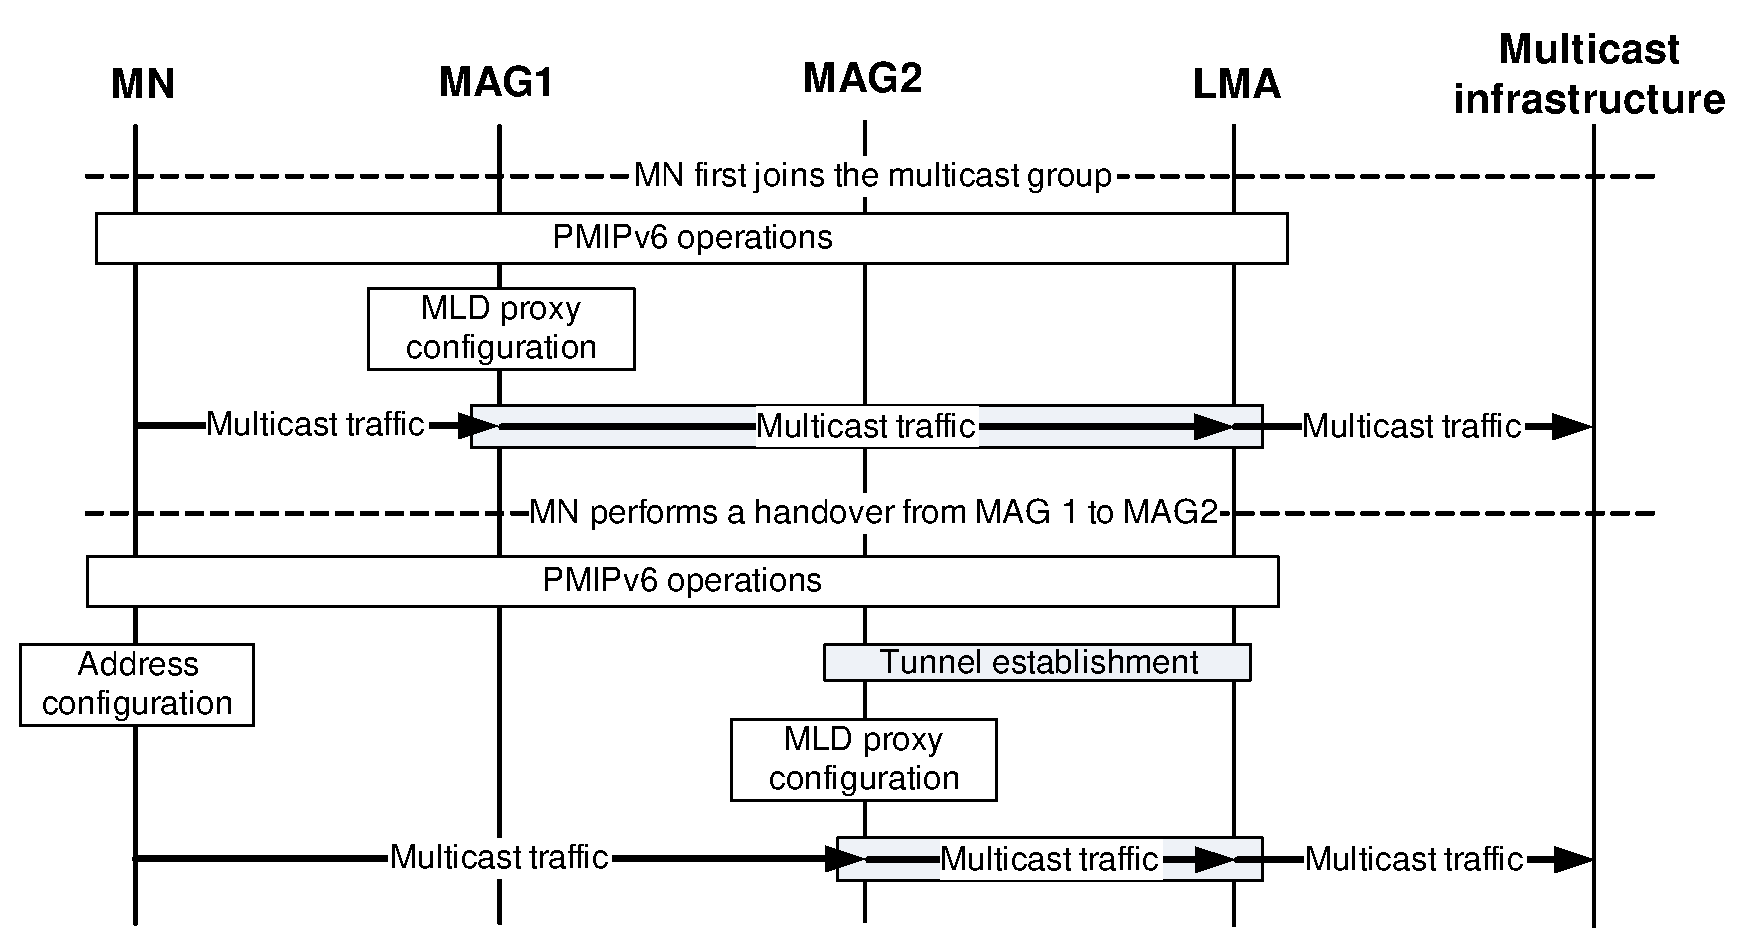
\includegraphics[width=0.75\textwidth]{./Part1/Chapter2/figures/c4_source_base.eps} 
    \caption{Signaling for the multicast source mobility support in PMIPv6.}
     \label{fig:c4_source_base}
  \end{center} 
\end{figure}

At the same document \cite{multicast_source}, the authors propose another possibility in which the multicast traffic is routed directly from MAGs to the multicast infrastructure bypassing the LMA (direct-routing). The direct routing can be supported by: i) MLD proxy deployment at MAGs with the upstream interface configured towards a common MR in the multicast infrastructure; or ii) the multicast routing protocol deployment at MAGs.  

In the former case, a single proxy instance at MAGs with the upstream interface configured to the multicast domain will serve as a first hop multicast gateway (for all the attached listeners and sources), thus avoiding the traffic duplication and detour routing. In addition, the upstream interface of the proxies should be configured towards the same MR in order to avoid the multicast tree reconstruction during handovers (which may cause significant service disruption and packet loss). The reason is when the source moves from the pMAG to a new one and if the default MRs of two MAGs are different, the nMAG's MR does not have information of this channel. Consequently, it considers the source as a new multicast source, leading to the execution of the source registering process \cite{multicast_source}. The nMAG's MR unicast-encapsulates the multicast packets and directly sends them to the RP which then sends Join messages towards the source to create the multicast delivery tree. Since the LMA acts as a global anchor point for the address of the source, the Join messages will reach the LMA which then simply discards the messages. As a result, the PIM cannot switch from phase one to phase two (or three) as it may cause several issues such as packet overhead, encapsulation/decapsulation cost, source register tunnel management and sub-optimal routing (for the listeners that are close to the source) \cite{PIM_SM}. The similar issue occurs when the multicast routing protocol is deployed at MAGs.
\subsubsection{Alternative Proposals}
Aside from IETF proposals, several research documents have been done to improve the standard multicast mobility support in PMIPv6. The purpose of these proposals is to address the performance and optimization issues such as the service disruption, the sub-optimal routing and the tunnel convergence problem. 

From listener point of view, in \cite{PMIP_listener_Li}, the authors propose two multicast listener mobility support mechanisms i.e., the LMA-based and the MAG-based, corresponding to the tunnel-based and direct-routing approach. The simulation is then conducted to evaluate the performance in terms of handover delay and signaling cost. In \cite{PMIP_multicast_fast_HO_Gohar, PMIP_multicast_fast_HO_Lee}, the authors propose the solutions based on the fast-handover approach to minimize the service disruption time and to prevent the packet loss during handovers. Again, the under link radio access technology needs to support layer-2 triggers and the solution strongly depends on the layer 2 access technologies. 

In \cite{PMIP_listener_MTMA}, the authors, following the idea of separating the management of the multicast traffic and unicast one in different LMAs (dedicated LMA for multicast traffic) in \cite{direct_routing_mtma}, provide a simulation framework to evaluate the dedicated LMA for multicast proposal. The simulation results show that this solution helps to reduce the multicast traffic load by reducing the traffic duplication.

In \cite{PMIP_listener_Seil}, the authors propose a solution similar to the direct routing approach, in which the MLD proxy is implemented at MAGs with its upstream interfaces configured to an MR in the multicast infrastructure. Then, the multicast context transfer is used to accelerate the multicast subscription acquisition at the predicted MAG. However, it may cause the issue in case of prediction failure. 
 
Limited work \cite{multicast_source_Guan_wpc, multicast_source_Wang, multicast_source_Wang_CCNC} has been done for source mobility in PMIPv6. In \cite{multicast_source_Wang}, the authors propose the solution for the multicast source mobility similar to that in \cite{multicast_source}, however, a performance evaluation is provided. In \cite{multicast_source_Wang_CCNC}, the authors extend PMIPv6 protocol to support multicast sender by introducing the Multicast Forwarding Cache (MFC) at MAG. Thus, MLD proxy functionality is not required at MAG. However, simulation is required to evaluate the performance of MFC as well as the interaction between MFC and the typical MAG functionality. 

\subsection{IP Multicast Mobility in Network-based DMM}
In DMM, there is a limited work for the multicast support since the DMM is still in an early stage of standardization. So far, no complete solution has been found for multicast in DMM. Typically, all major aspects are inherited from the problem in a PMIPv6 domain, while an additional complexity is added. It is noted that this section only presents the issues and solutions when considering a multicast mobility in a network-based DMM environment. 

Since from now on we only consider a network-based DMM environment, for simplicity, a MAR supporting network-based DMM can be called MAR, instead of NMAR in the previous section. 
We recall some abbreviations introduced in the previous chapters to denote the role of MAR from a mobile node point of view:
\begin{itemize}
\item Current MAR (cMAR, or Serving MAR (sMAR)) is the MAR to which the MN is currently attached.
\item Anchor MAR (aMAR) of an MN's address/session is the MAR where the prefix in use is allocated (and the session is initiated using this address as the source address).  
\end{itemize}
  
\subsubsection{Multicast Listener Support in DMM}
Since DMM is still in its infancy, no complete solution has been found for the multicast support in DMM. As similar in PMIPv6, the multicast listener mobility support can be enabled in DMM by deploying MLD proxy at MARs \cite{multicast_DMM_sergio, Thinh_ICNS,Thinh_VTC}. In this case, when a multicast flow is initiated, the multicast traffic is received directly from the native multicast infrastructure via the cMAR. In case of handover, the traffic is routed from the anchor to the current MAR via the tunnel between them (like the unicast traffic). In more details, when an MN subscribes to a multicast flow at MAR1, the MLD proxy instance at MAR1 sends an aggregated MLD Report message to its upstream MR (see  Fig.~\ref{fig:c4_dmm_listener_mld}). The multicast packets are then transmitted directly from the multicast infrastructure to the MN via MAR1. The MN then performs a handover to MAR2. Following the network-based DMM approach, the tunnel is established between MAR1 and MAR2 for the active flows which are initiated at MAR1. After executing the standard DMM operations, an MLD proxy instance at MAR2 adds the MN to its downstream interface, and configures its upstream interface towards MAR1 (see Section \ref{c1:IP_Mobility} for more discussions about how the MAR2 knows the MAR1 address). MAR2, after obtaining the MN's subscription information by means of the normal MLD operation, sends an aggregated MLD report to the MAR1 to join the ongoing channels. Finally, the multicast traffic is transmitted from MAR1 to MAR2 via a tunnel between them and reaches the MN. 

\begin{figure}[h!] 
 \begin{center} 
 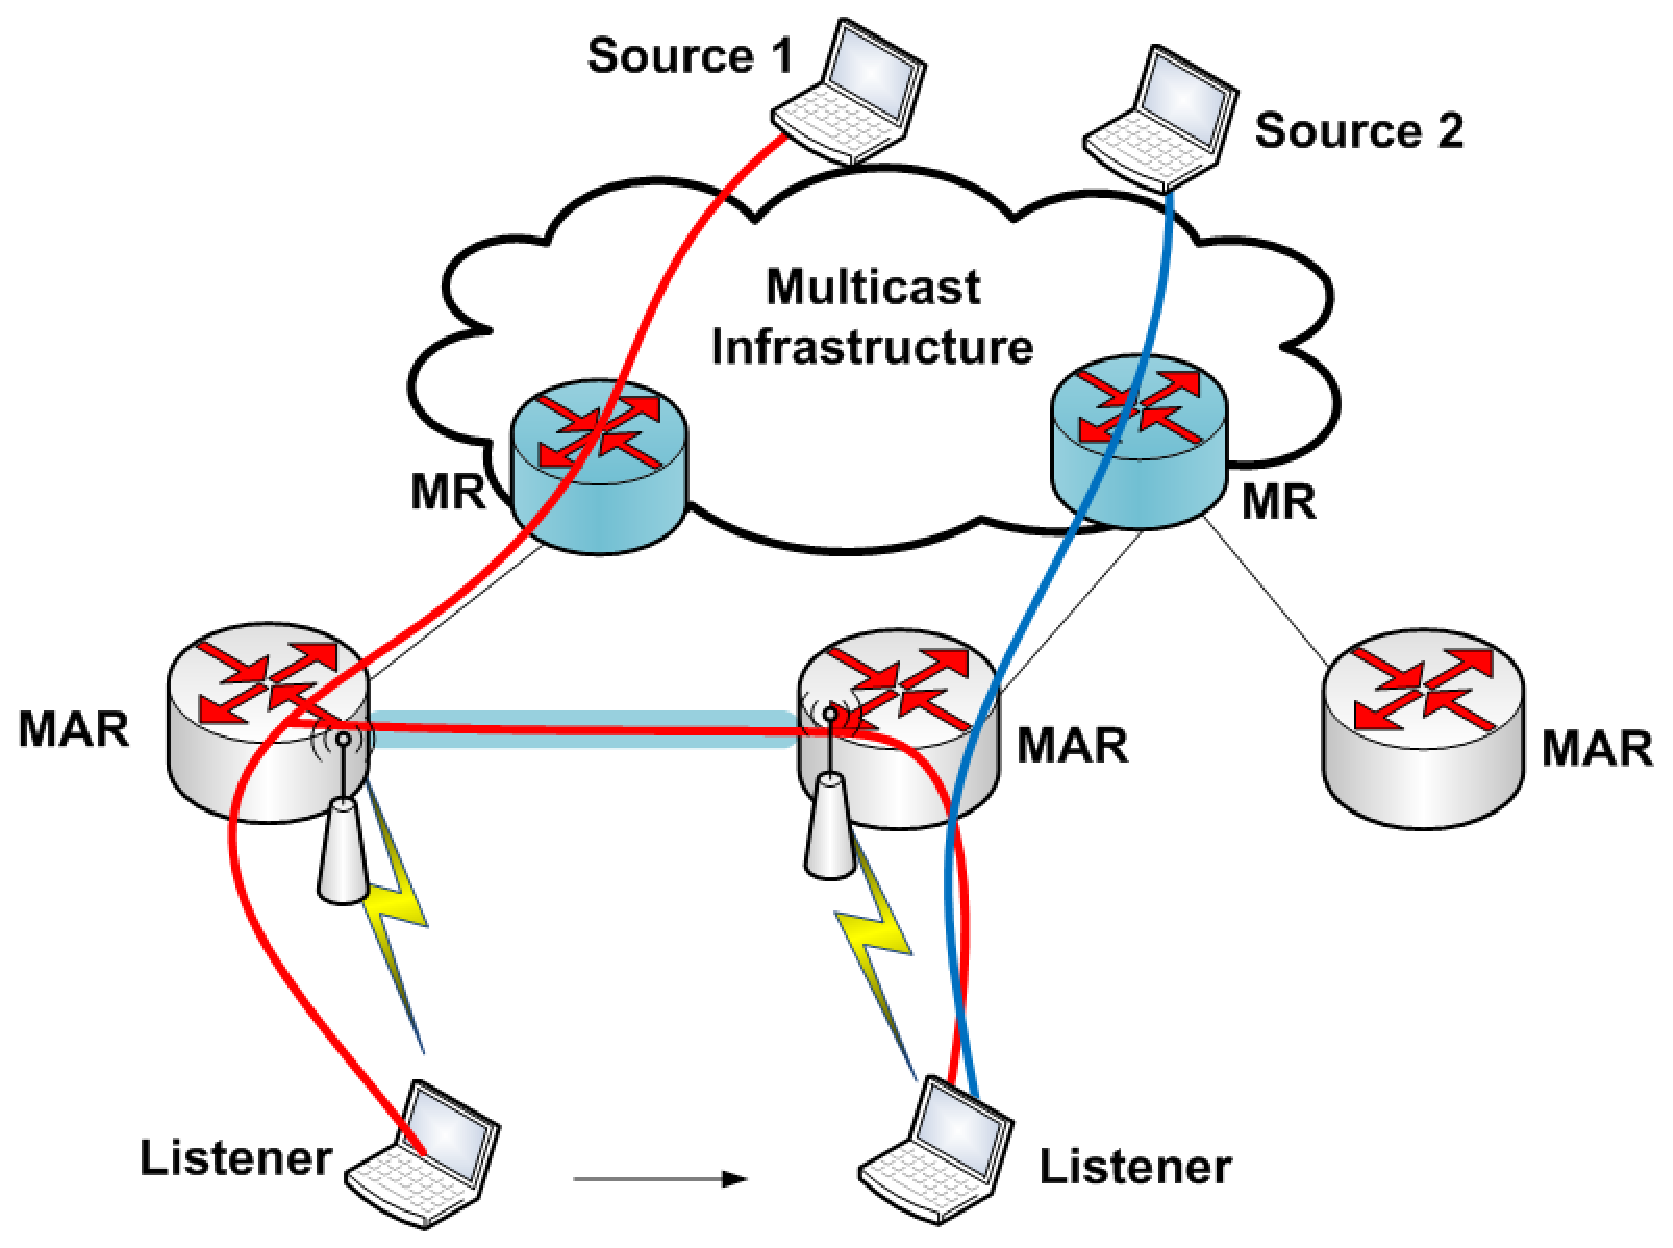
\includegraphics[width=0.50\textwidth]{./Part1/Chapter2/figures/c4_dmm_listener_mld.eps} 
    \caption{Multicast listener mobility in DMM (MLD deployment at MARs).}
     \label{fig:c4_dmm_listener_mld}
  \end{center} 
\end{figure}
However, this mode does not address any multicast-related issues. Among them, we just highlight the following issues: 
\begin{itemize}
\item \textit{Service disruption (and packet loss)}: When a multicast listener moves from the pMAR to the cMAR, several multicast-related procedures need to be executed to allow the listener to continue receiving the ongoing multicast channels. Consequently, it causes a noticeable service disruption (due to the multicast service activation, MLD response delay, and MLD Query/Report transmission). By using the multicast context transfer and the explicit tracking function, the service disruption time could be greatly reduced \cite{Thinh_WCNC_Multicast}. However, in some cases, it is far from the values required by specific services (e.g., interruption-sensitive services). For instance, in \cite{Thinh_ICNS, multicast_DMM_Sergio_PIMRC}, the authors showed that the multicast service disruption time strongly depends on the tunnel delay between the aMAR and cMAR. Hence, by reducing the tunnel delay, the service disruption time can be reduced \cite{Thinh_ICC}.
\item \textit{Non-optimal routing and end-to-end delay}: Since the multicast traffic always traverses the aMAR, it often results in a longer route (e.g., when the source and the listener are close to each other but far from the listener's aMAR). In particular, when considering a significant large domain, it can cause a high end-to-end delay. Therefore, avoiding utilization of the mobility tunnel or shortening the tunnel could help \cite{Thinh_ICC}.  
\item \textit{Tunnel convergence problem}: In case of mobility, the utilization of the mobility tunnel for the multicast flow may result in the tunnel convergence problem. This issue occurs when multiple instances of the same multicast traffic converge to an MAR, leading to the redundant traffic. It is because the multiple MLD proxy instances are installed at the MAR with their upstream interfaces configured to different aMARs. Since the purpose of DMM is moving the mobility anchors from the core to the edge of the networks, the number of mobility anchors in a DMM domain will be much more than that in a PMIPv6 domain. As a consequence, the tunnel convergence problem is supposed to be much more severe than that in PMIPv6, especially in highly mobile regimes. As stated in the DMM requirements \cite{DMM_requirements}, the multicast solutions in DMM should take this issue into consideration. In \cite{Channel_manageable_Seil}, the authors introduced a framework managing all multicast channels and controlling which channel should be received from the multicast infrastructure (for local content) or the previous MAR (for remote content). This solution helps to minimize the multicast traffic duplication. However, as only one upstream interface is configured at a time, it may cause the tunnel convergence problem again when an aggregated MLD Report is sent to the upstream interface. Thus, the tunnel convergence problem cannot be completely avoided. On the other hand, the problem can be solved by using an extension to MLD proxy to support the multiple upstream interfaces \cite{multi_upstream_interface}. In this case, only one proxy instance will be installed at MAR with different upstream interfaces towards different aMARs (and its upstream MR). Hence, the MAR will receive only one instance of the multicast packet. Also, in a DMM environment, it is unfeasible to pre-establish all the tunnels between MARs since the number of MARs is supposed to be large. When considering the MLD proxy supporting multiple upstream interfaces in DMM, it may cause the complex tunnel management (e.g., maintenance of the tunnel and keep alive signaling). Another solution which helps to reduce the number of duplication traffic is proposed in \cite{Thinh_ICNS}.
\end{itemize}

Considering the MR function deployment at MARs, the MAR will decide to get the multicast traffic from an MR for an attached listener based on the Reverse Path Forwarding (RPF) check. As a result, the tunnel convergence, non-optimal route will be avoided. However, the movement of the listener causes the service disruption problem. Additionally, the operators may not want to support the multicast routing function on MAR due to its implementation and operational costs compared to MLD proxy.

\subsubsection{Multicast Source Support in DMM}
Similar to the multicast source mobility in PMIPv6, a limited work has been done for the source mobility in PMIPv6. Also, multicast source mobility in DMM inherits the issues from that in PMIPv6. In \cite{d4.2,multicast_DMM_sergio}, the authors propose to enable the multicast source mobility in a DMM environment by deploying MLD proxy at MAR. In case of handover, the multicast traffic will be routed from the current MAR to the anchor one via the mobility tunnel between them. Although this solution is simple and easy to deploy, it comes up again the sub-optimal routing when the source and listeners, after handover, are attached to the same MAR (but from different anchor MARs). When the MAR acts as an MR, it considers the source as a new source. Thus, it encapsulates the multicast packets and sends them to the RP (in case of ASM). The RP then sends a PIM Join message towards the source's aMAR to establish the SPT. Thus, the traffic first passes the aMAR and then the RP. In addition, if the mobility occurs after the DR's listener switches to the SPT towards source, the mobility will reset the SPT routing state, leading to a significant service disruption and packet loss. In case of SSM, the multicast delivery tree will be reconstructed based on PIM process. Again, it may cause a noticeable service disruption and a high number of lost packets. 
\section{Conclusion}

As more and more applications and services in the Internet are based on the multicast technique, the multicast will play a crucial role in the future networks. So as to provide the multicast service, two groups of protocol need to be deployed: the multicast group membership protocols and the multicast routing protocols. The multicast group membership protocols are used to communicate between the hosts and their routers. Relying on MLDv2, we analyzed the role and operations of these protocols. Using MLDv2 protocol, a host informs its router about its interest of receiving/leaving a multicast group, while an MR manages its membership state information on the attached link. Various multicast routing protocols then have been presented, in which the PIM-SM protocol is insisted. Finally, to avoid deploying a full-stack multicast router in a given network, an MLD proxy is introduced as a lightweight solution. 

Regarding IP mobility management protocols, there are a various IP mobility protocols ranging from the host-based to the network-based, from the centralized to the distributed approach. Typically, PMIPv6 as a network-based mobility management offers advantages compared to the host-based one in terms of complexity of the MN, signaling overhead and handover latency. However, PMIPv6, as a centralized mobility approach, relies on a centralized mobility anchor to support mobility. Thus, it causes several limitations when the number of mobile devices and their traffic demand increase. To tackle these limitations, DMM has been introduced. The research publications showed that DMM is a promising choice for the future networks. 

Based on the analysis regarding IP multicast and IP mobility management protocol, we then highlighted the issues when considering IP multicast in different mobility management protocols. First, we have made a brief introduction on the multicast-related issues as well as the proposals for multicast mobility in MIPv6. We then made an in-depth analysis in PMIPv6 and DMM. In the context of our thesis, we focus on such issues as the multicast service disruption, packet loss, sub-optimal routing, tunnel convergence problem, and leave latency (waste of resources).  
 

\chapter{Related Works}
\label{ch:performance_evaluation}
\section{Interoperation in IoT}
\section{Data Quality Enhancement in IoT}
% \section{Introduction}
% \section{Data Outlier}
% \subsection{Definition of data outlier}
% \subsection{Impact of outlier in IoT}
% \subsection{Outlier detection}
% \section{Data Cleaning}
% \subsection{Anomaly detection techniques}
% \subsection{Change point detection techniques}
% \subsection{Open challenges}
% \section{Conclusion}


\chapter*{Conclusion of Part \ref{pa:part1}}


\part{Interoperation in IoT}
\label{pa:part2}
\chapter*{Overview of Part \ref{pa:part2}}
...... To be complete.............

\chapter{An Industrial IoT Framework to Simplify Connection Process using System-Generated Connector} 
\label{ch:connector} 
\section{Introduction}
The Internet has fundamentally transformed the way humans interact. Over the next decade, the Internet of Things (IoT) will revolutionize manufacturing, energy, agriculture, transportation and other industrial segments of the economy which are estimated to be in the range of \$2.7 - \$6.2 trillion by 2025~\cite{manyika2013disruptive}. This significant development accompanies with the increase in equipment manufacturers, Internet service providers, and application developers. By the end of 2020, 212 billons IoT smart objects are expected to be deployed worldwide~\cite{gantz2012digital}. Machine-to-Machine (M2M)\index{M2M} traffic flows will constitute up to 45\% of the whole internet traffic in 2022~\cite{taylor2013next},~\cite{evans2011internet}. Additionally, the Industrial Internet (IIoT, Industry 4.0)\index{IIoT} is predicted to create about 1279 billion dollar in 2020 according to Wikibon report~\cite{floyer2013defining}.\\

While Industrial IoT offers infinite potentials and opportunities for current industries and their process transformation, achieving interoperability is still a major challenge due to lack of uniform standards. One of the emerging technologies to overcome this challenge is IoT middleware. It is a software system implemented as a middle layer between device and application layers. The IoT middleware provides a set of programming abstraction to cover the heterogeneous things and low-level communication between IoT devices and end-user applications~\cite{fersi2015middleware}. Global Sensor Network (GSN)\index{GSN}, Xively, Paraimpu, ThingWorx are some of the major middleware solutions used in similar context. These systems share a common objective of achieving seamless integration of heterogeneous things into the Internet with different approaches. For example, GSN uses a concept named wrapper to handle the connection from sensor hardware to middleware. Hydra, ThingWorx offer a Device Development Kit to create the applications on device side. However, these approaches require programming skill and a lot of effort to establish and configure connectivity for new IoT object, which do not appropriate for non-specialist users. In case of GSN, in order to establish the connection from sensors to middleware, we must build an executable file named wrapper and a corresponding configuration file for every sensor using provided library. \\

Due to heterogeneity in IoT environment, each IoT object such as sensor and actuator provides different software interfaces and communicating configuration to exchange data and control information with cloud-base middleware. Furthermore, these interfaces and configuration are non-standardized and frequently changing, expecially in a Low Power Wide Area Network (LPWAN) senario. Moreover, to retrieve the monitoring data from IoT devices using LoRa  connection, we have to configure an HTTP callback following special format which is defined by a network provider. However, each provider has various configuration formats and frequently changes that lead to a giant gap in syntactical interoperability and stability.\\

In the IoT era, data processing plays a tremendous role in analysis, prediction and context-awareness. Along with the exponential growth of the open data services (ODS), interoperating between these services and IoT middleware is challenged by heterogeneity. Most of the ODS follow a client-server model built using RESTful web service. However, each service provider offers a diverse HTTP configuration (path, method, header), data format (JSON, XML) and data syntax. For examle: ``Accuweather'', a weather data sharing service, configures identification key as a parameter in the URL namely ``apikey''. However, ``Openweather'' service configures identification key in the HTTP header. Therefore, a new mechanism to deal with heterogeneity syntax of IIoT connectivity should be considered.\\

In this chapter, we present a novel Industrial IoT framework to support automatic establishment and configuration process for heterogeneous connectivity by using a system-generated connector. The connector is a specific code segment that performs the data acquisition process from a specific type of connection using protocols like HTTP, MQTT. Our framework also provides APIs to perform full ``create, read, update, delete'', CRUD operation on the connectors. Furthermore, automating connectivity mechanism assists end-user in quickly retrieving data from various data sources via self-defined connectors. These connectors also allow explicitly specifying the information to be collected. For example, we can create a connector to retreive only current temperature and humility amongs deverse data of open weather data sources. Thus, this mechanism enables the middleware to accelerate data acquisition process. Especially, our proposed framework is extremely fit for LPWAN scenario which lacks of uniform data and interoperation between network provider. Moreover, sensing data of LPWAN devices is restricted due to low data rate and bandwidth. Thus, enriching data from open data sources is extremely necessary for this scenario to gain maximum benefit from data analysis and context-awareness. To demonstrate the capability of this framework, we integrated it into an existing middleware to evaluate the performance. \\

The main our contributions are:
\begin{enumerate}
    \item Identifying current middleware limitations for connectivity and automatic configuration for IIoT.
    \item Proposing a novel and lightweight framework to accelerate the connecting process for heterogeneous things.
    \item Utilizing the proposed framework to speed up the data acquisition from open data sharing web services.
    \item Simplifying connectivity management by wrapping connectivity object in a RESTful web service.
    \item Implementing and evaluating the proposed framework.
\end{enumerate}

\section{Related Work}
In this section, we review the connectivity mechanism for IoT device in some current frameworks. We also identify their limitations to motivate to deliver a novel IIoT framework that simplifies the establishing and configuring connectivity to IoT things using the system-generated connector.

\begin{description}
    \item [FIWARE] is cloud-based middleware platform that provides an infrastructure to effectively reduce the cost of creation and delivery IoT services by sharing and re-using Generic Enablers (GE)~\cite{zahariadis2014fiware}. All API and GE specifications are public and royalty-free for all developer. These documents contain the necessary information to create an IoT product that can interoperate with other developed GE in FIWARE community. The other innovative aspect of FIWARE is that all IoT things are covered behind OMA Next Generation Service Interface (NGSI) entities. Therefore, developers just need to learn and work with the NGSI API used in FIWARE regardless the complexity of IoT technologies and deployment. To handle messages from the IoT devices and gateway, FIWARE provides an element namely IoT Agent. The main responsibility of this element is receiving and translating the messages to a uniform format. Currently, FIWARE IoT Agent supports HTTP and MQTT~\cite{iota-fiware-iot-stack}. However, creating a new IoT Agent involves a lot of effort to understand the FIWARE framework  which is only used by developer. Regarding integration with data sharing service, FIWARE proposes Cygnus, a connector between Orion Context Broker to certain FIWARE storage such as CKAN, HADOOP, DynamoDB. Cygnus is based on Apache Flume  which supports collecting data via persistence agents. Basically, Cygnus only supports some specific HTTP Flume agents. That means, FIWARE is able to integrate with a few supported data sources.
    
    \item [Global Sensor Network] is a platform aimed to provide a flexible integration with different type of sensors. GSN facilitates the connecting process of heterogeneous sensor devices to an application by implementing a corresponding wrapper and an XML file~\cite{Aberer2006}. This XML file defines the basic configuration information for the sensor such as the type of data will be sent to GSN, parameters, and the corresponding wrapper. The wrapper acts as a sensor driver to establish a connection from sensor hardware to GSN. These two elements must be created for every sensor which demands to connect to GSN. Currently, creating the wrapper and establishing the connectivity are complicated tasks and require high programming skill~\cite{gsn_2013}. Another critical drawback of GSN is that all sensor data is stored in an SQL database. This leads to a limitation in performance and scalability.
    
    \item [Hydra] Hydra middleware project aims to develop a service-oriented middleware for physical devices in a distributed architecture, also known as Link Smart~\cite{eisenhauer2009development}. This framework is developed based on Service Oriented Architecture (SoA), which uses web services for seamless integration of heterogeneous physical devices into applications regardless connectivity technologies. Hydra also provides a dedicated access control mechanism to ensure the authorization and privacy for all IoT services and devices. The Hydra IoT devices are described by using semantic technologies. Thus, the new devices can be discovered automatically in the Hydra Network using peer-to-peer network technology. Hydra also provides the set of development resource to create an application on both device and end-user side including the Software Development Kit (SDK) and the Device Development Kit (DDK). But, both SDK and DDK are complicated to be used by end-user. In addition, creating a new device template or Hydra IoT Application must be implemented by a programmer. Therefore, this middleware is not suitable for the end user to quickly create or deploy the IoT devices, services or applications. The other limitation of Hydra is that the Hydra device application interacts with middleware using web service. Thus, this application is too heavy to run on constraint IoT devices which limit to memory size and processor.
    
    \item [Kaa] Kaa project is open-source IoT middleware platform with a lot of IoT features that allow the users build the complete end-to-end IoT solution including data management, data connection and configuration management~\cite{kaa_project}. Kaa middleware uses data scheme and configuration scheme to configure IoT devices in term of data structure and device configuration. These schemes are created and managed by Common Type Library (CTL). It also provides a SDK to create the embedded application for IoT device in several programming languages such as C, C++, java and Objective C. However, the limitation of Kaa middleware is that the endpoint SDK only supports few specific IoT devices and the interoperation with other data sources is not mentioned.
    
    \item [Xively] is a cloud-based platform using a central message bus to route the message from devices to another platform components. This platform provides many development tools and resources supporting developer connect and obtain data from their sensors. The IoT sensors can connect to Xively via MQTT, HTTP and Web Socket protocol~\cite{kohler2014platforms}. However, the principal purpose of Xively is just to simplify the connecting from the sensors to Xively’s Cloud. Therefore, in case we need an additional service, we need to develop a new one or reuse compatible service with Xively. Adding a new sensor to Xively is supported to be uncomplicated, but the provided API is hard to use, especially for the unsupported sensor. Furthermore, there is no the function using to integrate with open data sources via web service. These limitations lead to the restricted usage for inexpert users.
    
    \item [ThingWorx] ThingWorx platform addresses IoT application integration that monitors, manages and controls connected devices through model driven development. All sensors, applications, and services are treated as data sources and inter-connected via virtual bus~\cite{derhamy2015survey}. The platform supports several connection protocols including CoAP, MQTT, REST/HTTP and Web Socket. It also supports integrating with other sharing data sources via web services including open weather services, social data providers. However, ThingWorx only supports a few web services, and not allow the user to establish the integration to new web service. The other limitation of ThingWorx is that devices only allow connecting to ThingWorx’s Cloud by using the applications to be implemented by ThingWorx SDK~\cite{solutions25platform}.
    
\end{description}

\section{Problem Statement}
 Most of the studied platforms limit the type of sensor that can be connected and request a specific application installed on device side. Also, adding a new sensor to the platforms is complex and require advanced programming skills. There is no mechanism to deal with the rapid changes things in term of software interface, connectivity protocol and data format. Moreover, reviewed frameworks do not support the end-user to establish connection and collect data from open data sources via HTTP, MQTT, CoAP or WS protocol. Our framework has been designed and developed to overcome with these limitations.
 
 
\section{IoT Framework for Connectors}
This section concentrates on our middleware architecture, connector management mechanism and connector generation process along with its elements. At the end of the section, we describe different deployment scenarios to emphasize its high compatibility with various parts of IoT system.

\subsection{System Architecture Overview}

\begin{figure}[h!] 
 \begin{center} 
 \includegraphics[width=0.72\textwidth]{./Part2/Chapter4/figures/connector_architecture.png} 
    \caption{The overview of framework architecture.}
     \label{fig:c4_overview_architecture}
  \end{center} 
\end{figure}

Our framework simplifies the creation and management process for heterogeneous connectivity. Our approach is to wrap the complex establishing and connecting functionalities in the RESTful web services which are easily handled by end-user. Fig.~\ref{fig:c4_overview_architecture} depicts the proposed framework which is composed of three different layers described below.
\begin{itemize}
    \item \textbf{Service Enablement Layer:} This layer consists of several web services which allow the end-user a direct interaction with the framework. The supported operations are (i) discovering connector, (ii) CRUD operations on connector and connector template, (iii) activating, de-activating connector and (iv) access control based on session token. There are four main services are connector management, connector discovery, access control and connector template management. These services allow the end user to establish and manage connectivity to IoT devices as well as various data source simply regardless the complexity of protocol and configuration process through RESTful web service. This capability is essential and important for adapting to the lack of standardization and the rapid changes of IoT thing. However, it is not supported by the reviewed IoT platforms.
    \item \textbf{Processing and Storage Layer:} This layer contains the databases and primary functions to generate the connectors as well as pre-process data. It also carries a database to store generated connector, connector template, and connector status. The connector creation process is performed and managed by connector generation service. This service generates the connector from connector template which is configured and sent by the end user via connector management service.
    \item \textbf{Connection Layer: } This is composed of many generated connectors that have the responsibility to handle the connection to IoT things. Currently, our framework supports two types of connectors - ‘Connector In’ and ‘Connector Out’. They are analogous to ‘proxy-in’ and ‘proxy-out’ concepts introduced in~\cite{datta2014iot}. Each type of connector supports HTTP, MQTT, CoAP and WebSocket (WS) connectivity respectively to retrieve data from sensor, actuator, gateway and open data sharing services. This is extending the ``collection proxies'' concept presented in~\cite{datta2016easing}. This layer also keeps tracking the connector status via connector management module. The end user can manage this status by calling the appropriate web service. 
\end{itemize}
\subsection{Connector Generation Elements}
To facilitate the connectivity generation for end-user, we propose the Connectivity Configuration Template (CTT) file, contains the vital information of seeking connectivity such as connection properties, data description. This file is encoded under XML format which provides simplicity, openness, and extensibility. The CTT’s content is coherent and convenient for both human and machine. Moreover, the structure of CTT is roughly equivalent to a network packet corresponding to the supported connection. Fig.~\ref{fig:c4_connector_operation} illustrates an example of complete CTT file to establish an HTTP connection to acquire the data from Accuweather, an open data sharing service about weather information.\\

\begin{figure}[h!] 
 \begin{center} 
 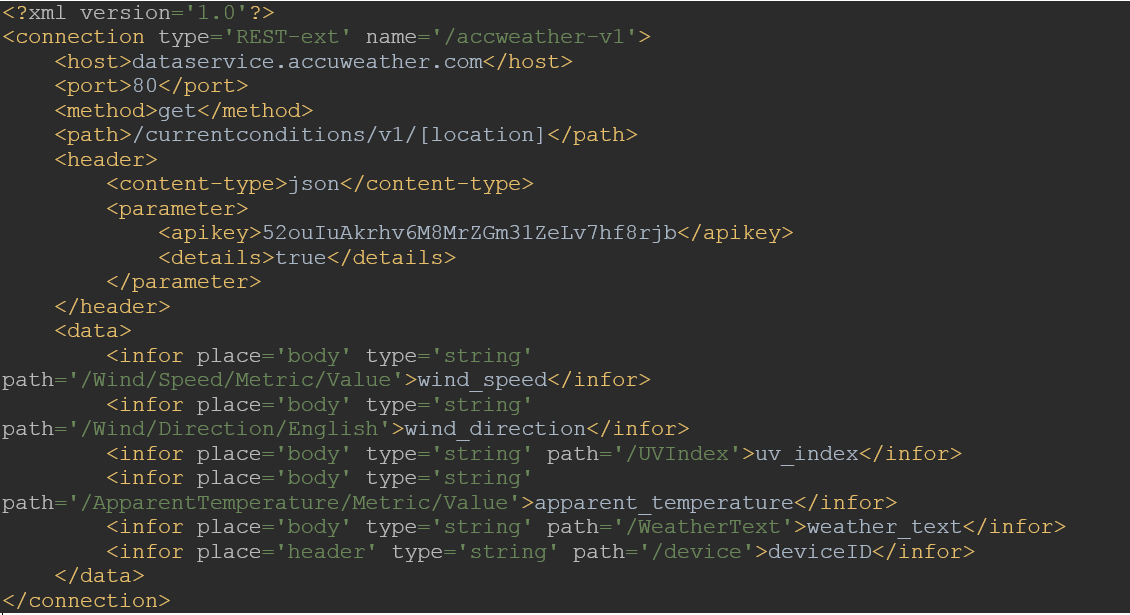
\includegraphics[width=0.72\textwidth]{./Part2/Chapter4/figures/connector_template.png} 
    \caption{An example of Connection Template.}
     \label{fig:c4_connector_template}
  \end{center} 
\end{figure}

From Fig.~\ref{fig:c4_connector_template}, the necessary connection properties are a host address, port number, connection method, path address. The header element defines the operating information of HTTP transaction such as content type, authentication information and HTTP parameters. The next element describes the carrying payload in the HTTP packet. Each data in the payload is defined by one ``infor'' tag that has three attributes including (i) ``place'' which describes the HTPP object storing the payload such as HTTP body or HTTP header, (ii) ``type'' which describes the type of the data such as string or number, (iii) ``path'' which defines a specific location of data in the payload.\\

The connector is a piece of JavaScript code, which has a responsibility to open connectivity and perform data acquisition. It is also able to annotate the raw data by using define vocabulary which increases the interoperability. The connector structure consists of three distinct parts with the different responsibility to (i) open the connection based on the received in the CTT file, (ii) de-capsulate and process the data from the received network packet and (iii) manage the connector status via web service. The connector functionalities are not only triggered by incoming network packet but also by defined interval time to obtain data from open data sharing services. In order to facilitate the management process, the framework uses a brief and a unique name to identify connector. In case multiple devices connect to the same connector, these devices are identified by their ID. The position of device ID is configurable in connector. For example, in Fig, 2, device ID will be retrieve via ``device'' parameter in HTTP header. The connector is created by combining CTT and Connector Template (CT). CT is a composed script with the marked position which is filled by the extracted information from CTT to create the connector. Each type of connector has different CT.

\subsection{The Framework Process}

The primary task of our framework is presented in Fig.~\ref{fig:c4_connector_general_operation}. In order to create and effectively manage the connector, the end-user must follow these steps. Firstly, they send the connectivity protocol used (e.g., HTTP, MQTT) to the framework via RESTful web service and then the framework response a CTT file corresponding with their demand. Secondly, the end-user fills received CTT file with connectivity configuration information such as host address, port number and send this CTT file to framework to trigger the connector generation process. Finally, the framework automatically generates the connector base on CTT file from user and response generating status along with connector name to the user. After generating, this connector is available to receive or obtain data from IoT things as well as be managed via web services.

\begin{figure}[h!] 
 \begin{center} 
 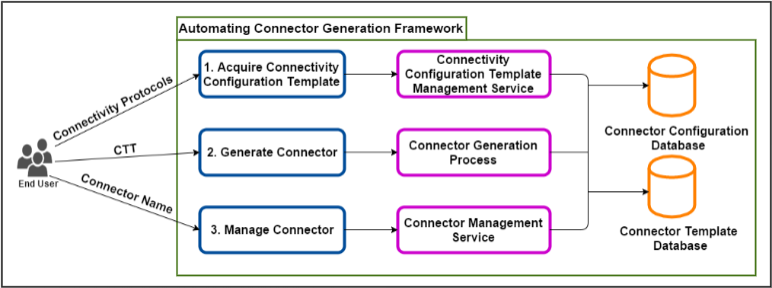
\includegraphics[width=0.72\textwidth]{./Part2/Chapter4/figures/connector_general_opereration.png} 
    \caption{The framework in operation}
     \label{fig:c4_connector_general_operation}
  \end{center} 
\end{figure}


\subsection{Connector Generation Process}
The connector generation is triggered when receiving a creating connectivity requisition from end-user via Service Enablement Layer. This request carries the CTT file which contains the necessary configuration to establish connection encoding under XML format. CCT can be delivered to end-users in advance by RESTful web service to supports the non-specialist end-user in creating connectivity. The framework extracts the vital information in received CTT and assigned this information to an array following a certain order. The next operation is to inject these values into the correct positions in CTT file. After successfully creating, the new connector is stored in database and register with connection layer to be available. The overall process is illustrated in Fig.~\ref{fig:c4_connector_operation}.

\begin{figure}[h!] 
 \begin{center} 
 \includegraphics[width=0.72\textwidth]{./Part2/Chapter4/figures/connector_operation.png} 
    \caption{The operational diagram.}
     \label{fig:c4_connector_operation}
  \end{center} 
\end{figure}

\subsection{Connector Management}
In order to control the connectors from end-user, we propose Connector Management Component (CMP) which is located in Connection Layer. CMP manages all existing connectors following Resource Oriented Model.  Each connector is identified via unique connector name which allows connector resources to be discovered by ``Connector discovery'' component in Service Enablement Layer. \\

At first declaration, the framework will automatically register the new connector with CMP by its name. After successful registration, CMP will allocate a set of RESTful web services to registered connector. Our framework supports basic management actions on a connector including CRUD, activation and deactivation. For instance, after successful creating, a connector is associated with ``active'' status and ready for operating. The end-user can deactivate the connector by triggering ``deactivate'' action.
\subsection{Deployment Scenarios}
Our framework is implemented using Node.js programming language, a JavaScript runtime built on Chrome's V8 JavaScript engine using an event-driven, non-blocking I/O model~\cite{joyentnodejs}. Therefore, it is extremely lightweight to be efficiently deployed in the wide range of the M2M objects such as a gateway, cloud-based system and even smartphone. This capability makes the framework are flexible to integrate into various parts of IoT ecosystem. For a large-scale enterprise using various technologies to communicate, our framework can be deployed to the gateway to facilitate the connection process for new devices and easily adapt to the changes of configuration from network providers and new coming connectivity standard. In the real scenario, the framework is deployed in a cloud-based system using to simplify connectivity to devices via LPWAN connectivity. In the other perspective, our framework can be implemented as a data acquisition layer in other frameworks such as SIGHTED~\cite{nagib2016sighted} or as a proxy layer in a lightweight Framework for efficient M2M device management in oneM2M Architecture~\cite{datta2015lightweight} to accelerate the connection process.


\section{Evaluation}

To evaluate our framework, we propose to measure the execution time of connector generation process including two main operations, namely connector creation and reloading framework

\begin{itemize}
    \item \textbf{Connector creation operation: } The operation performs the combination of CTT uploading from end-user and CT storing in the database to generate the target connector.
    \item \textbf{Reloading framework operation: } After the finish of connector generation process, this operation occurs to integrate new connector into the framework.
\end{itemize}

We recorded the execution time in seconds of 50 times wrapper generation process with the wrapper configuration is 852 bytes. The evaluation is performed on-device has the processor: Intel(R) Core(TM) i5-6200U CPU @ 2.30 GHz, 2401 MHz, 2 Core(s), 4 Logical Processor(s), 4 GB of RAM and the operating system is 64-bit Windows 10. The acquired result is shown in Figure 6. According to that, reloading framework takes around 1.15 s to 2.91 s while the connector creation operation only consumes around 0.113 s to 1.4 s. Overall, the total execution time is from 1.265 s to 4.31 s. This performance satisfies the user experiment~\cite{rosson2002usability}. When the connector works as a ``proxy out'', the time of establishing connection is extremely minor around 0.003 ms comparing with the total time which is largely depended on the performance of the data sources. In addition, most of open data sources are limited in the performance and the number of request could be served per second. \\

\begin{figure}[h!] 
 \begin{center} 
 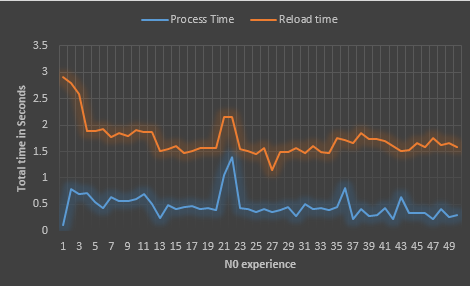
\includegraphics[width=0.72\textwidth]{./Part2/Chapter4/figures/connector_performance.png} 
    \caption{Connector generation performance}
     \label{fig:c4_connector_performance}
  \end{center} 
\end{figure}

The size of connector for each M2M connectivity is less than 1 KB, and the requested memory of our framework is only a couple of megabytes of memory. Thus, our framework is satisfactory to deploy on the general IoT objects from cloud-base middleware, M2M gateway and event smartphone with gigabytes of internal memory along with the powerful processor. It further demonstrates the ultra-lightweight of the proposed framework. In the other hand, the size of CTT only depends on the data section. However, this section is not processed or participated in connector generation process. Therefore, the performance of connector generation process is independent of the size of CTT. Furthermore, the connectors are developed Node JS Express framework  supporting non-blocking I/O model, and consequently, there is unlimited in the number of devices connecting to a connector. These properties make the framework more scalable and flexible to be deployed in the large-scale scenario.

\section{Conclusion}
In this chapter, we identify the limitations of some existing middleware solutions regarding the data acquisition and configuration connectivity. Motivating to bridge the gaps, we proposed a framework that can simplify the establishing connection process from IoT things to cloud-based middleware via a system-generated connector. Our platform also provides well-supplied management web services based on resource oriented model. It allows the end users to easily discovery and perform a wide range of management operation on the connector including creating, retrieving, updating and deleting as well as activating or de-activating. Another innovative aspect is that the connector can facilitate and speed up the data acquisition process from data sharing web services such as Accuweather, OpenSensorIO. In evaluation section, we demonstrate the scalability and flexibility of our platform via satisfactory performance, lightweight software implementation and low memory consuming. Regarding future works, we are working on integrating our platform into oneM2M architecture and implementing access control mechanism.



\chapter{A Scalable IoT Framework to Design Logical Data Flow using Virtual Sensor} \label{ch:VSF} 
During recent years, we have witnessed an explosion on the Internet of Thing in term of the number and types of physical devices. However, there are many limitations of these devices regarding their computing power, storage, and connection. They affect on-device processing of sensed data significantly. Centralized treatment of IoT data has proven challenging for many use cases demanding real time response. This chapter aims at augmenting sensor data processing using the concept of virtual sensors. We propose a scalable virtual sensor framework that supports building a logical data-flow (LDF)\index{LDF} by visualizing either physical sensors or custom virtual sensors. The process produces high-level information from the sensed data that can be easily perceived by machines and humans. A web-based virtual sensor editor (VSE)\index{VSE} is also implemented on the top of the framework to simplify creation and configuration of the LDF. The VSE supports cross-platform and real-time verification for composed LDF. The chapter also presents a catalog of supported virtual sensor type along with preliminary performance study.

\section{Introduction}
The Internet of Things is expected to bring connectivity to every object in the physical world. From connected cars, buildings and cities, the IoT creates many opportunities in various domains~\cite{AlFuqahaGuizaniMohammadiAledhariAyyash2015}. According to Wikibon report~\cite{Floyer2013}, by the end of 2020, 212 billion IoT smart objects are expected to be deployed worldwide. Despite the rapid growth, the IoT is still facing some major challenges relating interoperation, performance, data reliability. On the contrary, the cloud computing environment offers a massive ability in term of computing and storage. Thus, integrating the IoT with Cloud technology is expected to provide scalable storage and sensing services enabling unlimited IoT device connecting to the Internet, which is called the CloudIoT paradigm~\cite{BottaDonatoPersicoPescape2014}.\\

However, there are critical challenges to archive higher-level information from raw data of the physical device. Even the exponential growth of IoT smart objects in term of power and functionality, certain situations cannot be handled at the device level. For instance: (i) a comprehensive query for checking the average of humidity in a region. This query may request all data of humidity sensor deployed in the corresponding area. (ii) Predicting missing data based on the historical data. To handle these situations, virtualization of the physical sensor in cloud environment, namely Virtual Sensor (VS)\index{VS}, is considered as a practical approach. VS is a logical reflection of one or a set of physical sensors on the Cloud platform and is able to handle complex tasks which cannot be performed on physical sensors~\cite{Julien2006}~\cite{Crowcroft2012}. The key aspect of VS is to facilitate and enrich the functionalities of physical sensors at the software level to adapt to different purposes and scenarios~\cite{GuptaMukherjee2016}. \\

In this chapter, we present a scalable virtual sensor framework (sVSF)\index{sVSF}. It simplifies creating and configuring VSs with the programmable operators (rule, formula or function). These VSs are linked together to be a logical data-flow that enables to produce the high-level information over collected data. On the top of the framework, a Virtual Sensor Editor \index{VSE} is also implemented to facilitate building and configuring the LDF by offering the drag-drop actions on HTML5 web interface. In order to archive scalability and performance, sVSF is implemented based on clustering architecture along with various strategies such as executing LDF following asynchronous model, using No-SQL database to store and query data. \\

Our framework supports various types of virtual sensors at Infrastructures as a Service (IaaS)\index{IaaS} and Platform as a Service (PaaS)\index{PaaS} such as singular, accumulator, aggregator, selector, qualifier, context-qualifier, and simple predictor~\cite{SBoseAGuptaSAdhikaryN2015}. In the sVSF, VSs are treated as physical sensors. The output data of VS is stored in the database in the same way as physical. Thus, each VS carries the historical data which is valuable for further data analyzing. Furthermore, the proposed framework remarkably fits for Low Power Wide Area Networking scenario where band width (12 bytes in SIGFOX and up to 250 bytes in LORA), and data rate (typically 10 kilobits per seconds) are limited~\cite{AdelantadoVilajosanaTusetMartinezMeliaSegui2017}. These restrictions reduce the quantity of collected data that affects directly on further data analysis and context-awareness in term of accuracy and trustworthiness. \\

On the top of the framework, sVSF offers a cross-platform development environment for the virtual sensor by enabling HTML5 technology. The lower layers take principal responsibility to process and generate high-level information based on composed LDF. In order to enhance scalability and performance, the core framework is implemented following clustering architecture using Nodejs language. Our work has four highlighted contributions:

\begin{itemize}
    \item Identifying the limitations of current virtual sensor framework in term of VS functionality and usability.
    
    \item Reviewing the concept of virtual sensor and its taxonomy.
    
    \item Presenting a scalable virtual sensor framework to increase information quality from sensed data, and implementing clustering model along with various strategies to archive high scalability and performance. 
    
    \item A cross-platform development tool for virtual sensor, namely virtual sensor editor, is also offered to speed up designing logical data-flow.
\end{itemize}


\section{Related Work}

In this section, we review virtual sensor and current virtual sensor framework in the IoT. Their limitations are also identified. At the end of the section, we present our motivations to bridge the gaps by delivering a scalable IoT virtual sensor framework.\\

As a definition in~\cite{GuptaMukherjee2016}, a virtual sensor reflects a physical sensor that is able to obtain and represent data on cloud. Following~\cite{MadriaKumarDalvi2014}, a virtual sensor is an emulation of a physical sensor which collects its data from underlying physical sensors. There are many ways to define and categorize virtual sensor, in~\cite{GuptaMukherjee2016}, the authors also separate virtual sensor into two types: (i) Task level: represents the physical sensor as a virtual object that could be processed, calculated. (ii) Node level: represents a subset of physical sensor as a virtual topology.  In~\cite{MadriaKumarDalvi2014}, virtual sensor is classified into four typical types: (i) One-to-Many: One physical sensor is represented by many virtual sensors. (ii) Many-to-One: One and more physical sensor is presented by one virtual sensor. (iii) Many-to-Many: This is the combination of two under types. (iv) Derived: One virtual sensor can represent different physical sensor types. While in other types, the virtual sensor only represents the same physical device type. At the IaaS level,~\cite{BoseGuptaAdhikaryMukherjee2015} categorizes virtual sensor based on their offering services. Therefore, in the IoT, the definition and taxonomy of the virtual sensor are chaos and heterogeneous. \\

The authors of~\cite{al2013} propose a web-based virtual sensor editor tool to facilitate designing virtual sensor process. This tool visually aggregates either the physical sensors or customized virtual sensors. It also supports calculating and visualizing real-time sensor values on graphic charts. VSs are created by aggregating physical sensors. The graphic interface supports native HTML5 drag-drop and real-time virtual sensor evaluation. As a result of HTM5 characteristics and call-by-need strategy, this tool enables cross-platform and scalability. Similarly, the authors of~\cite{JeongJooHongShinLee2015} present a web-based interactive framework to visualize and authorize sensors as well as actuators for indoor scenario. Each IoT Thing serves as a node, which is visualized within a 3D indoor scene. Thus, the end-user can monitor, link and program sensors and actuators respectively. This framework works based on event handling model which treats incoming data as an event. In order to handle complex events, that must be processed on multiple sensors; the author proposes a hierarchical graph for visual summarizing sensors, actuators and their relations. \\

In the IoT environment, physical sensors are distributed and affected by many adverse factors. Thus, sensed data need to be processed, filtered and transformed for precise measurement and providing high-level information. Many middleware platforms are designed to process the IoT data on either multi-sensors or multi-stream~\cite{Julien2014}~\cite{LHuFWangJZhouK2015}. These works aim to improve the information quality of data coming from heterogeneous data sources. In the same scope, the authors of~\cite{BrunelliGalloBenini2016} present a virtual sensor environment that can handle real-time sensing data processing. This approach uses Complex Event Processing (CEP) as a virtual sensor engine. Their main contributions are to take the benefit from CEP and allow the user to define the custom analytic algorithm along with data analysis block on the incoming data. The authors of~\cite{GuptaMukherjee2016} address solving major challenges about implementing virtual sensor at Software as a service (SaaS) and Platform as a service (PaaS) level. They propose explicit sensor-cloud architecture with four separate modules to handle specific tasks such as sensing, processing, storing and communicating. Each module is equipped an API supporting the end-user building applications and sharing sensed data to either the IoT users or services.\\

The limitations of state-of-the-art are given below.
\begin{itemize}
    \item In~\cite{al2013}, we notice limited functionalities for the virtual sensor. These functions are only able to perform on incoming data. There is no discussion regarding virtual sensor types and which types are supported by their tool.
    \item The authors of~\cite{JeongJooHongShinLee2015} have not shown how to configure the algorithm of CEP. They also do not offer a graphic interface to facilitate the configuration process of data analysis block for end-user. Likewise, the works of~\cite{Julien2014}~\cite{LHuFWangJZhouK2015} more focus on services and implementation than simplifying configuration process at the user level.
    \item The work of~\cite{BrunelliGalloBenini2016} just focuses on the indoor scenario. There is no mention on the mechanism to create and configure a custom virtual sensor as well as an actuator.
\end{itemize}
From all points above, there is not a comprehensive virtual sensor framework proposing an effective web-based interface along with a robust backend. Utilization of virtual sensor to present historical data is also not mentioned. Our framework is designed and implemented to mitigate their limitations.

\section{Virtual Sensor Framwork}

In this section, we present the definition and taxonomy of the virtual sensor as well as our virtual sensor framework architecture, which is designed as a modularized layered application. Such framework operates over clustering architecture and asynchronous model to maximize scalability and performance. At the end of the section, we describe the work-flow of the proposed framework in specific deployment scenarios to emphasize its benefit.

\subsection{Virtual Sensor Definition}
We define the virtual sensor as a virtual object. Such object is equipped an operator to perform specific functionalites. In our framework, we support three type of operator including rule, formula and function. We also proposed a new taxonomy of the virtual sensor based on its operator. For instance, a virtual sensor is labelled an “Accumulator” type if its operator contains accumulated functions. The following is the list of supported virtual sensor type:
\begin{itemize}
    \item \textbf{\textit{Singular}}: This type allows to perform a one-to-one mapping between the physical sensor and its reflected interface in cloud side. Through this virtual interface, the end-user can configure sensor configuration to obtain the data from a physical sensor. At the first stage, the sensor configuration is stored as a sensor driver that is selected by the user via VSE.
    \item \textbf{\textit{Accumulator}}: A virtual sensor could perform accumulated function on its sensing data within a particular duration. For example, a rainfall physical sensor uses the counter value to identify the rainwater volume. An accumulator VS is useful to present rainwater volume within 24 hours by accumulating on this counter value.
    \item \textbf{\textit{Selector}}: A virtual sensor enables to acquire sensing data from one or many physical sensors replied on defined criterion. For instance, a selector virtual sensor represents all temperature data that is higher than 10.
    \item \textbf{\textit{Aggregator}}: A virtual sensor can perform basic statistics (averaging, maximum, minimum, etc)  on physical sensors. The functions of aggregator can mitigate the limitations of physical sensor regarding memory and computing. For example, in the case of humidity sensor deploying in various regions, an aggregator sensor can be implemented to calculate the average of humility for a particular area.
    \item \textbf{\textit{Qualifier}}: The same with the singular type but virtual sensor only is activated if sensing value satisfies qualifier function. This VS type is configured by using IF ELSE statement. For example, one qualifier virtual sensor monitoring temperature can generate an alert when sensing value higher a defined threshold.
    \item \textbf{\textit{Context-qualifier}}: The same with qualifier but the qualifier function performs on a bundle of sensor.
    \item \textbf{\textit{Predictor}}:This virtual sensor performs prediction next sensing value base on analyzing previous data. Such virtual sensor is necessary in case of occurring error of physical sensor.
    \item \textbf{\textit{Compute}}: A virtual sensor is equipped a complex function, that analyzes sensing data from a set of the sensor to propose a higher-level information. For example, a Compute virtual sensor could offer the car state based on observed data (engine temperature, oil level, gas level) from car’s sensors.
\end{itemize}
We also present a novel component named “Logical Data-Flow” which represents a chain of virtual sensors to perform a specific task.  For example, a logical data flow can be used to determine remains of liquid in a tank from ultrasonic sensor data. This LDF is probably a chain of one singular virtual sensor, one selector virtual sensor and one aggregator virtual sensor.

\subsection{Architecture Overview}

The primary goal of our framework is to produce high-level of information from sensing data using logical data flow. This framework also simplifies creation and configuration logical data flow by offering an interactive virtual sensor editor and many types of productive operators such as rule, formula, and function. Fig.~\ref{fig:c5_vsf_architecture_overview} depicts the framework architecture composing of three horizontal layers which are described below.
\begin{itemize}
    \item \textbf{\textit{Connection Layer}}: This layer takes responsibility to maintain the connection of sVSF and Sensor Data Service Platform (SDSP) where aggregates and pre-process collected data from physical sensors. There are three core components: (i) Sensor Data Connector: This connector is used to interact with SDSP through RESTful web services and MQTT. (ii) Sensor Configuration Synchronization: This component oversees synchronizing sensor configuration between sVSF and SDSP. In addition, after successful testing, the configuration of a singular VS will be applied to corresponding physical sensor managed by SDSP through calling a RESTful web service. (iii) Sensor Tracking: This component is used to track the new sensor, which is recently registered to SDSP. The sensor profile will be saved in the database and reused in VSE.
    \item \textbf{\textit{Processing Layer}}: This layer contains the database and a primary engine to execute the logical data-flow and virtual sensor functionalities. There are two databases: (i) Sensor Data Storage database is a permanent database to store sensor information, LDF. (ii) Temporary Data Storage database is used to store temporary values of virtual sensor as well as intermediate results of LDF. Such data will be removed after a certain time configured by the administrator. Processing layer also manages a “Sensor Composition” (CP) component to retain a record of configuration and relationship among virtual sensors at the presentation layer. When a new virtual sensor is created by dragging and dropping onto VSE, such changes will be caught and stored by CP. In addition, such CP ensures logical data-flow is executed following asynchronous model in the engine. The processing layer carries a user-defined function library that contains the custom functions declared by end-user; this function can be called directly from CP.
    \item \textbf{\textit{Presentation layer}}: This layer oversees rendering an interactive HTML5 web interface, namely virtual sensor editor. The editor supports the end-user to effectively interact with virtual sensors to create a logical data-flow. Virtual sensors are visualized as linkable boxes which can be configured either functionality or appearance via setting panel. In addition, these boxes can link together to create logical data flow.  All such configurations are handled by “Sensor Composition” in under layer. Presentation layer also carries a “Data-flow Profile Selector” component supporting the end-user to select and reuse virtual sensor template as well as logical data flow from the database.
    \item \textbf{\textit{Administration layer}}: This layer takes the role in authorizing and supervising user access right on virtual sensors and logical data-flows. The end-users are only allowed to perform certain actions based on their roles. For instance, a standard user cannot delete a logical data flow. Administration layer is also used to manage general settings of the framework such as the time life of temporary data, sensor configuration synchronization interval.
\end{itemize}

\begin{figure}[h!] 
 \begin{center} 
 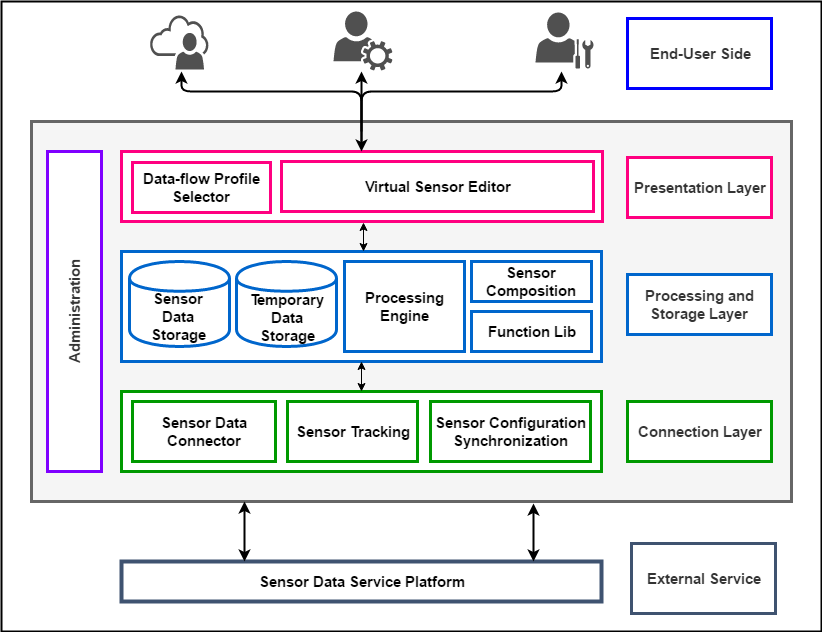
\includegraphics[width=0.72\textwidth]{./Part2/Chapter5/figures/vsf_architecture_overview.png} 
    \caption{The framework architecture overview}
     \label{fig:c5_vsf_architecture_overview}
  \end{center} 
\end{figure}

\subsection{Virtual Sensor Framework Workflow}
The overall blueprint of our sVSF workflow is shown in Fig.~\ref{fig:c5_vsf_operation_diagram} Physical sensors register their resource descriptions under CoRE Link Format~\cite{Shelby2012} with our backend. Once registered successfully, such sensors and resources are discovered through simple search queries. For instance, a query to search all the temperature sensor can be GET /rd-lookup/ep?rt=temperature. All sensing data from registered sensors will be forwarded to sVSF via SDSP. \\

In sVSF, VS function supports three types of the operator: rule, formula, and function. At the first state, the incoming data is received by connection layer. After that, this data is conveyed to Sensor Composition which handles and processes the VS operators and relationships in the logical data flow. This component also takes responsibility to convert VS operators to the proper mathematical operations and ensures it is executed in correct order in the processing engine. The conversions of VS operator into mathematical operation goes through two phases: First, the logical data flow content and sensor information are loaded into CP. More detail, as shown in Fig.~\ref{fig:c5_vsf_example}, a logical data flow comprises four VS operators, and sensor metadata are inserted in CP. Second, the particular variables of the operator are extracted and calculated by calling the corresponding functions in Function Lib Component (FL). These variables are reserved to simplify particular operations. For example, as shown in Fig.~\ref{fig:c5_vsf_example},  \$device.tank\_level\_change.data[24] represents all sensing data of “tank\_level\_change” sensor within 24 hours. After calculating, the values of special variables are added into virtual sensor operator before storing in temporary data storage in order to be reused in another stage. The lifetime of this temporary data can be set up by the sVSF administrators In the case of the virtual sensor has an input from another virtual sensor. This input value is also considered as a special variable and directly access via sensor name. For instance, sensor named “tank\_volume” can use the output value of “tank\_level” sensor via declaring a speacial variable named “tank\_level”. Furthermore, to maximize performance, Sensor Composition take responsibility for organizing the working schedule based on the asynchronous model. The un-relational virtual sensors, which are not linked together, will be arranged into the same thread and executed in parallel in processing engine. For example, in Fig.~\ref{fig:c5_vsf_editor_interface}, all green virtual sensors will be performed in parallel. \\

\begin{figure}[h!] 
 \begin{center} 
 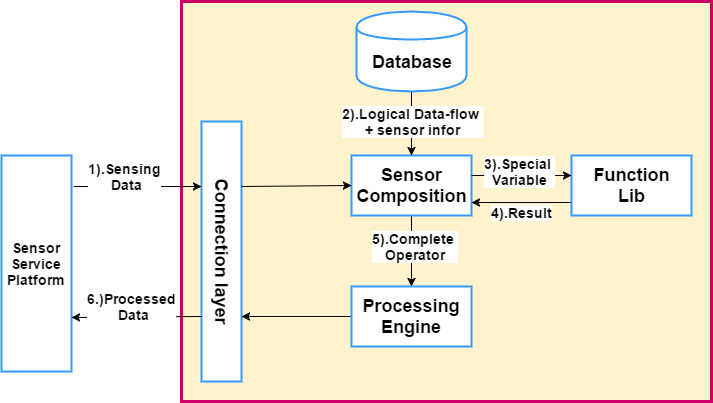
\includegraphics[width=0.82\textwidth]{./Part2/Chapter5/figures/vsf_operation_diagram.png} 
    \caption{The framework operation diagram}
     \label{fig:c5_vsf_operation_diagram}
  \end{center} 
\end{figure}

The most important component in processing layer is processing engine, where VS operators are executed. These executions are performed in parallel by a JavaScript library, namely MathJS . Finally, the output of processing engine will be stored in the database to be reused before responding final result to SDSP.

\section{Virtual Sensor Editor}
One of a key element of sVSF is an HTML5 web-based virtual sensor editor, which enables cross-platform development environment. The editor is a WYSIWYG (what you see is what you get) system. This allows the user to simply build a LDF by creating, configuring and connecting VSs together. VSE is implemented using native HTML5 and JointJS  library to maximize portability and availability across various end-user platforms. There are four highlighted attributes of this editor: (i) drag-drop interface: The end-user is able to simply create and link the virtual sensors by drag-drop action. (ii) Real-time Evaluation: After creating, user-defined LDF could be evaluated and receive result immediately. (iii) Reusability: VS configuration and LDF is stored and shared between the end-users. \\

\begin{figure}[h!] 
 \begin{center} 
 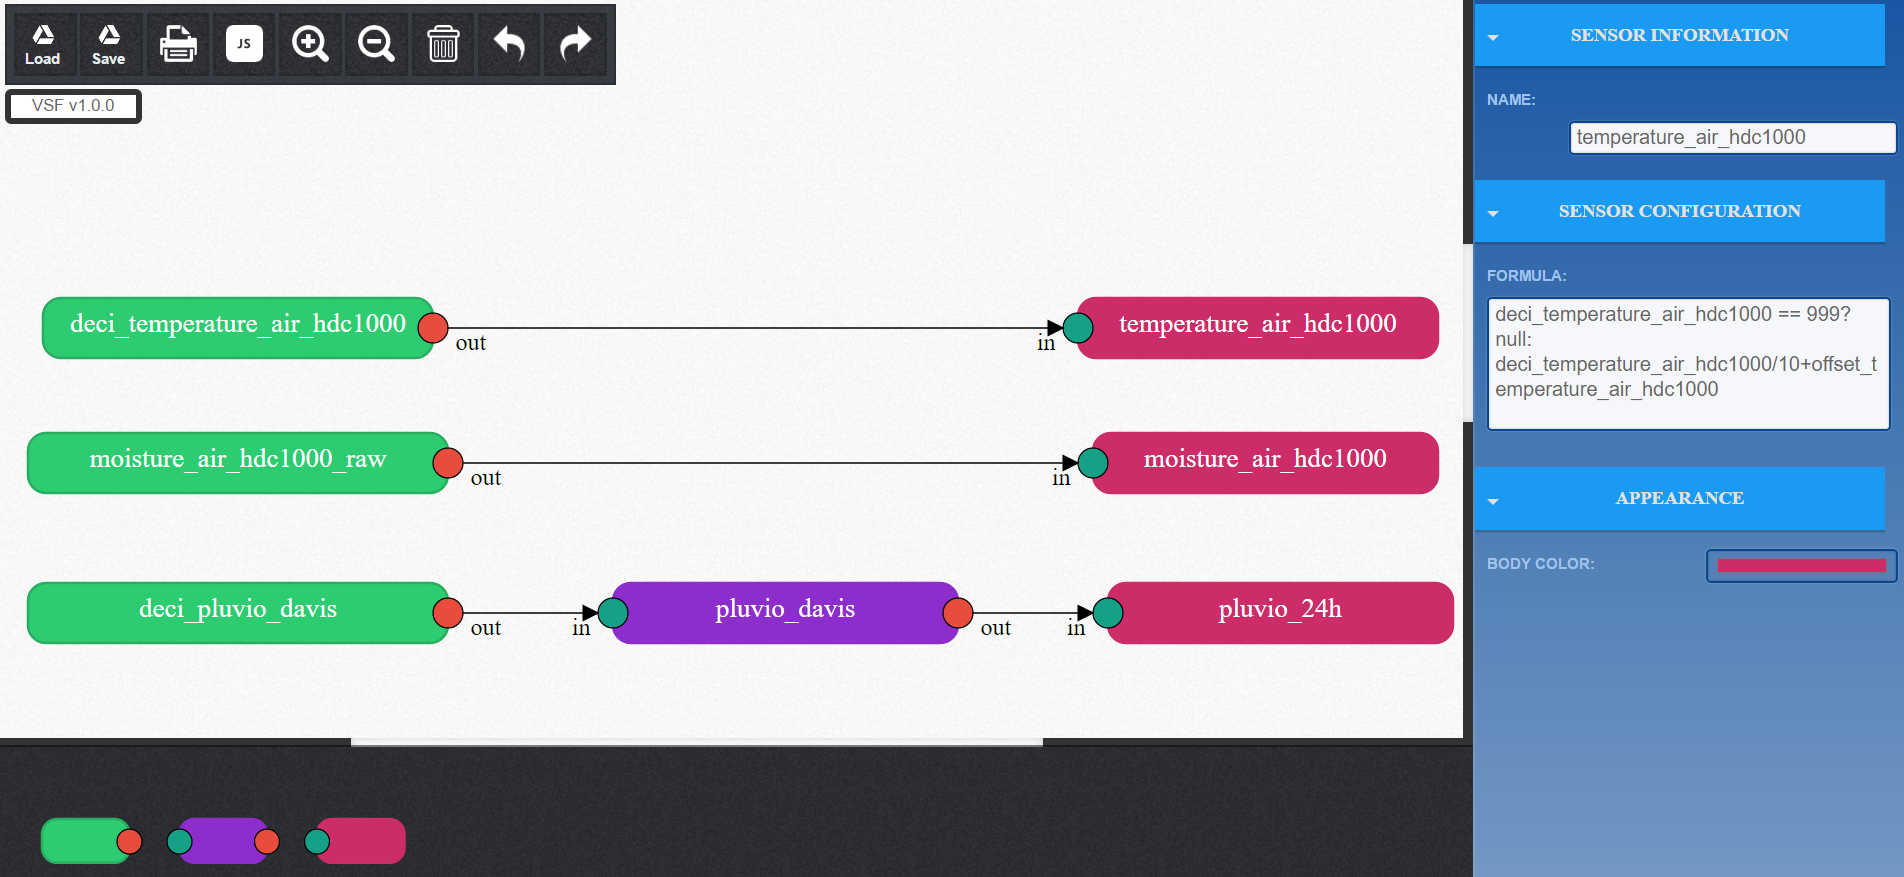
\includegraphics[width=\textwidth]{./Part2/Chapter5/figures/vsf_editor_interface.png} 
    \caption{Virtual Sensor Editor Interface}
     \label{fig:c5_vsf_editor_interface}
  \end{center} 
\end{figure}

As shown in Fig.~\ref{fig:c5_vsf_editor_interface}, a virtual sensor is represented as a box consisting of input, output ports and a VS operator. The number of these ports and sensor configuration depend on the type of virtual sensor. For example, a singular virtual sensor which serves as a physical sensor has one output and no input port. In Configuration panel on the left side, a drop box is added to allow the user to configure sensor driver. By default, we use the green and red color to identify virtual sensor type. But the end-user can change this attribute. Each output port can be assigned to one or more input of different boxes via data links. After data link is established, the later sensor enables to select the output of former sensor as an input parameter for its operator. The auto-complete feature is also equipped to speed up this selecting process. \\

Our sVSF offers recursive composing for the virtual sensor. A defined virtual sensor can be used as an input to construct other virtual sensors. After logical data flow is completely established, the evaluation feature enables the user to execute the data flow on self-generated data and receive the result immediately. Thus, the user can evaluate or correct the configuration in case of error. At the final state, the complete logical data flow is saved in the database and reused for next time.


\section{Evaluation}
In this section, we describe the utilization of our framework in a practical use-case. We also discuss how to archive high performance, scalability in our framework. Finally, an evaluation of our strategies is proposed.\\

\begin{figure}[h!] 
 \begin{center} 
 \includegraphics[width=0.95\textwidth]{./Part2/Chapter5/figures/vsf_example.png} 
    \caption{The generating high-level information process.}
     \label{fig:c5_vsf_example}
  \end{center} 
\end{figure}

Our first work has been applied to an industrial project for tank monitoring. The primary goal of this project is to manage the chemical volume via a level sensor which is plugged at the top of a tank.  The raw data of this sensor is the distance from the top of the tank to the chemical surface. Fig.~\ref{fig:c5_vsf_editor_interface} illustrates the whole process of generating high-level information such as remaining of the chemical level (Tank\_level), remains of chemical volume (Tank\_volume), change of chemical level (Tank\_level\_change), average on this change within 24h (Avg\_tank\_level\_change). Firstly, the raw data contains sensor information and sensed data is sent to sVSF. This data is handled by Sensor Composition where corresponding logical data-flow and sensor metadata is loaded from the database. In this case, the metadata is the tank information such as the height of tank (Tank\_high) and the total volume of tank (Tank\_total\_volume). At this component, special variables such as last value of such sensor (Tank\_leve.lastValue) or historical sensing data within 24h (Tank\_leve\_change.data[24]) are calculated by calling the corresponding functions in Function Lib component. All obtained information (special variable value, raw data value, sensor metadata) is injected into logical data low. Before transferring and executing at Processing Engine, logical data flow is converted to the mathematical operations. The final result is responded to SDSP via Connection Layer\\

\begin{figure}[h!] 
 \begin{center} 
 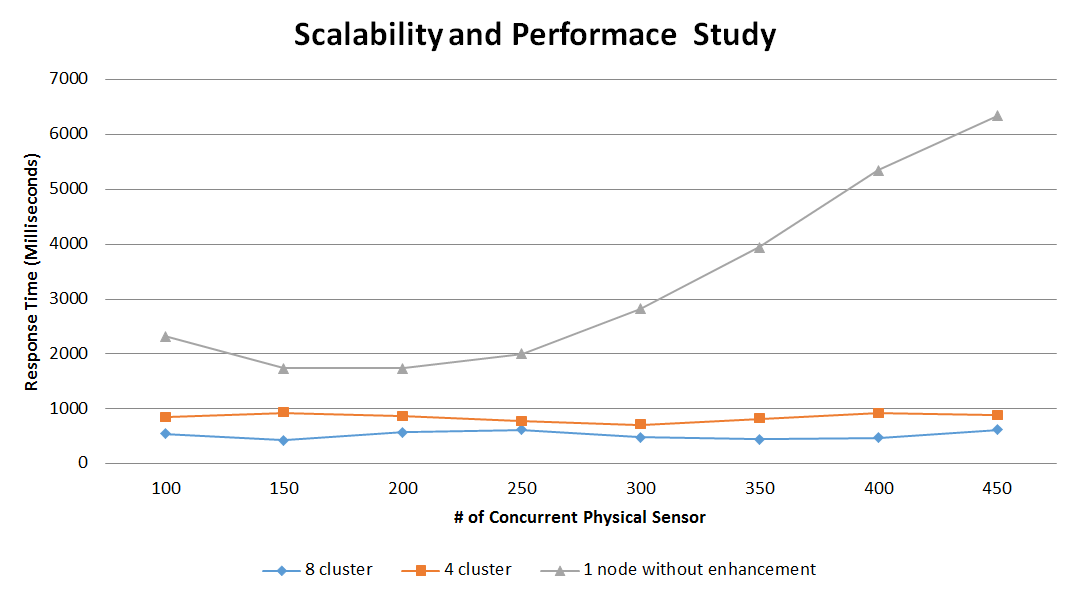
\includegraphics[width=0.8\textwidth]{./Part2/Chapter5/figures/vsf_scalability.png} 
    \caption{The effect of our enhancement in scalability and performance}
     \label{fig:c5_vsf_scalability}
  \end{center} 
\end{figure}

SVSF is developed by integrating MathJS library into NodeJS Express framework  which uses event-driven architecture. Nodejs also leverages a non-blocking I/O model that allows request being processed asynchronously. In order to enhance the framework scalability, we use clustering architecture. A cluster comprises a set of servers running simultaneously. Each server is called node. The cluster is elastic to adapt to the unexpected change in term of the number of concurrent user by dynamically add or remove a node to the cluster. There are two types of nodes: master node and worker node. The master node is used to manage the worker node in the cluster. It plays a role to distribute requests among different nodes in the cluster. Other strategies are proposed to increase the performance:

\begin{itemize}
    \item The first strategy is to store the output of the virtual sensor in a temporary database. Such value could be re-used as the input of other VS sensor instead of re-calculation.
    \item The second strategy is to use an in-memory database  to speed up data querying process. Our framework uses a NoSQL database named Apache CouchDB . Comparing with a relational database, CouchDB stores the data in an independent document and its self-contained schema. As the result, it provides a massive scalability and powerful full-text search
    \item The final strategy is to apply the asynchronous model to execute logical data-flow, meaning that all independent virtual sensor or virtual sensor in the same stage is executed in parallel.
\end{itemize}

To evaluate the effectiveness of proposed strategies, we have to consider two scenarios: (i) Significantly increasing the number of simultaneous physical sensor in SDSP. (ii) Increasing the complexity of logical data flow regarding the number of VS. All evaluations are performed on a computer with following configuration: Intel(R) Core(TM) i5-6200U CPU @ 2.30GHz, 2401 MHz, 2 Core(s), 4 Logical Processor(s), 8GB of RAM and the operating system is 64-bit Windows 10. The clustering model is set up and deployed using native Clustering Module  provided by NodeJS .The data rate of the physical sensor is one message per second. For the first scenario, we have conducted an experiment with different scale of sensor network, which increases from 100 to 450 concurrent physical sensors. The logical data flow comprises 50 virtual sensors. Fig.~\ref{fig:c5_vsf_performance} illustrates the performance changes after adopting our enhancements. As shown in the figure, our enhancement is remarkably effective. Without clustering model and enhancement strategies, the response time is significant increase when expanding the scale of sensor network. After applying clustering model using 4 or 8 clusters, the response time is highly stable under 1 second regardless the size of sensor network. With 450 concurrent physical sensors, the normal response time is over 6 seconds comparing with 875 milliseconds and 650 milliseconds of the model using 4 and 8 clusters respectively.\\

In the second scenario, the simulations are performed with different logical data flows size, which contains from 1 to 100 virtual sensors. Each logical data-flow is evaluated by various sensor network scale in SDSP. As shown in Fig.~\ref{fig:c5_vsf_scalability}, when increasing the number of concurrent physical sensor, the response time lightly increases regardless logical data flow size. In case the scale of the logical data flow is moderate (comprising under 50 virtual sensors), our system is able to serve a data message under 800ms even when 50 concurrent physical sensors are running. In the case of scaling up to 100 concurrent physical sensors, the response time is still under  1 second.

\begin{figure}[h!] 
 \begin{center} 
 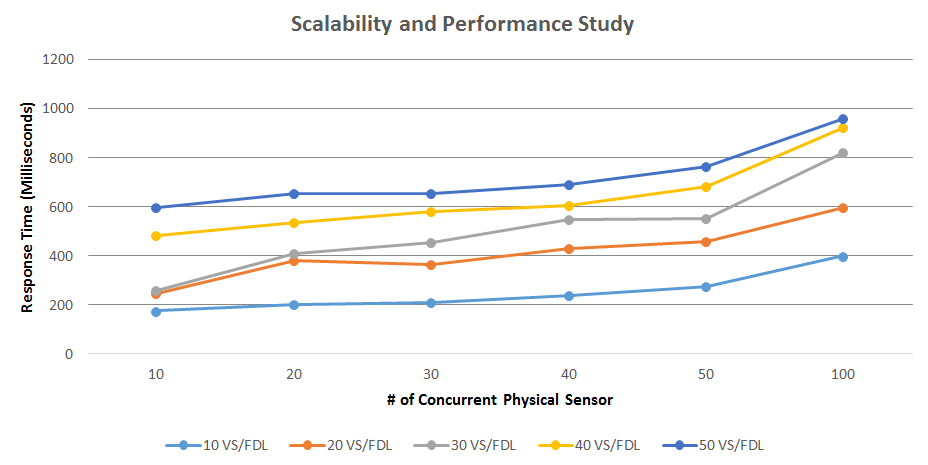
\includegraphics[width=0.8\textwidth]{./Part2/Chapter5/figures/vsf_performance.png} 
    \caption{The framework’s performance}
     \label{fig:c5_vsf_performance}
  \end{center} 
\end{figure}

\section{Conclusion}
In this chapter, we review a concept of the virtual sensor and propose a new virtual sensor taxonomy based on its functionality. The limitations of the existing virtual sensor frameworks are also considered in term of virtual sensor functionality and usability. Motivating to bridge the gaps, we proposed a scalable virtual sensor framework that allows producing high-level information from sensed data, by creating a logical data flow over a collection of the virtual sensor. A web-based virtual sensor editor is also offered to accelerate creating and configuring logical data-flow. In evaluation section, a serial of strategies to enhance the performance and scalability are discussed and evaluated. Regarding future works, we are currently working on integrating our platform into the oneM2M based framework~\cite{DattaGyrardBonnetBoudaoud2015} and FIWARE  architecture for ensuring interoperability.



\chapter{WoT-AD: A Descriptive Language for Group of Things in Massive IoT} 
\label{ch:Wot-AD}
\paragraph{}
Recently, the massive Internet of Things (Massive IoT) and Web of Things (WoT) are remarkable research fields aiming to facilitate the connectivity, accessibility and control of the Things by Web standards and technologies for large-scale deployment. In such context, the user is capable of simply creating, mashing-up and presenting the multiple Things to gain high-level information. However, current researches much more pay attention to describe a single Thing. The modeling and building the application for the compound objects consisting of groups of Things namely "Asset" are still limited due to the lack of description and seamless integration mechanism. 
Moreover, the traditional IoT Device Description Language directly installed on device is highly restricted in Massive IoT scenario because of stringent requirements for power consumption and operation cost.   
In this paper, we introduce the WoT based Asset Description (WoT-AD), a descriptive language for the Asset aiming to mitigate such limitations. WoT-AD explicitly describes a group of Things as homogeneous object to enable mash-up, self-discovery, and simply access their resources, entities, and services. We also provide a lightweight framework that fully integrates with WoT-AD to enable WoT for Massive IoT scenario. Such integration not only effectively models the Asset but also simplifies the development of mash-up application to different-skilled users. Finally, we evaluate the performance of our proposal to demonstrate its effectiveness and scalability in real use-case.
\section{Introduction}
Since the Internet inception in early 1980s, the Internet of Things (IoT) is considered as the first real evaluation of Internet \cite{lee2015internet} aiming to connect every object in the physical world into the digital world. With the exponential growth of the number of Things, IoT creates several business opportunities and estimates generating up to 11 trillion by 2025 \cite{manyika2015unlocking}. As a result, Massive IoT (MIoT)	is emerging	as a novel technology referring to huge volume of constrained IoT devices which stringently require excellent coverage, cost-effective and low-energy consumption. Among several new connectivity technologies for MIoT, proprietary LPWAN technologies such as Sigfox and LoRA have been considering the most potential candidates while cellular-based connectives such as 5G or NB-IoT are under developing and testing process \cite{raza2017low}. Although these protocols support collecting data from Things through the web protocols, the access and mash-up the Things resources are still limited due to lack of standardization and inter-operation. Thus, Things is usually formed into small and isolated silos for the application layers. \\

These considerations leverage to a novel concept named Web of Things (WoT) for directly collecting and accessing any Thing's resources as normal web resources. However, to fulfill Massive IoT requirements, there are some existing drawbacks mainly related to constraint in power and computing \cite{northstream_iot}. For example, we can not set up a high-level WoT application on the MIoT things, which is too costly to constrained devices. In the same situation, other effective solutions based on pub/sub model also suffer from the limit of LPWAN down-link. Most of them require the bi-directional connection to up-to-date the changes of Thing's resource while LPWAN connectivity only supports a limited down-link message per day \cite{sinha2017survey}. \\

At a higher level, the WoT is expected to break-down the Silo of Things by combining the traditional web paradigms with unified standards to present the things. This integration allows the Things to be published, managed and directly accessible as a normal web resource. To do so, logical interfaces of Things is used to present the information resources and services using Semantic Web languages and annotations such as the Device Description Language (DDL) \cite{chen2009device}, IoT-DDL \cite{khaled2018iot}, WoT-TD \cite{wc3_wot}, CoRE-TD \cite{7520965}. However, all of these approaches target to describe a single Thing that contains limited sensors and services. In reality, the Things may be a compound object including hierarchical group of thing and services. We named such things to be Asset. For example, in smart building scenario, the Asset could be a floor that including various rooms be monitored and controlled by IoT devices. Each room of this floor is considered as an independent Thing with different resources and services which are tightly linked to the devices. Therefore, we need a descriptive language to effectively describe either single or compound Things, that enhances the capability of access and managing the things. \\

In this paper, we propose an approach enabling the WoT for compound objects namely Asset in Massive IoT scenario. Our method is based on a novel semantic description (WoT-AD) and a light-weight WoT framework, which are fully integrated together for enabling WoT. Such combination is not only capable of presenting, accessing and managing the Asset but also speed up the development of applications for Massive IoT. 
According to our architecture, the Asset composing a group of things can be model as a uniform object that can be discovered, queried and visualized through an interactive interface. 
In addition, generating Asset description is facilitated to unskilled users via a graphic interface. This leads our propose adapting to a wide-range of Massive IoT use-cases. More in detail, our architecture composes of four primary layers as illustrated in Figure \ref{fig: Overview the Asset architecture}. The top of architecture is a composition layer that directly interacts with users. This layer supports composing the user's desire Asset from the available template. Then, the next layer named execution layer is used to (1) generate Asset API, (2) execute of Asses Model, (3) index the physical devices. The main component of this layer is virtual sensor framework which receives, processes and updates the Asset's resources from collected data. The last layer is connectivity layer which handles the connections from various IoT devices as well as external data sources (weather forecast, open IoT stream, e). The designed architecture is implemented as a framework following clustering model using Node.js language to enhance scalability and performance. We experimentally evaluate the framework in a Smart Space scenario. Finally, our contribution is highlighted following:
\begin{enumerate}
	\item Proposing the semantic description for the Asset named WoT-AD based on W3C things description \cite{W3C_TD}.
	\item Presenting a lightweight framework enabling WoT for Massive IoT scenario. Such framework fully exploits WoT-AD for composing, querying and managing the Asset through a uniform interface. The prototype is implemented following the clustering model along with various strategies to archive high scalability and performance.
	\item A cross-platform development tool on the top of the framework speed up the Asset development for non-tech-savvy user. 
\end{enumerate}

\section{Background analysis}


In this section, we briefly review the description of Things and current application for Web of Things. Their limitations are also identified. At the end of the section, we present our motivations to bridge the gaps by delivering a lightweight WoT framework along with novel description for group of things.
\subsection{Things Description}
To enable the IoT device integration into smart space, the Mobile and Pervasive Computing Lab at University of Florida presents the Device Description Language (DDL) based on the Service Oriented Architecture model. The IoT device in DDL is described as an entity including properties, internal mechanisms, and interfaces  \cite{chen2009device}. At first, the DDL is implemented and integrated within the Atlas sensor platform. Then, it is used to develop the Cloud-Edge-Beneath (CEB) architecture \cite{xu2016scalable} to handle Massive scale of sensors and devices in Smart city context. This CEB is based on Atlas architecture that allows end-user access directly to IoT devices or sensors through cloud interfaces \cite{bose2006building}\cite{chen2009atlas}. Atlas framework alone with DDL are implemented at Edge as an intermediate layer between cloud and "Beneath" layer. The author uses the Open Service Gateway Initiative (OSGi) to connect to Atlas sensor platform and discovery service. 

The World Wide Web Consortium (W3C) provides a WoT framework aiming to abstract the Things through a set of web services. To handle the digital presentation of the Things, W3C proposes the W3C Things Description (WoT-TD) consisting of (1) semantic description to present the general information of Things, (2) an interaction model with WoT properties, Action and Event to present the Thing's resources and services. (3) a semantic schema to express the data model \cite{W3C_TD}. The WoT-TD is used in \cite{kaebisch2016thing} to describe detail about how to control the different events and activities in specific domain.

To describe the Things in constrained environment, the Constrained RESTful environment (CoRE) based on Representation State Tranfer (REST) architecture is a common approach. CoRE applies Universal resource identifier (URI) to identify and discover the resources hosted by constrained nodes. The authors in \cite{7520965} replace CoRE link format by a semantic-based description named JSON-LD to enable seamless thing to thing interaction in the constrained environment.  A light-weight Things management framework residing in an M2M gateway is also proposed.
\begin{figure}[h]
	\centering
	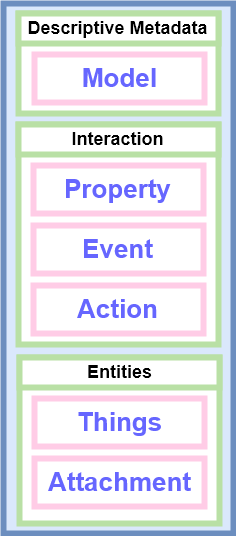
\includegraphics[width=8cm,height=12cm,keepaspectratio]{./Part2/Chapter6/figures/asset-descriptions-1.png}
	\caption{ : Overview Asset Model}
	\label{fig: Overview Asset Model}
\end{figure}
\subsection{Web of Things Framework}
Guinard \textit{et al.} propose a WoT framework that can generate a set of REST services to exploit and hierarchically link the sensor node resources via web interface\cite{guinard2009towards}. This speeds up creating ad-hoc applications for end-users. Their work is later applied in the AutoWoT project \cite{mayer2010facilitating} that aims to rapidly integrate IoT devices into WoT context by automatically building the web services to expose the device resources and functionality. AutoWot generates these web services based on a hierarchical service descriptions created by the end-user for the specific device. In addition, a graphical user interface is also proposed to facilitate creating description process for developers and tech-savvy users.

Another academic framework involving REST principle for integrating IoT devices into the Web is WebPlug \cite{ostermaier2010webplug}, a WoT framework including several functional blocks allows to represent and manage sensor data as the web resources. The users can compose their personal services based on physical objects. These services and resources accessibility is enhanced by Meta-URL that is proved to bring considerable benefits in temp of resource discovery and creating mash-up WoT applications. In the same approach, Christophe \textit{et al.} \cite{christophe2011web} proposes a framework for creating and handling IoT devices as virtual objects according to the event-based rule schema. The author in \cite{orestis2012towards} presents a service-oriented framework supporting multiple real-time services for  Wireless Sensor Networks (WSN) and smart objects via the Web such as storage, sharing, discovery. SemSense framework \cite{moraru2011exposing} aims to collect, process, equip with semantic meta-data and publish on the Web according the linked data standard. SPITFIRE \cite{pfisterer2011spitfire} targets to unlock the uni-modal closed systems in WoT by generating the semantic sensor description and an effective searching mechanism. After abstraction, the sensors and Things are integrated into Linked Open Data (LoD) cloud. This effort makes the collected data easily accessible on the Web and accelerates the development of WoT applications. With the convergence of academic and commercial worlds, several Web platforms are emerging with the aim to abstract the heterogeneity of the physical devices by REST web services. There are well-known framework such as Xively \cite{Doe:2009:Online}, ThingSpeak \cite{thinkspeak:Online}, and ThingWorx \cite{thingworx:Online}. These frameworks support accessing and visualizing the device data from cloud. Moreover, a RESTful API is offered for developer to build the custom application on the collected data.

In the light of this state-of-the-art, there are still missing the semantic description and a lightweight IoT architecture seamlessly presenting and managing the compound objects, which are monitored by multiple IoT devices.
\section{Contribution}
\subsection{WoT Asset Description}
WoT Asset Description is considered as the major part enabling Web of Things in our propose. Before describing in detail, we have to identify the required components inside such Asset. The Asset must be able to briefly introduce and discovery itself via self-description meta-data. The existing resources and interaction method are also effectively described to be fully accessible via Web. In addition, the devices along with their services belonging to the Assess must be presented and managed via defined actions. 
% is composed of the self-description meta-data, resources, entities and services. In general, the meta-data section presents the general information of the Asset in Web context. The existing resources and interaction method are described in next section named Interaction. The last section named Entities consisting of the information attached things and service of the Asset.

Based on the structure and requirements outlined above, we propose the WoT Asses Description (WoT-AD), a semantic description considering as an abstract entry point of a group of Things enabling the effective discovering, accessing and management process. WoT-AD is an extended concept of the W3c Things description (W3C-TD), which uses a JSON-LD schema to describe the single Things. The WoT-AD structure consists of three primary sections as illustrated in Figure \ref{fig: Overview Asset Model}: 
(1) The Descriptive meta-data describes the general Asset information. 
(2) The interaction model presents the Asset Resources (ARs) under the semantic scheme.
(3) The Entities express the Things and services constituted of Asset and their relations. More details of each element are described below:
\begin{itemize}
	\item \textbf{Descriptive Meta-data Section:} This section characterizes the Asset by presenting the unique identifier (URI) along with general information such as name, model, description, link... 
	\item \textbf{Interaction Section:} This section presents the available resources and services on the Asset and the interaction method. Each resource is considered as an interaction pattern which contains two separated parts are descriptive meta-data and interaction information.  
	\begin{enumerate}
		\item Descriptive meta-data holds the general information and configuration of resources such as type, description.
		\item Interaction information holds the information to connect to the resources such as connection address, method.
	\end{enumerate}
	The interaction pattern is divided into three types: Property, Event and Action to present several resources. The Figure \ref{fig: Overview the WoT-AD interaction} illustrates the interaction section of a simple WoT-AD that uses to abstract a building floor as an Asset. 
	\begin{enumerate}
		\item The Property is used to express the state of Asset that is collected or calculated from the attached Things. The property value is timely updated by a mathematical formula complying with Virtual Sensor Framework. The end-user can directly access or observe such value via interaction information that is defined via URI. As shown in the example, the temperature of the meeting room in the floor is declared as an Asset property and updated from the average of environment temperature collecting by device 1 and device 2. An HTTP access API is also provided to obtain the value.
		\item The Event presents the special situation detected by a set of specific conditions on Property. When the condition is satisfied, the corresponding actions are triggered. For example, in Figure \ref{fig: Overview the WoT-AD interaction}, we identify the overheating event with the condition that the value of temperature property is higher than 30 degree and trigger the turn on air conditioner action. 
		\item The Action presents the supported functions of the Asset which could be triggered by the event. The user could also directly access and control the actuator via available services belonging the Asset. In the presented example, the turning on air conditioner action is trigger by the overheating event and the command is directly sent to actuator of device 3. 
	\end{enumerate}
	\item \textbf{Entities and Attachment Section:} This section describes the entities belonging to the Asset. In our proposal, the entity may be a Things or service named attachment. Each Thing contains the descriptive meta-data and the address to interact with Things resources and services. The attachment could be the cloud-based services such as open data server, repository, device management server. Such attachments are treated as a Things which has meta-data and interactive address.
\end{itemize}
\begin{figure}[h]
	\centering
	\frame{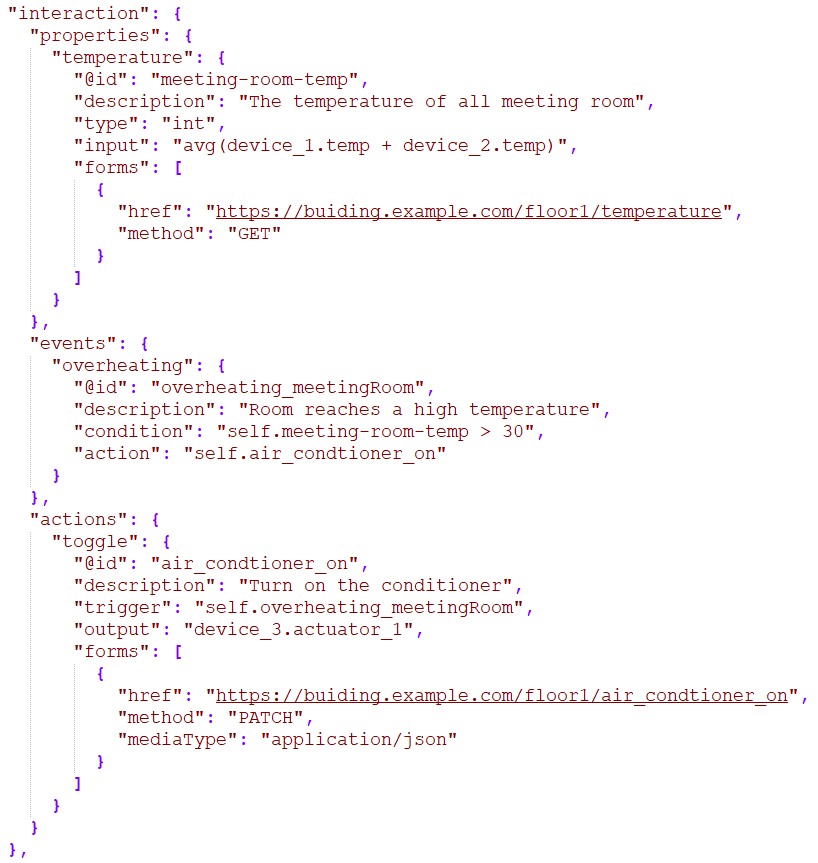
\includegraphics[width=0.9\textwidth]{./Part2/Chapter6/figures/wot-ad-2.PNG}}
	\caption{ : Overview the WoT-AD interaction section}
	\label{fig: Overview the WoT-AD interaction}
\end{figure}

\subsection{WoT Framework for WoT-AD}
\subsubsection{Principles and Design}
The overall goal of our proposal is to enable WoT for Asset in Massive IoT by providing a novel concept for Asset description along with an WoT framework. In addition, the framework facilitates the development of IoT applications on the Asset by providing a composition editor. For this reason, the designed architecture complies following principles:
\begin{itemize}
	\item High performance and low computational load for the server to adapt to Massive IoT scenario that must handle a large amount of connection.
	\item Effectively discovery, manage and access the Asset to fully aware of the real-world scenario. 
	\item Accelerating the development of IoT application on the Asset regardless of the user's skill.
	\item Handling the heterogeneity of constrained devices in LPWAN context. This enables the connection from a wide range of devices to framework effortlessly regardless of their characteristics. 
\end{itemize}
In order to archive these principles, we deal with several challenges listing below: 
\begin{itemize}
	\item The connectivity layer as the lowest part of architecture should be able to handle the connection from not only IoT devices but also the open data sources (open weather, open MQTT broker...). In addition, this layer needs to deal with the heterogeneity in term of LPWAN callback configurations. For example, the SIGFOX forwards the data via HTTP GET method whereas Lora Objenous uses HTTP POST method with different syntax. 
	\item The core of architecture must automatically discover and index the available resources in the Things which constitute of the Asset. These resources should be discovered in mash-up applications to facilitate the Asset creation procedure. This part also takes responsibility for real-time updating the Assess resources from collected data.
	\item The upper part of architecture must provide simple APIs to allow the user effectively discover, access and manage the Asset. A graphics editor is also provided to facilitate the Asset creation process.
\end{itemize}

\subsubsection{Overall Architecture}
\begin{figure}[h]
	\centering
	\frame{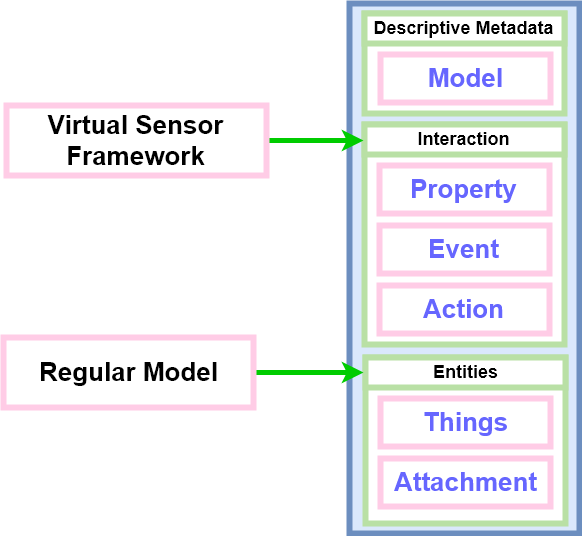
\includegraphics[width=12cm,height=16cm,keepaspectratio]{./Part2/Chapter6/figures/asset-operation-1.png}}
	\caption{ : Overview Operation Model}
	\label{fig: Overview Operation Model}
\end{figure}
Based on the listed principles and challenges, we propose a WoT framework fully exploit WoT-AD concept in Massive IoT scenario. The initial implementation of such architecture is represented by three main components spreading on horizontal layers, whose features properly fit the mentioned principles. The connector framework is used at lowest layer \cite{kim2017industrial} to handle the heterogeneous connections from both IoT devices and external data sources. The second component is the virtual sensor framework \cite{kim2017scalable}, an IoT framework supporting to create the logical data flow by visualizing the resources. The last component is a Graphic Editor facilitating the building and configuring process of the Asset by offering the drag-drop actions on HTML5 web interface. The overall of the framework is illustrated in Figure \ref{fig: Overview the Asset architecture}. The details of each layer are described below:
\begin{itemize}
	\item \textbf{Connection Layer:} This layer takes responsibility to handle the connection from LPWAN devices to the framework through dedicated connector. These connectors are simply created and managed by connector framework. At this layer, collected data from physical devices are aggregated and pre-process before conveying to upper layer. In case a new device connects to framework, the resources of this devices will be registered and tracked by sensor tracking services. 
	\item \textbf{Processing Layer} This layer is considered as a primary part of the architecture consisted of four main components: 
	(1) Virtual sensor platform is used to create the Asset by abstracting and linking the device resources together. This platform also has responsibility to update the Asset resources from collected data
	(2) Indexing: After successfully creating, the Asset resources are indexed by the indexing system. This guarantees all the resources are real-time discovered and synchronized with physical devices. 
	(3) Asset scripting is used to generate the Asset description and APIs based on defined resources. 
	(4) Asset model execution covert the Asset model to logical data flow \cite{kim2017scalable} be used by virtual sensor framework.
	\item \textbf{Presentation layer} This layer contains an interactive HTML 5 web interface, namely Asset Composer. This graphical interface provides the user several IoT components such as sensor, actuator, Asset, symbolic link. The end-user could simply create their own Asset by drag-drop actions. A dashboard to manage the existing Asset also proposed.
\end{itemize}
\begin{figure}[h]
	\centering
	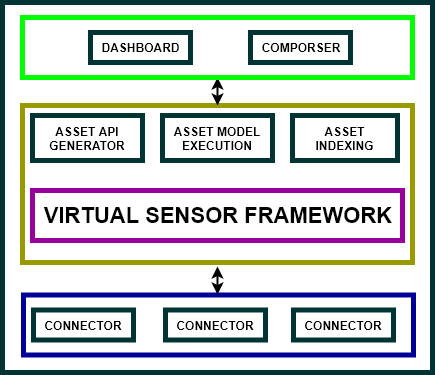
\includegraphics[width=0.9\textwidth]{./Part2/Chapter6/figures/overview_architecture.png}
	\caption{ : Overview the Asset architecture}
	\label{fig: Overview the Asset architecture}
\end{figure}
The primary requirement of WoT framework is that it must effectively and timely update and present the available resources. For this reason, we integrate our framework with a virtual sensor framework \cite{kim2017scalable} which provides self-discovery mechanism and supports generating the logical data flow from existing IoT devices. In general, an Asset is a self-operation object which is periodic updating its property values via an assigned logical data flow. The end-user can configure this frequency in Asset descriptive meta-data section.\\

The Asset's properties operate as a virtual sensor to retrieve and present the collected information from IoT sensors or devices. The elements in the Interaction section are build based on complex event processing (CEP) engine \cite{chen2014complex}. Therefore, if the current Asset properties reach a certain condition, the corresponding events are inferred and triggered the action. For example, we present the building floor as an Asset with the properties are the C02 and Humility of each room on the floor. If the CO2 degree of 75\% room is higher than 1000 ppm, the "suffocating" event is inferred and the system will send instruction command to relevant actuators to open window.


\section{Evaluate}
In order to validate the concept of WoT-AD and WoT architecture from the functional point of view, we have utilized the smart space scenario including a Raspberry Pi model B, which is considered as smart gateway be installed our WoT framework. In such context, the floors consisting of a set of rooms are considered as the Assets which are monitored by various IoT devices. Each device provides different resources and services. For example, the monitoring device equipped with multiple sensors including Co2, humility, PIR (motion detection), temperature, light. All collected information is used to control the air conditioning and light system for saving energy consumption. The control decisions are based on the whole floor status instead of the single room. Therefore, this context is the best practice to apply Asset. \\

Following the described scenario, a remote user can visually create and control an Asset via the interface of smart gateway. If the users use the existing Asset template, they only need to assign the IoT devices identification to the template. Based on this identification, these devices resources will be discovered and added to the interaction model of WoT-AD. Then, the complete WoT-AD is conveyed to processing layer where (1) Asset Script component creates the access API for the Asset resources, (2) Indexing component assigns a unique identity to the Asset for further self-discovery. Based on the composed Asset configure file, the logical-data flow is created to update the Asset properties from the collected information. This ensures the Asset data timely updated and reacted with the environment changes via configured events and actions in Asset's properties. \\

The software environment along with a light-weight local database for storing Asset configuration takes around to 100MB of spaces on the Raspberry Pi comparing with 32GB memory card. The most consumed operation of the framework is collecting, processing and updating the Asset information in processing layer. During the operational cycle mentioned in the scenario, the CPU load from 20 to 30 percent.
The high performance and scalability of such operation are ensured by Virtual Sensor Framework \cite{kim2017scalable}. 
\section{Results and discussion}
In a nutshell, this paper presents a semantic description for the physical Asset for enabling Web of Things in Massive IoT scenario. A WoT architecture is also defined and implemented to fully exploited the proposed concept. The architecture supports the interaction with various IoT devices and sensors based on the connector model implemented at lowest layer. The core element of the architecture is a framework named Virtual Sensor Framework that executes all the Logical data flow converted from Asset description. At the highest layer, we implemented a graphics editor fascinating the Asset description composing.\\
The effectiveness of designed solution was ensured by choosing and combining some technologies and IoT frameworks that have been practically demonstrated in real use-cases. To improve and extend the current works, we will optimize applied to smart building scenario. 
\section{Conclusion}



\chapter*{Conclusion of Part \ref{pa:part2}}
...... To be complete.............

\part{Enhance Data Quality}
\label{pa:part3}
\chapter*{Overview of Part \ref{pa:part3}}
............. To be compeleted ..............

%\clearpage
\chapter{An Active Learning Method for Errors and Events Detecion in Time Series} \label{ch:CABD}
\section{Introduction}

Anomaly detection is an important tasks in several domains such as intrusion detection systems, financial fraud detection, especially in Internet of Thing (IoT). It has been estimated that collected data could contain from 2.3\% to 26.9\% error rate~\cite{goldberg2008analysis}. Applications built upon imprecise time series can potentially result in losses in the millions of dollars to businesses~\cite{cleaningSource}. As a concrete example, in forest fire detection many sensors are deployed to monitor the concentration of carbon-monoxide and various organic compounds \cite{alkhatib2014review}. Potential problems are detected before occurring by combining collected data with the external weather information (e.g., wind speed, temperature, humidity). Imprecise detection coming from abnormal data could significantly decrease the system reliability and results for remedial works. The efficacy of such system need to be in collusion with anomaly detection algorithms \cite{mehrotra2017anomaly}.\\

\par Anomaly detection over time series is often applied to filter out dirty data. This means that the detected points are discarded as useless noises. Unfortunately, the eliminated data may contain notable events, also known as {\em change points}. These changes occur by accident (e.g., a fire in a forest) or because of human intervention (e.g., watering the tree). Preserving these events is essential to interpret the context. For example, to optimize the watering schedule, a city environment management company deploys the sensors to monitor the impact of watering on soil humility under the trees. However, a significant increase of soil humility due to water can be detected as anomaly and removed from the data~\cite{kang2013prevention}. Thus, the ability to explicitly distinguish between anomalies and events is needed.\\

\par The first plot from the top in Figure~\ref{fig: picture 1} visually presents this challenge in real ultrasonic sensor data that we obtained from an IoT solution company. The sensor is plugged on the top of a tank to monitor its liquid level (y axis) over time (x axis). As shown in the figure, some sudden changes appear, either in isolation (time index 100, 140) or as small groups (time index 230). These are likely the abnormal values, such as sensor errors, and should be fixed or removed from the data set. On the other hand, the data change generated by filling the tanks (time index 280) should be preserved.\\

\par The most common anomaly detection methods on time series use traditional statistical methods, e.g., neighbor-based \cite{chandola2009anomaly}\cite{Breunig:2000:LID:335191.335388}\cite{tang2001robust}\cite{kriegel2009loop}, ensembles \cite{skyline}\cite{Pevny2016} or probabilistic models \cite{burnaev2016conformalized}\cite{ahmad2017unsupervised}. They consider a data point as an abnormal if it significantly differs from historical observations. Unfortunately, change points also have this property in practice. The detection methods recognize such change points as anomaly. For state-of-the-art anomaly detection methods such as Numenta\cite{ahmad2017unsupervised}, KNN-CAD\cite{burnaev2016conformalized}, the presence of change points in times series significantly decrease the quality of detection. This often leads to skip other true anomalies. The basic idea of Numenta and KNN-CAD is to use a training set ($x_1, …., x_m$) from historical data to predict the value of $x_{m+1}$. Then, they compute a measure of prediction error. At final step, the use a probabilistic model to estimate the anomalous state. The presence of change point in the historical data will directly affect the prediction result by disordering the sequence in training set. If these algorithms predict an abnormal point as a change point. This point could be ignored because the prediction error is minor. As shown in Figure \ref{fig: picture 1}, Numenta algorithm ignores all collective anomalies. The KNN-CAD fails in all its detection.
In addition, the performance of such detection highly depends on parameter configuration data specific. Owing these limitations, the detection result is very poor (The f-score is under 20\%), as illustrated in both Figure \ref{fig: picture 1} in problem statement and empirical experiments in the evaluation section.\\

% \paolo{explain that only part of the data is in the figure}

\par Since completely automatic anomaly detection might not work well without discrimination between anomalies and change points. One approach is to use supervised learning method \cite{agrawal2015survey}\cite{gonbadi2015supervised}\cite{ma2016supervised}. However, labeled data is not available in general. This motivates our idea to exploit on interactive approach. The goal is to minimize the user involvement while guaranty quality over the results of the process. This is achieved by an  active learning method is exploited to obtain the truth from users. Our experiments show that labeling a very limited number of data points can significantly increase the detection quality. 
To reduce the number of interaction, we propose a non-parametric algorithm, which accurately detects both anomalies and change points based on the combination of a novel concept of neighborhood, namely {\em Inverse Nearest Neighbor} (INN) and unsupervised probabilistic classification. The philosophy of INN derives from observing objects in reality. Two objects have close-bond if they have a two way connection. Applying this concept to data object, object A and object B have strong relation if A is the neighbor of B and vice verse, B is the neighbor of A. More detail of INN is described in Section 2.4. Leveraging the advantages of INN, the type of a data point can be classified through evaluating as set of scores, that are calculated from INNs properties. The benefit of INN concept is also demonstrated in detecting collective anomalies. If a data point is identified as a abnormal points, its INNs is highly anomalous. Our algorithm will propagate the anomaly score to such INN to expose the whole anomaly pattern. The Figure \ref{fig: innvsknn} illustrates the difference of INN and K-Nearest Neighbor (KNN). When evaluating a data point belongs a collective anomaly, its INN will be the entirety of such anomaly while its KNN contains both anomalous and normal points. We discuss more detail about novelties of INN in section 2.4.\\

\begin{figure}[ht]
	\centering
	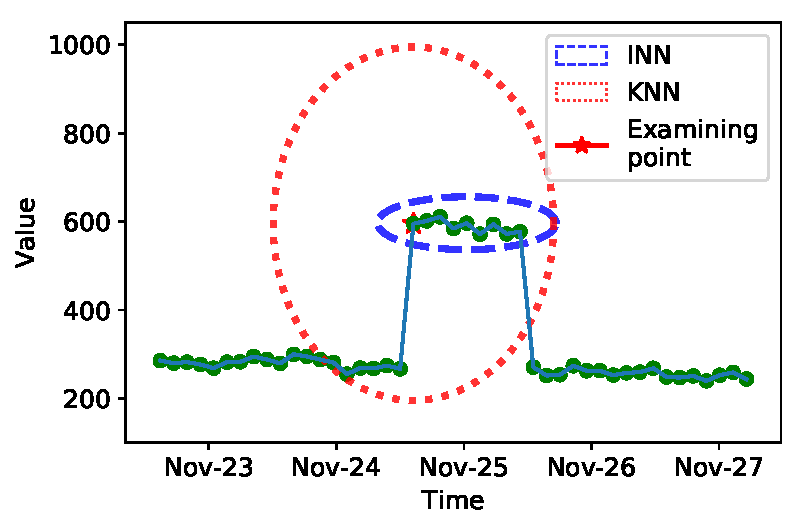
\includegraphics[width=0.8\textwidth]{Part3/Chapter7/figures/innvsknn.pdf}
	\caption{ : Compare Inverse Nearest Neighbor and K-Nearest Neighbor}
	\label{fig: innvsknn}
\end{figure}

\par Depending on the user-cases, user requires different detection quality. For example, fleet management application strongly requires high accuracy in discriminating the sensor errors and filling tank event while monitoring applications such as CO2 or temperature do not require such level of accuracy. This requirement leads to a new challenge how to satisfy user's desired quality why minimizing the user interaction? To address this challenge, the confidence of the classification model is used as termination condition for active learning process. More accuracy demands more points labeled to enrich the model until the classify confidence is achieved. Experiments demonstrate that with higher confidence requirement increases the F-score and it coverages to a consistent value.\\

\par Our method efficiently detects both anomalies and change points by taking advantages of Active Learning. We have implemented CABD as a python library. This prototype is empirically demonstrates producing high-quality detection in practical IoT user-cases. Our contributions in this work are summarized as follows:
\begin{itemize}
	\item CABD, a novel non-parametric algorithm for detecting both errors (i.e., single, collective anomaly) and events (i.e., breakpoints). 
	\item The novel concept of inverse nearest neighbor and active learning using uncertainty sampling scheme are applied to improve the CABD efficiency. 
	\item A prototype is implemented to evaluate CABD’s abilities in term of detection accuracy and response time in real IoT scenarios.
\end{itemize}
\par The remainder of this article is organized as follows. In Section 2, we formalize the problem of anomaly detection and related definitions. CABD is represented explicitly in Section 3. Section 4 evaluates quality of our method through two real use-cases. Section 6 discusses related works, and conclusion is presented in Section 7.  

\section{Preliminaries}
\subsection{Anomaly Types}

Anomaly detection is a technique used to identify unusual patterns that do not conform to expected behaviors, also called outliers. There are many applications in business, from intrusion detection to system monitoring. It is important to establish some boundaries on the definition of an anomaly. Anomalies can be broadly categorized as \cite{chandola2009anomaly}:
\begin{itemize}
	\item \textbf{Point anomalies}: A single instance of data is anomalous if it is significantly different from the remaining data.
	\item \textbf{Contextual anomalies:} The abnormality is context specific. This type of anomaly is common in time-series data. For example: 30 Celsius degree during summer is normal but may be abnormal in winter.
	\item \textbf{Collective anomalies:} This anomaly type contains a set of consecutive point anomalies to be represented as an abnormal data pattern. This pattern does not comply with the dataset distribution.
\end{itemize}

\subsection{Break Point}
In the simplest form, break point, also called change point, is the point at which the statistical properties of a sequence of observations change \cite{killick2014changepoint}. Break point detection is applied in vary application areas from finance, environment, health care to industrial maintenance~\cite{liu2013change}\cite{kawahara2009change}\cite{guralnik1999event}. More formally, let assume we have a time series $ X = \{x_1, x_2, ...., x_n\}$ which has $ m $ break points at the position $ \mathcal{C} = \{ c_1, c_2, ...., c_m \} $ with $ c_m < n $. The break points separate the data set into $ m + i $ segments such that the statistical properties of $ i^{th} $ segment $ \{ x_{c_{i-1}}, ... , x_{c_i} \} $ and $ (i+1)^{th} $ segment $ \{ x_{c_{i}}, ... , x_{c_{i+1}} \} $ are different in some way


\section{Problem Statement}
We consider a time series $ X = \{x_1, x_2, ...., x_n\}$ of $ n $ observations, where $ x_i $ is the $ i^{th} $ data point, may contain both errors and events. Its errors could be either single or collective anomalies and occur randomly. The main considerations are that, first, the event in X is usually detected as anomaly and simply discarded. Secondly, the detection performance is highly depends on configuration parameters which are data specific. Moreover, the present of change point also reduces such performance. Lastly, labeling anomaly data for training set requires immense manual labour. 
\par Let $ ac_i = \lbrace x_i, \ldots, x_{i+s} \mid x \in X, s \in \mathbb{N} \rbrace$, $as_i$ and $c_i$ denote a collective anomaly sized $ s $, single anomaly, change point at data point $x_i \in X$ respectively. The problem statements of our algorithm are formalized as follow:\\

\textbf{\textit{Problem:}} \textit{Given a desired detection quality and time series $ X = \{x_1, x_2, ...., x_n\}$, which has randomly abnormal points including both single and collective anomaly \\$ \mathcal{A} = \{ac_i, as_{t}, \ldots\}; $ $ i, t \leq n $ and a set of change points $ \mathcal{C} = \{ c_1, c_2, ...., c_m \} $ with $ m < n $. We aim to detect both $A$ and $C$ under a certain confidence level corresponding to the given quality while minimizing user interaction. 
}
\\
\par\textbf{Example 1} \textit{Consider time series X, a part of real IoT sensor data, has a collective anomaly occurring around Nov-24 and three single anomalies at Nov-10, Nov-14 and Nov-30 respectively. This time series also contains a change point about Dec-01. As shown in Figure~\ref{fig: picture 1}, all reviewed detection algorithms can not correctly detect the abnormality. For example, Numenta can not detect the sequence of errors and confuses change point with abnormal point. The detection result of KNN-CAD is even worth than Numenta. All single anomalies are mis-detected as collective anomalies. Our goals is to effectively detect both various kind of anomalies and change points in a single algorithm.}


\section{Inverse Nearest Neighbor}


\textbf{Definition 1}~(k-distance and nearest neighborhood of \textbf{p}): The k-distance of \textbf{p}, denoted as $ k_{dist}(p) $, is the distance $ d(p,o) $ between \textbf{p} and \textbf{o} in \textit{D}, such that for at least \textit{k} objects $ o' \in D/\{p\}  $ it holds that $ d(p,o') \leqslant d(p,o) $\\

\textbf{Definition 2}~(k-Nearest Neighborhood): The k-nearest neighborhood of p, denoted by $ NN_k(p) $ is the set of objects X in D with $ d(p,X) \leq k_{dist}(p) $.
\begin{equation}\label{key}
KNN_k(p)=\{ X \in D\/\{p\} | d(p,X) \leq k_{dist}(p) \}
\end{equation}

\textbf{Definition 3}~(Inverse Nearest Neighbor at k-distance): Given the time series $ X = \{x_1, x_2, .... , x_n\} $ and $x_i, x_j \in X$, if point $ x_i $ belongs to the nearest neighbor of point $ x_{j}$ at k-distance and vice versa, the point $ x_{j} $ belongs to the nearest neighbor of point $ x_{i} $ at k-distance, $ x_{j} $  is called as inverse neighbor of $ x_i $ at $k-distance $, denoted as:
\begin{equation}
\label{EQ: INN-definition}
 INN_k(x_i) = x_{j} \text{ \textit{iff} } 
 \begin{cases}
 x_i \in KNN_k(x_{j}) &     \\
 x_{j} \in KNN_k(x_i) & 
 \end{cases} 
\end{equation}

Inverse Nearest Neighbor at k-distance is the extended concept of Nearest Neighbor \cite{Huang2016} which lacks of checking reverse relation. The main purpose of INN is to identify the relation of two close data points. In reality,a data point and its INN may have the same characteristic. If this data point is anomalous, its INNs are highly anomalous which is in inverse proportion to their distance. That means the closer INNs have higher probability to be abnormal than others. The algorithm of finding INNs of a data point is described in Algorithm 1 that can automatically operate without any spacial parameters. In addition, we apply KD-tree~\cite{muja2009fast} to enhance searching performance.

\begin{table}[h]
	\centering
	\begin{tabular}{l}
		\toprule
		\textbf{Algorithm 1:} INN Searching of data point $ X_i $\\
		\midrule
		\textbf{Input: } kd-tree of time series X and data point $ X_i $ \\
		\textbf{Output:} List of INN's $ X_i $ \\
		1.~ Initializing: flag = 0, k = 1, $ INN(X_i) = \varnothing $	 \\
		2.~ Use kdtree to find the $ k $ nearest neighbors $ Y $ for $ X_i $ \\
		\hspace{10mm}$
		\left \|  
		\begin{tabular}{l}
		Find the $ k $ nearest neighbor for each $ Y_i \in Y $  \\
		\textbf{If} $ X_i \in KNN(Y_i)$ \textbf{and} $ Y_i \notin INN(X_i)  $ \textbf{then} \\
		\hspace{10mm} $ INN(X_i) = INN(X_i) \cup (Y_i,k) $  \\
		\end{tabular}
		\right .
		$\\
		3.~ Compute the size $ NNK(X_i) $\\
		\hspace{10mm} \textbf{If} this size does not changed \textbf{}\\
		\hspace{10mm} \hspace{10mm} \textbf{Return} $ NNK(X_i) $ \\
		\hspace{10mm} \textbf{Else}\\
		\hspace{10mm} \hspace{10mm} k++ \\
		\hspace{10mm} \hspace{10mm} go to step 2\\
		\hspace{10mm} \hspace{10mm}\\ 
	\end{tabular}
	\label{tab:INN_searching}
\end{table}
\begin{figure}[ht]
	\centering
	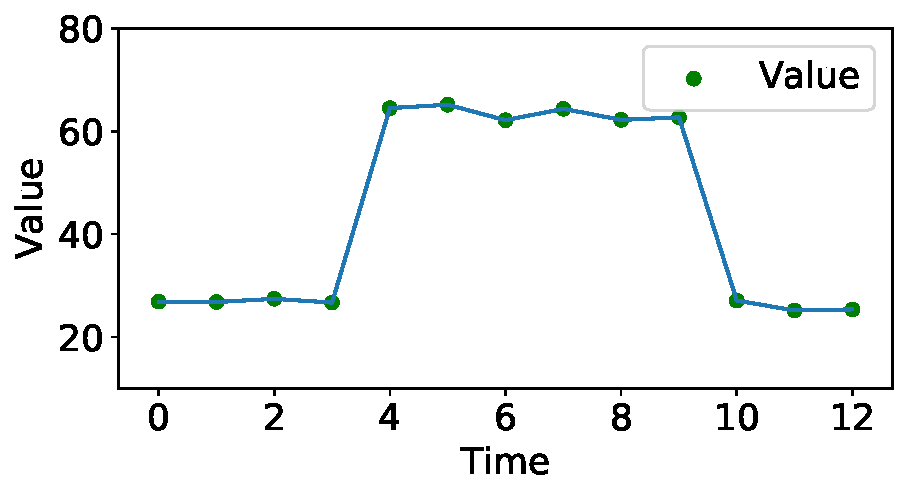
\includegraphics[width=0.8\textwidth]{Part3/Chapter7/figures/innvsknn_1.pdf}
	\caption{ : An Example of INN}
	\label{fig: innvsknn_1}
\end{figure}

\textbf{Example 2} \textit{\label{ex: 2} Consider the time series $X = $ \{26.87, 26.8, 27.42, 26.69, 64.51, 65.16, 62.15, 64.37, 62.21, 62.71, 27.07, 25.17, 25.364\} with thirteen data points in Figure~\ref{fig: innvsknn_1}, which contains collective anomaly on six points from $x_4$ to $x_9$. Assuming that we would like to find the INN of $x_4$. Let start at k = 1, we have $KNN_1(x_4) = \{x_5\}$ and $KNN_1(x_5) = \{x_4\}$. Referring to Equation~\ref{EQ: INN-definition}, $x_4$ and $x_5$ are INN at distance 1. Similarly, with k value from 2 to 5, we identify $\{x_6,\ldots,x_9\}$ belonging INN of $x_4$ \\
Let describe in detail at $k=6$, for simplicity, we use Euclidean Distance to calculate the distance between data points. With $
d(x_4, X) = $[37.86, 37.83, 37.14, 37.03, 0.0, 1.19, 3.09, 3.0, 4.61, 5.31, 37.93, 39.76, 39.96], we have $KNN_6(x_4) = \{x_5, \ldots, x_9, x_3\}$. Because of $\{x_5,\ldots,x_9\} \in INN(x_4)$, we will exam $x_3$. Using Euclidean Distance, we calculate $d(x_3, X) = $ [3.01, 2.0, 1.24, 0.0, 37.03, 38.52, 35.59, 37.89, 35.87, 36.52, 7.01, 8.14, 9.1]. Based on this distance we have $KNN_6(x_3) = \{x_0,x_1,x_2, x_{10}, x_{11}, x_{12}\}$. As we see, $x_3 \in KNN_6(x_4)$ but $x_4 \notin KNN_6(x_3)$. Therefore, $x_3$ does not belongs KNN of $x_4$. The INN searching for $x_4$ is stopped.}\\

\textbf{Definition 4}(Absolute first difference). The absolute value of first difference of $ x_{i} \in X $, denoted as $ \triangle x_i $, which is defined that:
\begin{equation}\label{First_difference}
\triangle x_i(p) = |x_{i}(p) - x_{i-1}(p)|,\, i = 1, 2, 3, ..., n
\end{equation}

\textbf{Definition 5}(Absolute Second difference). The absolute value of second difference of  $ x_{i}(p) $, denoted as $ \triangle '' x_i $, which is defined that:
\begin{equation}\label{Second_difference}
\triangle '' x_i(p) = |\triangle x_{i} - \triangle x_{i-1}|,\, i = 1, 2, 3, ..., n
\end{equation}

\textbf{Example 3} \textit{Consider again the time series in Example 2 $X = $ \{26.87, 26.8, 27.42, 26.69, 64.51, 65.16, 62.15, 64.37, 62.21, 62.71, 27.07, 25.17, 25.364 \}. Referring to Equation~\ref{First_difference}, the absolute first and second difference of $x_3$ are $\triangle x_3 = |x_3-x_2| = |27.42 - 26.8| = 0.62$ and $\triangle '' x_3 = |\triangle x_3 - \triangle x_2| = ||27.42 - 26.8| - |26.8 - 26.87| = 0.54|$}\\

\textbf{Definition 6}(Decay value). Decay value is the constant decrease in time. For example: $ x_i = 1 $, decay value = 0.2, so that $ x_{i+1} = x_i - decay \, value = 0.8 $

\section{Detection Algorithm using Active Learning}

Unlike the existing anomaly detections that only targets on detecting either single or collective anomaly and share common vulnerability to parameter configurations. We propose a comprehensive detection, being aware of both the anomaly and change point. In addition, applying Active Learning is not only significantly increase the accuracy but also reduce the sensitivity of (optimize) parameter configurations. In this section, we first present the overall algorithm. Then, we briefly explain each step along with related definitions.

\subsection{Overview algorithm}
Let $ X = \{x_1, x_2, ...., x_n \} $ denotes a time series, where Y and Z are set of anomaly points and break points of X respectively. Algorithm 2 presents the major steps of our proposal, which takes X as an input and produces Y and Z including their confident weights. Our algorithm also allows end-users to configure the desired confidence weight to ensure detection quality. The major steps are described as below:
\begin{enumerate}
	\item \textbf{Candidate Estimation}, in Line 1, generates the potential candidates, denoted by $ \theta $, from the extreme values in time series based on absolute second derivative.  
	\item \textbf{Score Computation}, in Line 3, computes score metric from INN of each candidate $ x_i $ in $ \theta $. This metric includes magnitude score, correlation score and variance score, denoted as $ \beta^{(x_i)} $
	\item \textbf{Score Evaluation}, in Line 4, uses a probabilistic classification to classify the candidates into three classes including change points, single anomaly points  or collective anomaly replied on the score metric. Active learning using the uncertainty model, described in equation \ref{equation:uncertainty_score}, is also applied. The most uncertain points will be queried and labeled to optimize the classifier. The output of this step is the confidence weight (CW) (denoted as $ \eth^{(x_i)} $) which is also known as anomaly score.
	\item \textbf{Anomaly Score Propagation}, propagates the anomaly score to its INNs in case the examining point is detected belonging to an anomaly pattern.
	\item \textbf{Classification Evaluation}, is the step to trigger the active learning process if the minimum of confidence weight is lower than user's quality requirement.

\end{enumerate}


\begin{table}[h]
	\centering
	\begin{tabular}{l}
		\toprule
		\textbf{Algorithm 2:} Anomaly and Change Point Detection\\
		\midrule
		\textbf{Input: } time series X, threshold $ \gamma $ (optional) \\
		\textbf{Output:} Error list $ Y $, change point list $ Z $ \\
		1.~ $ \theta \leftarrow $  Candidate(X) \\
		2.~ Y, Z = [ ] \\
		3.~ \textbf{For} $ x_i $ \textbf{in} $ \theta $ \textbf{do} \\
		\hspace{10mm}$
		%\left \|  
		\begin{tabular}{l}
		$ \beta^{(x_i)} \leftarrow $ Score($ x_i, X $) \\
		%$ \eth^{(x_i)} \leftarrow $ Evaluate($ \beta^{(x_i)} $)\\
		%$ UC^{(x_i)}, Y, Z \leftarrow $ Evaluate Detection($ \eth^{(x_i)} $)\\
		
		\end{tabular}
		%\right .
		$\\
		4.~  $ \eth^{} \leftarrow $ Evaluate($ \beta^{} $)\\
		5.~ $ CW^{}, Y, Z \leftarrow $ Evaluate Detection($ \eth^{} $)\\
		6.~  Y $\leftarrow$ Score Propagation($ \eth^{} $)\\
		7.~  \textbf{If} min(CW) $ \leq \gamma $  \textbf{then} \\
		\hspace{10mm}\textbf{Labeling} and \textbf{Go} to step 4 \\
		\\
		\hspace{5mm}\textbf{Return} $ Y, Z $\\
	\end{tabular}
\end{table}

\subsection{Anomaly Candidate Estimation}
Our goal is to intensively recognize both of errors and events. Therefore, we first introduce a method to identify the critical change in time series which also includes the detection of anomalous behavior. \\
Standard summary statistic such as mean, variance or correlation are common used in change detection. In our algorithm, we define the change of a point in time series based on its absolute second derivative. Formally, given time series X = {$ x_1, x_2,..., x_n $}. The change score of $ X $ is denoted by $ \partial $:
\begin{equation}\label{anomaly_score}
\partial(X) = \{\triangle"x_1, \triangle"x_2, ... ,\triangle"x_i\} | i \in \{1,2,...,n-1\}
\end{equation}
To identify the candidate, we use the statistically median absolute deviation (MAD) which is robust to anomalous data \cite{hochenbaum2017automatic}. If MAD of the change of a point is higher overall MAD standard deviation over the change of the whole data set, it is considered to be practically abnormal candidate. We will validate these candidates in the latter detection steps.\\
\par\textbf{Definition 17} Given time series X and the change score $ \partial $, MAD is defined as the median from sample median. 
\begin{equation}
MAD(X_i) = median(|\partial(X_i) - median(\partial(X))|)
\end{equation}

%Subsequently, we identify the peaks by using basic differentiation properties that the first derivative of a peak has a downward-going zero-crossing \footnote{\url{https://en.wikipedia.org/wiki/Zero_crossing}} at the peak maximum \cite{o1997pragmatic}. In the real-time series dataset, there are many false detections due to the noise. Therefore, the first derivate is smoothed before identifying downward-going zero-crossing. The extracted peaks are considered as the potential candidates for anomaly and change points. We will validate these candidates in the latter detection steps.\\
%\textit{Example:}....................\\

\subsection{Score Computation}

\par \textbf{Definition 7}(Spreading pattern) Spreading pattern (SP) of a data point is a set of data points from the examining point to its farthest INN. \\

\par \textbf{Definition 8}(Spreading size) Spreading size (SS) of a data point is the size of its SP. \\

\par \textbf{Definition 9}(Magnitude score) Magnitude score (MS) of data point is the radio of its Spreading Size over the size of dataset, denoted by MS. Given time series $ X = \{x_1, x_2, ..., x_n\} $ length $ n $ and $ x_i \in X $, the $ x_i $'s MS is defined as:
\begin{equation}\label{key}
MS(x_i) = \frac{SS(x_i)}{n}
\end{equation}

\par \textbf{Definition 10}(Piecewise Aggregate Approximation) Piecewise Aggregate Approximation (PAA) [*] transforms a time-series X of length n into vector $ \bar{X}=(\bar{x}_{1},.....,\bar{x}_{M}) $ with $ M \leq n $ where: \begin{equation}\label{PAA}
\bar{x}_{i} = \frac{M}{n} \sum_{j=n/M(i-1)+1}^{(n/M)i} x_{j}
\end{equation}

\par \textbf{Definition 11}(Symbolic Aggregate Approximation) Symbolic Aggregate Approximation (SAX) transforms a time-series X of length n into an arbitrary string by using PAA. A time series X length n can be represented by a word $ \hat{X} = \{\hat{x_1},\hat{x_2},....,\hat{x_n}\} $ with $ \hat{x_i} $ is a character of alphabet. Let denoted $ \alpha_j $ is the $ j^{th} $ element of the alphabet. $ \theta_{j-1} $, $ \theta_{j} $ are given thresholds.  
\begin{equation}\label{SAX}
\hat{x_i} = \alpha_j \,\,\,\,\,\, s.t \,\,\,\,\,\,\, \theta_{j-1} \leq PAA(x_i) \leq \theta_{j}
\end{equation}

\par \textbf{Definition 12}(Correlation Score) Correlation Score (CS) of a data point is the frequency of its Spreading pattern, which is represented as a string by using PAX. Given time series $ X = \{x_1,x_2,....,x_n\} $ and $ x_i \in X $
\begin{equation}\label{key}
CS(x_i) = frequency\left(\frac{SAX(SP(x_i)}{SAX(X)}\right) 
\end{equation}

\par \textbf{Definition 13}(Spreading pattern with k-neighbors) Spreading pattern with k-neighbors (SPk) of a data point is a set of data points from the point to its farthest INN including k adjacent points in both sides.\\

\par \textbf{Definition 14}(Variance Score) Variance Score (VS) describes the change of standard deviation of spreading pattern with k-neighbors after remove spreading pattern.
\begin{equation}\label{Variance Score}
VS(x_i) = \frac{std(X - INN(x_i))}{std(X)}
\end{equation}

As we discussed in previous section, the properties of a data point and its INNs are quite similar. Thus, we probably identify both point anomalies and collective anomalies through verifying its spreading pattern.
In this step, we compute the score metric of each candidate from step 1. There are three scores in this metric: (1) Magnitude score, (2) Correlation Score, (3) Variance Score. The detail of each score is clearly described in preliminary. In more detail, these scores are specifically represent the property of examining point. For example, magnitude score describes the proportion of spreading pattern of examining point in the dataset. Based on the anomaly definition, the size of anomaly  must be less five percent of dataset. Therefore, if the magnitude score is higher than five percent, the candidate probably is not an anomaly point. Similarly, correlation score represents the regularity of spreading pattern. \\

%Through these scores, we probably identify whether the candidates are abnormal points or change points. 
The algorithm 3 illustrates the score metric calculation process. We first find the farthest INN of examining point by using binary search which reduces significantly the complexity from $ n $ to $ log_2^n $. Next step, the scores are calculated in parallel to optimize performance. Finally, all score are collected and formed as a metric. 
\begin{table}[h]
	\centering
	\label{al-2}
	\begin{tabular}{l}
		\toprule
		\textbf{Algorithm 3:} Score Computation\\
		\midrule
		\textbf{Input: } Data point $ x_i $, time series X \\
		\textbf{Output:} Score Metric $ \beta^{(x_i)} $\\
		1.~ $ \eta \leftarrow $  SS($ x_i $, $ X $) \\
		2.~ $ \kappa \leftarrow $  MS($ x_i $, $ \eta $) \\
		3.~ $ \xi \leftarrow $  CS($ x_i $, $ \eta $) \\
		4.~ $ \varphi \leftarrow $  VS($ x_i $, $ \eta $) \\
		5.~ $ \beta^{(x_i)} \leftarrow $ [$ \kappa $, $ \xi $, $ \varphi $]  \\
		\textbf{Return} $ \beta^{(x_i)} $
		
	\end{tabular}
\end{table}

\subsection{Score Evaluation}

Replied on calculated metric scores, the Score Evaluation step uses a probabilistic classification algorithm to estimate the probability of data point $ x_i $ to be an anomaly point, change point or belonging to an anomaly pattern. CABD is designed with high modularity and flexibility. It allows to rapidly plug-play the classification algorithm depending on the context. By default, CABD use the random forest classification \cite{liaw2002classification}. Because of the variety of IoT scenario, obtaining a training set requires immense manual labour. Thus, without user intervention, the classification works on a set of initiated hypothesis. With the presence of human, the existing active learning using uncertainty sampling scheme \cite{cohn1994improving}, named CAL, is directly applied to increase classification performance by effectively labeling the most uncertain instances.\\ %The querying in CAL is made from the uncertainty of classification. \\

In CAL, we examine the most likely class of data points $ x_i \in X $ based upon the probability be done by classification algorithm. This probability is also considered as confidence weight of data instance. Then we decide whether or not to require its label $ y_i \in Y= $ \{abnormal point, anomaly pattern, change point\}  from human labeling process replied on the uncertainty of classification defined by:
\begin{equation}\label{equation:uncertainty_score}
\mathcal{U}(x) = 1 - P(\hat{x}|x)
\end{equation}
where $ x $ is the data point and $ \hat{x} $ is the most likely classification. The querying process of CAL is stopped if all confident weights are higher than a pre-configured threshold. By default, this threshold equals 0.8\\

\begin{figure}[h]
	\centering
	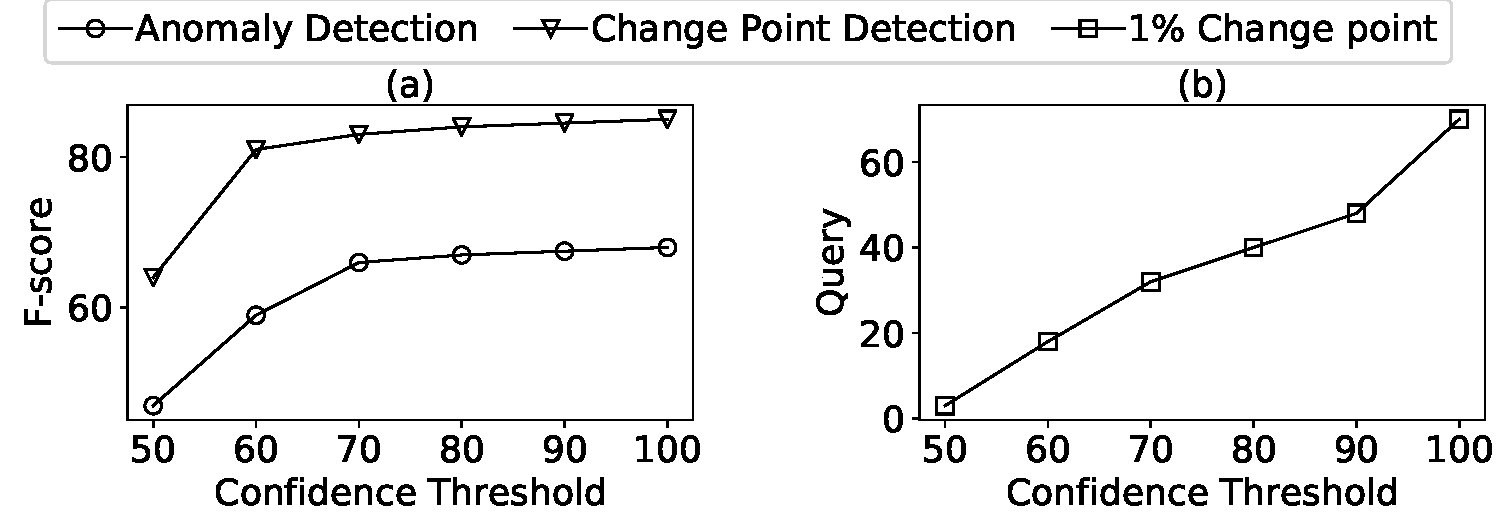
\includegraphics[width=\textwidth]{Part3/Chapter7/figures/new_compare_confidence.pdf}
	\caption{ : Varying confidence settings (a) Anomaly and Change point detection Accuracy, (b) The number of query}
	\label{fig:compare}
\end{figure}
\\
\textbf{Example } If data point $ x_i $ has classification possibility $ [0.1, 0.3, 0.6] $ to labels [abnormal point, anomaly pattern, change point], this point is the most likely change point with 0.6 confidence weight and $ 0.4 $ uncertainty. \\

The initial training set of the probabilistic classifier is build base on a set of hypothesis  $ \mathcal{H} $ which are include three main decision rules relied on score metric:

\begin{enumerate}
	\item The magnitude score (MS) of an abnormal point must be lower than $ k\% $. This means, the spreading pattern size of this point is lower than $ k\% $ of data size. Particularly, the spreading pattern size of single anomaly equals 1. 
	\item The correlation score of an abnormal point must be lower than $ c\% $. This means, the spreading pattern of this point must occur lower that $ c\% $ frequently in dataset
	\item The variance score of an abnormal point must be higher than $ v\% $. This means, the standard deviation of spreading pattern with k-neighbors must reduce at least $ v\% $ after removing the spreading pattern.
\end{enumerate}

From observing the properties of change point and various anomaly type in the practical dataset, we derive the set of threshold $ [k,c,v] $ is 0.05, 0.1 and 0.5 respectively. Given the set of examining data points X, label Y = \{abnormal point, collective anomaly, change point\}, threshold $ \theta =  [0.05, 0.1, 0.5]$, set hypotheses $ \mathcal{H} $ defined by:

\begin{equation}\label{hypothesis}
\left \{\begin{tabular}{c}
$ h_1 $ \, : \, \textbf{Anomaly Point} \quad \textrm{if} \quad $ \begin{tabular}{|l}
$ SS(x_1) = 1  $ \\
$ \beta^{x_i}_{\xi} \leq 0.1  $ \\
$ \beta^{x_i}_{\varphi} \geq 0.5  $ 
\end{tabular} $\\\\
$ h_2 $ \, : \, \textbf{Anomaly Pattern} \quad \textrm{if} \quad $ \begin{tabular}{|l}
$ \beta^{x_i}_{\kappa} \leq 0.05  $ \\
$ \beta^{x_i}_{\xi} \leq 0.1  $ \\
$ \beta^{x_i}_{\varphi} \geq 0.5  $ 
\end{tabular} $\\\\
$ h_3 $ \, : \, \textbf{Break Point} \quad \textrm{if} \quad $ \begin{tabular}{|l}
$ \beta^{x_i}_{\kappa} > 0.05  $ \\
$ \beta^{x_i}_{\xi} > 0.1  $ \\
$ \beta^{x_i}_{\varphi} < 0.5  $ 
\end{tabular} $\\
\end{tabular}
\right \}
\end{equation}


The algorithm 3 summaries the CAL for active learning in Score evaluation step. Let denote the $ \kappa $ and $ \varphi $ be the confident weight and uncertainty of data points respectively.

\begin{table}[h]
	\centering
	\label{tab:table2}
	\begin{tabular}{l}
		\toprule
		\textbf{Algorithm 3:} Score Evaluation\\
		\midrule
		\textbf{Input: } Unlabeled data set $ X $, probabilistic model $ Z $, \\ initial training set $ \mathcal{V} $, threshold $ \gamma $.\\
		\textbf{Output: } $ [\kappa $, $ \varphi $] \\
		1.~ [$ \kappa $, $ \varphi $] = Z(X,$ \mathcal{V} $) \\
		2.~ \textbf{While} $min(\kappa) \leq \gamma$ \textbf{do} \\
		\hspace{10mm}$
		\left \|  
		\begin{tabular}{l}
		$ x_t \leftarrow $ \textit{Query}($ x_t, \varphi ,X $) \\
		\textit{Label} $y_t$ for $x_t$\\
		\textit{Set} $ \mathcal{V} = \mathcal{V} \cup \{(x_t, y_t)\} $\\
		\textit{Update} $ [\kappa $, $ \varphi $] = Z(X,$ \mathcal{V} $)
		\end{tabular}
		\right .
		$\\
		
		
		\textbf{Return} $ [\kappa $, $ \varphi $]
		
	\end{tabular}
\end{table}

\subsection{Score Propagation}
The score propagation step selects the collective anomaly from the classification result and propagates the anomaly score to its INNs. The propagation step is control by decay values and the k-distance, this means the anomaly score of INNs near abnormal point to be more increased than others. By default, decay value of an data point equals the ratio of its anomaly score over its spreading size. Formally, given time series X, for each point $ x_i \in X $, $ \theta_{y_i} \in SP(x_i) $ is given by:
\begin{equation}\label{probagation_score}
\theta_{y_i} = \theta_{y_i} + \left( \theta_{x_i} - \alpha*k \right) 
\end{equation}
where $ \alpha = \frac{\theta_{x_i}}{SS(x_i)}$ and k are decay value and k-distance from $ x_i $ to $ y_i $ respectively. \\
\textbf{Example } Consider $ x_i $ has the anomaly score $ \theta_{x_i} = 0.8 $ and spreading pattern $ SP(x_i) = \left\lbrace [x_{i+1}, 1],[x_{i+2}, 2],[x_{i+3}, 3],[x_{i+4}, 4]\right\rbrace  $. The decay value of $ x_i $ is $ \alpha = \frac{0.8}{4} = 0.2$. Let assume $ \theta_{x_{i+3}} = 0.3 $, referring to Equation \ref{probagation_score}, we have anomaly score of $ x_{i+3} $ after propagating is:
\begin{equation*}
	\theta_{x_{i+3}} = 0.3 + \left( 0.8 - 0.2*3 \right) = 0.5 
\end{equation*}

\subsection{Complexity Optimization}
Among the major step in Algorithm, the Score calculation step is optimizable in searching INN of candidates. First, we identity that INN searching cost could be pruned by applying the binary search method which reduce the searching complexity from O(n) to O(Log n). Moreover, we add a new the stopping condition of INN searching based on maximum size of INN. \\

\textit{Intuition}: Recall that when searching the INN of data point x denoted INN(x) in Algorithm 1, the k value denoted the size if INN(x) starts at one and increases by one until k is not change. The complexity of such approach is O(k) with k is the size of INN(x). This could be optimized by using binary searching method to find the INN set for both side of examining point. The complete INN is the union of these sets. The complexity will be reduced from O(n) to 2*O(Log n). The operation of binary search requires maximum searching positions as an mandatory input. In practice, if the size of an abnormal pattern is higher than five percentage of data set, it could not be considered as collective anomaly. Thus this boundary is used as the maximum searching range.\\

Given data point $x_i$, searching range threshold $t$. The algorithm 4 illustrates the Binary INN searching for the right side of data point $x_i$
 
\begin{table}[h]
	\centering
	\begin{tabular}{l}
		\toprule
		\textbf{Algorithm 4:} Binary INN searching\\
		\midrule
		\textbf{Input: } Data point $x_i$, threshold t \\
		\textbf{Output:}  $INN_R(x_i)$\\
		1.~ $ L = i; R = t - 1; INN_R(x_i) = [ ]; $\\
		2.~ \textbf{While} $ L \leq R $ \textbf{do} \\
		\hspace{10mm}$
		\left \|  
		\begin{tabular}{l}
		$m = floor((L+R)/2)$ \\
		\textbf{If} $x_m \in KNN(x_i)$ \textbf{and} $x_i \in KNN(x_m)$\\
		\hspace{5mm}$ L = m + 1$\\
		\textbf{Else}\\
		\hspace{5mm}$ R = m - 1$\\
		
		\end{tabular}
		\right .
		$\\
		4.~  $INN_R(x_i) = [x_i, \ldots, x_m]$\\
		5.~  \textbf{Return} $ INN_R(x_i) $
	\end{tabular}
\end{table}


\section{Evaluation}


In this section, we experimentally evaluate the quality and efficiency of our proposal on both real and synthetic datasets. Such results are also compared with one of common anomaly detection approaches. Our goal is to demonstrate that:
\begin{itemize}
    \item The superiority of CABD in both detection quality (anomaly, change point detection) and runtime over real and synthetic datasets. 
    \item The effectiveness of INN concept and active learning in our propose.
    \item CABD could be a complementary part to enhance data repairing algorithms.
\end{itemize}


%In this section, we empirically evaluate the quality and efficiency of our proposal on both real and synthetic dataset. We demonstrate that:
%\begin{itemize}
%	\item CABD effectively detect both single and collective anomalies which need to be removed.
%	\item CABD quickly identify the key deviation event which also known as break point.  
%	\item Applying active learning significantly improves the CABD’s accuracy. 
%\end{itemize}
%We briefly describe each of these goals below

%\subsection{User studies}
%\subsubsection{User study 1: Tank Monitoring}
%\subsubsection{User study 2: Humility Monitoring}


\subsection{Metric of measurement}
For evaluating the efficiency of proposed algorithm, we use three common metrics named Precision, Recall and F-score. .Let S be the number of the outliers or change points detected by the algorithm and G be their ground truth. The precision (P) and recall (R) are defined as
\begin{equation}\label{Precision}
Presicion = \frac{|{S}|\cap{G}}{|{S}|}
\end{equation}
and
\begin{equation}\label{Recall}
Recall = \frac{|{S}|\cap{G}}{|{G}|}
\end{equation}
respectively. F-score or F-measure, a simple way to balance the P and R of an overall detection result, is defined as: 
\begin{equation}\label{F-score}
F\-score = 2 * \frac{P * R}{P + G}
\end{equation}

To assess the advantage of using interactive learning in comparison to manual update of all cases, we use a benefit function calculated from the cost ratio as the number of actions divided by the number of errors \cite{he2016interactive}. Formally, given the number of query by active learning $ T_A $ and manually update $ M $, we defined the benefit of the algorithm as: 

\begin{equation}\label{func: benefit_function}
BNF = 1 - \frac{T_A}{M}
\end{equation}

\subsection{Benchmark dataset}
\subsubsection{Real dataset}

\begin{figure*}[h]
	\centering
	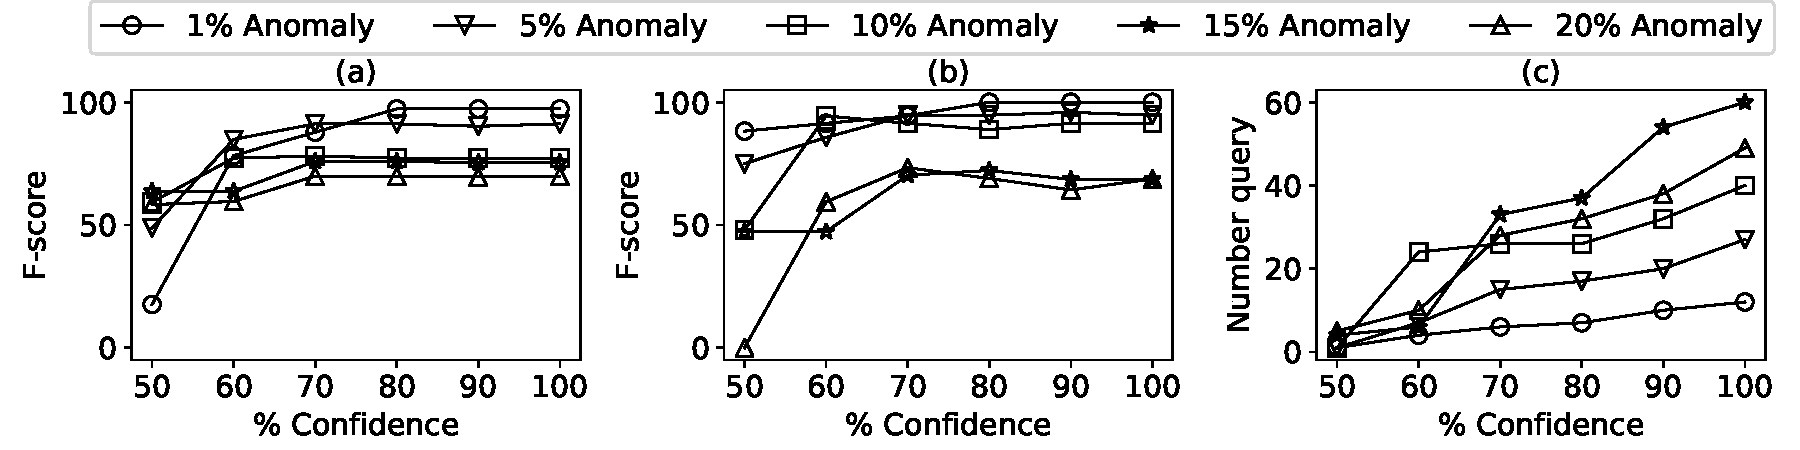
\includegraphics[width=\textwidth,height=\textheight,keepaspectratio]{Part3/Chapter7/figures/new_changeALpercentage_with1CP.pdf}
	\caption{ : Evaluation on varying Confidence Weight. From left to right, the three plots show: (a) Anomaly detection quality, (b) Change point detection quality, (c) The number of query to achieve given Confidence Weight}
	\label{fig: confident_1CP_compare}
\end{figure*}

\textit{IoT data with real errors:} The data is collected from 2 real ultrasonic sensors deployed on the top of tanks. Errors naturally occur without any human interactions ($ https://github.com/kimhungGCZ/anomaly\_dataset $) . Since we entirely manage the tank operations such as filling or consuming, the errors and change points are manually labeled as ground truth. \\

\textit{Yahoo data with real error:} The yahoo lab data ($ http://labs.yahoo.com/Academic\_Relations $) provides a number of datasets taken from real production traffic to some of Yahoo's properties. The abnormal points of such datasets are marked by humans so they are probably not consistent. In addition, the change points are not presented. Therefore, the datasets are best used to measure the recall factor of anomaly detection.

\subsubsection{Synthetic dataset}
Synthetic datasets aim to assess the efficacy of our algorithm in the presence of various anomaly types (local, global, single, collective anomalies) and change points in different proportion. To create these datasets, we first generate the data points following real data distribution. Then we fit this curve to a time series obtained from IoT production environment to preserve the trend and seasonality. Lastly, we randomly inject a mix of anomaly types with varying widths and magnitudes. These anomalies also recorded to evaluate against the points detected by our proposed algorithm. Figure \ref{fig: data_1_ex} illustrates a part of synthetic dataset named \textit{ds-1} that includes global, local and collective anomalies. Two notable events are also reported as the change points. 

\begin{figure}[H]
	\centering
	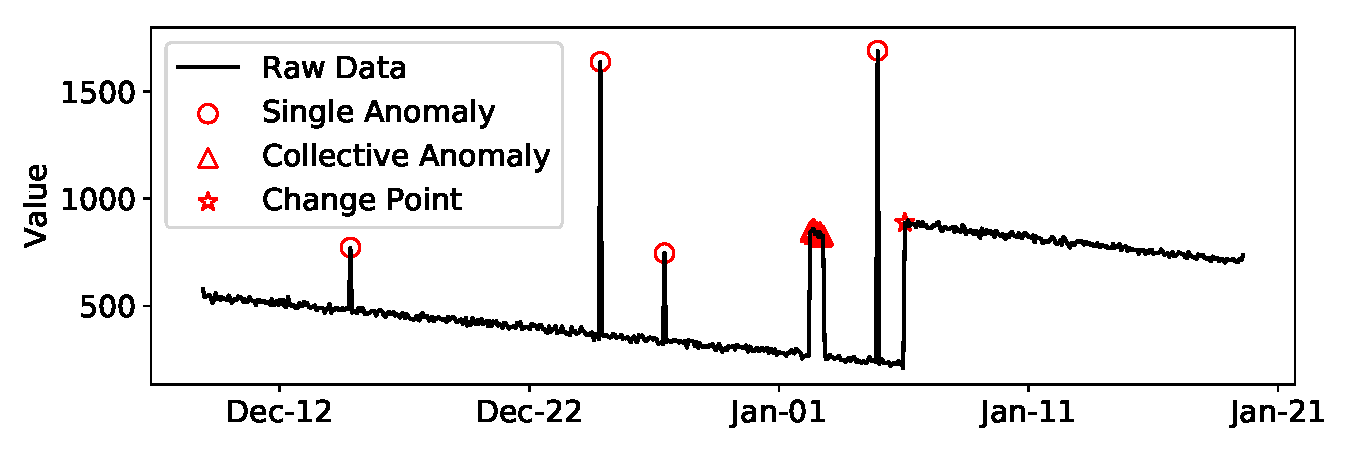
\includegraphics[width=0.8\textwidth]{Part3/Chapter7/figures/data_1_ex.pdf}
	\caption{ : An example of Synthetic dataset.}
	\label{fig: data_1_ex}
\end{figure}

\subsection{Results}
\subsubsection{Experiments on Real Errors}

We evaluate the detection quality our proposal over the real data sets provided by Yahoo and an IoT solution company. Since Yahoo does not record the change points, we only perform anomaly detection on such datasets. Table~\ref{tab:yahoo_data} reports Precision, Recall, F-measure and the number of query to achieve 80\% confidence weight over 50 Yahoo's datasets.\\

We present the notable results in the first part of this table. It is not surprising that Active learning significantly increases CABD's detection quality. Without active learning process, the average precision and recall scores were about 72.7\% and 77.2\% respectively. In some datasets, F-score achieved 100\% on average such as \textit{real\_3} and \textit{real\_6}, meaning that all detected points are totally correct without false. After applying active learning to optimize the probabilistic model, both the precision and recall score were converging to perfect value. The achieve results increased to about 96.8\% and 97.8\% for precision and recall values, respectively. Moreover, the query is very effective shown through low benefit score (0.5 on average). This means labeling a candidate could reveal 2 other abnormal points. \\

In further analysis, we analyze the worst results which are presented in the second part of Table~\ref{tab:yahoo_data}. Intensively investigating into such results, we realize that the false negatives usually occurs at the boundaries of abnormal data, especially at the ends of collective anomalies. \\

From two real IoT datasets shown at the end of Table~\ref{tab:gcz_data_synthetic}, we note that the anomaly detection's recall on average was 100\% without labeling requirement, this means all abnormal points are recognized. However, the overall F-scores of anomaly and change point detection only achieve about 57.3\% and 33.3\% respectively. Based on active learning, the F-score coverages to perfection at 100\% after labeling 1 candidate. These results prove again that our proposal is capable of effectively detecting both anomalies and change points with very few label requirement. %and coverage to high accuracy.
\\

\begin{table}[h]
\small
  \centering
   \small{
   \resizebox{\columnwidth}{!}{%
       \setlength\tabcolsep{2pt}
        \begin{tabular}{c|c|c|c|c|c|c|c}
        \multirow{3}[3]{*}{\textbf{Dataset}} & \multirow{3}[3]{*}{\textbf{\%AD}} & \multicolumn{1}{c|}{\multirow{3}[3]{*}{\textbf{\%CP}}} & \multicolumn{2}{c|}{\textbf{W/O AL}} & \multicolumn{2}{c|}{\textbf{W/ AL}} & \multicolumn{1}{c}{\multirow{3}[3]{*}{\textbf{\makecell{Total\\query}}}} \\
    \cmidrule{4-7}          &       &       & \multicolumn{1}{c|}{\multirow{2}[2]{*}{\textbf{\makecell{AP\\F-score}}}} & \multicolumn{1}{c|}{\multirow{2}[2]{*}{\textbf{\makecell{CP\\F-score}}}} & \multicolumn{1}{c|}{\multirow{2}[2]{*}{\textbf{\makecell{AD\\F-score}}}} & \multicolumn{1}{c|}{\multirow{2}[2]{*}{\textbf{\makecell{CP\\F-score}}}} &  \\
              &       &       &       &       &       &       &  \\
        \midrule
        Synthetic & 12.5  & 9.5   & 38.0  & 39.3  & 67.9  & 83.6  & 38.7 \\
        \midrule
        Yahoo & 1.0   & -     & 44.4  & -      & 80.0  & -     & 5.0 \\
        \midrule
        IoT & 0.8   & 1.0   & 53.7  & 33.3  & 100.0 & 100.0 & 4.0 \\
        \end{tabular}%
        }
      \label{tab:all_evaluation_results}%
       \caption{: Evaluating Anomaly Detection (AD) and Change Point Detection (CP) qualities on Synthetic, Yahoo and IoT datasets.}
       }
\end{table}%


\subsubsection{Experiments on Synthetic Errors}

Next, we evaluate CABD on the synthetic datasets which simulate various anomaly types and change points as real scenarios. Similar to real datasets, the detection qualities (both anomaly and change point detection) are measured in two phases: before and after executing active learning. Table \ref{tab:gcz_data_synthetic} presents the experiment results of varying anomaly and change point proportion. From this table we note that:\\

First, CABD with active learning significantly improves the detection accuracy. The average F-score increases from 38\% to 67.9\% and from 39.3\% to 83.6\% for anomaly and change point detection respectively. Remarkably, the active learning takes more advantage at low anomaly percentage. For example: in dataset with 1\% anomaly such as \textit{ds-1}, the F-score increase by about 80\% from 17.3\% to 97.3\% after learning. Similar results are also found in \textit{ds-6} and \textit{ds-11} datasets. \\

Second, the query selection of active learning is highly effective. The benefit score is about 0.88 on average, that means labeling 12 candidates could recognize 100 abnormal points. As shown in Figure~\ref{fig:comapration_benifit}, regardless the changes in percentage of anomaly and change point, the query benefit is consistent from 0.8 to 0.96. This result demonstrates that the model inputs (score metrics) calculated from Inverse Nearest Neighbor concept are highly related in detecting anomaly and change points. \\

Lastly, as illustrated in Figure~\ref{fig:comapration_AC}, high percentage of anomalies and change points could decrease the efficiency of CABD. In more detail, increasing the anomaly percentage from 1\% to 20\% will decrease the F-score by 27.4\% and 31\% for anomaly and change point detection, respectively. This can be explained that if a single anomaly point is very close to a change point, its spreading pattern based on inverse nearest neighbor will be larger than usual. Thus, the metric score of such point is very likely to a change point. This leads the classification model to conflict when labeling this point as a single anomaly. 

\begin{figure}[h]
	\centering
	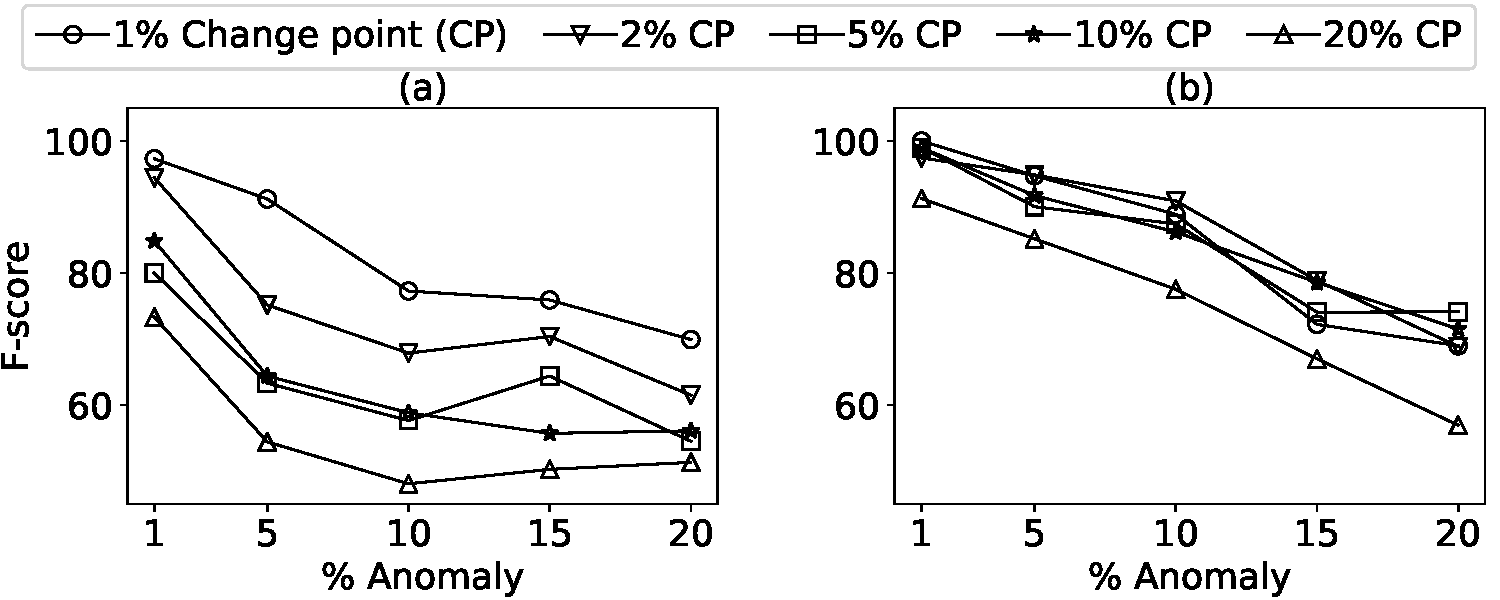
\includegraphics[width=0.8\textwidth]{Part3/Chapter7/figures/new_changeALpercentage.pdf}
	\caption{ : Varying the percentages of anomaly and change point over Synthetic data. From left to right, the two plots show:  (a) Anomaly detection quality, (b) Change point detection quality.}
	\label{fig:comapration_AC}
\end{figure}

\subsubsection{Runtime}
We experimentally compare the runtime of CABD and reviewed algorithms on various data sizes. All evaluations are performed on a computer with following configuration: Intel i5-6200U CPU @ 2.30GHz, 2 Core(s), 4 Logical Processor(s), 8GB of RAM and the operating system is 64-bit Windows 10. Since CABD is an active learning algorithm, labeling time of the end-user is not included. As shown in Figure~\ref{fig:comapration_timerunning}, the runtime of CABD roughly equals that of LOF and is extremely tiny comparing with Numenta or KNN-CAD at all data sizes. More details, with 2000 data points, Numenta and KNN-CAD process in 24.91 and 11.61 seconds, respectively, while the runtime of CABD is only around 0.16 seconds. The similar results are also found in the larger datasets. Numenta and KNN-CAD need 356.03 and 113.02 seconds respectively to detect the anomalies in 20000 data points whereas CABD needs 2.56 seconds. In summary, CABD could provide significant better in both detection quality and running time over the state-of-the-art algorithms.

\begin{figure}[h]
	\centering
	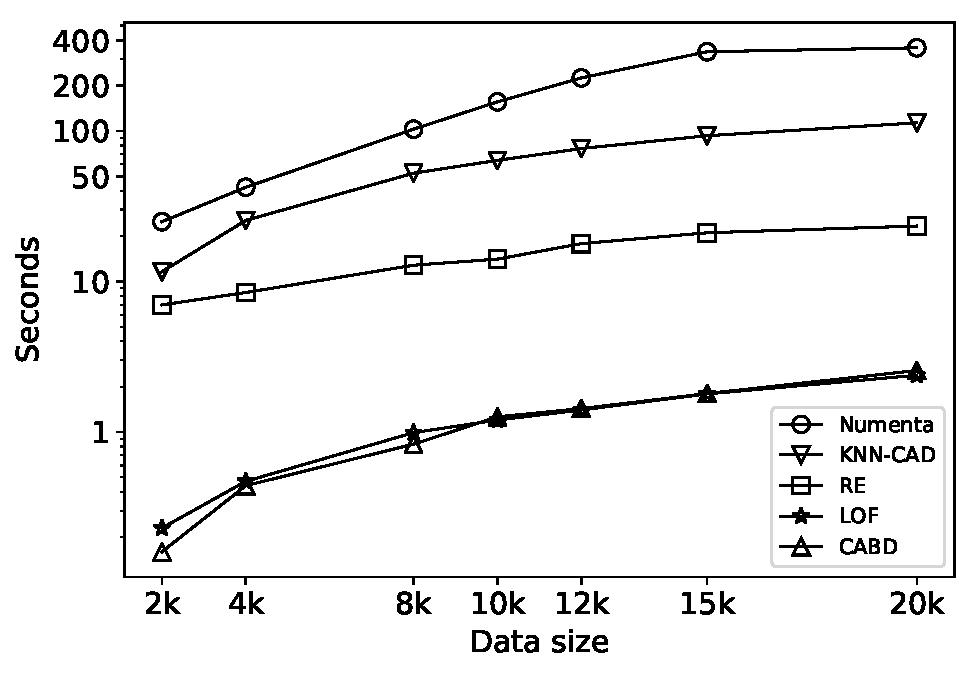
\includegraphics[width=0.6\textwidth]{Part3/Chapter7/figures/time_running_evaluation.pdf}
	\caption{ : Evaluating runtime of common Anomaly Detection Algorithms over different data sizes for Yahoo datasets.}
	\label{fig:comapration_timerunning}
\end{figure}

\subsection{Effectiveness of Active learning}

In our proposal, the Active learning process is an important step to achieve non-parametric algorithm and high accuracy in wide range user-cases. Summarizing evaluation results from Table~\ref{tab:gcz_data_synthetic} and \ref{tab:yahoo_data}, the detection quality of CABD with active learning always outperforms one of non-active learning. For example, the average f-score of anomaly detection on Yahoo datasets increases by 35.3\% from 61.8\% to 97.1\%. This stems from the fact that active learning could optimize the probabilistic classification model to be more accurate. \\

Table~\ref{tab:AL_queryrounds} presents the accuracy score (acc), minimum confident (cof) of the model in each round. The number of correct points (noc) detected from candidate list, which is done in Candidate Estimation step, also reported. From this table, we note that the model may identify all abnormal points (reach 100\% accuracy score) after a few queries.  For example, after 4 queries, the model in $ real\_1 $ dataset reaches 100\% accuracy with 21 data points be distinguished. In some round, the model accuracy decreases after labeling a candidate point. This can be described to the following: in case the abnormal point appears very close a change point pattern, the metric score of this point tends to similar with change point such as high magnitude score, correlation score, and low variance score. Thus, CABD detects the point as a change point. Consequently, labeling this point as an abnormal point will conflict with current mode awareness which leads to decrease mode accuracy. 

\begin{table}[ht]
  \centering
  \small{
        \setlength\tabcolsep{3pt}
        \begin{tabular}{|c|c|c|c|c|c|c|c|c|c|c|}
        \toprule
        \multirow{2}[4]{*}{\textbf{Round}} & \multicolumn{2}{c|}{\textbf{real\_1}} & \multicolumn{2}{c|}{\textbf{real\_23}} & \multicolumn{2}{c|}{\textbf{real\_42}} & \multicolumn{2}{c|}{\textbf{real\_iot\_1}} & \multicolumn{2}{c|}{\textbf{real\_iot\_2}} \\
    \cmidrule{2-11}          & acc   & conf  & acc   & conf  & acc   & conf  & acc   & conf  & acc   & conf \\
        \midrule
        1     & 0.1   & 0.5   & 0.0   & 0.5   & 0.0   & 0.7   & 0.8   & 0.7   & 0.9   & 0.7 \\
        \midrule
        2     & 0.1   & 0.4   & 0.6   & 0.5   & 0.1   & 0.5   & 1.0   & 0.6   & 1.0   & 0.7 \\
        \midrule
        3     & 0.6   & 0.4   & 0.5   & 0.5   & 0.2   & 0.5   & 1.0   & 0.7   & 1.0   & 0.7 \\
        \midrule
        4     & 0.6   & 0.4   & 0.7   & 0.7   & 0.6   & 0.5   & 1.0   & 0.8   & 1.0   & 1.0 \\
        \midrule
        5     & 1.0   & 0.6   & 0.8   & 0.6   & 0.4   & 0.4   &       &       &       &  \\
        \midrule
        6     & 1.0   & 0.6   & 0.8   & 0.5   & 1.0   & 0.6   &       &       &       &  \\
        \midrule
        7     & 1.0   & 0.8   & 1.0   & 0.7   & 1.0   & 0.4   &       &       &       &  \\
        \midrule
        8     &       &       & 1.0   & 0.8   & 1.0   & 0.9   &       &       &       &  \\
        \bottomrule
        \end{tabular}%
      \caption{: Active learning query round}
	\label{tab:AL_queryrounds}%
  }
\end{table}%

%\begin{figure}[h]
%	\centering
%	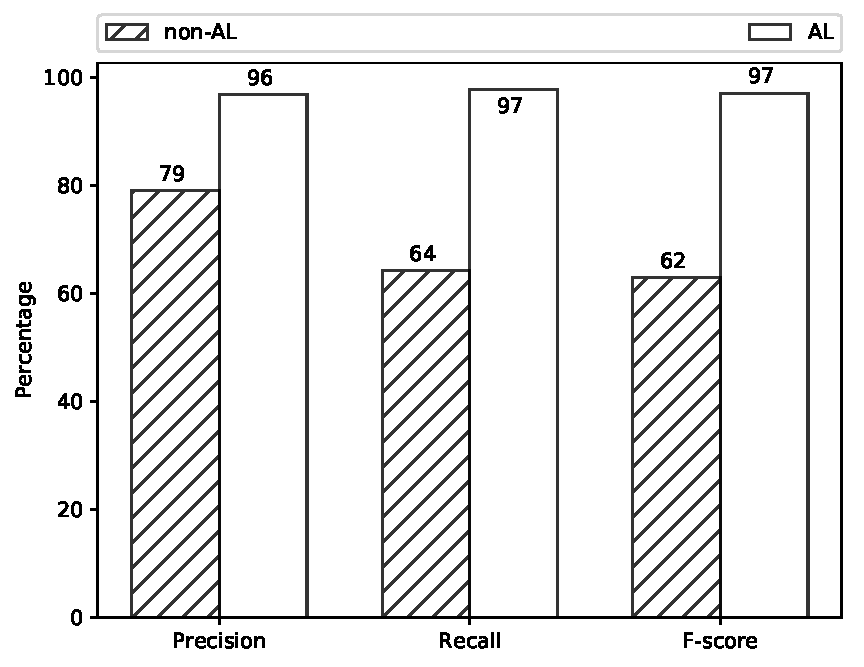
\includegraphics[width=0.5\textwidth]{comparation_percentage.pdf}
%	\caption{ : Comparison the F-score between CABD with and without active learning.}
%	\label{fig:comapration_percentage}
%\end{figure}




\subsection{Effectiveness of INN} 
\par Similarly active learning, Inverse Nearest Neighbor is a novel concept accelerating detection accuracy. Moreover, searching INN is a non-parametric algorithm. This makes INN robust to the sensibility of parameter configurations that is one of common limitations in reviewed algorithms. To demonstrate the efficacy of INN in comparison with KNN, we replace INN by KNN in our evaluation. The appropriate K parameter is determined by bruce-foced searching in range from 0 to data size. Such replacement is evaluated on both real and synthetic data sets. \\

As shown in Figure~\ref{fig:comapration_INNvsKNN_yahoo}, CABD using INN~(CABD-INN) shows better performance in comparison with one using KNN~(CABD-KNN) in both cases (with and without active learning). In details, the f-scores of CABD-KNN are reported around $31\%$ and $48.32\%$ for before and after active learning respectively. Replacing KNN by INN, the f-score significantly increases by 31.68\% to 80\% in case performing AL and by 13.4\% to 44.4\% before performing AL. 

\begin{figure}[h]
	\centering
	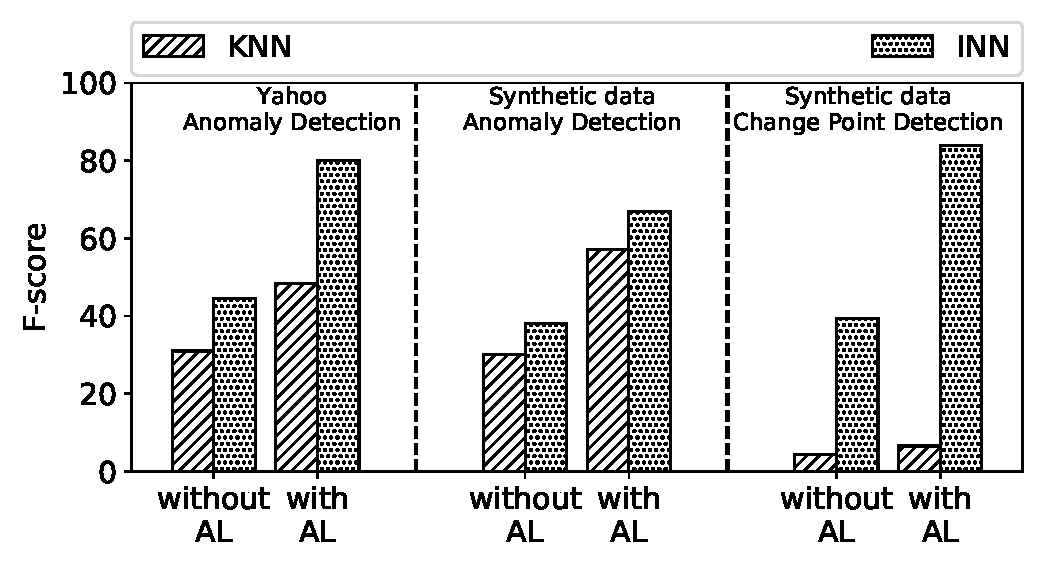
\includegraphics[width=0.8\textwidth]{Part3/Chapter7/figures/INNvsKNN_yahoo.pdf}
	\caption{ : Comparison the effectiveness of INN and KNN in two cases: before and after performing Active learning. From left to right, the two plots show: (a) Anomaly detection quality over Yahoo datasets, (b) Anomaly and change point detection quality over Synthetic datasets.}
	\label{fig:comapration_INNvsKNN_yahoo}
\end{figure}

The same results are found in the evaluation over synthetic datasets. CABD-INN outperforms CABD-KNN in all cases. Especially in change point detection, the f-score of CABD-INN achieves 39.3\% before AL and 83.8\% after AL respectively while that of CABD-KNN are only around 4.38\% and 6.55\%. These results prove again the superiority of INN over KNN. 

\subsection{Enhancing repairing quality}

To minimize the impact of anomalies on data reliability, a repairing process is usually triggered after anomaly detection. We evaluate the integration of our proposal with a recently proposed data-repairing algorithm, Iterative Minimum Repairing (IMR)~\cite{song2015screen,zhang2017time}. The experiment shows how the quality of the automatic data repairs of IMR improves by % randomly labeling 20\% data and 
labeling anomalies with the Active Learning mechanism of CABD. The repairing quality is presented by Root Mean Square (RMS) error that evaluates the distance between ground truth and repaired value. Lower RMS error values indicate better results. Figure~\ref{fig: IMR_optimization} illustrates the experiment over synthetic datasets with varying anomaly and change point percentages. IMR with CABD for the labelling of the data shows significantly better repairing results than the original IMR (based on random values selection) in all datasets. For example, in dataset ds-1 and ds-2, CABD reduces RMS error 4 times from about 74.5 and 85.4 to 16.7 and 18.9, respectively. Moreover, referring to Table~\ref{tab:gcz_data_synthetic}, with CABD, the average number of labelled points for synthetic datasets is 38.72. Given that there are 2000 data points, this means that CABD require the labeling of about 2\% data point to achieve such results. \\

In summary, these results prove the utility of our propose in both improving the repairing quality and in reducing the data labeling effort.

\subsection{Comparison of quality}
We do state-of-the-art a number of anomaly detection method but evaluating all of them is extremely heavy. The algorithms are evaluated including Numenta \cite{ahmad2017unsupervised}, KNN-CAD \cite{burnaev2016conformalized}, ContextOSE \cite{ContextOSE}, Multinomial Relative Entropy \cite{wang2011statistical}, Bayesian Online detection\cite{adams2007bayesian}. The NAB standard profile is used to determine abnormal points relied on anomaly score. The source code and parameter settings for all of the above algorithms are fetched from NAB repository. \\

A comparative analysis of detection quality on all datasets (Yahoo, IoT and Synthetic datasets) reported in Figure~\ref{fig:comapration_USVs_sync} shown that the detection quality presented by F-score of all reviewed algorithms is fairly low when dealing with various anomaly types. The average of F-measure is under 20\% even with the recent algorithms such as Numenta or KNN-CAD. That is, they may not deal with a large number of consecutive errors as well as the present of change points. Contrastingly, CABD always shows significantly better results on all cases (with and without applying active learning). The average F-measure scores before and after active learning on all datasets are about 45.3\% and 82\% respectively. \\

%This result demonstrates that our proposal works well in different anomaly types in wide-range scenarios.  

In a further study, we compare detection quality between CABD and the most common supervised outlier detection algorithms such as 
Angle-Based Outlier Detection (ABOD)~\cite{kriegel2008angle},
Clustering-Based Local Outlier Factor (CBLOF)~\cite{he2003discovering},
Feature Bagging (F-Bag)~\cite{lazarevic2005feature},
Isolation Forest (IF)~\cite{liu2008isolation},
Minimum Covariance Determinant (MCD)~\cite{hardin2004outlier},
Principal Component Analysis (PCA)~\cite{shyu2003novel},
Robust Covariance (R-CoV)~\cite{rousseeuw1999fast}, 
One-Class Support Vector Machines (SVM)~\cite{ma2003time}. 
These algorithms are trained by clean datasets which are eliminated abnormalities. In this evaluation, the source code of such algorithms are obtained from Python toolkit for detecting outlying objects~\cite{pyod}. Figure~\ref{fig:comapration_SVs_yahoo} presents the results on the Yahoo, IoT and synthetic datasets. Again, such results are similar to those in Figure~\ref{fig:comapration_USVs_sync}. That is, CABD always shows the significantly better performance comparing with others. For example, on Yahoo datasets, the average F-score of CABD after active learning is 80\% while the best of others is only 40\% (HBOS algorithm). Similarly, such scores on synthetic datasets are reported about 68\% and 38\% for CABD and best of supervised algorithms (Isolated Forest (IF) algorithm) respectively.

\begin{figure}[h]
	\centering
	\includegraphics[width=0.8\textwidth]{Part3/Chapter7/figures/SVs_compare_yahoo_synthetic.pdf}
	\caption{ : Comparing detection quality with Supervised Anomaly Detection Algorithms over all datasets}
	\label{fig:comapration_SVs_yahoo}
\end{figure}

\begin{figure}[h]
	\centering
	\includegraphics[width=0.8\textwidth]{Part3/Chapter7/figures/SVs_compare_unsuperviced_yahoo.pdf}
	\caption{ : Comparing detection quality with Unsupervised Anomaly Detection Algorithms over all datasets}
	\label{fig:comapration_USVs_sync}
\end{figure}

\section{Related Work}
The same ambition preserves the notable information from data cleaning process. The SCREEN algorithm~\cite{song2015screen}
works under the assumption that the speed of data changes (namely speed constraint) is constraint. This means the $jump$ of values is limited and considered as an anomaly if it is out of a given boundary. Based on such assumption, they propose a solution for stream data to identify and repair the  “jump” values in a given sequence (windows data) w.r.t the speed constraint while minimizing the repair distance. To achieve this goal, the authors introduce a novel concept named “Median Principle” to find the middle point of a specific sequence that is intuitively believed minimizing the repair distance. In addition, to deal with the trade off between choosing the window size and speed constraints. They proposed an adaptive windows size based recently extreme speed constraint (min or max speed). However, the SCREEN can show high performance in repairing single anomaly but hardly handle a collective anomaly. In addition, the repairing results strongly reply on the correctness of initial assumption. Being aware such limitations, a latter algorithm named Iterative Minimum Repairing (IMR)~\cite{zhang2017time} is proposed. The general idea of such algorithm is that combining between labeling some dirty observations and iterative repairing from high to low confidence repairs could enhance the performance. After each iteration, the parameter of the ARX~\cite{park2005outlier} model is calculated to generate the repair candidate list based on the difference of original and inferred data. The data point with minimum difference is repaired. The stop conditions of repairing procedure could be reaching the threshold of convergence or maximum number of iterations. The final goal of CABD, SCREEN and IRM is to preserve the notable information in time series data. But, we try to optimize the anomaly detection procedure while SCREEN and IRM aim to improve repairing procedure. Thus, they are not in our comparison base-line.  \\

In this section, we briefly review the concept of nearest neighbor analysis which has been used in the several contexts of anomaly detection. Such techniques detect the abnormality by examining the distance or similarity between two data instances. Normal data instances occur in dense neighborhoods, while anomalies occur far from their closet neighbors \cite{chandola2009anomaly}. The distance (or similarity) can be calculated in different way. For example: Euclidean distance is the wide usage for continuous attributes in \cite{Breunig:2000:LID:335191.335388}\cite{tang2001robust}\cite{kriegel2009loop}. For categorical attributes, a simple matching coefficient is often used but more complex distance measures can also be used \cite{boriah2008similarity}\cite{chandola2008understanding}. There are two main approaches in Nearest neighbor-based anomaly detection techniques: (1) Using the distance to the k nearest neighbor as anomaly score. (2) Computing the anomaly score from the relative density of each data point.\\

The original idea of nearest neighbor anomaly detection defines the anomaly score of a data instance as its distance to its $ k^{th} $ nearest neighbor in a given data set which is mentioned in \cite{byers1998nearest}. This work also has been applied to detect shorted turns in wind turbin-generators in \cite{guttormsson1999elliptical}. The basic technique is enhanced by researchers in various aspects. For example: The author in \cite{eskin2002geometric}\cite{angiulli2002fast}\cite{zhang2006detecting} calculates anomaly score from the sum of the distance to k nearest neighbors. \cite{knorr1997unified} counts the number of nearest neighbor within d distance as anomaly score. \cite{wu2006outlier} designs a simple sampling technique to reduces the complexity of algorithm. A Resolution Outlier Factor (ROF) was proposed in \cite{fan2006nonparametric}. According to this method, points are outliers or within a cluster depends on the resolution of applied distance thresholds. Conformalized density- and distance-based anomaly detection \cite{burnaev2016conformalized} measure the dissimilarity between observation by combining feature extraction method and conformal paradigm. This was shown to provide effective results for outlier analysis.\\

The density-based anomaly detection is based on the idea: “An instance that lies in a neighborhood with low density is declared to be anomalous while an instance that lies in a dense neighborhood is declared to be normal”. The most well-known algorithm in such technique is Local Outlier Factor (LOF)\cite{Breunig:2000:LID:335191.335388}. For given data instance, the anomaly score is basically the ratio of the average local densities of its k-nearest neighbors over the local density itself.  However, LOF ineffectively detects the regions which are not clearly separated. Several researches were subsequently proposed to extend the concept of LOF. The authors in \cite{jin2006ranking} uses symmetric nearest neighbor relationship to define the outlier score. \cite{tang2002enhancing} introduces a new variation of LOF named Connectivity-based Outlier Factor (COF)\cite{tang2001robust} which can detect the abnormality distributed on arbitrarily shaped clusters. The LOF is also combined with other techniques. For example, the work in \cite{he2002outlier}\cite{he2003discovering} calculate the anomaly score, named Cluster-Based Local Outlier Factor (CBLOF), from local distances to nearby cluster and the size of the clusters. The other method is LOCI, a truly density-based method, using the number of circular neighbors around data point as outlier score. Most of existing nearest neighbor anomaly detections are sensitive to define the k-nearest neighbors. \cite{ha2014robust} propose a new method using instability factor (INS) aiming to overcome the weakness relating the vulnerability of parameter configuration. The enhanced version of INS using “Natural Neighbor” concept is introduced in \cite{huang2016non}.
A more recent proposal is presented in \cite{wang2011statistical} using relative entropy as the distance measurement.\\

Additional algorithms for anomaly detection purpose on time serial data introduce in \cite{Lakhina:2004:DNT:1030194.1015492}\cite{1565683}. Twitter proposes an open-source method named Seasonal Hybrid ESD \cite{hochenbaum2017automatic} using seasonal decomposition and statistical metrics to correctly detect anomalies. Skyline \cite{skyline} and Loda \cite{Pevny2016} use an ensemble of various weak detections or statistical techniques to enhance the detection performance.The other method named KNN-CAD \cite{burnaev2016conformalized} uses a probabilistic model to interpret the distance based on the conformal paradigm. We include evaluation of these methods in our result section.
\par The key advantages of nearest neighbor-based method are unsupervised and independent with data distribution. This means they are purely data-driven \cite{chandola2009anomaly}. However, this method fall in two aspect: (1) it can not handle a sequence of continuous outliers or large collective anomalies due to be sensitive in parameter configuration. (2) It mis-detects the seasonal event as abnormality due to lacking frequency checking.  In contrast, our CABD approach, using new concept named invert nearest neighbor and applying active learning, could not only detect both single and collective anomalies with better accuracy but also highlight the valuable events. 

% \begin{figure}[h]
% 	\centering
% 	\includegraphics[width=0.4\textwidth]{CABDvsIMR.pdf}
% 	\caption{ : Comparing the anomaly detection quality between CABD and IMR over Yahoo and Synthetic datasets.}
% 	\label{fig:comapration_CABDvsIMR}
% \end{figure}



\section{Conclusion}

With the increase in connected devices in IoT, the anomaly detection is becoming increasingly important. We believe anomaly detection represents one of the most significant near-term applications for machine learning in IoT. In this work, we propose a new unsupervised algorithm for anomaly and breakpoint detection. The proposed method combines the novel concept named invert nearest neighbor and active learning. Unlike the most of previous outlier detection approached, our algorithm not only effectively detect s both single and collective anomaly but also preserves and highlights breakpoint. Moreover, we solve the challenge regarding the sensitiveness of parameters in existing methods by applying active learning to adapt the parameters. Experimental results clearly indicate that the effectiveness of the proposed method for real IoT user-cases. To further prove the effectiveness of invert nearest neighbor and active learning, we will apply them in not only anomaly detection but also clustering algorithms for future studies. 




\chapter{An Energy Efficient Sampling Algorithm in Massive IoT} \label{ch:smart_freq}
\section{Introduction}

\section{Related Work}
Energy efficiency for constraint devices is a highly interest topic in the context of Internet of Things and can strongly impact on the quality of IoT services. For instance, in IOT agriculture scenario where IoT devices are widely distributed in a large region, optimizing the energy consumption may extend the device life circle as well as significantly reducing the maintenance cost.\\

Considering the fact that waking-up, collecting and pre-processing cost consume a small proportion of energy comparing with transmitting. Thus, energy could be saved by not transmitted unneeded samples, that is also the goal of adaptive sampling approach. The basic idea of adaptive sampling technique is to adapt the sampling rate to the change of observation based on certain criteria  while ensuring the precision  of outcome information []. In this section, we catalog the adaptive sampling approaches relied on such criteria.
\par \textit{Send-on-delta sampling}: is the most commonly used in wireless networks. The original of such approach is the level-crossing sampling at late 1950s based on the idea ``the most suitable sampling is by transmission of only significant data, as the new value obtained when the signal is changed by a given incremen'' \cite{ellis1959extension}. Due to its popularity, there are various temps expressing this strategy such as event-based sampling \cite{940692},  magnitude-driven sampling \cite{persson2001event} or deadbands \cite{otanez2002using}. Formally, given threshold $ \delta $, a message has value $ y_i $ at $ t_i $ is sent if and only if 
\begin{equation}\label{key}
(y_i - y_k) > \delta
\end{equation}
with $ y_k $ is the last message be sent at $ t_k $. To prevent babbling-idiot failure on such approach, the min and max sending time, denoted by $ T_L $ and $ T_H $ respectively, are defined as the boundary of sampling interval ($ T_L \leq t_i - t_l \leq T_H $)\\

\textit{Integral Sampling} uses the concept of integral or energy of the error to deal with small oscillations in the signal. The message is sent if the accumulated error of sampling, denoted by CES, is greater than a pre-defined threshold $ \xi $. The min and max-send-time are also applied. The CES value of a signal $ x(t) $ is the deference between $ x(t) $ and accumulated value from the most recent sample $ x(t_k) $. 
\begin{equation}\label{CES}
CES_{x_t} = \displaystyle\int\limits_{t_i}^{t_{i-1}} [x(t) - x(t_{t-1})]^{2}dt
\end{equation}
where $ i=1,2,...,n $ is the number of sample taken from $ t_0 $ to $ t_n $ \cite{miskowicz2005sampling}\\

\textit{Predictor-based sampling} uses a model to predict the next measure based on the past values. The message $ x(t) $ is sent if it significantly differs with  the predicted value $ \hat{x}(t) $. The criterion of the difference may reuse either sen-on-data or interval sampling. The model is build from a simplified statistic using linear extrapolation \cite{suh2007send}. To maintain the information quality, the predictor is also used in receiver to extrapolates the signal value until receiving the new message. However, updating receiver predictor requires at least 2 samples. This reduces the efficiency of such approach.\\

\textit{Gradient-based integral sampling} is an extension of integral sampling approach with the optimization of wake-up energy consumption. This method bases on the fact that waking-up device consumes considerably larger than collecting message. Thus, the next wake-up time is automatically adjusted to the current gradient of the signal \cite{ploennigs2009comparison}. To the avoid the worst scenario which the signal gradient is zero, a max-sleep-time is defined. \\

\textit{Sigmoid-based sampling} uses a sigmoid function to estimate the change of sampling rate based on the the variance of the last windowed signal \cite{shu2017energy} \cite{alippi2010adaptive}. Let denote the last message be $ x(t) $ belonging a signal window size $ W $, the variance is the absolute difference of between $ x(t) $ and $ x(t-1) $ over the average value of $ W $. Then such variance is compared with a pre-determined threshold before calculating the new sampling rate is the multiplication of current race and the sigmoid function of such variance. Such new rate is  changing rate is limited from 0 to 2 as a result of sigmoid function properties. 

%%%%%%%%%%%%%%%%%%%%%%%%%%%%%%%%%%%%%%%%%%%%%%%%%%%%%%%%%%%%%%%%%%%%%%%%%%%%%%%%%%%%%%%%%%%%%%%%%%%%%%%%%%%%%%%%%%%%%%%%%%%%%%%%%%%%%%%%%%%%%%%%%%%%%%%%%%%%%%%%%%%%%%%%%%%%%%%%%%%%%%%%%%%%%%%%%%%%%%%%%%%%%%%%%%%%%%
\section{Adaptive Sampling Algorithm}
Unlike the existing adaptive sampling algorithms that share a vulnerability to configuration parameters, we propose a light-weight adaptive frequency for improving the power efficiency based on user's desire while maximizing the sampled data. In this section, we first present the overall algorithm. Then, we briefly explain each step along with related definitions.

\subsection{Preliminaries}
\textbf{Definition 1}(Absolute first difference). The absolute value of first difference of $ \theta_{i}(p) $, denoted as $ \triangle\theta_i(p) $, which is defined that:
\begin{equation}\label{First_difference}
\triangle\theta_i(p) = |\theta_{i}(p) - \theta_{i-1}(p)|,\, i = 1, 2, 3, ..., n
\end{equation}

\textbf{Definition 2}(Absolute Second difference). The absolute value of second difference of  $ \theta_{i}(p) $, denoted as $ \triangle " \theta_i(p) $, which is defined that:
\begin{equation}\label{Second_difference}
\triangle"\theta_i(p) = |\triangle\theta_{i}(p) - \triangle\theta_{i-1}(p)|,\, i = 1, 2, 3, ..., n
\end{equation}

\subsection{Overview Algorithm}
The light-weigh adaptive sampling algorithm is designed to optimize power utilization of constrained devices in IoT. Given the desire power saving level, the algorithm maximize the accuracy of sample data at such level.  \\

The general idea of our proposed algorithm is to dynamically adapt the sampling frequency according to the observation changes. Obviously, a higher frequency is strongly preferred to context awareness when there are significant changes in the observation. For example, in forest fire warning service, the sudden increase of temperature is considered as notable events. Increasing frequency may help to deeper investigating such events. In contrast, if the observed value is hardly fluctuate, a decrease in frequency is desired to save energy in data sampling, processing and transmission. \\

To archive these assumptions, a enhanced sigmoid function is exploited to quickly adapt the sampling frequency, which is described as: 
\begin{equation}\label{Fchange}
 f_{change} = n + \frac{1-n}{1 + e^{-n*D}}
\end{equation}
with:
\begin{equation}\label{D}
 D = \frac{\triangle\theta_i(X_i) - \frac{n+1}{2}*(\frac{1}{N}\sum_{j=i-N}^{i} \triangle\theta_i(X_j))}{\frac{1}{N}\sum_{j=i-N}^{i} \triangle\theta_i(X_j)}
\end{equation}

In the equation \ref{Fchange}, n is the user desire of power saving; and D presents the sudden change of coming data comparing with sliding window based N most recent data. It is reasonable to compare the change of 
the absolute difference between $ X_i $'s absolute first difference over the mean value of such difference of last N data points. If D is sufficiently large, this means the current change is overwhelming in comparison with recent history. Then the sampling frequency is adapted with this change. In contrast, if the value of D is negative, which means the values change is not large enough, the sampling frequency can be reduced to save the device resources. \\

As the result of extended sigmoid function, the theoretical value of new frequency is limit in a certain range from standard frequency (assuming to equal 1) to user desire (n), that is, regardless the value of D, new frequency denoted by y(D) is always in defined boundary. This barrier is vital in constrained network such as LPWAN, SIGFOX whereas the boundary of sending messages interval is strictly limited. The presentation of y(D) function is illustrated in figure 1. It is found that the value of y is highly change when the D value is in range from -1 to 1,that is, change of lasted sampled data is higher from $ \frac{n-1}{2} $ to $ \frac{n+3}{2} $ times than the mean of this change in history. For the rest value of D, the y(D) converges to border of its boundary. Hence, the new sampling frequency for the next iteration is capable of adapting to change in lasted data and bounded in desired ranges, which satisfy the needs for a effective frequency algorithm as well as energy conservation. \\

Our proposed algorithm manipulates the extended sigmoid function corresponding with natural sampling process which is robust with faulty in sensed data. This scheme ensures that the new frequency is calculated not only based on lasted sensed data but also historical data which presents the overall data trend. In more detail, a anomaly value in sensor reading, which may be significantly higher than the average change recently, does not strongly impact on the next sampling frequency. The frequency only significantly changes when there are consecutive changes in obtained data. As the result, our approach effectively determine whether the device energy is either consumed or conserved based on the trend of the sensed data rather than uncertain changes on last value. 
The pseudo code for implement our proposal is presented as below:


\begin{table}[h]
	\centering
	\begin{tabular}{l}
		\toprule
		\textbf{Algorithm 1:} Adaptive Frequency for of newest data point $ X_i $\\
		\midrule
		\textbf{Input: } $ X_i $, window size $ N = 50 $ \\
		\textbf{Output:} New frequency $ f_{new} $ \\
		1.~ Initializing: Window W = \{$ X_{i-N}, X_{i-N+1}, .... , X_i $\}	 \\
		2.~ Calculating changing degree: \\
		\hspace{10mm}		$ D = \frac{\triangle\theta_i(X_i) - \frac{n+1}{2}*(\frac{1}{N}\sum_{j=i-N}^{i} \triangle\theta_i(X_j))}{\frac{1}{N}\sum_{j=i-N}^{i} \triangle\theta_i(X_j)} $ \\
		3.~ Calculating the new frequency: \\
		\hspace{10mm} 		$ f_{new} = n + \frac{1-n}{1 + e^{-n*D}} $\\
		\textbf{return $ f_{new} $}
	\end{tabular}
	\label{tab:AL_1}
\end{table}


\section{Experimental Evaluation}
In this section, we present the evaluation result to demonstrate the efficiency of our proposal on both real and synthetic dataset. We also experimentally compare with the common anomaly detection approaches using NAB \cite{lavin2015evaluating}. At the end, we discuss the importance of Active learning in CABD.
%In this section, we empirically evaluate the quality and efficiency of our proposal on both real and synthetic dataset. We demonstrate that:
%\begin{itemize}
%	\item CABD effectively detect both single and collective anomalies which need to be removed.
%	\item CABD quickly identify the key deviation event which also known as break point.  
%	\item Applying active learning significantly improves the CABD’s accuracy. 
%\end{itemize}
%We briefly describe each of these goals below

%\subsection{User studies}
%\subsubsection{User study 1: Tank Monitoring}
%\subsubsection{User study 2: Humility Monitoring}


\subsection{Metric of Measurement}
For evaluating the efficiency of proposed algorithm, we use two metric:
\begin{itemize}
\item Normalized Mean Error (NME) to indicate the overall goodness of fit after normalizing between the original signal and reconstructed signal from sampled data. This factor is defined as:
\begin{equation}\label{NME}
NME = \frac{1}{n}\sum_{i=1}^{n} |\hat{x}_i - x_i | * 100\%
\end{equation}
with $ \hat{x}_i $ denotes the normalized \textit{i}th data in the reconstructed signal, $ x_i $ represents the normalized \textit{i}th data in the original signal and n is the size of signal.
\item Resource Saving Factor (RSF) to indicate the conserved resources based on the reduce in transmitted messages be defined as: 
\begin{equation}\label{RSF}
RSF = \frac{\hat{m}}{n}
\end{equation}
with m and n are the size of sampled data and original data respectively.
\end{itemize}
  
\subsection{Benchmark Datasets}
\textit{National Oceanic and Atmospheric Administration (NOAA) datasets: } The NOAA provides a set of real-time data about water-quality from a place named "Jamestown". In order to reasonably compare with state-of-the-art approaches, we choose the same dataset and monitoring duration ranges with them which are turbidity and DO from 15 December 2016 to 15 March 2017. \\

\textit{IoT datasets: } The data is collected from 2 real CO2 sensors deployed in the working space with the sampling interval of 1h for a sample. 

\subsection{Evaluative Simulation}

To assess our proposal performance, we simulate the evaluation process closing with real deployment on device. First, the initial sampling frequency is set to the original frequency of dataset. Then the next sampling is calculated by the algorithm. We derive the data value for this sampling from original dataset by using a linear interpolation method. The process is repeated until the next sampling is out of original dataset. The new obtained dataset by our method is up-sampled to the size with original dataset  and normalized before calculating the metric of measurement. The process is presented in the algorithm 2. \\
\begin{table}[h]
	\centering
	\begin{tabular}{l}
		\toprule
		\textbf{Algorithm 2:} Evaluation Process\\
		\midrule
		\textbf{Input: } Dataset X, Window size N, Saving desire n \\
		\textbf{Output:} $ NME, RFS $ \\
		1.~ $ f_{curr} \leftarrow f_{const}$   \\
		2.~ Y = [ $ X_0, X_i, ...., X_n $ ], i = N \\
		3.~ \textbf{While} $ i < size(X) $ \textbf{do} \\
		\hspace{10mm}$
		\left \|  
		\begin{tabular}{l}
		$ f_{new} \leftarrow $ MyAL($ Y, N ,n $) \\
		$ X_{next} \leftarrow $ Interpolation($ X, f_{new} $)\\
		$ f_{curr} \leftarrow f_{new} $\\
		$ Y = Y \cup \{X_{next}\} $\\
		$ i = i + \frac{1}{f_{new}} $\\
		
		\end{tabular}
		\right .
		$\\
		4.~ $ \hat{X} \leftarrow UpSample(Y) $  \\
		\hspace{5mm}$ \hat{X}_{norm} \leftarrow Normalize(\hat{X}) $  \\
		\hspace{5mm}$ X_{norm} \leftarrow Normalize(X) $  \\
		\textbf{Return $ NME(X_{norm}, \hat{X}_{norm}),  RSF(Y,X) $}
		
	\end{tabular}
\end{table}

\subsection{Results}

\subsubsection{Varying user desire n}

\begin{figure*}[h]
	\centering
	\includegraphics[width=0.95\textwidth]{Part3/Chapter8/figures/result_various_n.pdf}
	\caption{ : Varying user desire n, over DO dataset with window size = 50.}
	\label{fig: various_n}
\end{figure*}

Figure \ref{fig: various_n} present the result on varying user desire n, for DO database with fix window size equals 50. First, as shown in figure \ref{fig: various_n} (a), our proposal shows better resource saving with the increase of user desire n. This means more saving desire leads to less transmitted message. Setting n to 1 leads to the new frequency always equals the origin frequency. As a result, the RSF value equals 0 due to no saving resource. 
Remarkably, the RSF value increase at low n value from 1 to 6 but it slightly coverages to a stable level. This happens mainly because the n value is considered as the upper asymptote of the frequency and does not strongly impact on the algorithm output. At an sufficient large n, the RSF value will be stable. \\%The similar result are also observed in real IoT dataset. \\

\begin{figure*}[h]
	\centering
	\includegraphics[width=0.9\textwidth]{Part3/Chapter8/figures/result_various_n_iot.pdf}
	\caption{ : Varying user desire n, over DO dataset with window size = 50.}
	\label{fig: various_n_iot}
\end{figure*}

It is not surprising that the change of MSE and RFS is similar while increasing n value. This is illustrated in figure \ref{fig: various_n} (b) wherein the MSE value is significant increase from 0 to 5 with the increase of n from 1 to 6 then it slowly coverage to stable value, since the MSE is proportional to RFS. This could be explained that higher RFS means less data is sampled and transmitted. Therefore, the reconstructed data is more different with original data. This leads to the increase of MSE. \\
In summary, as presented in Figure \ref{fig: various_n} and \ref{fig: various_n_iot} over the DO and temperature datasets, our proposal is capable of not only preserving the device's resources based on user desire but also being robust with excessively large desired configuration. 

\subsubsection{Varying window size N}

\begin{figure*}[h]
	\centering
	\includegraphics[width=0.9\textwidth]{Part3/Chapter8/figures/result_various_windowsize.pdf}
	\caption{ : Varying user desire n, over DO dataset with window size = 50.}
	\label{fig: various_ws}
\end{figure*}

Figure \ref{fig: various_ws} reports the result by varying the window size ws for different n value on DO dataset. As illustrated, we note that both the RSF and MSE value is independent with ws configuration. While increase the window size from 20 to 100, the RSF is stable around a constant value. For example:......... This results from the superiority of D function. In more detail, the D function compares the current changes degree with the mean of first derivate of historical data. By increasing window size to obtain more history does not strongly impact on this mean, that is, the optimized frequency is well-balanced with the increase of window size. The similar result for Turnity dataset is presented in figure \ref{fig: various_ws_iot}. This result again consolidates the effectiveness and consistency of our algorithm.

\begin{figure*}[h]
	\centering
	\includegraphics[width=0.9\textwidth]{Part3/Chapter8/figures/result_various_windowsize_iot.pdf}
	\caption{ : Varying user desire n, over DO dataset with window size = 50.}
	\label{fig: various_ws_iot}
\end{figure*}

\subsection{Comparison of Results}
We do state-of-the-art a number of adapting sampling algorithm for saving energy but evaluating all of them is extremely heavy. Hence, the compared algorithms are DDASA \cite{shu2017energy}, ASA \cite{alippi2010adaptive} which are the most related with our approach. For transparency, The competitor results are derived from original paper. In order to obtain NME value with the sample size of these results, we execute our algorithm with various user desire value. The estimated NME is calculated by interpolation method.\\

A comparative analysis of NME on DO dataset is presented in table \ref{tab: performance comaprison}. Considering the fact that larger number of sample will definitely consume more energy to collect, store and transmit data. As illustrated, our proposal shows superiority  over the competitors in case of high saving energy. To reduce original dataset to 297 and 421 samples,  the NME values of our approach are around 4.96\% and 4.07\% in comparison with 9.99\% and 8.43 \% of DDASA respectively. This means that the reconstructed data from our selective points is more likely to original data than others. Moreover, our approach is more consistent and robust than the competitor while dealing with high power saving scenario. This is demonstrated by the minor change of NME while reducing the number of sample. In more detail, our NME variance is around 0.79 comparing with 13.6 of DDASA while decrease the sample size from 1064 to 297.\\

In summary, comparing with other approaches, our algorithm has better performance which is demonstrated by lower and more consistent in MSE value. 
%\begin{table*}[h]
%	\centering
%\begin{tabular}{l*{6}{c}r}
%	              & DDASA & DDASA & DDASA & DDASA & ASA & DDASA &Fixed Rate   \\
%	              & (t=0.07) & (t=0.03) & (t=0.02) & (t=0.015) & & (t=0.01)& Sampling  \\
%	\hline
%	Number of Samples & 146 & 297 & 421 & 548 & 637 & 1064 & 2182   \\
%	NME            & 11.7 \% & 9.99 \% & 8.43 \% & 5.31 \% & 5.52 \% & 1.62 \%&  0   \\
%	AFO NME         &7.16 \%& 4.96  \%&  4.07 \% &  4.37 \% &  3.86 \% & 2.84 \%&  0\\
%\end{tabular}
%		\caption{: Performance comparison.}
%\label{tab:gcz_data_synthetic}%
%\end{table*}%

\begin{table*}[h]
	\centering
	\begin{tabular}{l*{6}{c}r}
		&  & DDASA & DDASA & DDASA & ASA & DDASA &Fixed Rate   \\
		&  & (t=0.03) & (t=0.02) & (t=0.015) & & (t=0.01)& Sampling  \\
		\hline
		Number of Samples &  & 297 & 421 & 548 & 637 & 1064 & 2182   \\
		Competitor's NME            &   & 9.99 \% & 8.43 \% & 5.31 \% & 5.52 \% & 1.62 \%&  0   \\
		AFO NME         & & 4.96  \%&  4.07 \% &  4.37 \% &  3.86 \% & 2.84 \%&  0\\
	\end{tabular}
	\caption{: Performance comparison.}
	\label{tab: performance comaprison}%
\end{table*}%

\section{Conclusion}

\chapter*{Conclusion of Part \ref{pa:part3}}
.......... To be compeleted ................


% \cleardoublepage\pagestyle{empty}\mbox{}\cleardoublepage
\addtocontents{toc}{\protect\addvspace{2.25em}}
\clearpage\pdfbookmark[-1]{Conclusions and Future Perspectives}{conclusions}
% \chapter{Conclusions}
% Conclusion and Perspectives
% \clearpage
\chapter{Conclusions and Outlook}
%\minitoc
\label{ch:CFP}
% \lipsum[1-5]
\section{Conclusion}











\appendix
%\clearpage
\chapter{R\'{e}sum\'{e} de la Th\`{e}se en Fran\c{c}ais}
%\section{Introduction}
%Avec le développement de la technologie d'accès sans fil ainsi que l'explosion des appareils mobiles (tels que les smartphones et les tablettes), le réseau mobile de prochaine génération n'est pas seulement limité à fournir des services vocaux traditionnels, mais aussi des services de données. En d'autres termes, il évolue vers des systèmes tout-IP. En fait, les services de données mobiles sont devenus une partie essentielle de la vie de nombreux consommateurs [1, 2]. Par conséquent, le trafic de données mobiles a été presque doublé chaque année au cours de ces dernières années [1, 6]. Cette tendance devrait se poursuivre dans les années à venir, notamment avec le déploiement des réseaux de quatrième génération (4G). Malgré l'augmentation du volume de trafic, le chiffre d'affaires moyen par utilisateur est en chute libre [7]. En outre, les nœuds mobiles peuvent souvent changer leur point d'attache au réseau. La gestion de la mobilité IP est donc un concept essentiel pour répondre à la demande de connectivité d'Internet omniprésente ainsi que des nouvelles exigences en matière de services, tels qu'un handover transparent sur des réseaux hétérogènes, une qualité constante de l'expérience et des contraintes strictes de retard.
%
%Dans ce contexte, MIPv6, le premier protocole de mobilité normalisé par l'IETF pour les réseaux IPv6, maintient l'accessibilité du terminal mobile quand il est loin de la maison. En d'autres termes, MIPv6 permet de communiquer avec un terminal mobile quelque soit l'endroit où il se trouve. Il se fait par l'introduction d'une entité centrale, à savoir l'Agent Mère (Home Agent - HA) situé au réseau de la maison d'un nœud mobile (mobile node - MN), ce qui est un point d'ancre topologique de l'adresse IP d'origine du MN (l'adresse du domicile - Home Address). Grâce à son adresse du domicile, le MN peut communiquer indépendamment de son emplacement actuel dans l'Internet. Cependant, dans MIPv6, le MN doit effectuer la signalisation liée à la mobilité, cela signifie que la pile de protocole MIPv6 est nécessaire au MN. Il est le principal obstacle au déploiement de MIPv6 dans le monde réel. Pour cette raison, PMIPv6, comme un protocole de gestion de la mobilité basée sur le réseau, permet d'éviter la mise en place supplémentaire dans le MN de sorte que le MN peut être simple. En d'autres termes, la mobilité peut être transparente offerte à tous les MNs existants.
%
%Les opérateurs des réseaux mobiles sont mis au défi par l'augmentation du trafic de données mobiles (en particulier le trafic de vidéo) et les nouvelles exigences, par exemple, fournir une connectivité partout et à tout moment avec la cohérence de l'expérience d'utilisateur, tout en préservant l'économie de leurs réseaux et de créer de nouvelles opportunités pour la croissance de revenus. Face à ces défis, les opérateurs cherchent des solutions innovantes pour améliorer la performance et l'efficacité du réseau, ainsi que réduire le coût dépensé sur le fonctionnement et la maintenance du réseau. Deux axes majeurs sont: i) l'augmentation de la capacité de système de communication sans fil; et ii) la conception et la mise en œuvre d'un système efficace de transférer de données. En ce qui concerne le premier aspect, l'augmentation dramatique de la capacité des réseaux radio du haut débit viendra avec la mise en œuvre de nouvelles technologies sans fil telles que WiMAX, HSPA, et LTE. Cependant, le spectre pour les opérateurs est à la fois limité et trop cher. Ainsi, ils cherchent à différentes méthodes pour augmenter la capacité du système comme le déploiement des cellules femto et pico, et la sélection du trafic déchargé entre les spectres sans licence. Regardant le deuxième aspect, l'objectif est de simplifier l'architecture de réseau, ainsi que d'optimiser le coût de transmission de données. En conséquence, le réseau mobile est en train d'évoluer vers une architecture plate. Un exemple est l'architecture LIPA/SIPTO définie par le 3GPP. Suivant la même idée, l'IETF a récemment affrété un groupe de travail de gestion de la mobilité, appelé DMM (Distributed Mobility Management), qui précise les solutions pour résoudre les problèmes et les limites de la gestion de la mobilité centralisée. En fait, la gestion de la mobilité IP traditionnelle (par exemple, MIPv6 et PMIPv6) s'appuie sur l'approche de gestion de la mobilité centralisée, donc, soulève plusieurs problèmes pour les opérateurs tels que l'utilisation inefficace des ressources, une mauvaise performance, et le problème d'évolutivité lorsqu'on considère un grand nombre des appareils mobiles et leur demande de trafic [8, 9, 10]. DMM est une des solutions pour aider les opérateurs mobiles à répondre à ces limites.
%
%
%Comme l'Internet est largement déployé et répartis sur une grande surface, il offre une grande variété de ressources communs et de services d'information communs. Dans un monde partagé, le service de communication de groupe, qui se réfère à la capacité d'envoyer de données à plusieurs récepteurs en même temps, naturellement deviens de plus en plus important, en particulier dans certains domaines comme la distribution de multimédia, les jeux et les services financiers, etc. Dans ce contexte, l'évolutivité et la bande passante efficacité du routage multicast rend multicast une remarquable solution du point de vue de l'application pour faire face à un grand nombre de trafic (notamment, dans des environnements mobiles où les utilisateurs partagent généralement des bandes de fréquences et la capacité limitée [11]). Mais l'un des principaux défis pour le support de multicast est lorsque la mobilité est considérée. Il vient du fait que les protocoles de multicast ont été crées pour les réseaux fixes. En tant que tel, il soulève des problèmes à cause de l'interaction entre les protocoles de multicast et les protocoles de mobilité IP. Ces problèmes sont l'interruption de service, la perte de paquets, le gaspillage de ressources, le routage non optimal, et la duplication de paquets.
%
%
%En ce qui concerne la mobilité multicast IP, après plus d'une décennie d'efforts de recherche et développement, nombreuses approches ont été proposées, mais la plupart d'entre eux sont basés sur les protocoles de gestion de mobilité basés sur le client comme MIPv6. Cependant, le principal inconvénient de ces protocoles est qu'ils nécessitent le MN pour modifier sa pile IP pour participer dans le processus de signalisation de mobilité. En outre, les approches antérieures multicast IP ne peuvent pas être appliquées directement à une gestion de mobilité basée sur le réseau, dans lequel le MN n'est pas au courant de processus de la mobilité. Pour résoudre les problèmes mentionnés ci-dessus, l'IETF a travaillé dans différentes solutions mettant en évidence la différence entre la source et l'auditeur. Cependant, les solutions proposées restent incapables de résoudre les problèmes de l'évolutivité, de l'optimisation de la performance et la compatibilité avec la mobilité unicast en même temps. En DMM, il n'y a pas de solution complète pour la mobilité du terminal multicast.
%
%Il est généralement reconnu que la solution proposée ne peut pas être largement acceptée sans les résultats d'une expérimentation. La validation peut être obtenue par différentes méthodes, chacune avec ses avantages et ses limitations. Dans le domaine de la recherche en réseau, la fiabilité des résultats est l'un des problèmes les plus critiques. Dans ce contexte, la méthode la plus largement utilisée - simulation - manque parfois de crédibilité. La méthode moins utilisée mais la plus crédible - un banc d'essai réel - est trop chère et difficile à l'échelle et à gérer.
%
%Dans cette thèse, notre objectif principal est de faire face aux problèmes liés à la mobilité du nœud multicast. Les solutions sont proposées dans le cadre de l'évolution de la direction actuelle de la mobilité IP : à partir de la gestion mobilité orientée client vers la gestion de la mobilité orientée réseau, et aussi à partir de la gestion centralisée vers la gestion distribuée de la mobilité. Plus précisément, pour un domaine PMIPv6, nous introduisons une méthode pour réduire l'interruption de service et le gaspillage de ressources. Nous présentons ensuite une solution du point de vue de l'équilibrage de charge pour régler les problèmes de l'interruption de service et la duplication de paquets. Comme DMM n'a pas été normalisé, nous proposons une solution de mobilité inter-domaine, qui peut être considérée comme une étape dans l'évolution de PMIP vers DMM. Enfin, nous convergeons vers une architecture finale dans un domaine DMM qui peut offrir divers avantages et résoudre la plupart des problèmes liés à la mobilité des clients multicast. Tout au long de cette thèse, un banc d'essai proche d’un réseau réel est utilisé pour démontrer des résultats réalistes.
%
%\section{Technologies de Référence et Défis}
%\subsection{Multicast IP}
%Contrairement au modèle traditionnel de communication où les données sont envoyées à partir d'une source vers une destination (appelé unicast ou communication un à un) ou à tous les nœuds dans un portée spécifique (broadcast), la technologie multicast permet la transmission de données à un ensemble d'utilisateurs qui sont intéressé à recevoir le même contenu en même temps. En utilisant la technologie multicast, l'expéditeur a seulement besoin d'envoyer une copie unique de données pour accéder à tous les membres du groupe, au lieu de l'envoi d'une copie séparée pour chaque récepteur. Les routeurs intermédiaires alors reproduisent les paquets de données jusqu'à ce qu'ils atteignent les récepteurs. En conséquence, le multicast apporte certains avantages par rapport à la diffusion individuelle (unicast) et le broadcast, tels que la réduction de la charge du serveur et  l'élimination de trafic redondant, donc améliorant l'utilisation ensemble des ressources [28].
%
%Afin de fournir un service multicast, deux groupes de protocole doivent être déployés: les protocoles stations-routeurs et les protocoles de routage. Les protocoles stations-routeurs permettent aux clients de rejoindre dynamiquement / quitter le groupe ainsi qu'aux routeurs de multicast (MR) d'être conscients des récepteurs intéressés et de gérer les abonnements des clients. Les protocoles de routage multicast permettent une collection de routeurs  (MRs) de construire des arbres de distribution pour acheminer le trafic multicast à partir des sources de tous les membres d'un groupe multicast. Les protocoles stations-routeurs, selon la version IP, sont Internet Group Management Protocol (IGMP) [34] pour IPv4 et Multicast Listener Discovery (MLD) [35] pour IPv6. En ce qui concerne les protocoles de routage, chaque protocole utilise son algorithme de routage pour construire les arbres de distribution. Dans cette thèse, nous considérons le PIM-SM (Protocol Independent Multicast - Spare Mode) et une version améliorée de PIM-SM pour la source spécifique (PIM-SSM [41]) comme le protocole de référence. Cependant, les solutions proposées ne sont pas limitées à ce protocole. En outre, le proxy Multicast Listener Discovery (MLD) qui est un protocole léger peut être utilisé pour simplifier la conception et la mise en œuvre du routeur. Les proxies peuvent être placés entre le routeur et le client. La fonction de proxy permet à un nœud d'apparaître comme un routeur pour les clients « en aval » et en tant qu'un client pour le MR « en amont ». Par conséquent, du point de vue pratique, nous nous concentrons sur le scénario où la fonction proxy est déployée au niveau du routeur dans le réseau d'accès.
%
%\begin{figure}[h!] 
% \begin{center} 
% \includegraphics[width=0.85\textwidth]{./Part1/Chapter2/figures/c2_multicast_deployment.eps} 
%    \caption[Une scenario de déploiement du service multicast: en point de vue des protocoles multicast]{Une scenario de déploiement du service multicast: en point de vue des protocoles multicast.}
%     \label{fig:c2_multicast_deployment}
%  \end{center} 
%\end{figure}
%
%Profitant de la technologie multicast, nombreuses applications, qui peuvent être classées en différents groupes suivant des critères différents, peuvent être déployées. En termes de modèle multicast, les applications peuvent être classées en trois catégories principales: la communication une-à-plusieurs (une seule source d'envoi à plusieurs récepteurs), la communication plusieurs-à-plusieurs (plusieurs sources d'envoi à plusieurs récepteurs), et la communication plusieurs-à-un (plusieurs sources envoyer à un récepteur).
%
%\subsection{La gestion de la mobilité IP}
%Dans les réseaux mobiles-tous IP, la mobilité IP est un concept essentiel pour répondre à la demande de connectivité d'Internet omniprésente ainsi que des nouvelles exigences en matière de services, tels qu'un handover transparent sur les réseaux hétérogènes, une qualité constante de l'expérience et les contraintes strictes de délai. Les protocoles de gestion de la mobilité à la couche réseau peuvent être classés selon différents critères tels que la gamme de la mobilité (micro- et macro-mobilité) et la signalisation de la mobilité (la gestion mobilité orientée client et la gestion de la mobilité orientée réseau) [53, 54, 61, 55].
%
%MIPv6 [70] est le premier protocole de mobilité normalisé par l'IETF pour les réseaux IPv6. Comme un protocole de mobilité globale, MIPv6 maintient l'accessibilité du nœud mobile quel que soit la position géographique du mobile. Elle se fait par l'introduction d'une mobilité central, appelé Home Agent (HA ou Agent Mère) situé au réseau mère d'un mobile. L'HA est un point d'ancre de l'adresse IP unique du MN (Home Address or HoA). Lorsque le MN est éloigné de son réseau mère, le MN enregistre alors son emplacement actuel avec son HA au moyen des messages Binding Update (BU) et Binding Acknowledgement. Un tunnel bidirectionnel est alors établie entre l'HA et le MN pour rediriger les paquets de / vers l'emplacement actuel du MN. En outre, MIPv6, comme une solution globale de mobilité IP, peut entraîner une latence élevé (et la perte de paquets) qui pourraient affecter de manière significative la performance des sessions courants [72, 73]. Une haute charge de signalisation est également nécessaire.
%
%Contrairement au MIP6 dans lequel les fonctions de mobilité doivent être déployées à la fois le réseau et le terminal, PMIPv6 [76], qui a été normalisé par l'IETF, est un protocole de gestion de la mobilité orientée réseau. PMIPv6 fournit une mobilité sans le soutien à la mobilité du MN. En d'autres termes, le réseau est en charge de la gestion de la mobilité IP pour le terminal mobile. Ceci est réalisé en introduisant l'entité de réseau appelée MAG, qui effectue la signalisation liée à la mobilité au nom des MNs. L'ancre de mobilité locale (Local Mobility Anchor - LMA), similaire à l'HA, est responsable du maintien de l'état d'accessibilité du MN et transmet le trafic de / vers l'emplacement actuel du MN. Pour rediriger les paquets, LMA utilise les mécanismes IPv6 d'encapsulation.
%
%\begin{figure}[h!] 
% \begin{center} 
% \includegraphics[width=0.50\textwidth]{./Part1/Chapter2/figures/c3_pmip_domain.eps} 
%    \caption[L'architecture d'un domaine PMIPv6]{L'achitecture d'un domaine PMIPv6.}
%     \label{fig:c3_pmip_domain}
%  \end{center} 
%\end{figure}
%
%Par rapport à MIPv6, PMIPv6 apporte certains avantages tels que: (i) évitant la complexité de la pile de protocole au MN; (ii) soutenant la mobilité sans la participation du MN; (iii) réduisant les surcharges de tunnel (sur l'air);  et (iv) diminuant la latence [73].
%
%L'opération de PMIPv6 est brièvement présentée comme suit : quand un MN entre dans un domaine PMIPv6 (attache à MAG1, par exemple), MAG1 va chercher le profil de MN (par exemple, à partir d'un serveur AAA). Puis deux messages de signalisation, le PBU et le PBA sont échangés entre MAG1 et LMA pour d'attribuer un (ou plusieurs) préfixe (s) (HNP) et mettre à jour l'emplacement actuel du MN. Un tunnel bidirectionnel est établi entre MAG1 et LMA pour rediriger le trafic de / vers le MN. Le MAG1 envoie alors un message RA, y compris l'HNP au MN. Le MN, basé sur l'HNP affecté, configure son adresse et peut l'utiliser pour communiquer avec un nœud correspondant (CN). Lorsque le MN effectue un handover de MAG1 à MAG2, le processus similaire sera exécuté pour mettre à jour l'emplacement actuel du MN au LMA. Le MAG2 obtient le même préfixe pour ce MN et peut émuler le réseau de la maison du MN (envoi des messages RA avec le même HNP). En conséquence, le MN n'est pas conscient de la mobilité et continue à utiliser la même adresse IP que précédemment.
%
%L'architecture actuelle de réseau mobile est très centralisée et hiérarchique. Ainsi les protocoles de mobilité IP (tels que PMIPv6 et DSMIPv6), qui ont été adoptés comme les protocoles de mobilité IP pour l'architecture EPC 3GPP, sont en ligne avec l'architecture centralisée et hiérarchique du réseau. Suite à l'architecture hiérarchique, les protocoles de gestion de la mobilité centralisée sont basés sur l'ancre de mobilité (HA dans MIPv6 et LMA dans PMIPv6) pour support à la mobilité. Par conséquent, à la fois le contexte de mobilité et l'encapsulation de trafic doivent être maintenus à l'ancre de mobilité. L'augmentation du nombre d'appareils mobiles et de leurs demande de trafic font des solutions de gestion de la mobilité centralisée à rencontrer plusieurs problèmes et limitations comme indiqué dans [9, 10]. Parmi eux, nous soulignons simplement les problèmes suivants :
%\begin{itemize}
%\item Le routage non optimal et le délai bout-à-bout : Lorsque le trafic de données traverse toujours l'ancre de mobilité centrale, il entraîne souvent une route plus longue. En particulier, lorsque le CN et le MN sont proches les uns des autres, mais loin de l'ancre. La même chose se produit dans le cas de CDN, dans lequel les fournisseurs de contenu mettent leurs données à la bordure du réseau. En conséquence, le délai de bout en bout sera augmenté.
%\item Le problème de l'évolutivité : La maintenance du contexte de MN et le traitement des paquets de / vers le MN nécessitent généralement des ressources de l'ancre de mobilité ainsi que les réseaux, donc réduisant l'évolutivité du système.
%\item Le gaspillage de ressources : Le service de la mobilité est toujours disponible même pour les sessions qui ne nécessitent pas le soutien de gestion de la mobilité. Ainsi, en apportant un soutien à la mobilité pour le MN/le service lorsque c'est vraiment nécessaire, les ressources de réseau peuvent être sauvées.
%\item La fiabilité: L'ancre de mobilité centrale en général constitue un goulot d'étranglement et point de défaillance unique.
%\end{itemize}
%
%La notion de DMM vise à répondre aux limites de l'approche de la mobilité centralisée soulevée quand un grand nombre d'appareils mobiles et le trafic de données sont pris en compte dans une architecture plate [9, 10]. DMM est actuellement un sujet brûlant, qui gagne beaucoup d'intérêt à la fois du monde universitaire et l'industrie. L'IETF a récemment affrété le groupe de travail DMM qui précise les solutions permettant de mettre en place des réseaux IP à l'appui d'un modèle d'ancrage distribué. Les concepts clés du DMM sont les suivants: i) les ancres de mobilité sont distribuées entre les entités de réseau et placées aussi près que possible du MN; et ii) la gestion de la mobilité est dynamique utilisée pour les sessions qui ont vraiment besoin de continuité de service. Dans DMM, une nouvelle entité est introduite - le MAR (Mobile Access Router). Cette entité peut jouer un rôle d'un HA, un LMA, un MAG ou un router normal.
%
%Dans l'approche basée sur le client, le MN est nécessaire pour participer au processus de signalisation. Chaque fois qu'un MN attache à un MAR, il obtient une adresse IPv6. Le MAR courant (cMAR) joue le rôle d'HA pour l'adresse attribuée à son réseau. Quand le MN attache au cMAR, il peut commencer une nouvelle communication avec le CN en utilisant l'adresse courante comme l'adresse de source du flux. Ce flux est acheminé de manière standard sans le mécanisme de tunnel. Lorsque le MN effectue un handover, si ce flux est encore en vie, il est acheminé via le routeur où ce flux a été initialement lancé (aMAR) en utilisant le mécanisme de tunnel entre le routeur et le MN. Pour ce faire, le MN doit mettre à jour son emplacement actuel à l'aMAR qui joue le rôle de son HA. Il est à noter que le MN doit effectuer une mise à jour de localisation pour chaque adresse IP active. En conséquence, il est nécessaire que le MN gère la liste d'HoA actifs et les aMARs associés, ainsi que la liste de sessions actives. En outre, le MN a besoin d'un mécanisme supplémentaire qui permet de sélectionner la bonne adresse IP à utiliser pour chaque session.
%
%Contrairement au DMM basé sur le client, l'approche basée sur le réseau ne nécessite pas le MN à participer au processus de signalisation. Le MAR effectue donc à la fois la fonctionnalité de LMA et de MAG. Agissant comme un MAG, le MAR détecte l'attachement du MN. Tout comme un LMA, il alloue une HNP au MN. Semblable au DMM basé sur le client, quand un MN attache à un MAR, il obtient une adresse IPv6. Typiquement, il peut utiliser l'adresse IP actuelle pour lancer des nouvelles sessions. Le trafic de données est acheminé en utilisant le routage IP normal sans aucun mécanisme de tunnelisation. Si le MN effectue un handover, le trafic sera acheminé à partir du MAR d'ancrage au MAR courant par le tunnel de la mobilité entre eux. Cependant, une question importante se pose est que la façon dont le cMAR apprend sur les adresses des aMARs. Il existe plusieurs mécanismes permettant le cMAR de connaître l'adresse des aMARs. La première méthode [90] repose sur une base de données centralisée (CMD) qui stocke les informations liées à la mobilité de chaque MN dans le domaine tel que la liste des HoAs, et l'adresse des aMARs associés comme similaire à [93]. Bien que cela permette de s'assurer que le processus de mobilité est totalement transparent pour le MN, ce mécanisme présente encore un point d'ancre centrale, cependant, pour le plan de contrôle seulement. La seconde méthode est basée sur l'information fournie par le MN comme spécifié dans [65]. En conséquence, le MN n'est plus transparent pour le processus de mobilité. Par conséquent, dans certains documents [69, 66], cette méthode est considérée comme un système basé sur le client comme indiqué ci-dessus.
%
%\subsection{Multicast IP dans le contexte de la mobilité}
%Afin de permettre le multicast IP dans MIPv6, deux approches de base ont été proposées, à savoir le tunnel bidirectionnel et la souscription à distance. Les deux approches ont leurs avantages et leurs inconvénients. Le tunnel bidirectionnel cache le déplacement des nœuds en acheminant le trafic multicast via le tunnel de mobilité entre le nœud et sa HA au prix de routage triangulaire (conduisant à un long délai) et le problème de la convergence du tunnel. D'autre part, dans l'approche de souscription à distance, le nœud multicast doit rejoindre les sessions en cours après chaque handover, ce qui pourrait mener l'interruption de service importante. En outre, des problèmes plus graves peuvent être augmentés en cas de mobilité de la source comme la transparence d'adresse et la maintien d'état de routage [11, 12]. Une amélioration supplémentaire devrait également être envisagée afin de satisfaire aux exigences supplémentaires en termes d'interruption de service et la perte de paquets pour les services en temps réel. Depuis tous ces protocoles sont conçus pour MIPv6 qui exigent les nœuds mobiles à participer au processus de signalisation, ils ne peuvent pas être appliqués directement à PMIPv6. Pourtant, l'idée de ces solutions peut être réutilisée.
%
%Comme les protocoles multicast sont conçus à l'origine pour un réseau fixe, considérant le multicast dans un environnement mobile apporte plusieurs défis au service multicast. La mobilité du nœud a des effets différents sur le service multicast, selon des facteurs tels que le rôle du nœud dans la session (source ou l'auditeur), le considéré modèle multicast (ASM ou SSM), le protocole de routage, le protocole de gestion du groupe et le protocole de mobilité en cours d'utilisation ainsi que la technologie d'accès sans fil. Par conséquent, les problèmes causé par la mobilité d'un nœud multicast peuvent être divisés en quatre groupes principaux : les problèmes généraux (en raison de protocoles multicast), les problèmes spécifiques de l'auditeur mobile, les problèmes spécifiques de la source mobile et les problèmes de déploiement [11, 12, 115]. Dans le cadre de cette thèse, nous nous concentrons sur les problèmes spécifiques de l'auditeur.
%
%La mobilité d'un auditeur provoque plusieurs problèmes pour le service multicast. Les problèmes et les solutions possibles sont décrits comme suit :
%\setlength \abovedisplayskip{-1pt}
%\vspace{-0.1in}
%\begin{itemize}
%\itemsep 0.07em
%\item L'interruption de service et la perte de paquets : Puisque le nœud mobile dans la gestion de la mobilité basée sur le réseau n'est pas au courant du processus de la mobilité, il ne peut pas prendre des décisions relatives au multicast, évitant un doux reprise de la session multicast. En conséquence, quand un auditeur se déplace à un nouveau MAG, il doit attendre pour exprimer son intérêt à s'abonner à des canaux multicast en cours jusqu'à ce qu'il reçoive une requête MLD. Ainsi, il éprouve un certain retard dans la réception de contenu multicast en raison du temps supplémentaire lié à l'activation du service multicast, la transmission MLD Query / Report (en particulier l'activation du service multicast qui est typique en quelques secondes). Ce problème devient plus grave lorsque les services en temps réel sont considérés.
%\item La duplication de paquets : Dans certains cas, le MAG peut recevoir le même paquet multicast à partir de différents LMAs ou MRs. Cela se produit lorsque différents tunnels MAG-LMA sont utilisés pour délivrer le trafic multicast.
%\item Le routage non optimal et le délai de bout en bout : Lorsque le trafic multicast doit passer par le point d'ancre de mobilité centrale (LMA), il entraîne souvent un plus long parcours. En conséquence, le délai de bout en bout sera augmenté. Ce problème devrait être prise en compte, en particulier lorsque les services en temps réel et les services sensibles au délai sont considérés.
%\item Le laisser de latence et le gaspillage des ressources de réseau : Puisque l'auditeur n'est pas conscient de la mobilité, il ne sera pas envoyer un rapport MLD pour quitter explicitement le groupe dans le MAG précédent (previous MAG - pMAG). En conséquence, si le dernier membre d'un groupe multicast se déplace à un autre MAG, le pMAG continuera d'offrir le trafic multicast jusqu'à ce qu'il met à jour ses informations des membres. Ainsi, il provoque une perte de ressources de réseau.
%\item En outre, l'auditeur peut recevoir le paquet hors de l'ordre en raison de handover. Dans de nombreux régimes sans fil, la signalisation liée au multicast doit être minimisée pour réduire la consommation d'énergie (avec la capacité limitée) et la ressource de réseau en cours d'utilisation. Encore une fois, l'ajustement des paramètres MLD [115] doit être soigneusement étudié comme un compromis des surcharges de signalisation et de l'interruption de service.
%\end{itemize}
%
%\paragraph{Les solutions en point de vue de l'IETF}
%
%Suite à une architecture typique de déploiement, le support multicast peut être activé en déployant le proxy MLD et la fonction de MR dans le domaine. En général, les différentes propositions sont issues en correspondant de l'emplacement de MAG et LMA dans l'architecture de déploiement de multicast. En conséquence, il existe deux approches principales correspondant aux différents rôles de MAG et LMA comme : i) MAG agit comme un proxy MLD tandis que LMA agit comme un MR ou un proxy supplémentaire; et ii) MAG et LMA jouent le rôle d'un MR. La première approche est considérée comme une solution de base par l'IETF. Cette solution peut également être considérée comme une solution basée sur le mécanisme de tunnelisation en raison du fait que le trafic multicast est routé via le tunnel de mobilité entre LMA et MAG. Dans la seconde approche, par le déploiement de routage multicast à MAG, plusieurs problèmes peuvent être évités (par exemple, le routage sous-optimal, problème de convergence) à un coût de fonctionnement et de déploiement du router multicast.
%
%\paragraph{La solution de base}
%La solution de base, qui a été normalisée par l'IETF, offre le soutien de la mobilité de l'auditeur dans PMIPv6 en plaçant la fonction proxy MLD au MAG, tandis que le LMA agissant comme un MR ou un proxy supplémentaire. La fonction proxy MLD est mise en œuvre au MAG avec l'interface « en amont » étant configuré vers le LMA. Comme une opération typique du proxy MLD, les données arrivant d'une interface « en amont » seront transmises aux interfaces « en aval » qui ont états appropriés pour ce groupe. Ainsi, tout le trafic multicast passe par le tunnel MAG-LMA, comme le trafic unicast. Après chaque handover, le trafic multicast continue de fournir à l'auditeur dans le nouveau MAG, et la continuité de service est assurée en conséquence. En outre, du point de vue de service multicast, l'auditeur ne connaît pas la mobilité. Il est atteint puisque le nouveau MAG, après l'obtention d'informations sur l'abonnement de l'auditeur en utilisant les opérations normales de MLD, rejoint les flux multicast courants de la part de l'auditeur. La solution de base peut être également appliquée à la source multicast [118].
%
%Lorsqu'un MN est attaché à un MAG (MAG1), après l'exécution des opérations PIMPv6 standards, MAG1 crée une instance proxy MLD (si nécessaire), qui sert comme un routeur « en amont » de tous les nœuds associés du LMA du MN. Cette instance ajoute le MN à son interface « en aval » et configure son interface « en amont » vers le LMA du MN. Lorsque le MN exprime sa volonté de recevoir le trafic multicast d'un groupe, il envoie un rapport MLD à MAG1. Le MAG1 envoie alors un rapport agrégé au LMA à rejoindre le groupe au nom du MN. Le LMA, agissant comme un MR, rejoint le groupe de l'infrastructure multicast, et met à jour son état de transmission. Après avoir reçu les paquets multicast, le LMA les transmet aux MAGs appropriées (via le tunnel LMA-MAG) en fonction de son état de transmission. Le MAG1 transmet ensuite les paquets aux interfaces appropriées « en aval » et ils ont finalement atteint le MN. En cas de handover (de MAG1 à MAG2), puisque la mobilité est transparente pour le MN, le MN ne sera pas envoyer les rapports MLD non sollicités. Au lieu de cela, MAG2, lors de la détection d'un nouveau MN sur la liaison d'accès, ajoute le MN à une interface « en aval », et envoie des messages MLD de requête générale sur sa liaison attachée. Le MN répond alors par un message MLD y compris les états actuels des groupes multicast. Sur cette base, MAG2 peut rejoindre les groupes au nom du MN. Les paquets multicast sont acheminés depuis LMA à MAG2 et atteignent finalement le MN.
%
%Bien que la solution de base soit un moyen très simple pour activer le support multicast dans PMIPv6, il ne traite pas des problèmes liés à la mobilité multicast. Dans plus de détails, l'utilisation de tunnel pour les flux multicast provoque la redondance du trafic (ou le problème de la convergence) au MAG. C'est parce que les différents nœuds, qui sont attachés au MAG et associés à différents LMAs peuvent s'abonner pour le même groupe. En outre, depuis plusieurs opérations doivent être exécutées pour permettre le MN continuer à recevoir le trafic multicast au nouveau MAG, il peut provoquer une longue interruption de service et un grand nombre de perte de paquets. En outre, comme le trafic multicast passe toujours par le LMA, il peut provoquer le problème de routage sous-optimal.
%
%\subsection{La mobilité d'un nœud multicast dans un domaine DMM orienté réseau}
%\begin{figure}[h!] 
% \begin{center} 
% \includegraphics[width=0.50\textwidth]{./Part1/Chapter2/figures/c4_dmm_listener_mld.eps} 
%    \caption{La mobilité d'un auditeur dans un environnement DMM (la fonction de proxy MLD est déployée à MARs).}
%     \label{fig:c4_dmm_listener_mld}
%  \end{center} 
%\end{figure}
%
%Puisque DMM est encore à un stade précoce de la normalisation, il y a un travail limité pour le soutien au multicast. Jusqu'à présent, aucune solution complète n’a été trouvée pour le multicast dans DMM. En règle générale, tous les principaux aspects sont hérités du problème dans un domaine PMIPv6, tandis qu'une complexité supplémentaire est ajoutée. Il est à noter que cette section ne présente que les problèmes et les solutions en considérant un environnement DMM orienté réseau.
%
%Comme dans PMIPv6, le soutien à la mobilité de l'auditeur multicast peut être activé dans DMM en déployant le proxy MLD à MAR [128, 22, 20]. Dans ce cas, quand un flux multicast est lancé, le trafic multicast est reçu directement à partir de l'infrastructure multicast native via le MAR courant. Dans le cas du handover, le trafic est acheminé à partir de MAR d'ancrage au MAR courant via le tunnel entre eux (comme le trafic d'unicast). Cependant, ce mode ne traite pas des problèmes relatifs au multicast. Parmi eux, nous soulignons seulement les problèmes y compris l'interruption de service, le routage non-optimal, le délai de bout en bout, et le problème de la convergence, et la perte de paquets. 
%
%Considérant le déploiement de la fonction MR à MARs, le MAR décidera le trafic multicast d'un MR pour un auditeur attaché basé sur le Reverse Path Forwarding (RPF). Par conséquent, la convergence du tunnel et le routage non-optimal seront évités. Cependant, le mouvement de l'auditeur provoque le problème de l'interruption de service. En outre, les opérateurs ne veulent pas déployer la fonction de routage multicast sur le MAR en raison de sa mise en œuvre et le coût d'exploitation par rapport à proxy MLD.
%
%\subsection{Evaluation de la performance}
%\subsubsection{Métriques pour l'évaluation de la performance}
%Pour évaluer la performance d'un protocole de gestion de la mobilité, un ensemble de paramètres est en général considéré incluant le coût de signalisation, le temps de handover (temps de latence), le délai de bout en bout et le coût de tunnelisation. Le coût de signalisation est défini comme le coût de mettre à jour l'emplacement du MN. Il est un facteur important car il influence l'évolutivité du système ainsi que le coût de livraison de données, en particulier lorsqu'on considère environnement sans fil qui a typiquement une capacité limitée. En ce qui concerne le temps de latence, il est définie comme une période où un nœud ne peut pas recevoir / envoyer des paquets en effectuant un handover. C'est le temps écoulé entre le dernier paquet reçu via l'ancien routeur et l'arrivée du premier paquet via le nouveau routeur après un handover. Au cours de cette période, les paquets sont perdus. Ainsi, il peut entraîner de l'interruption notable de service, surtout dans le cas d'applications sensibles au délai comme la vidéo et la voix sur IP (VoIP). Le nombre de paquets perdus est généralement proportionnel à la latence de handover. Dans les réseaux basés sur IPv6, QoS peut être définie par la perte de paquets, la latence et les surcharges de signalisation [72]. En conséquence, une longue période de latence et un grand nombre de paquets perdus peuvent dégrader la qualité du service. Par conséquent, la réduction du temps de latence et de la perte de paquets améliore la performance de l'application. D'autre part, le délai de bout en bout entre deux nœuds est la somme des retards rencontrés au long du trajet entre ces nœuds. En général, le délai de bout-en-bout comprend non seulement le délai de la transmission sur les liens, mais également la mise en attente de traitement et de retard au niveau des nœuds intermédiaires [133]. Des nombreuses applications populaires de multimédia (par exemple, le jeu en temps réel, le streaming vidéo en direct et VoIP / Vidéo conversationnel) ont de délai strict.
%\begin{figure}[h!] 
% \begin{center} 
% \includegraphics[width=0.45\textwidth]{./Part1/Chapter3/figures/c5_architecture.eps} 
%    \caption{L'architecture d'un banc d'essai proche de réel.}
%     \label{fig:c5_architecture}
%  \end{center} 
%\end{figure}
%
%\subsubsection{Evaluation expérimentale pour les réseaux sans fil}
%Dans la recherche en réseau, il y a des diverses méthodes d'expérimentation, tels que : le banc d'essai réel, la simulation, l'émulation, la virtualisation et la modélisation mathématique (ou théorique). Chaque méthode a ses avantages et ses limites [135]. L'utilisation d'un banc d'essai réel est considérée comme la meilleure méthode expérimentale. Cependant, elle implique un coût plus élevé de déploiement et manque d'évolutivité. Bien que la simulation soit très populaire grâce à sa flexibilité et facile à déployer des fonctionnalités, les résultats obtenus dans certains cas, ne sont pas fiables. L'émulation peut être considérée comme un compromis entre la simulation et un banc d'essai réel apportant des résultats plus précis (par rapport à la simulation) et à moindre coût (par rapport au banc d'essai réel). Pourtant, l'émulation a des limites sur le déploiement et l'évolutivité, qui peuvent être atténués en utilisant la technique de virtualisation. Enfin, la modélisation mathématique est parfois utilisée, mais seulement d'une façon simplifiée, en faisant abstraction de la complexité. En outre, pour aider à justifier notre approche sur la méthode expérimentale, nous devons mentionner que notre étude concerne les environnements mobiles et nous devons donc garder à l'esprit les exigences les plus importantes que d'une méthode expérimentale doit se concentrer sur sont la précision, la fiabilité, la mobilité et l'évolutivité [136 ].
%
%Dans cette thèse, nous introduisons un environnement d'expérimentation proche du réel qui se compose d'un environnement de virtualisation et simulation. La première partie peut être considérée comme l'infrastructure du réseau dans lequel les multiples machines virtuelles sont reliées, tandis que la seconde partie est un réseau d'accès sans fil essentiellement composé par le simulateur NS-3. En combinant ces éléments, nous avons produit une méthode qui peut atteindre un niveau supérieur de réalisme en conservant les avantages de la méthode de simulation et encore être en mesure d'exécuter des logiciels et des protocoles réels. Puisque cet environnement est un open-source et facile à déployer, il peut être réutilisé par d'autres chercheurs à créer leur propre environnement d'expérimentation. De plus, il permet la conception et l'évaluation du réseau de taille petit à moyenne et de déployer les protocoles dont les résultats peuvent être facilement convertis dans le monde réel. En particulier, cette méthode est appropriée pour les cas suivants : i) l'infrastructure fixe; ii) la mobilité et les réseaux mobiles; iii) l'expérimentation de la couche supérieure à la couche réseau (par exemple, la gestion de la mobilité, le multicast, les applications, etc.); iv)  l'infrastructure du réseau de taille moyenne; et v) le réseau de taille grande en fonction de nœuds mobiles.
%
%\vspace{-0.22in}
%\section{La mobilité d'un nœud multicast dans PMIPv6}
%\subsection{Optimisation de la continuité de service dans un domaine PMIPv6}
%
%La solution de base a été récemment adoptée pour soutenir la mobilité de l'auditeur dans PMIPv6. Néanmoins, elle ne traite pas des problèmes d'optimisation et de performance tels que le temps d'interruption de service, les surcharges de tunnel, et le routage non optimal, etc. En ce qui concerne le temps d'interruption de service, nous proposons une méthode basée sur la combinaison des mécanismes de transfert de contexte multicast et de fonction de suivi explicite pour minimiser le temps d'interruption. Commençant par l'analyse du temps de l'interruption, les expériences sont ensuite effectués pour comparer différentes approches reposant sur un banc d'essai près au réel. Les résultats numériques et expérimentaux montrent que grâce à l'utilisation de transfert de contexte multicast, le temps d'interruption peut être réduit de manière significative. En ajustant le comportement du MLD pour les routeurs, nous pouvons également obtenir un résultat similaire, mais arrive une dramatique augmentation de la signalisation liée au multicast. Particulièrement, le problème sera plus grave avec un grand nombre d'auditeurs. En outre, grâce au transfert de contexte multicast le temps de congés (leave latency) est minimisé. Par conséquent, le protocole de transfert de contexte en général peut être considéré dans les solutions proposées. A noter que la fonction de transfert de contexte et la fonction de suivi explicite mises en œuvre peuvent être utilisées dans notre banc d'essai, ainsi que dans un vrai banc d'essai. Notre banc d'essai peut être servi comme un banc d'essai proche du réel, qui peut fournir des résultats réalistes à faible coût pour l'expérimentation de la mobilité multicast dans un domaine PMIPv6.
%\begin{figure}[h!] 
% \begin{center} 
% \includegraphics[width=0.53\textwidth]{./Part2/Chapter4/figures/optimizing.eps} 
%    \caption{Le déploiement d'un banc d'essai proche au réel.}
%     \label{fig:c5_architecture}
%  \end{center} 
%\end{figure}
%
%Pour réduire le temps d'interruption, l'objectif est de réduire le temps nécessaire au nouveau MAG (nMAG) pour obtenir des informations d'abonnement multicast actives du MN pendant handover. Alors que le nMAG peut s'abonner à des flux courants (à l'avance) et transmet les paquets multicast au MN dès que possible. Pour ce faire, des informations  d'abonnement sont échangées entre le pMAG et le nMAG. En outre, cette solution est indépendante de la technologie de la couche 2 et plus facile à déployer que les propositions existantes. Le transfert de contexte multicast est également mis au point conformément à la norme pour le protocole de transfert de contexte [159]. En outre, la solution proposée ne met pas de charge supplémentaire sur le LMA, ce qui rend notre solution meilleure en comparaison avec la solution M-LMA en termes d'évolutivité.
%
%\subsection{Equilibrage de charge du flux multicast dans les réseaux PMIPv6 }
%La croissante de la pénétration des appareils mobiles, tels que les tablettes et les téléphones intelligents génère un grand nombre de trafic de données, en particulier le trafic vidéo sur les réseaux mobiles [6, 1]. Dans ce contexte, il est fréquent d'avoir un grand nombre de périphériques associés au LMA dans un domaine PMIPv6 donc facilement faire le LMA un goulot d'étranglement et un point de défaillance unique. Par conséquent, la qualité des sessions en cours pourrait être dégradée (par exemple, une augmentation du délai de la file d'attente et une augmentation du perte de paquets). En conséquence, les opérateurs des réseaux mobiles peuvent avoir besoin de déployer plusieurs LMAs dans un grand domaine PMIPv6, de sorte que le trafic peut être réparti entre les LMAs [76]. Pourtant, il est fort possible que certains LMAs deviennent surchargés alors que les autres sont sous-utilisés. Par conséquent, l'équilibrage de charge (LB) entre les LMAs est nécessaire. Du fait que le multicast IP devrait être largement déployé dans un proche avenir pour faire face à une énorme demande de trafic multimédia. Ainsi que, le contenu de la vidéo mobile a généralement des débits beaucoup plus élevés que les autres types de contenu. Le service multicast devrait donc jouer un facteur crucial dans la mise charge sur le LMA. Cependant, son rôle a été négligé dans toutes les propositions existantes. Par conséquent, l'utilisation de service multicast dans les mécanismes LB existants peut conduire à plusieurs problèmes à la fois de LB (la dégradation de l'efficacité) et de service multicast (par exemple, le problème de la convergence et  l'interruption de service).
%
%Pour ces raisons, nous introduisons un mécanisme d'équilibrage de charge (en fonction de multicast), qui prend le service multicast en compte. L'idée clé est que par la séparation du mécanisme d'équilibrage de charge multicast à partir de l'unicast, la solution proposée permet de mieux répartir la charge entre les LMAs dans runtime, ainsi que d'améliorer l'efficacité de l'utilisation des ressources.
%
%Dans plus de détails, deux approches différentes, à savoir l'approche proactive multicast (ou MAG-initié) et  l'approche réactive multicast (ou LMA-initié) sont considérées. Dans le premier cas, le mécanisme LB sera appelé lorsqu'un MN démarre une nouvelle session multicast pour sélectionner un LMA approprié à servir cette session. Dans ce dernier cas, le mécanisme LB sera exécuté quand un LMA est surchargé en sélectionnant une session de multicast pour passer à un LMA moins chargée. Il peut être fait grâce à une extension de proxy MLD pour supporter de multiples interfaces « en amont » [167]. Dans ce cas, une seule instance de proxy est déployée à MAG avec plusieurs interfaces « en amont » étant configurées vers différents LMAs. En conséquence, le MN peut recevoir le trafic multicast à partir d'un LMA moins chargé, en obtenant le trafic unicast à partir de sa LMA. Par conséquent, la solution proposée ne modifie pas les sessions multicast/unicast en cours.
%
%\subsection{Mobilité dans les réseaux hétérogènes}
%La mobilité dans les réseaux hétérogènes sera illustrée via un cas d'utilisations: le service de recharge de véhicule électrique (EVCS). Il y a plusieurs raisons pour choisir ce cas d'utilisation. Tout d'abord, le véhicule électrique (EV) est un choix prometteur pour le transport personnel dans un proche avenir. Deuxièmement, l'idée de connexion des véhicules prend de l'ampleur. En outre, un nœud mobile (ou un véhicule électrique dans ce contexte) peut être relié à l'infrastructure via différentes technologies sans fil / filaires dans différentes étapes. Ainsi, compte tenu multicast dans le véhicule électrique est une étape pour permettre de déployer système de divertissement à l'EV, qui devient de plus en plus populaire. En outre, le multicast IP peut également être utilisé pour mettre à jour le logiciel des systèmes embarqués.
%
%\begin{figure}[h!] 
% \begin{center} 
% \includegraphics[width=0.80\textwidth]{./Part2/Chapter6/figures/c8_use_cases.eps} 
%    \caption{Les cas d'utilisation de service EVCS.}
%     \label{fig:c5_architecture}
%  \end{center} 
%\end{figure}
%
%Comme indiqué dans [184], la condition essentielle pour obtenir des avantages énergétiques et économiques de Smart-Grid et de véhicules électriques est d'atteindre un ordonnancement optimal de la charge des véhicules électriques et le stockage de l'électricité par les EVs. Ainsi, il est important pour les opérateurs du Grid de surveiller les données nécessaires (comme la consommation d'énergie et la demande) et d'attribuer et de router des véhicules vers les stations de recharge appropriées pour appuyer leurs politiques de tarification nécessaires. Cette négociation ne peut être menée à la station de charge, mais doit être effectuée pendant la conduite. L'EV doit donc communiquer avec l'infrastructure de charge [185]. Dans ce contexte, plusieurs technologies d'accès (par exemple, WLAN, LTE, et PLC) doivent être utilisés lors des différentes phases de l'EVCS, comme LTE pendant la conduite, WLAN en approchant une station de charge, et PLC en étant amarré à une station de recharge. Ces technologies de communications hétérogènes doivent être transparentes pour l'utilisateur, la gestion de réseau et pour l'EVCS afin de maintenir le contexte de service.
%
%Nous vous proposons une solution de EVCS à la fois point de vue de l'utilisateur et de l'opérateur de Grid. Pour l'utilisateur, il offre un service omniprésent et  transparent à différents scénarios (à la maison, à une station de charge et à un parking), ce qui rend le chargement d'un EV aussi simple que possible. Il contribue également à l'operateur du réseau de gérer efficacement la consommation de l'utilisateur et la demande sur le Grid, surtout quand un grand nombre de véhicules électriques est considéré. De la nature centralisée de service de Smart-Grid, une solution de la gestion de la mobilité centralisée basée sur le réseau, par exemple, PMIPv6 est le plus appropriée pour fédérer les services de charge segmentés et faire l'expérience de charge transparente de la mobilité des EVs ainsi que la technologie de communication utilisée par chaque phase du EVCS. En utilisant PMIPv6, le service prend en charge la mobilité des EVs, les handovers verticaux et horizontaux entre les différentes technologies de communication. Pourtant, la conservation de l'adresse IPv6 dans PMIPv6 reste un problème dans un tel contexte, et nous fournissons une solution en s'appuyant sur une approche de l'interface logique pour cacher la modification de l'interface vers la pile IPv6 (du point de vue de la couche IP). Le concept d'EVCS et la performance du PMIPv6 pour l'EVCS ont été validés à l'encontre de référence de la norme IEEE 1646. Un banc d'essai proche au réel, qui est une combinaison des machines réelles et virtuelles, a été déployé pour réduire le coût du matériel et de fournir d'expérience flexible. Un lien réel PLC fournis par les partenaires du projet VELCRI est utilisé pour obtenir des résultats réalistes.
%
%\subsection{La mobilité inter-domaine : du point de vue du DMM}
%Comme mentionné précédemment, en profitant de la gestion de la mobilité basée sur le réseau, PMIPv6 permet à la mobilité IP pour déplacer les clients sans leur participation. PMIPv6 apporte plusieurs avantages par rapport à la gestion de la mobilité basée sur le client comme MIPv6. Cependant, PMIPv6 échoue à soutenir la mobilité inter-domaine. Cela signifie que, même si un MN se déplace vers un autre domaine PMIPv6, la continuité de la session ne peut être maintenue.
%
%Afin de soutenir la mobilité inter-domaine, plusieurs solutions ont été proposées, par exemple, l'intégration de MIPv6 et  PMIPv6 (H-PMIP) [192]; et  I-PMIP [193]. Pourtant, elles ont des limitations telles que le routage sous-optimal, les surcharges de signalisation et la latence de handover. Surtout, en raison du manque de granularité sur le service de gestion de la mobilité, la mobilité est toujours disponible même pour les sessions qui ne nécessitent pas de support de gestion de la mobilité (par exemple, les sessions qui sont lancées et terminées alors que le nœud mobile connecté au même domaine).
%
%Basé sur le concept DMM, nous introduisons un support à la mobilité inter-domaine, appelé D-PMIP. Ainsi, cette proposition apporte certains avantages : (i) les ancres de mobilité sont placées près de MN; et  (ii) le service de la mobilité n'est disponible que pour les sessions qui nécessitent vraiment la continuité du service. Une fois que le MN entre son domaine PMIPv6, il obtient un préfixe. Basé sur le préfixe attribué, le MN configure son adresse IPv6. Le MN peut ensuite utiliser cette adresse pour initier et maintenir les sessions de façon standard alors qu'il reste attaché à ce domaine. Lorsque le MN change son domaine, il obtient un autre préfixe et configure une nouvelle adresse basée sur ce préfixe. Cette adresse peut être utilisée pour mettre en place les nouvelles sessions. Jusqu'à ce que les sessions précédentes ne soient pas fermées, les anciennes adresses doivent être maintenues. Ainsi, un tunnel est construit entre le LMA d'ancrage et le LMA actuel à rediriger les paquets entre deux LMAs.
%
%Basé sur le concept DMM, deux solutions possibles pour la mobilité inter-domaine sont considérées, à savoir la solution de partie distribuée (DP-PMIP) et la solution d'entier distribuée (DF-PMIP). La première solution repose sur une base de données commune pour le plan de contrôle, alors que dans la dernière la fonction de la mobilité est répartie dans les deux plans : le plan de contrôle et le plan de données. Ainsi, deux solutions permettent à des paquets de données à être acheminés via une manière quasi-optimale en mettant les points d'ancrage de mobilité plus proche du MN tandis que le plan de contrôle peut être placé n'importe où dans le réseau. Les résultats numériques montrent que la solution DP-PMIP donne des meilleures performances que les solutions existantes (par exemple, MIPv6, H-PMIP et I-PMIP) en termes de latence, de coût de signalisation et d'utilisation du tunnel.
%\section{La mobilité d'un nœud multicast dans DMM}
%
%Comme indiqué précédemment, le multicast IP peut être activé dans DMM en déployant la fonction proxy MLD à MAR. Pour le nouveau flux, le trafic multicast est transmis directement à partir de l'infrastructure multicast via le MAR courant. Pour le flux après le handover, le trafic est tunnelé du MAR où le flux est initié au MAR courant par le tunnel de la mobilité entre eux. Ainsi, le point d'ancre de mobilité multicast (MMA) est associé à la phase initiale du flux multicast (identique à l'ancre de mobilité unicast) : le MAR où le flux est initiée. Le flux multicast sera ancré au MMA initialement attribué au cours de sa vie. Par conséquent, même lorsque le MN se déplace loin de son point d'ancre, le trafic de multicast traverse encore l'ancre. En conséquence, il provoque plusieurs problèmes au flux multicast en cours, comme l'interruption de service, le routage non-optimal, le délai de bout-en-bout et la duplication de paquets. Ces problèmes deviennent graves lorsqu'on considère les services sensibles à l'interruption et aux délais. En outre, même les ancres de mobilité sont distribuées, des ancres sont plus surchargées que les autres \cite {anchor_selection}.
%
%Dans cette section, nous soutenons principalement la nécessité d'un mécanisme de sélection dynamique de l'ancre de mobilité multicast (DMMA). D'un point de vue du service, il contribue à satisfaire les exigences en termes de l'interruption du service et le délai, en particulier lorsqu'on considère les services en temps réel. Il fournit un mécanisme permettant de mieux répartir la charge entre MARs. En outre, d'autres problèmes telles que la duplication de paquets et le laisser latence (perte de ressources) peuvent être réduits. Le DMMA prend en compte non seulement le contexte du service, mais aussi le contexte de la mobilité du nœud et le contexte du réseau, permettant un support par flux. En d'autres termes, chaque flux multicast peut être traité différemment selon différents contextes.
%
%\subsection{La mobilité de l'auditeur dans DMM} \label{c10:multicast_listener}
%
%En ce qui concerne l'interruption de service, quand un auditeur multicast se déplace de pMAR à cMAR, il peut provoquer une interruption de service perceptible pour les flux en cours. En conséquence, le transfert de contexte multicast est nécessaire pour éviter une grande interruption causée par les procédures relatives au service multicast (environ 5 s dans le cas normal, et de 2,5 s dans le meilleur des cas) \cite{Thinh_WCNC_Multicast}. Ce délai est beaucoup plus long que le temps d'interruption de tolérance maximum pour les services normaux, comme spécifié dans \cite{interruption_requirements} est de 500 ms. Même avec le transfert de contexte, il est incapable de répondre à l'exigence en termes d'interruption pour le service sensible à l'interruption lorsque le délai cMAR-aMAR est grand \cite{Thinh_ICNS,multicast_DMM_Sergio_PIMRC}. C'est parce que le trafic multicast doit passer par l'aMAR, qui joue le rôle de point d'ancrage de multicast (MMA). En outre, puisque le trafic de multicast traverse toujours l'aMAR, il entraîne souvent une route plus longue. Particulièrement, considérant un grand domaine, il peut provoquer un délai de bout en bout élevé. Ce problème devient plus sérieux lorsque le service sensible au délai est considéré.
%
%
%En cas de mobilité, l'utilisation du tunnel pour le flux multicast peut entraîner le problème de la convergence. Puisque le but de DMM est de déplacer les ancres de mobilité du coeur vers la périphérie du réseau, le nombre de points d'ancrage dans un domaine DMM sera beaucoup plus que celui dans un domaine PMIPv6. En conséquence, le problème de la convergence est supposé être bien plus sévère que celui dans PMIPv6. En utilisant une extension de proxy MLD pour supporter de multiples interfaces « en amont » \cite{multiple_upstreams}, le problème de la convergence peut être évité. 
%
%\begin{figure}[tb!] 
%  \begin{center} 
%    \includegraphics[width=0.90\textwidth]{./Part3/Chapter8/figures/c10_service_disruption_common.eps} 
%    \caption[La signalisation quand un auditeur exécute un handover.]{La signalisation quand un auditeur exécute un handover.}
%    \label{fig:c10_HO}
%  \end{center} 
%\end{figure}
%
%Pour souligner ces problèmes, nous considérons différents candidats pour le MMA comme l'aMAR (le mode par défaut), le pMAR, le cMAR (le subscription native), ou un MMA commun (COMMA) qui sert comme un seul MMA pour le domaine (comme dans \cite{direct_routing_mtma}). Différentes approches MMA\_aMAR, MMA\_pMAR, MMA\_cMAR et MMA\_COMMA sont considérées, en conséquence. Nous considérons également l'impact du déploiement de proxy MLD avec plusieurs interfaces sur ces problèmes.
%
%La signalisation lorsqu'un auditeur effectue un handover dans DMM est décrite dans la figure ~\ref{fig:c10_HO}. Les opérations sont décrites brièvement comme suivants. La base de données de mobilité centrale (CMD), comme un LMA prolongé, stocke les préfixes du MN, ses points d'ancrage (aMAR) et son emplacement actuel (cMAR). En cas de handover, le cMAR alloue un nouveau préfixe de réseau pour ce MN. Le cMAR envoie alors un PBU au CMD pour l'enregistrement de nouveau préfixe ainsi que récupère les adresses de MARs d'ancrage des sessions en cours. Ce message comprend le MN\_ID et le préfixe alloué au courant. En regardant le tableau de BCE, le CMD met à jour l'entrée correspondante au MN\_ID à l'emplacement actuel du MN. Le CMD répond alors par un PBA prolongé, y compris la liste des adresses précédentes et les préfixes correspondants. À la réception de ce message, le cMAR échange les messages PBU / PBA avec les aMARs afin de mettre à jour l'emplacement actuel du MN. Ainsi, le tunnel bidirectionnel est établi entre le cMAR et chaque aMAR, si nécessaire. En parallèle, les messages de transfert de contexte sont échangés entre le cMAR et le pMAR permettant le cMAR d'obtenir l'abonnement multicast active du MN. Pour chaque flux, le cMAR configure une interface « en amont » vers le MMA (si nécessaire), et envoie un rapport MLD au MMA à se joindre au flux multicast. Le MMA, après avoir rejoint l'arbre de distribution, transmet les paquets multicast au cMAR via le tunnel entre eux. Enfin, ils atteignent le MN.
%
%\subsection{Analyse Quantitative} \label{c10:quantitative_analysis}
%Ce paragraphe présente l'analyse quantitative des différentes approches concernant différents paramètres tels que l'interruption de service, le délai de bout en bout, le coût de signalisation et la perte de paquets.
% 
%\subsubsection{Le modèle du réseau et les métriques pour la performance}
%\paragraph{Le modèle de référence}
%\begin{figure}[tb!] 
%  \begin{center} 
%    \includegraphics[width=0.55\textwidth]{./Part3/Chapter8/figures/c10_topology_analysis.eps} 
%    \caption{Une topologie de référence du réseau.}
%    \label{fig:c10_topology_analysis}
%  \end{center} 
%\end{figure}
%
%La figure~\ref{fig:c10_topology_analysis} présente une topologie de référence et les distances en saut entre les entités pour l'analyse de performance. A noter que l'intersection MR (IMR) est un router qui possède déjà un état ​​d'acheminement pour le groupe.
%On définit alors l'échelle du réseau $\psi$ qui est le ratio entre le nombre de sauts entre deux MAR adjacents ($h_{mm}$) et le nombre de sauts entre le MAR et le CMD ($h_{cd}$) . \\
%\begin{equation}
%\psi = \frac{h_{mm}}{h_{cd}}.
%\end{equation} 
%En règle générale, le nombre moyen de sauts entre deux MAR adjacents est inférieur à celui entre un MAR et une entité centralisée. Cela signifie que $ \psi \leq 1 $. Dans ce document, nous allons étudier l'impact de l'échelle du réseau sur les métriques de la performance en variant la valeur de $ \psi $ sur un intervalle [0,1].
%
%\paragraph{Les messages liés à l'analyse de performance}
%Dans notre analyse, différents messages sont utilisés. Pour un souci de simplicité, nous supposons qu'il existe un seul flux continu. $L_{RS}$, $L_{RA}$, $L_{PBU}$, $L_{PBA}$, $L_{ePBU}$, $L_{ePBA}$, $L_{M-Req}$, $L_{M-Res}$, $L_{C-Req}$, $L_{C-Res}$, $L_{MLD-R}$, $L_{Join}$, $L_{MP}$, $L_{T}$ est la taille du message Router Solicitation (RS), Router Advertisement (RA), PBU, PBA, PBU étendu, PBA étendu, request de transfert de contexte, réponse de transfert de contexte, demande de configuration de canal, réponse de configuration de canal,  Rapport MLD, PIM Rejoignez, paquet multicast, l'en-tête de tunnel; respectivement.
%
%\paragraph{Le modèle de délai}
%Dans cette thèse, on adopte le modèle de délai de transmission de paquets dans \cite{packet_transmission_delay} dans lequel la transmission de paquets se compose la durée de transmission et le temps de propagation. Ainsi, le délai de transmission d'une liaison filaire peut être calculé comme
%\begin{equation}
%d_{wd}(l,h) = h (\dfrac{l}{BW_{wd}} + D_{wd}),
%\end{equation}
%Où h est la distance en saut entre deux nœuds, l est la taille du paquet, $ BW_{wd} $ est la bande passante de liaison filaire et $ D_{wd} $ est la latence du liaison filaire.
%
%Contrairement à la transmission filaire qui peut être considéré comme fiable, la liaison sans fil n'est pas fiable. Le délai de transmission sans fil est donc calculé comme \cite{packet_transmission_delay} \\
%\begin{equation}
%d_{wl}(l) = \dfrac{1}{1-q} (\dfrac{l}{BW_{wl}} + D_{wl}),
%\end{equation} 
%où q est la probabilité d'échec de liaison sans fil, $ BW_{wl} $ est la bande passante et $ D_{wl} $ est la latence de liaison sans fil.
%
%\paragraph{Le modèle de mobilité}
%Dans ce document, nous considérons le cas où le MN se déplace toujours de MAR à MAR comme s'ils étaient déployés linéaire (l'utilisateur est en train de s'éloigner du premier MAR et jamais s'attache vers un MAR précédemment visité). Il représente le pire des cas. Ainsi, nous avons
%$h_{ac}$ = $h_{ap}$ + $h_{pc}$.
%
%Soit $ N_{mar} $ représente le nombre moyen de MARs impliqués dans le transfert du trafic de données vers / depuis un MN. Dans notre contexte, $ N_{mar} $ est également le nombre de handovers. On obtient donc 
%\begin{equation}
%h_{ac} = N_{mar} h_{mm},
%\end{equation} 
%\begin{equation}
%h_{pc} = h_{mm}.
%\end{equation}
%Dans notre analyse, la valeur basse de $ N_{mar} $ représente le nœud avec la faible mobilité ou le scénario dans lequel le flux est à court durée. La valeur plus élevée de $ N_{mar} $ correspond à la forte mobilité ou le scénario dans lequel le flux est à long terme.
%
%\subsubsection{La modélisation analytique}
%Ce paragraphe développe un modèle d'analyse en ce qui concerne différents paramètres de performance. Dans cette analyse, nous considérons le cas normal et le cas où le proxy MLD supportant la capacité de multiples d'interfaces en amont. Nous soulignons ensuite les impacts et les avantages de l'utilisation de plusieurs interfaces sur ​​ces métriques.
%
%\paragraph{Le temps d'interruption du service}
%Le temps d'interruption ($ SD(.)$) est définie comme une période où un auditeur est incapable de recevoir les paquets multicast. En supposant que le temps associé au traitement des messages dans les entités de réseau (par exemple, le temps de traitement de PBU et de mise à jour de cache dans MAR) est inclus dans la valeur totale de chaque variable. Ensuite, le temps d'interruption est (voir la figure~\ref{fig:c10_HO}). \\
%\small
%\begin{multline}
%SD(.) = T_{L2} + d_{wl}(L_{RS}) + d_{wd}(L_{ePBU},h_{cd}) + d_{wd}(L_{ePBA},h_{cd}) + max \{ d_{wd}(L_{PBA}, h_{ac}) \\+ d_{wd}(L_{PBU}, h_{ac}), d_{wd}(L_{M-Req},h_{pc}) +d_{wd}(L_{M-Res},h_{pc})\} \\ +max \{d_{wl}(L_{MP}), T_{M}{(.)} + d_{wl}(L_{MP})\},
%\label{eq:sd}
%\end{multline}
%\normalsize
%où $ T_{L2} $ est la durée de handover de la couche 2, $T_{M} (.)$ est le temps nécessaire pour le cMAR d'adhérer et obtenir le premier paquet après le handover.
%
%En cas MMA\_cMAR, le cMAR doit obtenir le trafic à partir de l'IMR qui a déjà un état ​​d'acheminement pour ce groupe. Ainsi \\
%\small
%\[ T_{M}(cMAR) = \left\{ 
% \begin{array}{l l}
%   \overline{w}_{mr} \quad \small \text{if } h_{mi} =0,  \\
%   (h_{mi} +1) \overline{w}_{mr}+d_{wd}(L_{MLD-R}) + d_{wd}(L_{MP}) +  d_{wd}(L_{Join},h_{mi}-1) \\+d_{wd}(L_{MP},h_{mi}-1)   \quad \small \text{if }h_{mi} \geq 1. 
% \end{array} \right.\] 
%\normalsize 
%où $ \overline{w}_{m} $ est le délai dans lequel un MR (et un proxy MLD) doit rejoindre un flux multicast à chaque routeur intermédiaire dans l'Internet \cite{MPDSR}.
%
%En cas MMA\_pMAR, le pMAR a eu l'état pour ce flux. Nous avons \\
%\begin{equation}
%T_{M}(pMAR) = 2\overline{w}_{mr} +d_{wd}(L_{MLD-R}+L_{T},h_{pc})+d_{wd}(L_{MP} +L_{T},h_{pc}).
%\end{equation}
%
%En cas MMA\_aMAR, il y a deux possibilités : le cas normal (cas 1, correspond au mode par défaut), et le cas où le proxy MLD supportant plusieurs interfaces « en amont » est déployé dans MARs. Dans ce dernier cas, dans le pire des cas, l'aMAR doit rejoindre le canal multicast, conduisant à un délai supplémentaire. Soit $ p_{a} $ représentent la probabilité que cette situation se produit. En conséquence, $ T_{M}(.) $ est calculé comme \\
%\begin{equation}
%T_{M}(aMAR) =(1-p_{a}) T_{M}(aMAR-c1)  +p_{a} T_{M}(aMAR-wc),
%\end{equation}
%où
%\begin{equation}
%T_{M}(aMAR-c1) =2\overline{w}_{mr} +d_{wd}(L_{MLD-R}+L_{T},h_{ac})+d_{wd}(L_{MP} +L_{T},h_{ac}),
%\end{equation}
%\small
%\[T_{M}(aMAR-wc)  = \left\{ 
% \begin{array}{l l}
%   T_{M}(aMAR-c1)  \quad \small \text{if } h_{mi} =0,  \\
%    T_{M}(aMAR-c1)+ d_{wd}(L_{MLD-R})+ d_{wd}(L_{MP})  + d_{wd}(L_{Join},h_{mi}-1) \\+ (h_{mi}+1)  \overline{w}_{mr} +d_{wd}(L_{MP},h_{mi}-1)  \quad \small \text{if }h_{mi} \geq 1. 
% \end{array} \right.\] 
%\normalsize 
%Il est à noter que $ T_{M} (aMAR-c1) $ représente le temps d'interruption dans le mode par défaut, quand $ T_{M}(aMAR) $ montre l'impact de l'utilisation de proxy avec plusieurs interfaces sur ​​le temps d'interruption. En conséquence, $ SD(aMAR) $ peut être considéré comme un compromis entre l'interruption de service et le problème de la convergence.
%
%Dans le cas MMA\_COMMA, nous avons\\
%\begin{equation}
%T_{M}(COMMA)= 2\overline{w}_{mr}+  d_{wd}(L_{MLD-R}+L_{T}, h_{cd}) + d_{wd}(L_{MP}+L_{T}, h_{cd}).
%\end{equation}
%
%\paragraph{Le délai de bout en bout}
%Le délai de bout en bout ($E2E(.) $) est le délai de transmission de paquets de la source à l'auditeur. Dans le MMA\_cMAR, le cMAR reçoit le trafic multicast directement à partir de l'infrastructure multicast. Par conséquent, le délai de bout-en-bout est donné par \\
%\begin{equation}
%E2E(cMAR) = d_{wd}(L_{MP},h_{sc}) + d_{wl}(L_{MP}).
%\end{equation}
%
%Dans le cas MMA\_aMAR, le paquet multicast est acheminé depuis la source vers le cMAR via l'aMAR, représentant le mode par défaut. Nous avons \\
%\begin{equation}
%E2E(aMAR) = d_{wd}(L_{MP},h_{sa}) + d_{wd}(L_{MP}+L_{T},h_{ac}) + d_{wl}(L_{MP}).
%\end{equation}
%
%En cas MMA\_pMAR, le MAR reçoit toujours le trafic de son pMAR dans le cas normal. Par conséquent, le délai de bout-en-bout est donné comme suit \\
%\begin{equation}
%E2E(pMAR-c1)= d_{wd}(L_{MP},h_{sa}) + d_{wd}(L_{MP} +L_{T},h_{ap}) + d_{wd}(L_{MP} + L_{T},h_{pc})  + d_{wl}(L_{MP}).
%\end{equation}
%
%En cas d'utilisation de proxy avec plusieurs interfaces, nous supposons que $ p_{p} $ est la probabilité que le MAR obtient le trafic multicast d'une interface « en amont ». Ainsi, $ 1-p_{p} $ est la probabilité que le MAR obtient le trafic multicast de son pMAR. Le délai dans le cas MMA\_pMAR est donc donné par
%\begin{multline}
%E2E(pMAR)=   d_{wl}(L_{MP}) + [d_{wd}(L_{MP},h_{sa})+ N_{mar} d_{wd}(L_{MP} +L_{T},h_{mm})] p_{p}^{N_{mar}-1} \\+ \sum_{i=1}^{N_{mar}-1} [d_{wd}(L_{MP},h_{i})+ (N_{mar}-i) d_{wd}(L_{MP} +L_{T},h_{mm})] p_{p}^{N_{mar}-i-1} (1-p_{p}),
%\end{multline}
%où $ h_{i} $ est la distance en saut de la source vers le i$^{ième} $ MAR dans le chemin de déplacement du MN (de l'aMAR au cMAR), par exemple, $ h_{N_{mar}-1} = h_{sp}$.  
%
%Considérant le MMA\_COMMA, le délai de bout en bout est exprimé sous la forme \\
%\begin{equation}
%E2E(COMMA) = d_{wd}(L_{MP},h_{sm})  + d_{wd}(L_{MP}+L_{T},h_{cd}) + d_{wl}(L_{MP}).
%\end{equation}
%
%\paragraph{L'analyse du coût}
%Dans ce paragraphe, le coût de signalisation ($ SC (.) $), le coût de livraison de paquets ($ PC (.) $) et le coût de tunnelisation ($ TC (.) $) sont étudiés. Le coût de signalisation (per handover) est le frais général de signalisation pour soutenir le handover y compris les procédures relatives au multicast. Il peut être calculé comme \\
%\begin{equation}
%SC(.) =SC_{LU} + SC_{M}(.),
%\end{equation}
%où $ SC_{LU}$, $ SC_{M} (.) $ est le coût pour la mise à jour de l'emplacement et les procédures relatives au multicast, respectivement. Le coût de signalisation est calculé comme le produit de la taille du message, la distance et le coût de transmission d'une unité dans une liaison filaire/sans fil ($ \alpha $ pour le liaison filaire et $\beta $ pour la liaison sans fil). $ SC_{LU} $ est donc donné par \ \
%\begin{equation}
%SC_{LU} = \beta (L_{RS} + L_{RA}) + \alpha (L_{ePBU}  h_{cd} + L_{ePBA} h_{cd})  + \alpha (L_{PBU}  h_{ac} + L_{PBA} h_{ac}).
%\end{equation}
%$SC_{M}(.)$ est calculé par\\
%\begin{equation}
%SC_{M}(cMAR) = \alpha  (L_{M-Req}  h_{pc} + L_{M-Res} h_{pc} + L_{MLD-R} + L_{Join} h_{mi}).
%\end{equation}
%\begin{equation}
%SC_{M}(pMAR) = \alpha (L_{M-Req}  h_{pc} + L_{M-Res} h_{pc} + L_{MLD-R} h_{pc}).
%\end{equation}
%\begin{equation}
%SC_{M}(aMAR) =(1-p_{a}) SC_{M}(aMAR-c1)  + p_{a} SC_{M}(aMAR-wc),
%\end{equation}
%où 
%\begin{equation}
%SC_{M}(aMAR-c1) = \alpha (L_{M-Req}  h_{pc} + L_{M-Res} h_{pc} +L_{MLD-R} h_{ac}),
%\end{equation}
%\begin{equation}
%SC_{M}(aMAR-wc) = \alpha (L_{M-Req}  h_{pc} + L_{M-Res} h_{pc}  + L_{MLD-R} h_{ac}+L_{MRD-R} +L_{Join} h_{mi}).
%\end{equation}
%
%\begin{equation}
%SC_{M}(COMMA) = \alpha (L_{M-Req}  h_{pc} + L_{M-Res} h_{pc}  + L_{MLD-R} h_{cd}).
%\end{equation}
%
%Le coût de livraison représente le coût de livraison des paquets multicast pour le MN par unité de temps. Soit $ S_{c} $, $\lambda_{p} $ représentent la durée moyenne des séances au cMAR et le taux d'arrivée des paquets, respectivement. Encore, le coût dans le MMA\_aMAR correspond au mode par défaut. Le coût est exprimé sous la forme \\
%\begin{equation}
%PC(cMAR) = S_{c} \lambda_{p} (\alpha L_{MP} h_{sc}  + \beta L_{MP}).
%\end{equation}
%\begin{equation}
%PC(aMAR) = S_{c} \lambda_{p} [\alpha L_{MP} h_{sa} + \alpha (L_{MP} + L_{T}) h_{ac}  + \beta L_{MP}].
%\end{equation}
%
%En cas MMA\_pMAR, dans le cas normal, le MAR reçoit toujours le trafic multicast de son pMAR. Ainsi, le coût de livraison de paquets est donné comme suit \\
%\begin{equation}
%PC(pMAR-c1)=  S_{c} \lambda_{p} [\alpha  L_{MP} h_{sa} +  \alpha  (L_{MP} + L_{T}) ( h_{ap} + h_{pc}) + \beta L_{MP}].
%\end{equation}
%En utilisant le proxy avec multiples interfaces, le coût de livraison est calculé comme étant
%\begin{multline}
%PC(pMAR)= S_{c} \lambda_{p}  \beta L_{MP} +  S_{c} \lambda_{p} [\alpha L_{MP} h_{sa}+ \alpha N_{mar}  (L_{MP} +L_{T}) h_{mm}] p_{p}^{N_{mar}-1} \\+ S_{c} \lambda_{p} \sum_{i=1}^{N_{mar}-1} [\alpha L_{MP} h_{i}+ \alpha  (N_{mar}-i) (L_{MP} +L_{T}) h_{mm}] p_{p}^{N_{mar}-i-1} (1-p_{p}).
%\end{multline}
%
%En cas MMA\_COMMA, le coût de livraison de paquets est \\
%\begin{equation}
%PC(COMMA) = S_{c} \lambda_{p} [\alpha L_{MP} h_{sm} + \alpha (L_{MP} + L_{T}) h_{cd}  + \beta L_{MP}].
%\end{equation}
%
%En ce qui concerne le coût de tunnelisation, il est défini comme le coût supplémentaire de la tête de tunnel. En MMA\_cMAR, le trafic multicast est reçu directement à partir de l'infrastructure multicast, il n'y a donc pas de coût de tunnelisation. Au contraire, dans les cas MMA\_aMAR, MMA\_pMAR et MMA\_COMMA le trafic est routé via le tunnel aMAR-cMAR, pMAR-cMAR, et cMAR-COMMA, respectivement. A noter que le coût de tunnelisation dans le cas MMA\_aMAR correspond au mode multicast par défaut. Le coût de tunnelisation est donc calculé comme \\
%\begin{equation}
%TC(cMAR) = 0. 
%\end{equation}
%\begin{equation}
%TC(aMAR) = \alpha  S_{c} \lambda_{p} (L_{MP} + L_{T}) h_{ac}. 
%\end{equation}
%\begin{equation}
%TC(pMAR)=  \alpha  S_{c} \lambda_{p} (L_{MP} + L_{T}) h_{mm}  \sum_{i=0}^{N_{mar-1}} (N_{mar}-i)p_{p}^{N_{mar}-i-1} (1-\theta p_{p}).
%\end{equation}
%où  
%\[\theta  = \left\{ 
% \begin{array}{l l}
%   0 \quad \small \text{if } i =0,  \\
%    1  \quad \small \text{if } i \geq 1. 
% \end{array} \right.\] 
%
%\begin{equation}
%TC(COMMA) = \alpha  S_{c} \lambda_{p} (L_{MP} + L_{T}) h_{cd}. 
%\end{equation}
%
%Le coût de signalisation en général, est un facteur important qui influence l'évolutivité du réseau. Cependant, en tant que le plan de données et le plan de contrôle ne sont plus couplés, dans le cas où une grande quantité de trafic est générée dans le réseau, le coût de livraison de paquets et le coût de tunnelisation jouent le rôle plus important.
% 
%\paragraph{La perte de paquets}
%Pendant le handover, les paquets peuvent être perdus. Le nombre de paquets perdus est proportionnel à la durée de l'interruption du service, et le taux d'arrivée des paquets. En conséquence, le nombre de paquets perdus est donné par \\
%\begin{equation}
%\varphi_{p}(.)= \lambda_{p} SD(.).
%\end{equation}
%
%\normalsize
%\subsubsection{Les résultats numériques}
%Ce paragraphe présente les résultats numériques basés sur l'analyse donnée dans le paragraphe précédent. Les valeurs des paramètres par défaut sont présentées dans le tableau \ref{tap:c10_parameters}, dans lequel $L_{PBU}$,  $L_{PBA}$, $L_{ePBU}$, $L_{ePBA}$, $L_{M-Req}$, $L_{M-Res}$, $L_{C-Req}$ et $L_{C-Res}$ sont extraites de l'implémentation réelle de PMIPv6 \cite{oai_pmip} et de fonction de transfert de contexte \cite{d4.4}, tandis que les autres sont de \cite{HO_comparison_Lee, DMM_analysis_Hassan, dsrm, d4.4}. Il est à noter que le $ SD (aMAR-c1) $, $ E2E (aMAR) $, $ SC (aMAR-c1) $, $ PC (aMAR) $ et $ TC (aMAR) $ correspondent au mode par défaut dans notre analyse. \\
%\begin{table}[ht]
%\small
%\caption{Paramètres pour l'analyse de la performance.}
%\label{tap:c10_parameters}
%\centering
%\begin{tabular}{|c |c |c |c |c |c |}%{|l|l|l|l|l|l|}%
%\hline
%\textbf{Paramètre} & \textbf{Valeur} & \textbf{Paramètre} & \textbf{Valeur} & \textbf{Paramètre} & \textbf{Valeur}  \\
%\hline
%$T_{L2}$ & 50ms & $BW_{wd}$  &  100Mbps & $BW_{wl}$  & 11 Mbps\\
%\hline
%  $D_{wd}$& 2ms  & $D_{wl}$ & 10ms & $q$& 0.35  \\
%\hline
%$\overline{w}_{mr}$&  10 ms  & $h_{mm}$ & 3 sauts & $h_{cd}$&  12 sauts  \\
%\hline
%$h_{mi}$& 2 sauts  & $h_{sa}$& 16 sauts  & $h_{sp}$&  16 sauts   \\
%\hline
% $h_{sc}$  & 16 sauts   & $h_{sm}$&  16 sauts &$S_{c} $&  60 s  \\
%%\hline
%%$h_{cm}$& 12 hops  & $R$& 500m  & 1/$\mu_{s}$&  600s  \\
%\hline
%$\lambda_{p}$& 10 paquets/s  & $\alpha$&  1 & $\beta $&  5  \\
%\hline
%$p_{p}$& 0.9  & $p_{a}$&  0.5 & $L_{RS}$ & 52 octets \\
%\hline
% $L_{RA}$& 80  & $L_{PBU}$& 84 & $L_{PBA}$ & 92 octets \\
%\hline
% $L_{ePBU}$&  84 octets  & $L_{ePBA}$, & 128 octets & $L_{M-Req}$ & 86 octets \\
%\hline 
%$L_{M-Res}$ & 104 octets  & $L_{C-Req}$ & 92 octets & $L_{C-Res}$ & 112 octets \\
%\hline
%$L_{MLD-R}$ & 96 octets  &$L_{Join}$ & 110 octets & $L_{MP}$ &  200 octets \\ 
%\hline
% $L_{T}$ & 40 octets  & &  & &   \\ 
%\hline
%\end{tabular}
%\end{table}
%\normalsize
%\paragraph{Le temps d'interruption de service multicast}
%\begin{figure}[!h]
%\centering
%\subfloat[]{\includegraphics[scale=0.28]{./Part3/Chapter8/figures/c10_sd_n_mar.eps} \label{fig:c10_sd_n_mar}}
%\subfloat[]{\includegraphics[scale=0.28]{./Part3/Chapter8/figures/c10_scale.eps}\label{fig:c10_scale}}\,
%\subfloat[]{\includegraphics[scale=0.28]{./Part3/Chapter8/figures/c10_h_mi.eps}\label{fig:c10_h_mi}}
%\caption[Le temps d'interruption de service multicast.]{Le temps d'interruption comme une fonction de : (a) $N_{mar}$, (b) $\psi$, (c) $h_{mi}$.} 
%\label{fig:c10_sd}
%\end{figure}
%La figure ~\ref{fig:c10_sd_n_mar} montre le temps d'interruption de service quand $ N_{mar} $ est variée sur une intervalle de 1 à 12. Il apparaît clairement que l'approche MMA\_pMAR donne une meilleure performance que les autres. Lorsque $ N_{mar} $ est faible (moins de 5), toutes les approches satisfont à l'exigence en termes d'interruption pour les services en temps réel (inférieur à 300 ms). Lorsque $ N_{mar} $ est relativement grande, l'interruption de service en cas MMA\_aMAR est significativement augmentée. Nous étudions aussi l'impact de l'échelle du réseau ($\psi $) sur le temps d'interruption. Dans ce cas, $ N_{mar} $ est réglée à une valeur de 3. D'une manière générale, l'impact de $\psi $ est similaire à celui de $ N_{mar} $. Surtout, Fig.~\ref{fig:c10_scale} montre qu'il existe une zone où le MMA\_cMAR surpasse le MMA\_pMAR (lorsque $\psi  \geq 0.62$).\\
%La figure~\ref{fig:c10_h_mi} indique le temps d'interruption lorsque $ h_{mi} $ est variée sur une intervalle de 0 à 10 sauts. Une petite valeur de $ h_{mi} $ indique un scénario de forte densité d'auditeur et une valeur élevée de $ h_{mi} $ représente un scénario de faible densité d'auditeur. Le temps d'interruption dans le MMA\_pMAR est plus faible que dans les autres (sauf si $ h_{mi} = 0 $ indiquant le cas où le trafic multicast est déjà disponible au MR « en amont » du cMAR). Comme la valeur de $ h_ {mi} $ augmente, le temps d'interruption dans le MMA\_pMAR, MMA\_aMAR (c1) et MMA\_COMMA est maintenu constant alors que celui dans les autres cas est considérablement augmenté. Par conséquent, la différence entre les approches est augmentée. En outre, le temps d'interruption dans MMA\_cMAR dépend fortement de la valeur de $ h_{mi} $. En d'autres termes, il ne peut pas être garantie à l'approche MMA\_cMAR. En outre, dans MMA\_aMAR, il augmente de manière significative comparé à celui dans le cas MMA\_aMAR (c1) à la suite de l'utilisation du proxy avec plusieurs interfaces.\\
%\begin{figure}[h!]
%\centering
%\subfloat[]{\includegraphics[width=0.50\textwidth]{./Part3/Chapter8/figures/c10_e2e_n_mar.eps} \label{fig:c10_e2e_n_mar}}
%\subfloat[]{\includegraphics[width=0.50\textwidth]{./Part3/Chapter8/figures/c10_e2e_scale.eps}\label{fig:c10_e2e_scale}}\,
%\subfloat[]{\includegraphics[width=0.50\textwidth]{./Part3/Chapter8/figures/c10_e2e_h_sc.eps}\label{fig:c10_e2e_h_sc}}
%\caption[Le délai de bout en bout.]{Le délai de bout en bout en fonction de : (a) $N_{mar}$, (b) $\psi$, (c) $h_{sc}$.}
%\label{fig:c10_e2e}
%\end{figure}
%En conclusion, l'approche MMA\_pMAR est généralement bien adaptée pour les services sensibles à l'interruption. Ainsi, l'augmentation du temps d'interruption, qui est causée par les multiples interfaces, peut être considérée comme un compromis entre le temps d'interruption et le problème de la convergence.
%\paragraph{Le délai de bout en bout}
%Maintenant, nous étudions l'impact de $ N_{mar} $ sur le délai de bout-en-bout. La figure ~\ref {fig:c10_e2e_n_mar} montre le délai par rapport au nombre de handovers $ N_{mar} $. Comme $ N_{mar} $ augmente ($h_ {ca} $ augmente) le délai en cas MMA\_aMAR et MMA\_pMAR augmente rapidement, tandis que celui dans MMA\_cMAR et MMA\_COMMA est maintenu constant. A noter que le délai dans MMA\_cMAR est maintenu en dessous de la valeur de 50 ms. Cela signifie que MMA\_cMAR satisfait à la exigence stricte en termes de délai de bout-en-bout. Le délai dans MMA\_pMAR (c1) est supérieur à celui dans le MMA\_pMAR à la suite de l'utilisation de multiples interfaces « en amont ». Comme on peut le voir sur la figure~\ref{fig:c10_e2e_scale}. En général, l'échelle du réseau a un impact similaire sur le délai de bout en bout que $ N_{mar} $. La différence majeure est que l'augmentation de la ligne MMA\_pMAR dans la figure~\ref{fig:c10_e2e_scale} est plus rapide que celle dans la figure~\ref{fig:c10_e2e_n_mar}.\\
%Ensuite, $ N_{mar} $ est réglé à une valeur de 6 (correspondant aux flux à moyen / long terme et aux nœuds à moyen / haute mobilité), tandis que la valeur de $ h_ {sc} $ est variée. A ce stade, nous supposons que $h_{sa}$ + $h_{sc} $ est une valeur fixe, par exemple, 18 sauts et $ h_{sp} $ = $ h_{sc} $. Ce scénario est utilisé pour illustrer le cas où la source est très proche de l'aMAR (côté droit de la figure~\ref {fig:c10_e2e_h_sc}) ou  très proche du cMAR (côté gauche de la figure~\ref {fig:c10_e2e_h_sc}). Comme on peut le voir sur la figure~\ref {fig:c10_e2e_h_sc}, même lorsque la source est très proche de l'aMAR, l'approche MMA\_cMAR donne une meilleure performance en termes de délai de bout en bout que les autres. Ainsi, l'impact du tunnel de la mobilité sur le délai est évident. En conclusion, le cMAR est généralement bien adapté pour les flux sensibles aux délais.
%\begin{figure}[h!]
%\centering
%\subfloat[]{\includegraphics[width=0.50\textwidth]{./Part3/Chapter8/figures/c10_sc_n_mar.eps} \label{fig:c10_sc_n_mar}}
%\subfloat[]{\includegraphics[width=0.50\textwidth]{./Part3/Chapter8/figures/c10_sc_h_mi.eps}\label{fig:c10_sc_h_mi}}
%\caption[Le coût de signalisation.]{Le coût de signalisation comme une fonction de: (a) $N_{mar}$, (b) $h_{mi}$.}
%\label{fig:c10_sc}
%\end{figure}
%\paragraph{Le coût de signalisation}
%La figure~\ref{fig:c10_sc} montre le coût de signalisation en fonction de $ N_{mar} $ et $ h_ {mi} $. En général, le coût de signalisation augmente lorsque $ N_{mar} $ augmente. Sur la figure~\ref{fig:c10_sc_n_mar}, le coût de signalisation dans le cas MMA\_cMAR et MMA\_pMAR est inférieur à celui dans les autres cas. Quand $ N_{mar} $ est assez petite, le coût de signalisation en cas MMA\_COMMA devient plus élevé. Dans le cas contraire, le coût en cas MMA\_aMAR devient plus élevé. Comme on peut le voir sur la figure~\ref{fig:c10_sc_h_mi} (quand $ h_ {mi} $ est variée), le MMA\_pMAR surpasse les autres quand $ h_{mi} $ est supérieur à 2.
%\paragraph{Le coût de livraison de paquets}
%\begin{figure}[h!]
%\centering
%\subfloat[]{\includegraphics[width=0.50\textwidth]{./Part3/Chapter8/figures/c10_pc_n_mar.eps} \label{fig:c10_pc_n_mar}}
%\subfloat[]{\includegraphics[width=0.50\textwidth]{./Part3/Chapter8/figures/c10_pc_h_sc.eps}\label{fig:c10_pc_h_sc}}
%\caption[Le coût de livraison de paquets.]{Le coût de livraison de paquets en termes de: (a) $N_{mar}$, (b) $h_{sc}$.}
%\label{fig:c10_pc}
%\end{figure}
%Similaire au délai de bout en bout, le coût de livraison de paquets (en fonction de $ N_{mar} $) en cas MMA\_cMAR et MMA\_COMMA est maintenu constant tandis que dans le cas MMA\_aMAR et MMA\_pMAR est fortement augmenté. La figure~\ref {fig:c10_pc_h_sc} montre le coût de livraison en fonction de $ h_{sc} $ quand $ h_{sa} + h_{sc} $ est fixé (18 sauts). Il apparaît clairement que le coût dans le cas MMA\_cMAR est nettement inférieur à celui dans les autres, même lorsque la source est très proche de l'aMAR. En outre, nous pouvons observer que ce coût en cas MMA\_pMAR (c1) est supérieur à celui de MMA\_pMAR en raison de multiples interfaces.
%\begin{figure}[h!]
% 	\begin{center} 
%		\includegraphics[width=0.50\textwidth]{./Part3/Chapter8/figures/c10_tc_n_mar.eps}
%		\caption[Le coût de tunnelisation.]{Le coût de tunnelisation comme une fonction de $N_{mar}$.}
%		\label{fig:c10_tc_n_mar}
%	\end{center}
%\end{figure}
%\paragraph{Le coût de tunnelisation}
%En ce qui concerne le coût de tunnelisation, la figure~\ref {fig:c10_tc_n_mar} montre le coût de tunnelisation en fonction de $ N_{mar} $. Le MMA\_cMAR n'introduit pas des surcharges de tunnel, alors que le coût de tunnelisation dans le MMA\_COMMA est fixé. D'autre part, il est significativement augmenté quand $ N_{mar} $ augmente en cas MMA\_aMAR et MMA\_pMAR. Encore une fois, en appliquant les multiples interfaces, le coût de tunnelisation en cas MMA\_pMAR augmente légèrement.
%
%\subsubsection{Conclusion de la partie d'analyse quantitative}
%De l'analyse de la performance et des résultats numériques, nous concluons qu'aucune des approches est toujours meilleure que les autres. Par exemple, le MMA\_pMAR est généralement un bon choix lorsqu'on considère l'interruption de service. Le MMA\_cMAR, en revanche, est un choix préféré en ce qui concerne le délai de bout en bout. Les autres approches peuvent être les plus appropriées, cependant, dans une situation spécifique. L'analyse de performance donne aussi une idée de l'utilisation d'un MMA commun (COMMA) qui sert comme un point d'ancrage seule ​​pour le service multicast pour tous les nœuds dans le domaine, donc reflétant le déploiement PMIPv6. Bien que cette approche présente une performance acceptable, par exemple, quand $ N_{mar} $ et $ \psi $ sont petites, COMMA pose un goulot d'étranglement et un point de panne unique. COMMA n'est pas non plus un bon choix quand un contenu local est disponible. Par conséquent, la comparaison entre le MMA\_COMMA et le mode par défaut donne l'idée de la performance de DMM en ce qui concerne PMIPv6 concernant le service multicast.
%
%Essentiellement, la performance des méthodes dépend de différents facteurs tels que le nombre de handovers ($ N_{mar} $, qui peut être considérée comme une fonction de la vitesse et du rayon de sous-réseau), l'échelle de réseau ($ \psi $), la position de la source ($h_{sc} $, $ h_{sa} $) et la densité de l'auditeur ($ h_{mi} $). Ce sont les raisons pour lesquelles un MMA fixe n'est pas une bonne stratégie. En outre, les utilisateurs mobiles quotidiens consacrent jusqu'à 62 \% de leur temps à la maison et au travail (en général, l'emplacement typique) \cite{cisco_connected_lives}. Ainsi, dans certains cas, l'emplacement typique serait également un bon candidat. Même les ancres de mobilité sont distribuées, certaines d'entre elles sont surchargées plus que les autres \cite{anchor_selection}. En conséquence, un support par flux de multicast doit être fourni.
%
%\subsection{La sélection dynamique de l'ancre multicast} \label{c10:dmma}
%Dans ce paragraphe, un mécanisme de sélection dynamique de l'ancre de mobilité multicast sera introduit. Sur la base des contextes collectés, le MMA sera sélectionné de façon dynamique afin de répondre à un ensemble des exigences. D'un point de vue du service, il contribue à satisfaire les exigences en termes de l'interruption de service et le délai, en particulier lorsqu'on considère des services en temps réel. Il fournit également un mécanisme permettant de mieux répartir la charge entre MARs. D'autres problèmes telles que la duplication de paquets et le laisser la latence (perte de ressources) peuvent être réduits. La sélection de MMA prend en compte non seulement le contexte de service multicast, mais aussi le contexte de la mobilité du nœud et le contexte de réseau, ainsi permettant une support multicast par flux. En d'autres termes, chaque flux multicast peut être traité différemment selon ​​differents contextes. La sélection de MMA peut être fait dynamiquement quand un flux est initié ou lorsque l'auditeur effectue un handover grâce au proxy MLD supportant plusieurs interfaces en amont.
%
%Pour sélectionner dynamiquement le MMA approprié, des contextes différents doivent être pris en compte comme le contexte de service multicast, le contexte de la mobilité du MN, et le contexte de réseau. Chaque contexte peut être affecté à un numéro de priorité. Par exemple, une valeur plus faible indique que le contexte est plus important. A ce stade, similaire au mode par défaut, quand un auditeur initie un flux multicast, le cMAR servira comme le MMA pour ce flux (le trafic multicast sera reçu directement à partir de l'infrastructure multicast). Cela signifie que la sélection MMA dans la phase initiale sera laissée pour les travaux au futur. Pour un flux de handover, le trafic multicast peut être reçu de l'aMAR, le pMAR, le cMAR, ou même un MAR dans lequel le canal multicast est déjà disponible, ou un MAR moins chargé afin de répondre à un ensemble des exigences. 
%
%Notre solution n'est pas seulement pour les problèmes de l'interruption de service et de délai de bout en bout, mais aussi pour autres problèmes liées au service multicast. Ainsi, elle peut offrir des avantages tels que :
%
%\begin{itemize}
%\item \textit{Une solution complète} pour la plupart des problèmes de l'auditeur liées à la mobilité (y compris l'interruption de service, le problème de convergence, le laisser de latence, le gaspillage des ressources, le routage sous-optimal et la perte de paquets);
%\item \textit{La route optimale} : Les flux multicast seront acheminés dans un mieux chemin, car ils ne passent pas toujours par leur ancre de mobilité.
%\item \textit{Evitant du problème de convergence du tunnel} : Cette solution peut résoudre complètement le problème de la convergence;
%\item \textit{L'utilisation dynamique de tunnel de mobilité} : L'utilisation de tunnel de la mobilité pour les sessions multicast en cours est activée dans les cas appropriés, par exemple, pour un contenu à distant, ou un canal avec des exigences de délai très strict;
%\item \textit{Gestion efficace du tunnel} : Dans un environnement DMM, il est impossible d'effectuer une pré-établir tous les tunnels entre MARs puisque le nombre de MARs est censé être grand. En permettant au proxy MLD avec multiples interfaces en amont, il peut causer la gestion complexe de tunnel (par exemple, l'entretien et la vie du tunnel). Ainsi, la solution proposée, qui est basée sur le module de gestion de la mobilité multicast, peut aider à résoudre ce problème;
%\item \textit{Répartition de la charge de flux multicast} : Puisque la sélection MMA prend la charge actuelle du MAR en compte, elle permet de meilleur répartir la charge de trafic multicast entre MARs.
%\item \textit{La gestion centralisée des canaux multicast} : L'entité centrale (Multicast Control Entity, ou MCE) recueille et gère les contextes considérés (par exemple, les canaux multicast et leur portée (locale ou distante)), améliorant le contrôle des fournisseurs de réseau;
%\item \textit{Possibilité d'être appliquée à la mobilité de la source multicast};
%\item \textit{Compatibilité avec la mobilité unicast}.
%\end{itemize}
%
%\subsubsection{Les contextes considérés}
%\paragraph{Le contexte du service multicast}
%Lorsque les services sont sensibles à l'interruption ou à la perte de paquets, le temps d'interruption de service doit être minimisé. Par exemple, il devrait être inférieur à 300ms pour un service en temps réel, tandis que 500 ms pour un service normal \cite{interruption_requirements}. Pour le service sensible au délai de bout en bout, un long tunnel de mobilité ce qui peut entraîner un haut retard, doit être évité. La recommandation UIT-T G.114 \cite{itu-t} suggère que si le temps de transmission unidirectionnelle de connexion peut être maintenu en dessous de 150 ms, la plupart des applications connaîtront une interactivité transparente. En outre, les flux à longue durée peuvent effectuer de nombreuses handovers tandis que les flux à courte durée semblent être lancé et terminé au même MAR sans effectuer aucun handover.
%\paragraph{Le contexte du nœud mobile}
%Un nœud mobile à haute mobilité effectue souvent des handovers. Si le trafic multicast est toujours acheminé par aMAR, le temps de séjour plus long, le plus grave de l'impact sera. En outre, le nombre de points d'ancrage et de tunnels peut être augmenté. Au contraire, pour le nœud de faible mobilité, le MN devrait rester à un ou plusieurs MARs la plupart du temps.
%\paragraph{Le contexte du réseau}
%La sélection MMA peut également être basée sur plusieurs contextes de réseau tels que la charge actuelle de MAR, la proximité géographique du MAR au MN ainsi que la politique de canal multicast. Par exemple, lorsque la charge de MAR est élevée, il peut entraîner de retard et de perte de paquets si ce MAR est sélectionné comme un point d'ancrage multicast. Dans ce cas, le moins chargé MAR (entre MARs qu'ont l'état de transmission multicast pour ce canal) peut être un candidat potentiel. La raison est  que si le canal est déjà disponible au MAR sélectionné, le temps d'interruption peut être réduit au minimum (pas besoin de temps pour rejoindre le canal multicast). En outre, avec une augmentation négligeable de la charge, ce MAR peut transférer le trafic vers le cMAR \cite{developing_ip_multicast}.
%
%\subsubsection{La description de l'architecture de la solution proposée}
%Afin de collecter et gérer les contextes considérés, une entité de réseau, appelé MCE est introduite. Le MAR met régulièrement à jour le contexte de MN et la charge actuelle de MAR au MCE en utilisant une extension de PBU / PBA (ou une extension de messages Heartbeat \cite{heartbeat}). Le MCE gère également tous les canaux multicast dans le domaine. Le contexte de service peut être définie basé sur la classe de QoS.
%
%Résidant dans le MAR, le module de gestion de la mobilité (MUMO) prend la responsabilité de toutes les actions liées à la mobilité multicast. La structure de ce module est illustrée dans la figure~\ref{fig:multicast_module} et brièvement décrite comme suit :
%\begin{figure}[t!]
% 	\begin{center} 
%		\includegraphics[width=0.80\textwidth]{./Part3/Chapter8/figures/c10_mume.eps}
%		\caption{Le module de gestion de la mobilité multicast (MUMO) à MAR.}
%		\label{fig:multicast_module}
%	\end{center}
%\end{figure}
%
%\setlength \abovedisplayskip{-1pt}
%\vspace{-0.1in}
%\begin{itemize}
%\itemsep 0.07em
%\item La fonction de gestion de groupe multicast (MGMF) réfère aux opérations de gestion de groupe et de stockage de l'information, qui est basée sur le proxy MLD avec plusieurs interfaces en amont\footnote{Ce module peut également être invoqué la fonction de routeur multicast par exemple, MRDv6.}. Ce module prend également en charge la fonction explicite de suivi afin de maintenir un état ​​du groupe de multicast par le client \cite{explicit_tracking}. Elle se fait sur ​​la base de Multicast Mobility Database (MMD), qui stocke les entrées avec les informations suivantes : i) l'identification de MN (MN\_ID); l'adresse de MN; et les abonnements des MNs. En outre, il maintient une structure de compteur pour le nombre d'auditeurs par canal multicast, ce qui permet d'identifier si un nœud est le dernier abonné du groupe.
%\item La fonction de gestion de contexte (CMF) communique avec le MCE pour récupérer les informations de configuration de canaux, y compris l'adresse de MMA correspondant, et le type de MMA (le précédent, l'ancrage, et le MAR courant ou autre). Basé sur cette information, le proxy MLD configure ses interfaces en amont vers les MARs correspondants.
%\item La fonction de transfert de contexte multicast (MCTF) est responsable d'échanger des informations d'abonnement multicast de MN entre MARs. Alors que le nouveau MAR peut rejoindre le flux courant à l'avance pour minimiser le temps d'interruption.
%\item La fonction de gestion de mobilité (MMF) ressemble à la pile de protocole de mobilité. Elle est responsable de l'attribution et le maintien de la connectivité IP d'un MN exécutant un handover à l'intérieur du domaine DMM. En d'autres termes, il est responsable de toutes les actions liées à la gestion de mobilité.
%\end{itemize}
%\begin{figure}[tb!] 
%  \begin{center} 
%    \includegraphics[width=0.85\textwidth]{./Part3/Chapter8/figures/c10_service_disruption_CXT_MMA.eps} 
%    \caption{La signalisation liée au service multicast avec la fonction de transfert de contexte multicast.}
%    \label{fig:c10_handover_signaling}
%  \end{center} 
%\end{figure}
%
%\subsubsection{Les opérations de la solution proposée}
%Les opérations de la solution sont brièvement présentées comme suit. Une fois que le MN entre dans un domaine de DMM (attache à MAR1), un préfixe est attribué à lui (dire Pref1). Le MAR1 envoie alors un message PBU y compris l'identification du MN (MN\_ID) et le Pref1 au CMD pour enregistrer ce MN. Après avoir reçu le PBU, le CMD crée une BCE qui se compose du MN\_ID, le Pref1, et l'adresse de MAR1 (comme aMAR) pour ce MN. En réponse, le message PBA est envoyé de CMD à MAR1 pour informer que l'emplacement de MN est mis à jour. Le MAR1 envoie un message RA y compris le Pref1 au MN. Le MN, après avoir configuré son adresse IPv6, peut adhérer à un flux multicast via le MAR courant.
%
%En cas de handover (voir figure ~\ref{fig:c10_handover_signaling}), le cMAR alloue un nouveau préfixe pour ce MN (appelé Pref2). Le cMAR envoie alors un PBU au CMD pour le nouveau enregistrement de préfixe. Ce message comprend le MN\_ID, et le Pref2. En regardant le tableau BCE, le CMD met à jour l'entrée correspondante au MN\_ID à l'emplacement actuel du MN. Le CMD répond alors par un message PBA, y compris la liste des adresses des points d'ancrage, les préfixes correspondants, et l'adresse du MAR précédent. À la réception de ce message, le cMAR échange les messages PBU/PBA avec MARs d'ancrage pour mettre à jour l'emplacement actuel du MN. Ainsi, le tunnel bidirectionnel est établi entre le cMAR et l'aMAR, si nécessaire. Le cMAR envoie alors un message RA, y compris le nouveau préfixe alloué au MN. Le MN peut donc configurer son adresse IPv6 et commencer une nouvelle communication avec le CN. En parallèle, les messages de transfert de contexte multicast sont échangés entre le cMAR et le pMAR permettant le cMAR d'obtenir les flux multicast en cours. Basé sur ces informations, le cMAR contacts avec le MCE pour obtenir les configurations de canaux qui composent les informations suivantes (par canal) : S, G, l'adresse de MMA, et un champ indiquant le rôle de MMA. Les messages PBU / PBA peuvent être étendus à transmettre la configuration de canal. Le cMAR configure une interface en amont vers le MMA, et envoie un rapport MLD au MMA pour rejoindre le canal multicast en cours. Après avoir rejoint l'arbre de transmission multicast (si nécessaire), le MMA transmet les paquets multicast au cMAR, et ils ont finalement atteint le MN. Si le cMAR ne reçoit pas le trafic multicast du pMAR, il demandera le pMAR pour arrêter la transmission du flux. Merci à la fonction explicite de suivi, le pMAR s'arrête la transmission du flux si le MN est le dernier membre de ce flux. Ainsi, il réduit le temps de latence et le gaspillage des ressources.
%
%\subsubsection{L'implémentation de la solution proposée}
%Une première version du DMMA était disponible grâce au projet Medieval \cite{d4.4, d6.4, ICC_Sergio}. Dans ce mode de réalisation, le module CMF exécute de façon simple : lorsque le MN agit comme un auditeur, le cMAR joue toujours le rôle du MMA. Au contraire, l'aMARs agit comme le MMA lorsque le MN joue le rôle d'une source. Cependant, les procédures pour l'acquisition des contextes considérés sont encore en cours de développement. Le module MMF est aussi en cours de développement basé sur la mise en œuvre de l'OAI PMIPv6. Les autres modules comme le MGMF et le MCTF sont déjà disponibles. Dans la prochaine étape, la mise en œuvre complète du module CMF sera déployée. Des expériences seront ensuite effectuées basé sur un banc d'essai proche d’un réseau réel.
%
%\vspace{-0.1in}
%\section{Conclusion et Perspectives}
%Le volume de données dans les réseaux mobiles est en plein essor principalement dû au succès des smartphones et des tablettes. Basé sur le fait que le trafic de l'Internet mobile sera dominé par la vidéo, l'évolutivité et l'efficacité de la bande passante de routage multicast permettent le multicast IP jouera un rôle plus important. Cependant, quand considérant le multicast IP dans un environnement mobile sans fil, il soulève plusieurs problèmes telles que l'interruptions de service, le délai de bout-en-bout, la duplication de paquets, le routage non-optimal et le gaspillage de ressources.
%
%Pour résoudre ces problèmes, cette thèse propose des solutions dans les environnements PMIPv6 et DMM. Grâce à cette thèse, les objectifs suivants sont atteints :
%\setlength \abovedisplayskip{-1pt}
%\vspace{-0.1in}
%\begin{itemize}
%\itemsep 0.07em
%\item \textit{Identifier les enjeux et les défis de la mobilité d'un nœud multicast et des métriques pour évaluer le mécanisme pour la mobilité d'un nœud multicast}
%\item \textit{Proposer une méthode expérimentale pour atteindre les résultats réalistes à faible coût} : La méthode expérimentale est proposé comme une combinaison des techniques de la virtualisation et de la simulation. Un banc d'essai PMIPv6 a été donc mis en œuvre.
%\item \textit{Présenter une méthode efficace pour optimiser la continuité de service en PMIPv6 et déployer un banc d'essai proche d’un réseau réel pour la mobilité d'un nœud multicast} : La solution proposée est basée sur le transfert de contexte multicast et la fonction de suivi explicite permettant au nouveau MAG pour obtenir les informations d'abonnement de MN à l'avance, ce qui réduit l'interruption de service.
%\item \textit{Proposer un mécanisme d'équilibrage de charge des flux multicast dans PMIPv6} : La solution proposée permet de mieux répartir la charge entre LMAs à améliorer l'évolutivité et la fiabilité du système.
%\item \textit{Introduire une solution pour le handover d'un nœud avec multiples interfaces dans des réseaux hétérogènes} : L'interface logique est utilisé en tant que la couche abstraite pour masquer le changement de l'interface physique de la pile IP. Merci à ce mécanisme, le MN n'est pas conscient de la mobilité du point de vue du service multicast. 
%\item \textit{Présenter un support à la mobilité inter-domaine pour les réseaux PMIPv6 et un support de base pour la mobilité de l'auditeur dans un environnement inter-domaine.}
%\item \textit{Proposer un mécanisme de sélection dynamique de l'ancre de mobilité multicast (DMMA) dans l'environnement  DMM}: Le DMMA non seulement supporte les services pour satisfaire l'exigence stricte en termes d'interruption et de délai de bout en bout, mais offre également des avantages tels que l'évitement du problème de la convergence, la gestion efficace du tunnel, le routage optimal, la réduction du gaspillage de ressources et la répartition de la charge.
%\end{itemize}
%
%\paragraph{Les bénéficie des solutions proposées}
%Une partie du mécanisme DMMA a été mis en œuvre dans le projet MÉDIÉVAL. Ce projet vise à fournir une architecture pour améliorer l'Internet mobile actuel et fournir des applications vidéo mobiles de manière plus efficace. Une solution multi-couche a été développée dans laquelle deux services typiques liés au multicast sont considérés comme le Mobile TV et le PBS. En ce qui concerne le support de la mobilité de nœud multicast, une solution à la fois pour l'auditeur et la source dans DMM a été fournie. Dans le cadre de la solution globale, le module de mobilité de multicast qui gère le soutien à la mobilité IP pour les flux multicast a été mis en œuvre. En plus d'informations, le transfert de contexte de multicast et la fonction explicite de suivi sont utilisés pour accélérer le processus d'acquisition de souscription du MN à réduire le temps d'interruption. Pour l'auditeur, le paquet multicast est toujours reçu directement de l'infrastructure multicast au MAR courant. Pour la source, le paquet multicast est acheminé à partir du MAR courant à celui d'ancrage par le tunnel de mobilité. 
%
%Dans le projet VELCRI, la solution pour un handover  sur ​​des réseaux hétérogènes est une partie du système de communication (y compris la communication véhicules-au-Grid et la communication Grid-aux-véhicules) pour fournir le service de charge pour le véhicule électrique. Le système de communication permet à l'EV à toujours être relié au Smart Grid en utilisant différentes technologies dans les différentes phases telles que LTE tout en conduisant, WLAN en approchant une station de recharge, et PLC tout en étant amarré à une station de recharge.\\ 
%Dans le projet SYSTUF, le DMMA sera utilisé pour fournir le service multicast pour les utilisateurs sur les transports publics, par exemple dans le tram et le métro. Dans plus de détails, le but du projet est de définir et de mettre en œuvre de nouveaux services à haut débit et un système de communication entre le sol et les véhicules en mouvement pour améliorer la qualité des transports urbains. Le DMMA sera étudié dans un scénario de forte mobilité.
%\paragraph{Perspectives}
%Avec la volonté de soutenir les services multicast IP dans un environnement mobile sans fil, cette thèse propose des solutions pour les problèmes liés à la mobilité d'un nœud multicast. Toutefois, puisqu'il y a plusieurs sujets définis, plusieurs aspects ne peuvent pas être analysés dans les détails, ce qui peuvent potentiellement être améliorés. Par exemple, alors que l'objectif de cette thèse a été jusqu'ici sur la mobilité de l'auditeur de multicast, la même idée peut être appliquée à la mobilité de la source. 
%
%Un autre sujet, qui serait considéré, est la mobilité du nœud. Autres modèles de mobilité seraient appliqués pour étudier l'impact de modèle de mobilité sur la performance de la solution. Il peut être fait en utilisant le modèle de mobilité existant dans NS-3.
%
%Comme la solution DMMA n'a été validée que par l'analyse mathématique, un banc d'essai DMM est en cours de déploiement. En outre, la prédiction de mobilité peut être utilisé pour améliorer la performance de DMMA qui permet de sélectionner le point d'ancre de mobilité de multicast adapté non seulement lors de l'exécution d'un handover, mais aussi au moment où le flux multicast est initié.
%
%L'intérêt croissant pour la technologie LTE par les opérateurs apporte le service Multicast/Broadcast Multimedia Service (MBMS) retour à l'ordre du jour pour soutenir l'augmentation exponentielle des services de distribution multimédia sur les réseaux cellulaires dans les prochaines années. Comme nous ne considérons pas la technologie d'accès sans fil spécifique, la mobilité d'un nœud multicast serait considéré dans l'architecture 3GPP.
% 
%A l'avenir, des milliards de véhicules seront connectés aux réseaux, qui créent de nouveaux défis et opportunités pour les opérateurs de réseau. Par conséquent, le mécanisme DMMA doit être envisagé, par exemple, pour les utilisateurs dans les véhicules à grande vitesse.
%
%Enfin, nous devons mettre notre solution dans la relation avec d'autres technologies comme le Software Defined Networking (SDN), l'Internet of Thing (IoT) et le Cloud Computing. Par exemple, la technique SDN peut changer le réseau de base  en permettant un déploiement distribué optimisé des instances virtualisées de passerelles mobiles. Cela pourrait faire beaucoup plus souple le façon de traiter les paquets et les flux IP. En outre, depuis les applications de IoT y compris l'ITS attirent de grand intérêt récemment, le support de la mobilité dans l'IoT aussi gagné beaucoup de l'élan. D'autre part, les avantages du Cloud Computing continuent de prendre de l'élan significatif. Comme les applications en cours d'exécution sur le Cloud ​​sont des médias riches, ou des applications de collaboration, le multicast IP peut offrir des avantages pour les utilisateurs, ainsi que pour les opérateurs \cite{cloud_multicast}. En outre, la répartition de l'infrastructure Cloud Computing entre les différents opérateurs de réseau influence également le scénario de développement de DMM \cite{cloud_dmm}.

\chapter{List of Publications}
\label{publication}
% \markboth{List ofPublications}{ListofPublications}
The results obtained in this dissertation have been published (submitted) in:




% \clearpage
%\bibliographystyle{ThesisStyle}
%\bibliographystyle{plainnat}
\bibliographystyle{IEEEtran}
% abbrv
% ThesisStyleWithEtAl
\bibliography{ref_final}
\printindex
% \printnomenclature

\end{document}
 
